% !TeX program  = XeLaTeX
% !TeX encoding = UTF-8

\documentclass[cn,11pt,chinese]{elegantbook}

\usepackage{pgf,tikz,pgfplots,tkz-euclide}
\pgfplotsset{compat=1.15}
\usepackage{mathrsfs}
\usepackage{amsmath}
\allowdisplaybreaks[4]
\usetikzlibrary{arrows,angles,quotes,automata,math}
\usetikzlibrary{calc,fadings,decorations.pathreplacing}
\usetikzlibrary{shadings,intersections}
%\usepackage{amsthm}
\usepackage{wrapfig}
\usepackage{gensymb}
\usepackage{subfigure} 
\usepackage{physics}

\title{ElegantBook:优美的 \LaTeX{} 书籍模板}
\subtitle{Elegant\LaTeX{} 经典之作}

\author{Ethan Deng \& Liam Huang}
\institute{Elegant\LaTeX{} Program}
\date{February 10, 2020}
\version{3.10}
\bioinfo{自定义}{信息}

\extrainfo{Victory won\rq t come to us unless we go to it. --- M. Moore}

%\logo{logo-blue.png}
%\cover{cover.jpg}

% 本文档命令
\usepackage{array}
\newcommand{\ccr}[1]{\makecell{{\color{#1}\rule{1cm}{1cm}}}}
% 修改目录深度
\setcounter{tocdepth}{2}

\begin{document}

\maketitle
\frontmatter

\chapter*{特别声明}
\markboth{Introduction}{前言}


\tableofcontents
%\listofchanges

\mainmatter
\chapter{著名定理的证明}

\section{海伦公式}
三角形三边长分别为 $a,b,c$, 令 $ s=\dfrac{a+b+c}{2} $, 则三角形面积为 
$$ \sqrt{s(s-a)(s-b)(s-c)} .$$
\begin{figure*}[htbp]
\centering
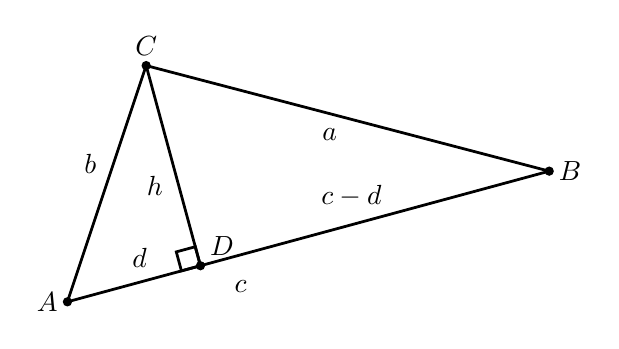
\begin{tikzpicture}[]
\coordinate[label=left:$A$] (A) at (-3,0);
\coordinate[label=right:$B$] (B) at (3.1184,1.6593364341085264);
\coordinate[label=above:$C$] (C) at (-2,3);
\coordinate[label=above right:$D$] (D) at (-1.310642335049465,0.4581610753943723);
\draw [line width=1pt] (A) to[edge label=$b$] (C);
\draw [line width=1pt] (B) to[edge label=$a$] (C);
\draw [line width=1pt] (B) -- (A);
\draw [line width=1pt] (D) to[edge label=$h$] (C);
\draw (-2.3,0.8) node[anchor=north west] {$d$};
\draw (-1,0.4) node[anchor=north west] {$c$};
\draw (0.1,1.6) node[anchor=north west] {$c-d$};
\tkzMarkRightAngle[line width=1pt](A,D,C)
\foreach \p in {A,B,C,D}
	\fill[fill=black,draw=black,thick] (\p) circle (1.25pt);
\end{tikzpicture}
\end{figure*}
\begin{proof}
如上图,由勾股定理:
\begin{align*}
b^2&=h^2+d^2 \\
a^2&=h^2+(c-d)^2
\end{align*}

上面两个式子相减:
\begin{align*}
a^2-b^2&=c^2-2cd \\
d&=\frac{b^2+c^2-a^2}{2c}
\end{align*}

代入第一个式子:
\begin{align*}
h^2&=b^2-d^2=(b+d)(b-d) \\
&=(b+\frac{b^2+c^2-a^2}{2c})(b-\frac{b^2+c^2-a^2}{2c}) \\
&=\frac{(2bc+b^2+c^2-a^2 )(2bc-b^2-c^2+a^2 )}{4c^2} \\
&=\frac{((b+c)^2-a^2 )(a^2-(b-c)^2 )}{4c^2} \\
&=\frac{(b+c+a)(b+c-a)(a+b-c)(c+a-b)}{4c^2} \\
&=\frac{2s\cdot 2(s-a)\cdot 2(s-c)\cdot 2(s-b)}{4c^2} \\
&=\frac{4s(s-a)(s-b)(s-c)}{c^2} 
\end{align*}

求面积:
\begin{equation*}
Area=\frac{1}{2} hc=\sqrt{\frac{1}{4} h^2 c^2 }=\sqrt{s(s-a)(s-b)(s-c)}
\end{equation*}

\end{proof}


\newpage
%------------------------------------------------------------------------------%

\section{欧拉乘积公式}
任意复数 $ s $, 若 $ Re(s) > 1 $, 则 
\[ \sum_n{n^{-s}} = \prod_p{(1-p^{-s})^{-1}}, \]
其中 $ n $ 为正整数, $ p $ 是质数. 等式左边称为黎曼 $ \zeta $ 函数, 右边称为欧拉乘积 $ \epsilon $.

\begin{proof}

\begin{align*}
\zeta(s) &= 1 + \frac{1}{2^s} + \frac{1}{3^s} + \cdots \\
\frac{1}{2^s}\zeta(s) &= \frac{1}{2^s} + \frac{1}{4^s} + \frac{1}{6^s} + \cdots \\
(1-\frac{1}{2^s})\zeta(s) &= 1 + \frac{1}{3^s} + \frac{1}{5^s} + \frac{1}{7^s} + \cdots \\
\frac{1}{3^s}(1-\frac{1}{2^s})\zeta(s) &= \frac{1}{3^s} + \frac{1}{9^s} + \frac{1}{15^s} + \cdots \\
(1-\frac{1}{3^s})(1-\frac{1}{2^s})\zeta(s) &= 1 + \frac{1}{5^s} + \frac{1}{7^s} + \frac{1}{11^s} + \cdots \\
 \vdots & \\
\prod_p{(1-\frac{1}{p^s})}\zeta(s) &= 1.
\end{align*}

将左边的除过去就可以得到:
\[ 
\zeta(s) = \prod_p{(1-p^{-s})^{-1}}.
\]
\end{proof}

另一种证明方法:

考虑欧拉乘积的每一项:
\[ \frac{1}{1-p^{-s}} = 1 + \frac{1}{p^s} + \frac{1}{p^{2s}} + \frac{1}{p^{3s}} + \cdots. \]

将每个质数带入这个式子:
\begin{align*}
\frac{1}{1-2^{-s}} &= 1 + \frac{1}{2^s} + \frac{1}{2^{2s}} + \frac{1}{2^{3s}} + \cdots, \\ 
\frac{1}{1-3^{-s}} &= 1 + \frac{1}{3^s} + \frac{1}{3^{2s}} + \frac{1}{3^{3s}} + \cdots, \\ 
\frac{1}{1-5^{-s}} &= 1 + \frac{1}{5^s} + \frac{1}{5^{2s}} + \frac{1}{5^{3s}} + \cdots, \\ 
\cdots & 
\end{align*}
将它们的乘积展开, 每一项乘积对应了一个正整数的倒数的 $ s $ 次方, 并且是一一对应. 从而说明欧拉乘积公式是成立的.

\newpage
%------------------------------------------------------------------------------%
\section{巴塞尔问题}
全体正整数倒数的平方和为 
\[ \zeta(2)= \frac{1}{1^2} +  \frac{1}{2^2} +  \frac{1}{3^2} +  \cdots = \frac{\pi^2}{6} . \]

\noindent\textbf{欧拉的解法}:

考虑下述函数 $ f(x) $ 的泰勒展开: 
\[ f(x) = \frac{\sin x}{x} = 1 - \frac{x^2}{3!} + \frac{x^4}{5!} + \cdots ,\] 
另一方面, $ f(x) = 0 $ 的根为 $ x = \pm k\cdot \pi $, 所以 $ f(x) $ 又可以表示为:
\[ f(x) = A(1-\frac{x}{\pi}) (1+\frac{x}{\pi}) (1-\frac{x}{2\pi}) (1+\frac{x}{2\pi}) \cdots ,\] 
这里 $ A $ 是待定系数, 通过代入 $ x = 0 $ 可得 $ A = 1 $, 所以
\[ f(x) = (1-\frac{x^2}{\pi^2}) (1-\frac{x^2}{4\pi^2}) (1-\frac{x^2}{9\pi^2}) \cdots ,\] 
比较这两种表达方式的二次项系数, 可得
\[ -\frac{1}{3!} = -(\frac{1}{\pi^2} + \frac{1}{4\pi^2} + \frac{1}{9\pi^2} + \cdots) ,\]
整理之后可得
\[ \frac{\pi^2}{6} = 1 + \frac{1}{4} + \frac{1}{9} + \frac{1}{16} + \cdots \]

\noindent\textbf{常规解法}:

注意到当 $ 0 < \theta < \pi/2 $ 时, 有 $ \sin\theta < \theta < \tan\theta $, 或 $ \cot^2\theta < \dfrac{1}{\theta^2} < \csc^2\theta $. 思路是将所求的正整数倒数的平方和夹在两个求和式之间, 并且上下界都趋于 $ \pi^2/6 $.

令 $ 0 < x < \pi/2 $, $ n $ 是正整数, 引入复数运算: 
\begin{align*} 
\frac{\cos(nx)+i\sin(nx)}{(\sin x)^n} &= \frac{(\cos x+i\sin x)^n}{(\sin x)^n} \\
	 &= \left( \frac{\cos x+i\sin x}{\sin x} \right)^n \\
	&= (\cot x + i)^n
\end{align*}

二项式展开:
\begin{align*}
(\cot x + i)^n &= C_n^0\cot^n x + C_n^1(\cot^{n-1}x)i + \cdots + C_n^{n-1}(\cot x)i^{n-1} + C_n^n i^n\\
				&= \left[ C_n^0\cot^n x - C_n^2\cot^{n-2} x \pm\cdots \right] + i\left[ C_n^1\cot^{n-1} x - C_n^3\cot^{n-3} x \pm\cdots \right]
\end{align*}

这两个复数的实部和虚部应该对应相等, 于是:
\[ \frac{\sin(nx)}{(\sin x)^n} = C_n^1\cot^{n-1} x - C_n^3\cot^{n-3} x \pm\cdots \]

设 $ n = 2m+1 $, 并考虑 $ x_r = \dfrac{r\pi}{2m+1} $, 其中 $ r = 1,2,\cdots,m $, 那么 $ nx_r $ 是 $ \pi $ 的倍数, 意味着 $ x_r $ 是上面式子的零点, 代入上面的式子得:
\[ 0 = C_{2m+1}^1\cot^{2m}x_r - C_{2m+1}^3\cot^{2m-2}x_r \pm\cdots + (-1)^m C_{2m+1}^{2m+1} \]
当 $ r $ 取不同的值时, $ x_r $ 是 $ (0, \pi/2) $ 区间上不同的数, 容易看出 $ \cot^2 x_r $ 也是互不相同的. 令 $ t_r = \cot^2 x_r $, 则 $ t_r $ 是下面 $ m $ 次多项式的根:
\begin{align*} 
p(t) &= C_{2m+1}^1t^m - C_{2m+1}^3t^{m-1} \pm\cdots + (-1)^m C_{2m+1}^{2m+1} \\
	&= A(t-t_1)(t-t_2)\cdots(t-t_m)\\
	&= At^m - A(t_1+t_2+\cdots+t_m)t^{m-1} + \cdots
\end{align*}
比较 $ t^m $ 和 $ t^{m-1} $ 两项的系数可得: $ C_{2m+1}^1(t_1+t_2+\cdots+t_m)=C_{2m+1}^3 $, 所以
\[ \cot^2x_1+\cot^2x_2+\cdots+\cot^2x_m=t_1+t_2+\cdots+t_m=\frac{C_{2m+1}^3}{C_{2m+1}^1}=\frac{2m(2m-1)}{6}\]

另一方面, 根据三角恒等式 $ \csc^2 x = \cot^2 x + 1 $, 得:
\[ \csc^2x_1+\csc^2x_2+\cdots+\csc^2x_m=\frac{2m(2m-1)}{6}+m = \frac{2m(2m+2)}{6} \]

根据前面的不等式 $ \cot^2x<\dfrac{1}{x^2}<\csc^2x $, 因为 $ \dfrac{1}{x_r^2} = \dfrac{(2m+1)^2}{(r\pi)^2} $, 则
\[ \frac{2m(2m-1)}{6} < \frac{(2m+1)^2}{\pi^2}+\frac{(2m+1)^2}{(2\pi)^2}+\cdots+\frac{(2m+1)^2}{(m\pi)^2} < \frac{2m(2m+2)}{6}. \]
这个不等式乘上 $ \dfrac{\pi^2}{(2m+1)^2} $, 得:
\[ \frac{2m(2m-1)\pi^2}{6(2m+1)^2} < \frac{1}{1^2}+\frac{1}{2^2}+\cdots+\frac{1}{m^2} < \frac{2m(2m+2)\pi^2}{6(2m+1)^2}. \]

当 $ m $ 趋于正无穷时, 两端的值都趋于 $ \dfrac{\pi^2}{6} $, 所以 
\[ \zeta(2)=\sum_{k=1}^{\infty}{\frac{1}{k^2}} =\frac{\pi^2}{6}. \]

\noindent\textbf{根据圆导出的解法}:

考虑原点上有一个感光元件, 有一系列一样的单位亮度的灯, 距离原点为 $ d $ 时, 感光元件接收到的光强度是 $ \dfrac{1}{d^2} $.

先证一个引理: 如下图所示, 直角三角形 $ ABC $, 感光元件在直角 $ C $ 上, 直角边长为 $ a $ 和 $ b $, 斜边上的高长 $ h $. 

\begin{wrapfigure}{o}{5.2cm}
\centering
\definecolor{rvwvcq}{rgb}{0.08235294117647059,0.396078431372549,0.7529411764705882}
\definecolor{wrwrwr}{rgb}{0.3803921568627451,0.3803921568627451,0.3803921568627451}
\begin{tikzpicture}[]
\coordinate[label=left:$C$] (C) at (0,0);
\coordinate[label=above:$B$] (B) at (0,3);
\coordinate[label=right:$A$] (A) at (4,0);
\coordinate[label=above right:$D$] (D) at (1.44,1.92);
\tkzMarkRightAngle[line width=1pt](A,C,B);
\tkzMarkRightAngle[line width=1pt](C,D,A);
\draw [line width=1pt] (C) to [edge label=$a$] (B);
\draw [line width=1pt] (A) to [edge label=$b$] (C);
\draw [line width=1pt] (A)-- (B);
\draw [line width=1pt,dash pattern=on 3pt off 3pt] (C) to [edge label=$h$] (D);
\foreach \p in {A,B,C,D}
	\fill[fill=rvwvcq,thick] (\p) circle (1.25pt);
\end{tikzpicture}
\end{wrapfigure}
\indent 根据勾股定理和面积关系, 可以推出:
\begin{align*}
ab &= ch \\
a^2b^2 &= c^2h^2\\
\frac{1}{h^2} &= \frac{c^2}{a^2b^2}=\frac{a^2+b^2}{a^2b^2}\\
\frac{1}{h^2} &= \frac{1}{a^2} + \frac{1}{b^2}
\end{align*}
这意味着当斜边上的垂足上有一个单位亮度的灯时, 感光元件接收的光强等于两个直角顶点上各有一个单位亮度灯时的光强.

现在假定感光元件位于原点 $ O $ 处, 一个小圆的圆心在 $ y $ 轴上, $ OA $ 为直径, 直径是 $ 2/\pi $, 周长为 2. 点 $ A $ 处有一个灯, 则 $ O $ 点的亮度为 $ \pi^2/4 $. 

在小圆外面画一个稍大一点的圆, 直径是小圆的两倍, 两圆内切于 $ O $ 点, 过点 $ A $ 作小圆的切线, 与大圆交于 $ B, C $ 两点. 点 $ OBC $ 构成直角三角形, $ BC $ 是斜边, $ A $ 是斜边上的垂足, 对 $ O $ 点而言, 在 $ B, C $ 两点上各放一个灯, 和在 $ A $ 点放一个灯的亮度是一样的. 

继续在大圆外面画一个更大的圆, 直径是前一个圆的两倍, 为 $ 8/\pi $, 同样与上一个圆相切于 $ O $ 点. 过新的大圆圆心分别作过 $ B $ 和 $ C $ 的直径, 两直径的端点分别是 $ D, E, F, G $, 容易证明这 4 个点平分了圆周. 考虑过 $ C $ 点的直径 $ FD $, $ OFD $ 三点构成直角三角形, $ \angle FOD $ 是直角. 另一方面, $ \angle FCO $ 是第二个圆的直径所对的圆周角, 从而 $ OC $ 是 $ FD $ 上的高. 于是对于 $ O $ 来说, $ C $ 点有一个灯, 等价于 $ F $ 和 $ D $ 上各有一个灯. 同理, $ B $ 点有一盏灯等价于 $ E $ 和 $ G $ 各有一盏灯, 所以 $ DEFG $ 的亮度之和等于 $ A $ 的亮度.

\begin{figure*}[htbp]
\centering
\definecolor{wrwrwr}{rgb}{0.3803921568627451,0.3803921568627451,0.3803921568627451}
\definecolor{rvwvcq}{rgb}{0.08235294117647059,0.396078431372549,0.7529411764705882}
\subfigure{
\begin{minipage}[b]{0.48\linewidth}
\centering
\begin{tikzpicture}[scale=2]
\clip(-1.25,-0.3) rectangle (1.25,2.15);
\coordinate[label=below left:$O$] (O) at (0,0);
\coordinate (C1) at (0,0.5);
\coordinate[label=above left:$A$] (A) at (0,1);
\coordinate[label=left:$B$] (B) at (-1,1);
\coordinate[label=right:$C$] (C) at (1,1);
\draw [line width=1pt] (A) circle (1cm);
\draw [line width=1pt] (C1) circle (0.5cm);
\draw [line width=1pt] (-2.2,0)--(3.1,0);
\draw [line width=1pt] (0,-0.7) -- (0,3.18);
\draw [line width=1pt,dash pattern=on 3pt off 3pt] (B)-- (C);
\foreach \p in {A,B,C,C1,O}
	\fill[fill=rvwvcq,thick] (\p) circle (0.75pt);
\end{tikzpicture} 
\begin{tikzpicture}[scale=2]
\clip(-1.25,-0.3) rectangle (1.25,2.15);
\coordinate[label=below left:$O$] (O) at (0,0);
\coordinate (C3) at (0,1);
\coordinate (C2) at (0,0.5);
\foreach \idx/\lab in {1/P1,-1/P2,3/P3,-3/P4,5/P5,-5/P6,7/P7,-7/P8} {
	\coordinate (\lab) at ({0 + 1*cos(270+\idx*22.5)},{1 + 1*sin(270+\idx*22.5)});
	\fill[fill=wrwrwr,thick] (\lab) circle (0.75pt);
}
\foreach \idx/\lab in {1/D,-1/G,3/E,-3/F} {
	\coordinate (\lab) at ({0 + 0.5*cos(270+\idx*45)},{0.5 + 0.5*sin(270+\idx*45)});
	\fill[fill=wrwrwr,thick] (\lab) circle (0.75pt);
}
\draw [line width=1pt] (C3) circle (1cm);
\draw [line width=1pt] (C2) circle (0.5cm);
\draw [line width=1pt] (-2.2,0)--(3.1,0);
\draw [line width=1pt] (0,-0.7) -- (0,3.18);
\draw (0.2,0.46) node[anchor=north west] {$D$};
\draw (0.05,0.9) node[anchor=north west] {$E$};
\draw (-0.35,0.9) node[anchor=north west] {$F$};
\draw (-0.45,0.4) node[anchor=north west] {$G$};
\draw [line width=1pt,dash pattern=on 3pt off 3pt] (P3)-- (P6);
\draw [line width=1pt] (P6) -- (O)-- (P3);
\draw [line width=1pt] (O) -- (E);
\draw [fill=rvwvcq] (0,1) circle (0.75pt);
\draw [fill=wrwrwr] (0,0) circle (0.75pt);
\end{tikzpicture}
\end{minipage}}
\subfigure{
\begin{minipage}[b]{0.48\linewidth}
\centering
\begin{tikzpicture}[scale=2]
\clip(-1.25,-0.3) rectangle (1.25,2.15);
\def\xx{0.7071067811865475}
\coordinate[label=below left:$O$] (O) at (0,0);
\coordinate[label=right:$B$] (B) at (-0.5,0.5);
\coordinate[label=left:$C$] (C) at (0.5,0.5);
\coordinate[label=135:$A$] (A) at (0,0.5);
\coordinate[label=right:$D$] (D) at (\xx,1-\xx);
\coordinate[label=right:$E$] (E) at (\xx,1+\xx);
\coordinate[label=left:$F$] (F) at (-\xx,1+\xx);
\coordinate[label=left:$G$] (G) at (-\xx,1-\xx);
\coordinate (C2) at (0,1);
\draw [line width=1pt] (C2) circle (1cm);
\draw [line width=1pt] (A) circle (0.5cm);
\draw [line width=1pt] (-2.2,0)--(3.1,0);
\draw [line width=1pt] (0,-0.7) -- (0,3.18);
\draw [line width=1pt,dash pattern=on 3pt off 3pt] (E)-- (G);
\draw [line width=1pt] (F)-- (D);
\draw [line width=1pt] (F)-- (O);
\draw [line width=1pt] (O)-- (D);
\draw [line width=1pt] (O)-- (C);
\foreach \p in {A,B,C,C2,O,E,F,G,D}
	\fill[fill=rvwvcq,thick] (\p) circle (0.75pt);
\end{tikzpicture} 
\begin{tikzpicture}[line cap=round,line join=round,>=triangle 45,x=1cm,y=1cm,scale=2]
\clip(-1.25,-0.3) rectangle (1.25,2.15);
\coordinate[label=below left:$O$] (O) at (0,0);
\coordinate (C4) at (0,16);
\foreach \idx/\lab in {1/P1,-1/P2,3/P3,-3/P4,5/P5,-5/P6,7/P7,-7/P8} {
	\coordinate (\lab) at ({0 + 16*cos(270+\idx*0.5)},{16 + 16*sin(270+\idx*0.5)});
  	\draw [line width=1pt,dash pattern=on 3pt off 3pt] (C4) -- (\lab);
	\fill[fill=wrwrwr,thick] (\lab) circle (0.75pt);
}
\draw [line width=1pt] (-3.8,0) -- (3.4,0);
\draw [line width=1pt] (0,-0.58) -- (0,3.3);
\draw [line width=1pt] (C4) circle (16cm);
\end{tikzpicture}
\end{minipage}}
\end{figure*}
继续在外面画一个更大的圆, 直径是上一个圆的两倍, 过 $ DEFG $ 作大圆的直径, 得到大圆的 8 个等分点, 类似的, 如果这 8 个点上各放一个灯, 它们的亮度之和与 $ A $ 点的亮度是一样的. 另外注意到这一系列圆上, 等分点之间的弧长都是 2.

这个过程一直进行下去, 随着圆越来越大, 曲率越来越小, 得到的等分点在极限情况下都会落在 $ x $ 轴上, 对应的坐标分别是 $ \pm1, \pm3, \cdots $. 这些灯的亮度之和依然是 $ \pi^2/4 $. 即:
\[ \frac{1}{1^2} + \frac{1}{3^2} + \frac{1}{5^2} + \cdots = \frac{\pi^2}{8}. \]
经过简单的代换:
\begin{align*}
\zeta(2) - \frac{1}{4}\zeta(2) &= \left( \frac{1}{1^2} + \frac{1}{2^2} + \frac{1}{3^2} + \cdots \right) - \left( \frac{1}{2^2} + \frac{1}{4^2} + \frac{1}{6^2} + \cdots \right)\\
\frac{3}{4}\zeta(2) &= \frac{1}{1^2} + \frac{1}{3^2} + \frac{1}{5^2} + \cdots = \frac{\pi^2}{8} \\
\zeta(2) &= \frac{\pi^2}{6}
\end{align*}


\newpage
%------------------------------------------------------------------------------%
\section{Leibniz级数与\texorpdfstring{$\pi$}{pi}}

证明: $$ 1 - \frac{1}{3} + \frac{1}{5} - \frac{1}{7} + \cdots = \frac{\pi}{4} $$.

\subsection{中国剩余定理}
假设整数 $ m_1, m_2, \cdots, m_n $ 两两互质, 则对任意的整数 $ a_1, a_2, \cdots, a_n $, 下面的方程组都有解: 
\begin{equation*}
\ \begin{cases}
x\equiv a_{1} & \pmod{m_1}\\
x\equiv a_{2} & \pmod{m_2}\\
\cdots  & \\
x\equiv a_{n} & \pmod{m_n}
\end{cases}
\end{equation*}
并且通解可以用如下方式构造得到: 

设 $ M = m_1\times m_2\times\cdots\times m_n = \prod_{i=1}^{n}{m_i} $, 并设 $ M_i = M / m_i $ 是除了 $ m_i $ 以外的 $ n - 1 $ 个数的乘积, 设 $ t_i = M_i^{-1} $ 是 $ M_i $ 模 $ m_i $ 的逆元: $ M_it_i \equiv 1 \pmod{m_i} $, 则上述方程组的通解为: $ x = x_0 + kM, k\in \mathbb{Z} $, 其中 $$ x_0 = a_1t_1M_1 + a_2t_2M_2\cdots + a_nt_nM_n $$ 是一个特解.

因为当 $ i \neq j $ 时, $ m_i $ 与 $ m_j $ 互质, 则 $ m_i $ 和 $ M_i $ 也互质. 所以 $ M_i $ 模 $ m_i $ 的逆元是存在的, $ a_it_iM_i \equiv a_i \pmod{m_i} $. 另一方面, 当 $ i \neq j $ 时, $ m_i $ 是 $ M_j $ 的因数, 所以 $ a_jt_jM_j \equiv 0 \pmod{m_i}) $. 于是 $ x_0 $是满足方程组的一个解. 

如果有两个解 $ x_1 $ 和 $ x_2 $ 都满足上面的方程组, 对于任意的 $ i\in\{1, 2, \cdots, n\} $, 都有 $ x_1 - x_2 \equiv 0 \pmod{m_i} $, 说明 $ m_i $ 整除 $ x_1 - x_2 $, 而 $ m_1, m_2, \cdots, m_n $ 两两互质, 说明 $ M $ 也整除 $ x_1 - x_2 $, 即任意两个解之差都是 $ M $ 的倍数. 这就证明了上述通解的形式包含了所有的解.

\subsection{欧拉函数}
对正整数 $ x $, 定义欧拉函数 $ \phi(x) $ 为小于或等于 $ x $ 的正整数中, 与 $ x $ 互质的数的数目. 
有以下性质:

\noindent (1) 对任意素数 $ p $, $ \phi(p) = p - 1 $, 这是显然的.

\noindent (2) 对任意素数 $ p $, $ \phi(p^k) = p^k - p^{k-1} = p^k(1-1/p) $. 

这是因为不超过 $ p^k $ 的数中, 与 $ p^k $ 具有相同的因数的数集合为 $ \{ p, 2\times p, \cdots, p^{k-1}\times p \} $, 共 $ p^{k-1} $ 个. 

\noindent (3) 对于任意的素数 $ p, q $, 若 $ p \neq q $, 则 $ \phi(p^mq^n) = \phi(p^m)\phi(q^n) $. 

考虑定义, 不超过 $ p^mq^n $ 的数中, 与 $ p^mq^n $ 不互素的数有 $ p $ 的倍数: $ \{p,2p,\cdots,p^mq^n\} $ 和 $ q $ 的倍数 $ \{q,2q,\cdots,p^mq^n\} $. 两个集合中重复的元素是 $ \{pq, 2pq, \cdots, p^mq^n \} $, 则 $ \phi(p^mq^n) = p^mq^n - p^{m-1}q^{n} - p^{m}q^{n-1} + p^{m-1}q^{n-1} = \phi(p^m)\phi(q^n) $.

\noindent (4) 由上一条容易推断: 对于互质的两个数 $ a, b $, 有 $ \phi(ab) = \phi(a)\phi(b) $.

\noindent (5) 设 $ p_1, p_2, \cdots, p_n $ 为 $ x $ 的所有质因数, 则: $$ \phi(x) = x\prod_{i=1}^{n}{(1-\frac{1}{p_i})} $$.

	对 $ x $ 分解质因数: $ x = p_1^{k_1}p_2^{k_2}\cdots p_n^{k_n} $, 根据 (2) 和 (3), $ \displaystyle \phi(x) = \prod_{i=1}^n\left[p_i^{k_i}(1-\frac{1}{p_i})\right] $, 即得.

\subsection{欧拉定理和费马小定理}

\noindent 欧拉定理: 若 $ a $ 和 $ n $ 互质, 则 $ a^{\phi(n)} \equiv 1 \pmod{n} $. 

\noindent 证明: 设小于 $ n $ 且和 $ n $ 互质的数的集合为 $ \{ X_1, X_2, \cdots, X_m \} $, 其中 $ m = \phi(n) $.

考虑集合 $ \{ aX_1, \cdots, aX_m\} $, 如果 $ aX_i \equiv aX_j \pmod{n} $, 则 $ a(X_i-X_j) \equiv 0 \pmod{n} $, 而 $ n $ 与 $ a $ 互质, 所以 $ X_i - X_j $ 整除 $ n $, 再由 $ X_i, X_j \in [1,n] $, 于是只能是 $ X_i = X_j $. 反过来看, 若 $ X_i \neq X_j $, 则 $ aX_i \neq aX_j $. 所以集合 $ \{aX_i\} $ 也有 $ m $ 个不同元素, 且都与 $ n $ 互质 ( 这是因为 $ a $ 和 $ X_i $ 都与 $ n $ 互质).
 
这意味着集合 $\{aX_i\}$ 和集合 $\{X_i\}$ 在模 $ n $ 下是相同的. 将它们的所有元素乘起来:
$$ X_1\cdot X_2\cdots X_m \equiv aX_1\cdot aX_2\cdots aX_m \pmod{n} $$ 
亦即 $ (a^m - 1)\prod{X_i} \equiv 0 \pmod{n} $.

因为 $ X_i $ 和 $ n $ 互质, 所以 $ a^m - 1 \equiv 0 \pmod{n} $, 或 $ a^{\phi(n)} \equiv 1 \pmod{n} $.

~

\noindent 费马小定理: 若 $ a $ 和素数 $ p $ 互质, 则 $ a^{p-1} \equiv 1 \pmod{p} $. 这是欧拉定理的特例.

\subsection{有限差分}

命题: 序列 $ 1^k, 2^k, 3^k, \cdots, n^k, \cdots $ 的 $ k $ 阶差分序列全都等于 $ k! $. 其中 $ i $ 阶差分序列的定义为 $ D^{(i)}_n = D^{(i-1)}_{n+1} - D^{(i-1)}_n, \ n\in\mathbb{N} $; $ 0 $ 阶差分就是原序列: $ D^{(0)}_n = x_n $.

用归纳法可证明. 首先当 $ k = 1 $ 时, 差分序列为 $ 1, 1, \cdots $, 结论成立.

假设命题对于任意 $ k = 1, 2, \cdots, m - 1 $ 都成立, 考虑 $ k = m $, 为了算 $m$ 阶差分, 先算一阶的. 它的一阶差分序列通项为 
$$ D^{(1)}_n = (n+1)^{m} - n^m = 1 + C_m^1n + C_m^2n^2+\cdots+C_m^{m-1}n^{m-1} .$$ 

先考虑前 $ m - 2 $ 项, 接下来要做 $ m - 1 $ 次差分, 由归纳假设, $ n $ 的一次方项经过一次差分变成 $ 1!C_m^1 $, 平方项经过2次差分变成 $ 2!C_m^2 $, 等等, 它们都是常数, 到 $ m - 1 $ 次差分的时候都变成了 $ 0 $; 而最后一项经过 $ m - 1 $ 次差分变成了 $ (m-1)!C_m^{m-1} = m! $. 

说明当 $ k = m $ 的时候也成立. 所以命题得证.

\subsection{\texorpdfstring{$4k+1$}{4k+1}型素数的平方和分解}

\noindent 定理: 如果素数 $ p $ 模 $ 4 $ 余数是 $ 1 $, 则存在唯一一对整数 $a,b$, 使得 $ p = a^2 + b^2 $.

先证明存在性, 这里介绍欧拉的方法, 分为 5 个步骤.

\noindent (1) 若 $ x,y $ 都是两个整数的平方和, 则它们的乘积也是两个整数的平方和.

证明: 设 $ x = a^2+b^2, y = p^2+q^2 $, 则 \[ xy = (a^2+b^2)(p^2+q^2)=(ap+bq)^2+(aq-bp)^2 .\]

~

\noindent (2) 若 $ x,y $ 都是两个整数的平方和, $ y $ 是素数, 且 $ y $ 整除 $ x $, 则 $ x/y $ 也是两个整数的平方和.

证明: 设 $ x = a^2+b^2, y = p^2+q^2 $, 考虑下面的关系:
\begin{align*} 
z = (pb-aq)(pb+aq) & = p^2b^2-a^2q^2 \\
	& = p^2(a^2+b^2)-a^2(p^2+q^2)\\
	& =p^2x-a^2y.
\end{align*}

因为 $ y $ 整除 $ x $, 则 $ y $ 也整除 $ z $. 又因为 $ y $ 是素数, 所以 $ y $ 一定整除 $ pb-aq $ 或 $ pb + aq $. 先假设 $ y $ 整除 $ pb-aq $, 观察到
\[ xy = (a^2+b^2)(p^2+q^2)=(ap+bq)^2+(aq-bp)^2 ,\]
两边除以 $ y^2 $:
\[ \frac{x}{y} = \left(\frac{ap+bq}{y}\right)^2+\left(\frac{bp-aq}{y}\right)^2 .\]

$ y $ 整除 $ pb-aq $ 和 $ x $, 等式两边都是整数, 所以 $ y $ 也必须整除 $ ap+bq $. 这里 $ x/y $ 就已经是两个整数的平方和了.

如果$ y $ 整除 $ pb+aq $, 类似的有
\[ xy = (a^2+b^2)(p^2+q^2)=(aq+bp)^2+(ap-bq)^2 ,\]
也能成立.

~

\noindent (3) 若 $ x $ 是两个整数的平方和, $ y $ 整除 $ x $, 且 $ y $ 不能表示成两个整数的平方和, 则 $ x/y $ 也存在一个因子无法写成两整数平方和.

证明: 对 $ x/y $ 做素因数分解: $ x/y=p_1p_2\cdots p_n $. 如果所有的 $p_i$ 都能写成两整数的平方和, 反复应用上面第(2)条, 可以推出 $ x/p_1 $ 能写成两个整数平方和, $ x/(p_1p_2) $ 也能, 等等, 一直到 $ x/(p_1p_2\cdots p_n)=y $ 也是两个整数平方和.这与条件矛盾.

~

\noindent (4) 若 $ a,b $ 互素, 则 $ a^2+b^2 $的所有因数都能表示成两个整数平方之和.

证明: 如果 $ a^2 + b^2 $ 是素数, 命题已经得证. 假设 $ q $ 是 $ a^2+b^2 $ 的任一因数. $q=2$时也显然成立. 下面考虑 $ q > 2 $ 的情况.

选取非负整数 $ m $ 和 $ n $, 使得 $mq$ 和 $nq$ 分别是距离 $a$和$b$的最近的 $q$的倍数. 有没有可能 $q$是偶数且 $|mq-a| = q/2 $ 呢? 如果是这样, 则 $q/2$ 一定是 $ a $ 的因数, 而 $ q $ 是 $a^2+b^2$ 的因数, 所以$ q/2 $ 也是 $a^2+b^2$ 的因数, 这就说明 $q/2$ 也是 $b$ 的因数, 这与 $ a,b $ 互素矛盾.

令 $ c=mq-a, d=nq-b$. 则 $ |c| < q/2, |d| < q/2 $. 
\[ a^2 + b^2 = (mq-c)^2+(nq-d)^2 = Aq+(c^2+d^2) ,\]
这里 $ A $ 是一个合适的整数.

因为 $q$ 是 $a^2+b^2$的因数, 上式表明 $q$ 也是 $ ( c^2 + d^2 ) $ 的因数. 于是令 $ c^2 + d^2 = qr $, 并设 $ c,d $ 的最大公约数为 $ g $, 则可知 $ g $ 与 $ q $ 互质. (否则由 $ a=c+mq $ 和 $ b=d+nq $, $gcd(g,q)$ 也能整除 $a$ 和 $b$, 与 $a,b$ 互素矛盾.)

再由 $ g^2 $ 整除 $ qr $, 得 $ g^2 $ 是 $ r $ 的因数. 设 $ r = sg^2, e=c/g, f=d/g $. 则
\[ qs = \frac{qr}{g^2}=e^2+f^2\leq c^2+d^2 < (\frac{q}{2})^2 + (\frac{q}{2})^2 = \frac{q^2}{2} \] 
不等式两边约去 $ q $ 得到 $ s < q/2 $. 

因为 $ qs $ 是两整数平方和, 如果 $ q $ 不能写成两整数平方和, 则根据上面第(3)条, $ s $ 存在一个因数 $ q_1 $ 不能写成两整数平方和, $ q_1 \leq s < q/2 < q $. 现在有 $ e,f $ 互素, $ q_1 $ 是 $ e^2+f^2 $ 的因数, 重复上面的构造过程 ( $a,b,q$ 分别换成 $e,f,q_1$), 将得到 $q_2 < q_1$, 反复构造将得到一个严格递减的无穷正整数序列, 这是不可能的. 所以 $ q $ 可以写成两整数平方和.

~

\noindent (5) 任意 $ 4n + 1 $ 形式的素数都能写成两个整数的平方和.

证明: 设 $ p = 4n + 1 $, 由费马小定理, 对任意的 $ a $, 都有 $ a^{4n} \equiv 1 \pmod{p} $. 令 $ a $ 取 $ 1, 2, \cdots, 4n $, 则序列 $ S = \left[2^{4n}-1^{4n}, \cdots, (4n)^{4n}-(4n-1)^{4n} \right] $ 中的每一项都可以被 $ p $ 整除. 分析它们的通项: \[ a^{4n}-b^{4n}=(a^{2n}+b^{2n})(a^{2n}-b^{2n}),\] 
其中 $ a=b+1 $, 于是 $a,b$ 互素.

因为 $p$ 是素数, 所以 $p$ 整除 $ a^{2n}+b^{2n} $ 或 $ a^{2n}-b^{2n} $. 如果上述序列 $ S $ 的 $ 4n-1 $ 项中有一项是 $p$ 整除 $ a^{2n}+b^{2n} $, 根据上面的第(4)条, 可知 $p$ 可以表示成两整数的平方和. 

反之, 如果全部 $ 4n-1 $ 种情况下都是 $p$ 整除 $ (b+1)^{2n}-b^{2n} $, 我们从有限差分的性质推出这是不可能的.
考虑序列 $ 1^{2n}, 2^{2n}, \cdots, (4n)^{2n} $, 根据假设, 它的一阶差分都是 $p$ 的倍数, 从而更高阶的差分也都是 $ p $ 的倍数. 特别地, 取 $ 2n $ 阶差分, 它每一项都等于 $ (2n)! $, 因为 $ p $ 是素数, $ 2n < 4n + 1 = p $, 说明 $(2n)!$ 不可能被 $p$ 整除, 矛盾.

~

下面证明$4k+1$型素数的平方和分解的唯一性.

如果存在两种分解方式 $ p = a^2+b^2=c^2+d^2 $, 不妨设 $a,b,c,d $ 都是正整数, 注意到
\begin{align*} 
p^2=(a^2+b^2)(c^2+d^2) & =(ac+bd)^2+(ad-bc)^2 \\ & =(ac-bd)^2+(ad+bc)^2 .\end{align*}
此外由 $ (p-a^2)d^2=(p-c^2)b^2 $, 可得 $ p(d^2-b^2)=(ad-bc)(ad+bc) $.

$ p $是素数, 若 $p$ 整除 $ ad-bc$, 由 $p^2=(ac+bd)^2+(ad-bc)^2$, 知 $ (ad-bc)^2 = p^2-(ac+bd)^2 < p^2 $, 从而 $ ad-bc=0 $. 于是 $ d^2=b^2 $, 说明两种分解方式是相同的.

若 $p$ 整除 $ad+bc$, 由 $p^2=(ac-bd)^2+(ad+bc)^2$ 知 $ (ad+bc)^2 = p^2 $, 从而 $ ac = bd $. 又易知 $a,b$ 互素, 所以 $ a $ 整除 $ d $ 且 $ b $ 整除 $ c $. 不难得到 $ a=d, b=c $.


\subsection{高斯整数和高斯素数}

高斯整数定义为复数集合 $ \mathbb{Z}\left[i\right] = \{ a + bi\ |\ a,b\in\mathbb{Z},\ i^2=-1\} $, 也就是复平面上的整点. 

同整数的素数分解一样, 高斯整数也有素数分解, 但不唯一. 考虑 $ z = x\cdot y $, 同时也有 $ z = (ix)\cdot(-iy) = (-x)\cdot(-y) = (-ix)\cdot(iy) $. 这 4 种分解方式本质上都是一样的.

再考虑共轭复数的分解. 如果 
$$ z = x\cdot y = (a+bi)(c+di) = (ac-bd)+i(ad+bc), $$ 则 $$ \bar{z} = (ac-bd)-i(ad+bc) = (a-bi)(c-di) = \bar{x}\bar{y}. $$ 这说明了共轭复数的分解存在一一对应关系.

观察 $ z\bar{z}= (x\bar{x})(y\bar{y}) $, 左边是一个实整数, 右边每一对共轭因子的乘积也是实整数. 我们对 $ z $ 的模长平方做素数分解, 再将所得的每个素因子分解成一对共轭复数的乘积, 就可以得到 $ z\bar{z} $ 的高斯素数分解. 每对因子 $ x $ 和 $ \bar{x} $ 种有且只有一个能被 $ z $ 整除, 只要试一下就知道该取哪一个作为 $ z $ 的因子.

素的实整数 $ p $ 能否分解成共轭复数的乘积? 等价于求整数 $ a, b $ 满足 $ a^2 + b^2 = p $.

若 $ p = 2 $, 有 $ 2 = 1^2 + 1^2 = (1+i)(1-i) $.

若 $ p = 4k + 3 $, 先考虑 $ a, b \bmod{4} $ 的结果, 可能有 $\{0, 1, 2, 3\} $ 这些情况; 而 $ a^2, b^2 \bmod{4} $ 只有 $ \{0, 1\} $ 两种情况; $ a^2 + b^2 \bmod{4} $ 的取值范围为 $ \{0,1,2\} $. 于是 $ p = 4k + 3 $ 类型的素数无法进一步分解.

若 $ p = 4k + 1$, 存在唯一的分解方式.

\subsection{半径为 \texorpdfstring{$ \sqrt{n} $}{sqrtn} 的圆周上的整点个数}

考虑圆心在原点, 半径为 $ R $ 的圆, 当 $ R $ 足够大时, 圆内的整点数量和圆的面积趋近于相等. 因此如果知道圆内整点数量和半径 $ R $ 的关系, 就能求出 $ \pi $ 的一种逼近方式.

整点到原点的距离平方都是整数, 为了数出圆内整点个数, 可以将它们按同心圆归类. 例如, 半径为 $ 1 $ 的圆上有 $ 4 $ 个整点, 而半径为 $ \sqrt{5} $ 的圆上有 $ 8 $ 个, 半径 $ 5 $ 的圆上有 $ 12 $ 个. 只要数清楚半径为 $ \sqrt{n} $ 上有多少整点. 这等价于求 $ x^2+y^2 = n $ 的整数解个数, 或者说求 $ n $ 在复数域上的分解 $ n = (x+iy)(x-iy) $ 的个数.

先考虑 $ n $ 是素数的情况, 此时仅当 $ n $ 是 $ 4k + 1 $ 的形式才有唯一的平方和分解: $ n = a^2 + b^2 = (a+bi)(a-bi) $, 取其中这对共轭因子的任意一个, 将它乘以 $ \pm 1 $ 和 $ \pm i $, 可以得到 8 个不同的复数, 对应了 $ (\pm a, \pm b), (\pm b, \pm a) $ 共 $8$ 个整点. 特别的, 当 $ n = 2 $ 时, $ a = b = 1 $, 这 $8$ 个点有一半是重复的.

再考虑 $ n $ 是素数的整数次幂的情况: $ n = p^m $. 当 $ p = 4k + 3 $ 时, 只有 $ m $ 是偶数才存在分解 $ n = (p^\frac{m}{2})^2 + 0^2 $, 对应两坐标轴上的 $4$ 个整点. 当 $ p = 4k + 1 = a^2+b^2 $ 时, $ n = (a+bi)^m(a-bi)^m $, 需要在这 $ m $ 对共轭因子中凑出两对共轭的乘积 $ (x\pm iy) $, 所以每一对因子其中一个贡献给 $(x+iy)$, 另一个贡献给 $(x-iy)$. 这些因子一共可以乘出 $m+1$ 个不同的乘积 $ (x\pm iy) $, 分别是 $(a+bi)^l(a-bi)^{m-l} $, $ 0 \le l \le m $. 这些乘积经过 $ \pm 1 $ 和 $ \pm i $ 旋转后有 $ 4(m+1) $ 个整点. 特别的, 当 $ p = 2 $ 时, 仍然存在大量重复的点, 实际上不同的点只有坐标轴上的 $4$ 个.

最后考虑一般的情况, 对 $ n $ 做素数分解, 设素因数 $ p_i $ 对应的指数为 $ m_i $, 则 $ p_i^{m_i} $ 可以生成 $ 0, 1, m+1 $ 种不同的 $(x_i+iy_i)$, 取决于 $ p_i $ 和 $ m_i $ 的取值 ( 注意这里去掉了乘以 $ \pm 1 $ 和 $ \pm i $ 的旋转对称的情况 ). 不同素因数分解出来的 $(x_i+iy_i)$ 可以自由组合, 不会乘出来重复的数, 所以, $ n $ 分解出来的高斯整数是各个不同因数对应的分解个数乘起来.

% \subsection{$\chi$ 函数}

现定义一个正整数上的函数 $ \chi(n) $ : 
\begin{equation*}
\chi(n) = \begin{cases}
0,\ \ if \ n \equiv 0 \pmod{2}\\
1,\ \ if \ n \equiv 1 \pmod{4}\\
-1,\ \ if \ n \equiv 3 \pmod{4}
\end{cases}
\end{equation*}
不难验证 $ \chi(mn) = \chi(m)\chi(n) $ 对任意正整数 $ m, n $ 都成立.

回到圆周上的整点问题, 当 $ n $ 是素数的整数次幂, $ n=p^m=(x+iy)(x-iy) $ 的分解出来的(共轭)复数有 $ F(p,m) = 1 + \chi(p) + \chi(p^2) + \cdots + \chi(p^m) $ 这么多个. ( 同样忽略了旋转对称.) 可以验证, 对于 $ p = 2 $, $ p = 4k+1 $, 和 $ p=4k+3 $ 型的素数都是成立的. 

于是对于 $ n = \prod{p_i^{m_i}} $, 分解出来的高斯整数个数是 $ G(n) = \prod{F(p_i,m_i)} $. 可以把这个乘积展开, 并利用 $ \chi $ 函数的可乘性. 则 $ G(n) = \sum_{d|n}{\chi(d)} $, 也就是对 $ n $ 的所有因数求 $ \chi $ 函数值, 再加起来. 

\subsection{半径 \texorpdfstring{$ R $}{R} 的圆内的整点个数}
令 $ n $ 从 $ 1 $ 取到 $ R^2 $, 对上面的结论分别求 $ G(n) $, 并求和, 就得到半径 $ R $ 的圆内的整点个数. 现在观察不同的 $ \chi $ 函数出现了多少次.
\begin{align*}
G(1) &= \chi(1) \\
G(2) &= \chi(1) + \chi(2) \\
G(3) &= \chi(1) + \chi(3) \\
G(4) &= \chi(1) + \chi(2) + \chi(4) \\
G(5) &= \chi(1) + \chi(5) \\
G(6) &= \chi(1) + \chi(2) + \chi(3) + \chi(6)\\
\cdots
\end{align*}

对每个 $d$, $ \chi(d) $ 都会在 $ G(kd) $ 里都会出现, 也就是每隔 $d$ 行出现一次.
于是 $ R^2 $ 行里出现次数为 $ R^2/d $.
将他们加起来, 并考虑 4 倍的旋转对称:
\[ \pi R^2 \approx 4\sum_{n=1}^{R^2}{G(n)} = 4R^2\left( 1 + \frac{\chi(2)}{2} + \frac{\chi(3)}{3} + \cdots + \frac{\chi(R^2)}{R^2} \right) .\]

把 $ \chi $ 函数的值代进去, 并令 $ R $ 趋于无穷, 约等于就变成等于:
\[ \frac{\pi}{4} = 1 - \frac{1}{3} + \frac{1}{5} -\frac{1}{7} + \cdots \]

\newpage
%------------------------------------------------------------------------------%

\section{Wallis 乘积}

Wallis 乘积公式: \[ \frac{\pi}{2} = \frac{2}{1}\cdot\frac{2}{3}\cdot\frac{4}{3}\cdot\frac{4}{5}\cdot\frac{6}{5}\cdot\frac{6}{7}\cdots \]

先证明一个引理: 单位圆上有 $ N $ 个等分点, 其中相邻两个点之间的圆弧的中点到所有这些等分点的直线距离的乘积恒等于 $ 2 $; 而某个等分点到其余等分点的直线距离的乘积等于 $ N $.

考虑复数域上的方程 $x^N-1=0 $ , 它有 $ N $ 个复数根 $ x_k = e^{k\omega i}$, 其中 $ \omega = \frac{2\pi}{N}, k=0,1,\cdots,N-1 $. 这些根正好是复平面上单位圆的 $ N $ 个等分点. 所以原方程写成根式的形式: \[ x^N - 1 = (x - x_0)(x - x_1)\cdots(x-x_{N-1}) .\] 它对于任意的复数 $ x $ 当然也是成立的. 设 $ f \in (0,1) $, 取一点 $ X_f =  e^{f\omega i} $, 对应 $ x_0 $ 到 $ x_1 $ 之间占比为 $ f $ 的复数点. 对它取 $ N $ 次方自然是得到整个圆周占比为 $ f $ 的复数点 $e^{2\pi fi}$ . 代入上面的公式, 并对两边取模得到:
\[ || X_f^N-1 || = ||(X_f-x_0)||\cdot||(X_f - x_1)||\cdots||(X_f-x_{N-1})|| .\]

观察左边是复数 $e^{2\pi fi}$ 到 $ 1 $ 的距离, 右边是 $ N $ 个距离的乘积. 将 $\displaystyle f = \frac{1}{2} $ 代入, 左边是 $ 2 $, 右边是 $ x_0 $ 到 $ x_1 $ 之间圆弧的中点到其他各个复数根时间的距离之积. 引理第一条得证.

\begin{figure*}[htbp]
\definecolor{ududff}{rgb}{0.30196078431372547,0.30196078431372547,1}
\definecolor{rvwvcq}{rgb}{0.08235294117647059,0.396078431372549,0.7529411764705882}
\definecolor{uuuuuu}{rgb}{0.26666666666666666,0.26666666666666666,0.26666666666666666}
\centering
\begin{minipage}[t]{0.49\linewidth}
\begin{tikzpicture}[scale=0.6]
\coordinate[] (O) at (0,0);
\coordinate[label=below right:$x_0$] (A) at (4,0);
\coordinate[label=above:$x_1$] (B) at (1.2360679774997898,3.804226065180614);
\coordinate[label=left:$x_2$] (C) at (-3.2360679774997894,2.3511410091698925);
\coordinate[label=left:$x_3$] (D) at (-3.23606797749979,-2.351141009169892);
\coordinate[label=below:$x_4$] (E) at (1.2360679774997891,-3.8042260651806146);
\coordinate[label=above right:$x$] (X) at (3.23606797749979,2.3511410091698925);
\clip(-5.5,-5.5) rectangle (6.5,6.0);
\draw[rvwvcq,->,line width=1pt] (-5.0,0) -- (5.5,0) node[right] {$x$};
\draw[rvwvcq,->,line width=1pt] (0,-5.0) -- (0,5.0) node[above] {$y$};
\draw [line width=1.25pt] (O) circle (4cm);
\draw [line width=1.25pt] (A)-- (X);
\draw [line width=1.25pt] (X)-- (B);
\draw [line width=1.25pt] (X)-- (C);
\draw [line width=1.25pt] (X)-- (D);
\draw [line width=1.25pt] (X)-- (E);
\draw (3.8,2.0) node[anchor=north west] {$x-x_0$};
\draw (0.9,4.2) node[anchor=north west,rotate=-36] {$x-x_1$};
\draw (-2.2,2.38) node[anchor=north west] {$x-x_2$};
\draw (-2.1,-1.5) node[anchor=north west,rotate=36] {$x-x_3$};
\draw (0.6,-3.1) node[anchor=north west,rotate=72] {$x-x_4$};
\begin{scriptsize}
\draw [fill=uuuuuu] (O) circle (2pt);
\draw [fill=ududff] (A) circle (2.5pt);
\draw [fill=ududff] (B) circle (2.5pt);
\draw [fill=ududff] (C) circle (2.5pt);
\draw [fill=ududff] (D) circle (2.5pt);
\draw [fill=ududff] (E) circle (2.5pt);
\draw [fill=ududff] (X) circle (2.5pt);
\end{scriptsize}
\end{tikzpicture}
\end{minipage}
\begin{minipage}[t]{0.49\linewidth}
\begin{tikzpicture}[scale=0.6]
\coordinate[] (O) at (0,0);
\coordinate[label=below right:$x_0$] (A) at (4,0);
\coordinate[label=above:$x_1$] (B) at (1.2360679774997898,3.804226065180614);
\coordinate[label=left:$x_2$] (C) at (-3.2360679774997894,2.3511410091698925);
\coordinate[label=left:$x_3$] (D) at (-3.23606797749979,-2.351141009169892);
\coordinate[label=below:$x_4$] (E) at (1.2360679774997891,-3.8042260651806146);
\clip(-5.5,-5.5) rectangle (6.5,6.0);
\draw[rvwvcq,->,line width=1pt] (-5.0,0) -- (5.5,0) node[right] {$x$};
\draw[rvwvcq,->,line width=1pt] (0,-5.0) -- (0,5.0) node[above] {$y$};
\draw [line width=1.25pt] (O) circle (4cm);
\draw [line width=1.25pt] (A) -- (B);
\draw [line width=1.25pt] (A)-- (C);
\draw [line width=1.25pt] (A)-- (D);
\draw [line width=1.25pt] (A)-- (E);
\draw (1.8,3.2) node[anchor=north west,rotate=-54] {$x_0-x_1$};
\draw (-2.2,2.0) node[anchor=north west,rotate=-18] {$x_0-x_2$};
\draw (-2.5,-1.2) node[anchor=north west,rotate=18] {$x_0-x_3$};
\draw (0.8,-3.0) node[anchor=north west,rotate=54] {$x_0-x_4$};
\begin{scriptsize}
\draw [fill=uuuuuu] (O) circle (2pt);
\draw [fill=ududff] (A) circle (2.5pt);
\draw [fill=ududff] (B) circle (2.5pt);
\draw [fill=ududff] (C) circle (2.5pt);
\draw [fill=ududff] (D) circle (2.5pt);
\draw [fill=ududff] (E) circle (2.5pt);
\end{scriptsize}
\end{tikzpicture}
\end{minipage}
\end{figure*}

另一方面, 为了求出 $ x_0 = 1 $ 到其他根的距离之积, 对 $ x^N - 1 $ 做因式分解: 
\[ x^N-1 = (x-1)(1+x+x^2+\cdots+x^{N-1}) ,\]
于是
\[ ||x-x_1||\cdot||x-x_2||\cdots||x-x_{N-1}|| = \frac{||x^N-1||}{||x-1||} = || 1+x+x^2+\cdots+x^{N-1} || .\] 
把 $ x = 1 $ 代入上式, 左边是其中一个根到其他所有根的距离之积, 右边是 $ N $, 引理第二条也得证.

然后, 考虑两个点 $ A = 1, B = e^{\frac{1}{2}\omega i} $, 并记单位圆上 $ A $ 点逆时针方向的等分点为 $ x_1, x_2, \cdots $, 顺时针方向的点为 $ x_{-1}, x_{-2}, \cdots $. 计算下面的比值:
\[ P = \frac{||A-x_1||}{||B-x_1||} \frac{||A-x_{-1}||}{||B-x_{-1}||} \cdot \frac{||A-x_2||}{||B-x_2||} \frac{||A-x_{-2}||}{||B-x_{-2}||} \cdots \]

\begin{figure*}[htbp]
\definecolor{qqwuqq}{rgb}{0,0.39215686274509803,0}
\definecolor{ududff}{rgb}{0.30196078431372547,0.30196078431372547,1}
\definecolor{uuuuuu}{rgb}{0.26666666666666666,0.26666666666666666,0.26666666666666666}
\centering
\begin{tikzpicture}[cap=round,scale=3.0]
\coordinate[] (O) at (0,0);
\coordinate[label=below right:$A$] (A) at (4,0);
\coordinate[label=right:$B$] (B) at (3.9945181390182953,0.20934382497177534);
\coordinate[label=right:$x_1$] (C) at (3.9780875814730927,0.4181138530706139);
\coordinate[label=right:$x_2$] (D) at (3.912590402935222,0.8316467632710373);
\coordinate[label=right:$x_{-1}$] (E) at (3.978087581473093,-0.4181138530706139);
\coordinate[label=right:$x_{-2}$] (F) at (3.9125904029352223,-0.8316467632710373);
\clip(-0.1,-1.0) rectangle (4.1,1.0);
\draw [line width=1.5pt] (O) circle (4cm);
\draw [line width=1.5pt] (O) -- (A);
\draw [dashed,line width=1.5pt] (O) -- (B);
\draw [fill=uuuuuu] (O) circle (0.75pt);
\draw [fill=ududff] (A) circle (0.75pt);
\draw [fill=ududff] (B) circle (0.75pt);
\draw [fill=ududff] (C) circle (0.75pt);
\draw [fill=ududff] (D) circle (0.75pt);
\draw [fill=ududff] (E) circle (0.75pt);
\draw [fill=ududff] (F) circle (0.75pt);
\draw (2.5,-0.1) node[anchor=north west] {$\theta = \frac{1}{2}\omega=\frac{\pi}{N}$};
\draw
    pic["$\theta$",draw,line width=1pt, angle eccentricity=1.5, angle radius=5.5cm] {angle=A--O--B};

\end{tikzpicture}
\end{figure*}

根据上面的引理, 可以得:
\begin{align*}
||A-x_1||\cdot ||A-x_{-1}||\cdot||A-x_2||\cdot||A-x_{-2}||\cdots &= N \\
||B-A||\cdot||B-x_1||\cdot ||B-x_{-1}||\cdot||B-x_2||\cdot||B-x_{-2}||\cdots &= 2
\end{align*}
比较一下, 可以得到 
\[ P =  \frac{N||B-A||}{2}.\]

弦 $ AB $ 的圆心角为 $ \theta=\dfrac{2\pi}{2N} $, 当 $ N $ 很大时, 这个角度很小, 则弦长近似等于弧长, 半径为$ 1 $, 所以 \[ ||B-A|| = \frac{2\pi}{2N}\cdot 1 .\]
代入得到\[ P = \frac{N||B-A||}{2} = \frac{\pi}{2} \]

同样的, 再看 $ A $ 到点 $ x_{\pm k} $ 的弧对应的圆心角都是 $ 2k\theta $, 点 $ B $ 到 $ x_{\pm k} $ 的圆心角分别是 $ (2k\pm 1)\theta $. 当 $ N $ 很大时, 弦长近似等于弧长. 原来 $ P $ 的表达式右边的连乘式为: 
\[ P = \frac{||A-x_1||}{||B-x_1||} \frac{||A-x_{-1}||}{||B-x_{-1}||} \cdot \frac{||A-x_2||}{||B-x_2||} \frac{||A-x_{-2}||}{||B-x_{-2}||} \cdots = \frac{2}{1}\cdot\frac{2}{3}\cdot\frac{4}{3}\cdot\frac{4}{5}\cdot\frac{6}{5}\cdot\frac{6}{7}\cdots ,\]
这也就证明了 Wallis 公式.

~

\noindent 另一种证法: (来自 MAA Monthly)

定义序列 $ s_1= 1 $, 对于 $ n \ge 2 $, \[ s_n = \frac{3}{2}\cdot\frac{5}{4}\cdots\frac{2n-1}{2n-2} .\]
再定义 $ o_n $ 和 $ e_n $: 
\begin{align*}
o_n &= \frac{2^2\cdot 4^2\cdots (2n-2)^2\cdot (2n)}{1\cdot 3^2\cdots (2n-1)^2} = \frac{2n}{s_n^2} ,\\
e_n &= \frac{2^2\cdot 4^2\cdots (2n-2)^2}{1\cdot 3^2\cdots (2n-3)^2\cdot (2n-1)} = \frac{2n-1}{s_n^2} .
\end{align*}
显然有 $ e_n < e_{n+1} $ 和 $ o_n > o_{n+1} $, 以及 $ e_n < o_n $. 于是:
\[ e_1 < e_2 < e_3 < \cdots < o_3 < o_2 < o_1 .\]
所以, 对于 $ 1\le i < n $, 有 \[ \frac{2i}{s_i^2}=o_i\ge o_n \] 和 \[ \frac{2i-1}{s_i^2}=e_i\le e_n ,\]
可以推出 \[ \frac{2i-1}{e_n}\le s_i^2\le \frac{2i}{o_n} .\]

如果定义 $ s_0 = 0 $, 则上面的不等式对于 $ i = 0 $ 也是成立的.  记 $ a_n = s_{n+1} - s_n $, 观察到 $ a_0 = 1 $, 对于 $ n \ge 1 $, 
\[ a_n = s_{n+1}-s_n = s_n\left(\frac{2n+1}{2n} - 1 \right) = \frac{s_n}{2n} = \frac{1}{2}\cdot\frac{3}{4}\cdots\frac{2n-1}{2n} .\]

对于任意 $ i, j $, 因为 \[ a_{i+1} = \frac{2i+1}{2(i+1)}a_i \]
考虑下面的和:
\begin{align*}
\frac{j+1}{i+j+1}a_i a_{j+1} + \frac{i+1}{i+j+1}a_{i+1}a_j &= \frac{a_i a_j}{i+j+1}\cdot\left((j+1)\frac{2j+1}{2(j+1)} + (i+1)\frac{2i+1}{2(i+1)}\right) \\
 &= a_i a_j.
\end{align*}
由这个等式可以得到递推的等式: 
\begin{align*} 
 & a_0a_{n-1}+a_1a_{n-2}+\cdots+a_{n-1}a_0 \\
= &\left(a_0a_n+\frac{1}{n}a_1a_{n-1}\right)+\left(\frac{n-1}{n}a_1a_{n-1}+\frac{2}{n}a_2a_{n-2}\right)+\cdots+\left(\frac{1}{n}a_{n-1}a_1+a_na_0\right) \\
 = & a_0a_n + a_1a_{n-2} + \cdots + a_na_0 . 
\end{align*}
从 $ i = j = 0 $ 出发, 反复应用上面的等式, 可以得到 
\begin{align*}
1 &= a_0^2 = a_0a_1 + a_1a_0 = a_0a_2+a_1^2+a_2a_0 = \cdots \\
  &= a_0a_n + a_1a_{n-1} + \cdots + a_na_0 .
\end{align*}

将 $ xy $ 平面第一象限划分成一些矩形区域, 矩形的边分别是 $ x = s_n $ 和 $ y = s_n $, 令 $ R_{i,j} $ 是左下角为 $ (s_i, s_j) $, 右上角为 $ (s_{i+1}, s_{j+1} ) $ 的矩形. 记矩形 $ R_{i,j} $ 的面积为 $ a_{i,j} $, 根据上一个等式, 所有满足 $ i + j = n $ 的矩形 $ R_{i,j} $ 的面积之和是 $ 1 $. 令 $ P_n $ 是 所有满足 $ i+j < n $ 的矩形构成的多边形区域, 可知 $ P_n $ 的面积是 $ n $. 下图显示了 $ P_4 $ 包含的区域.
\begin{figure*}[htbp]
\definecolor{qqwuqq}{rgb}{0,0.39215686274509803,0}
\definecolor{ududff}{rgb}{0.30196078431372547,0.30196078431372547,1}
\definecolor{uuuuuu}{rgb}{0.26666666666666666,0.26666666666666666,0.26666666666666666}
\centering
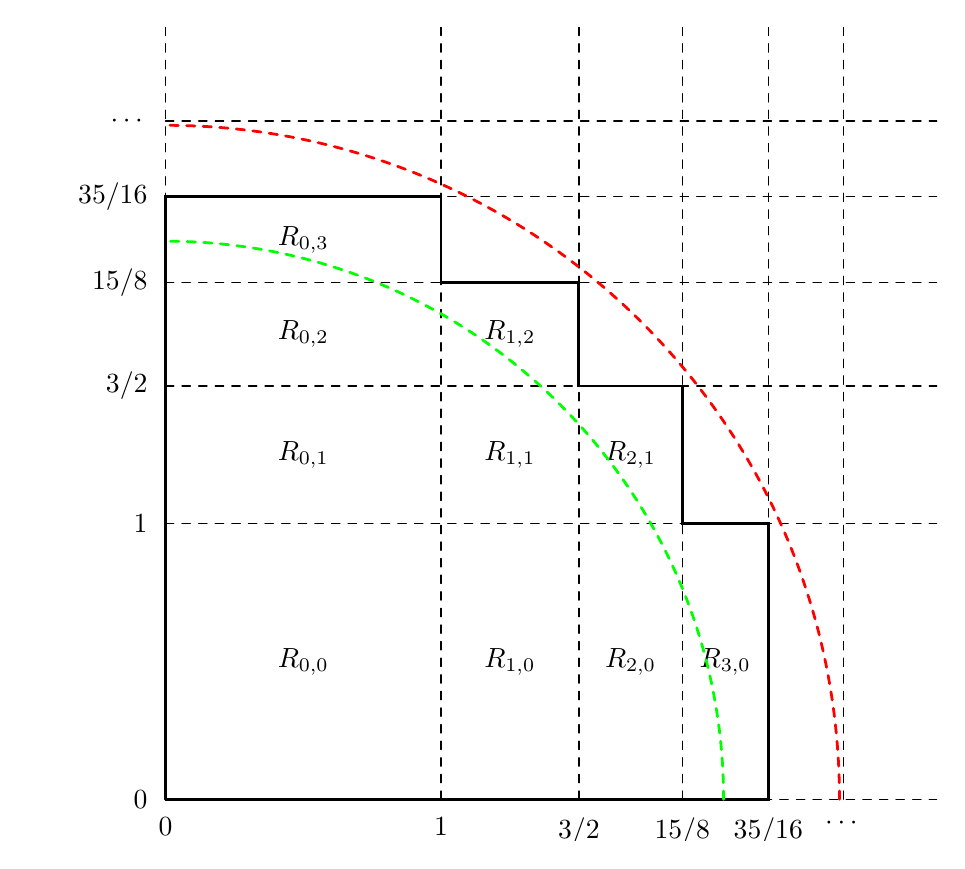
\begin{tikzpicture}[cap=round,scale=3.5]
\def\a{0}
\def\b{1}
\def\c{1.5}
\def\d{1.875}
\def\e{2.1875}
\def\f{2.4609375}
\def\ab{0.5}
\def\bc{1.25}
\def\cd{1.6875}
\def\de{2.03125}
\clip(-0.5,-0.15) rectangle (2.8,2.8);
\def\mylist{0/0,1/1,1.5/{3/2},1.875/{15/8},2.1875/{35/16},2.4609375/{$\cdots$}}
\foreach \xx/\label in \mylist{
	\draw [line width=0.5pt,dashed] (0,\xx) -- (10,\xx);
	\draw [line width=0.5pt,dashed] (\xx,0) -- (\xx,10);
	\draw (\xx,-0.03) node[anchor=north] {\label};
	\draw (-0.03,\xx) node[anchor=east] {\label};
}
\draw [line width=1pt] (\a,\a) -- (\a,\e) -- (\b,\e) -- (\b,\d) -- (\c,\d) -- (\c,\c) -- (\d,\c) -- (\d,\b) -- (\e,\b) -- (\e,\a) -- (\a,\a) ;
\draw (\ab,\ab) node {$R_{0,0}$};
\draw (\ab,\bc) node {$R_{0,1}$};
\draw (\ab,\cd) node {$R_{0,2}$};
\draw (\ab,\de) node {$R_{0,3}$};
\draw (\bc,\ab) node {$R_{1,0}$};
\draw (\bc,\bc) node {$R_{1,1}$};
\draw (\bc,\cd) node {$R_{1,2}$};
\draw (\cd,\ab) node {$R_{2,0}$};
\draw (\cd,\bc) node {$R_{2,1}$};
\draw (\de,\ab) node {$R_{3,0}$};
\def\xx{2.4457}
\def\yy{2.0252}
\draw[dashed,red,line width=1pt] (\xx,0) arc [start angle=0, end angle=90, radius=\xx];
\draw[dashed,green,line width=1pt] (\yy,0) arc [start angle=0, end angle=90, radius=\yy];
\end{tikzpicture}
\end{figure*}

多边形 $P_n $ 往外凸的点是集合 $\{ (s_i, s_j)\ |\ \ i+j=n+1,\ 1\le i,j \le n \}$. 这些点到原点的距离是 $ \sqrt{s_i^2+s_j^2} $. 根据前面推出的 $ s_i $ 与 $ o_n $ 的大小关系有
\[ \sqrt{s_i^2+s_j^2} \le \sqrt{\frac{2i+2j}{o_n}} = \sqrt{\frac{2(n+1)}{o_n}} .\]

类似的, 这个多边形向内凹的点是集合  $\{ (s_k, s_l)\ |\ \ k+l=n,\ 0\le k,l \le n \}$. 根据前面推出的 $ s_i $ 与 $ e_n $ 的大小关系有
\[ \sqrt{s_k^2+s_l^2} \ge \sqrt{\frac{2k+2l-2}{e_n}} = \sqrt{\frac{2(n-1)}{e_n}} .\]

也就是说, 多边形 $ P_n $ 的边被夹在半径为 $ \sqrt{2(n-1)/e_n} $ 和 $ \sqrt{2(n+1)/o_n} $ 的两个四分之一圆之间. 上面的图中也画出了这两个圆. 于是他们的面积满足关系
\[ \pi\cdot\frac{n-1}{2e_n} \le n \le \pi\cdot\frac{n+1}{2o_n} ,\]
所以 \[ \frac{(n-1)\pi}{2n} \le e_n < o_n \le \frac{(n+1)\pi}{2n} .\]
当 $ n  \rightarrow  \infty $ 时, 不等式两边都是 $ \pi/2 $, 而 $ e_n $ 和 $ o_n $ 也都是 Wallis 乘积. 命题得证.

\newpage
%------------------------------------------------------------------------------%
\section{欧拉的奇迹}
本小节参考 William Dunham 所著的 "Euler's Miracle" 一文. 该文分析了一种交错的调和级数.
虽然调和级数是发散的, 欧拉改变了调和级数的某些项的符号, 得到了收敛的结果, 并且收敛值正好是 $ \pi $.

\subsection{欧拉交错级数}

这里讨论的级数定义如下:
\begin{align*}
E &= 1 + \frac{1}{2} + \frac{1}{3} + \frac{1}{4} - \frac{1}{5} + \frac{1}{6} + \frac{1}{7} + \frac{1}{8} + \frac{1}{9} - \frac{1}{10} \\ 
& + \frac{1}{11} + \frac{1}{12} - \frac{1}{13} + \frac{1}{14} - \frac{1}{15} + \frac{1}{16} - \frac{1}{17} + \frac{1}{18} + \frac{1}{19} - \frac{1}{20} \\
& + \frac{1}{21} + \frac{1}{22} + \frac{1}{23} + \frac{1}{24} + \frac{1}{25} - \frac{1}{26} + \frac{1}{27} + \frac{1}{28} - \frac{1}{29} - \frac{1}{30} \\
& + \frac{1}{31} + \frac{1}{32} + \frac{1}{33} - \frac{1}{34} - \frac{1}{35} + \cdots
\end{align*}

改变符号的规则为: 对于任意正整数 $ n $, 如果 $n$ 含有奇数个形如 $ 4k + 1$ 的素因子(包含重复的), 那么 $\dfrac{1}{n} $ 的符号就是负的.

为了证明这个结论, 欧拉使用了 4 条已有的结论. 

\begin{enumerate}
\item Leibniz 级数: 
\[ 1-\frac{1}{3}+\frac{1}{5}-\frac{1}{7} + \cdots =\frac{\pi}{4} \]
\item 巴塞尔问题: 
\[ 1+\frac{1}{2^2}+\frac{1}{3^2}+\cdots = \frac{\pi^2}{6} \]
\item 几何级数的求和:
\[ 1 + a + a^2 + a^3 + \cdots = \frac{1}{1-a}, \quad -1 < a < 1 \]
\item 算术基本定理或正整数唯一分解定理: 任何一个大于1的自然数, 如果它不为质数,那么它可以唯一分解成有限个质数的乘积.
\end{enumerate}

\subsection{Leibniz 级数的乘积形式}

欧拉的证明过程是先将 Leibniz 级数公式与它自身的 $\dfrac{1}{3}$ 相加:
\begin{align*}
\frac{\pi}{4} &= 1-\frac{1}{3}+\frac{1}{5}-\frac{1}{7} +\frac{1}{9} - \frac{1}{11} + \frac{1}{13} - \frac{1}{15} + \frac{1}{17} - \frac{1}{19} + \frac{1}{21} - \frac{1}{23} +\cdots \\
\frac{1}{3}\cdot\frac{\pi}{4} &= \frac{1}{3}-\frac{1}{9}+\frac{1}{15}-\frac{1}{21}+\cdots \\
\frac{\pi}{4}(1+\frac{1}{3})&=1+\frac{1}{5}-\frac{1}{7}-\frac{1}{11}+\frac{1}{13}+\frac{1}{17}-\frac{1}{19}-\frac{1}{23}+\cdots
\end{align*}

最后一个式子里, 分母为 3 的倍数的项被消去了. 接着再减去上面最后一个等式的 $\dfrac{1}{5}$, 得到:
\begin{align*}
\frac{\pi}{4}(1+\frac{1}{3})&=1+\frac{1}{5}-\frac{1}{7}-\frac{1}{11}+\frac{1}{13}+\frac{1}{17}-\frac{1}{19}-\frac{1}{23}+\cdots\\
\frac{1}{5}\cdot\frac{\pi}{4}(1+\frac{1}{3}) &= \frac{1}{5} + \frac{1}{25} - \frac{1}{35} - \cdots \\
\frac{\pi}{4}(1+\frac{1}{3})(1-\frac{1}{5})&=1-\frac{1}{7}-\frac{1}{11}+\frac{1}{13}+\frac{1}{17}-\frac{1}{19}-\frac{1}{23}+\cdots
\end{align*}

这里, 分母是 3 和 5 的倍数的项都没了. 如此, 再加上上面式子的 $\dfrac{1}{7}$:
\[  
\frac{\pi}{4}(1+\frac{1}{3})(1-\frac{1}{5})(1+\frac{1}{7}) = 1- \frac{1}{11}+\frac{1}{13}+\frac{1}{17}-\frac{1}{19} - \frac{1}{23} + \cdots
\]

以此类推, 每一步等式右边开头都是 $ 1\pm\dfrac{1}{p} $ 的形式, 其中 $ p $ 是一个质数. 无限重复下去, 根据 $\dfrac{1}{p}$ 在 Leibniz 级数中的正负号决定下一步乘上的是 $(1+\dfrac{1}{p})$ 还是 $(1-\dfrac{1}{p})$. Leibniz 级数中的正负号规律很容易看出来, $\dfrac{1}{4k+1}$ 是加号, $\dfrac{1}{4k+3}$ 是减号. 于是, 将上面的过程无限重复, 将得到: 
\[
\frac{\pi}{4}(1+\frac{1}{3})(1-\frac{1}{5})(1+\frac{1}{7})(1+\frac{1}{11})(1-\frac{1}{13})(1-\frac{1}{17})(1+\frac{1}{19}) \cdots = 1
\] 
或者写成:
\[
(1+\frac{1}{3})(1-\frac{1}{5})(1+\frac{1}{7})(1+\frac{1}{11})(1-\frac{1}{13})(1-\frac{1}{17})(1+\frac{1}{19}) \cdots = \frac{4}{\pi}
\]

如此就把求和形式的 Leibniz 级数转成了乘积形式.

\subsection{巴塞尔问题的乘积形式}
考虑下面的分式, 分母中各项里的分数的分母包含了所有质数:
\[
Q = \frac{1}{(1+\frac{1}{2})(1-\frac{1}{2})(1+\frac{1}{3})(1-\frac{1}{3})(1+\frac{1}{5})(1-\frac{1}{5})(1+\frac{1}{7})(1-\frac{1}{7})(1+\frac{1}{11})(1-\frac{1}{11})\cdots}
\]

欧拉将它的相邻项两两结合, 并使用几何级数展开:
\begin{align*}
Q &= \frac{1}{1-\frac{1}{4}}\cdot\frac{1}{1-\frac{1}{9}}\cdot\frac{1}{1-\frac{1}{25}}\cdot\frac{1}{1-\frac{1}{49}}\cdot\frac{1}{1-\frac{1}{121}}\cdot\frac{1}{1-\frac{1}{169}}\cdot\cdots \\
 &= \left(1+\frac{1}{4}+\frac{1}{4^2}+\cdots\right)\left(1+\frac{1}{9}+\frac{1}{9^2}+\cdots\right)\left(1+\frac{1}{25}+\cdots\right)\left(1+\frac{1}{49}+\cdots\right)\cdots
\end{align*}

可以断言, 巴塞尔问题中的任意一项 $ \dfrac{1}{N^2}$会在这个乘积中出现且仅出现一次. 这是因为 $ N $ 可以被唯一地表示成质数的乘积: $ N = \prod p_i^{k_i} $, 其中 $ p_i $ 是第 $ i $ 个质数, $ k_i $ 是自然数.
则 $ N^2 = \prod (p_i^2)^{k_i} $. 每个 $ N $ 对应一组 $\{k_i\}$ 的序列, 且该序列非零项个数是有限的. 而这样的序列一一对应了上面乘积展开式中的一项. 于是
\[Q = 1 + \frac{1}{4} + \frac{1}{9} + \frac{1}{16} + \cdots = \frac{\pi^2}{6} .\]

或者写成
\[(1+\frac{1}{2})(1-\frac{1}{2})(1+\frac{1}{3})(1-\frac{1}{3})(1+\frac{1}{5})(1-\frac{1}{5})(1+\frac{1}{7})(1-\frac{1}{7})\cdots= \frac{1}{Q} = \frac{6}{\pi^2}\]

左边是 $(1\pm\frac{1}{p})$ 形式的乘积, $p$ 为质数.

\subsection{证明结论}

得到了前述的 Leibniz 级数和巴塞尔问题的乘积形式后, 将二者相除, 在乘以 $ \dfrac{3}{2} $, 得到
\begin{align*}
 \pi &= \frac{3}{2}\left[\frac{4/\pi}{6/\pi^2}\right] \\
&=  \frac{3}{2}\left[\frac{(1+\frac{1}{3})(1-\frac{1}{5})(1+\frac{1}{7})(1+\frac{1}{11})(1-\frac{1}{13})(1-\frac{1}{17})(1+\frac{1}{19})\cdots}{(1+\frac{1}{2})(1-\frac{1}{2})(1+\frac{1}{3})(1-\frac{1}{3})(1+\frac{1}{5})(1-\frac{1}{5})(1+\frac{1}{7})(1-\frac{1}{7})\cdots}\right] \\
&= \frac{1}{1-\frac{1}{2}}\cdot\frac{1}{1-\frac{1}{3}}\cdot\frac{1}{1+\frac{1}{5}}\cdot\frac{1}{1-\frac{1}{7}}\cdot\frac{1}{1-\frac{1}{11}}\cdot\frac{1}{1+\frac{1}{13}}\cdot\frac{1}{1+\frac{1}{17}}\cdot\frac{1}{1-\frac{1}{19}}\cdots
\end{align*}
可以发现, 最后的式子中, 对于奇素数 $ p $, 如果 $p$ 是 $4k+1$ 的形式, 则对应 $\left(1+\dfrac{1}{p}\right)^{-1}$ 的项; 如果 $p$ 是 $4k+3$ 的形式, 则对应 $\left(1-\dfrac{1}{p}\right)^{-1}$ 的项.

继续应用几何级数展开, 得到
\begin{align*}
\pi = & \left(1+\frac{1}{2}+\frac{1}{2^2}+\cdots\right)\times\left(1+\frac{1}{3}+\frac{1}{3^2}+\cdots\right)\times\left(1-\frac{1}{5}+\frac{1}{5^2}-\cdots\right)\times\\
& \left(1+\frac{1}{7}+\frac{1}{7^2}+\cdots\right)\times\left(1+\frac{1}{11}+\frac{1}{11^2}+\cdots\right)\times\left(1-\frac{1}{13}+\frac{1}{13^2}-\cdots\right)\times\cdots
\end{align*}

这些乘积中的每一个级数, 有些全是加号, 有些是加减号交错的. 将乘积展开就能得到调和级数的每一项, 并且是一一对应的. 如果分母恰有奇数个 $4k+1$ 形式的素因数, 在欧拉交错级数中就是减号. 

\newpage
%------------------------------------------------------------------------------%
\section{二项式定理的推广}
\subsection{杨辉三角的扩展}
二项式定理: \[(1+x)^n = \sum_{k=0}^{n}{C_n^k}x^k \].
其中组合数 $ C_n^k $ 使用下面的方式计算: \[ C_n^k = \frac{n!}{k!(n-k)!} = \frac{n\cdot(n-1)\cdots 2\cdot 1}{k!\cdot(n-k)(n-k-1)\cdots 2\cdot 1} = \frac{n\cdot(n-1)\cdots (n-k+1)}{k!}\]
因为 $ k $ 是自然数, 当 $ n >= 0 $ 时, 对于 $ k \ge n $, 分子中总是会存在 $ (n-n) $ 的一项. 所以展开式只有有限项.

如果 $ n < 0 $ 又如何? 多项式展开系数可以通过所谓的杨辉三角递推地求出来, 杨辉三角一般写成下面的样子:
%\begin{figure*}[htpb]
\begin{center}
\begin{tabular}{>{$n=}l<{$\hspace{12pt}}*{13}{c}}
0 &1&&&&&&&&&&&&\\
1 &1&&1&&&&&&&&&&\\
2 &1&&2&&1&&&&&&&&\\
3 &1&&3&&3&&1&&&&&&\\
4 &1&&4&&6&&4&&1&&&&\\
5 &1&&5&&10&&10&&5&&1&&\\
6 &1&&6&&15&&20&&15&&6&&1
\end{tabular}
\end{center}
%\end{figure*}
对于任意 $ n $, 
\[ (1+x)^{n+1} = (1+x)(1+x)^n = \sum_{k=0}^{n}{C_n^k}x^k + x\sum_{k=0}^{n}{C_n^k}x^k .\]
容易得到 $ (1+x)^{n+1} $ 的 $ k $ 次幂系数是 $ (1+x)^n $ 的 $ k $ 次幂 与 $ k - 1 $ 次幂的系数之和, 或 $ C_{n+1}^k = C_n^{k-1} + C_n^k $. 这也就是杨辉三角相邻两层之间的递推关系.

注意这个关系的推出并没有限制 $ n \ge 0 $. 我们可以尝试对杨辉三角往上做扩充. 把每行的空位填上 $ 0 $, 并且上下两层之间仍然满足递推关系:
\begin{center}
\begin{tabular}{>{$n=}l<{$\hspace{12pt}}*{13}{c}}
-4&1&&-4&&10&&-20&&35&&-56&&84\\
-3&1&&-3&&6&&-10&&15&&-21&&28\\
-2&1&&-2&&3&&-4&&5&&-6&&7\\
-1&1&&-1&&1&&-1&&1&&-1&&1\\
0 &1&&0&&0&&0&&0&&0&&0\\
1 &1&&1&&0&&0&&0&&0&&0\\
2 &1&&2&&1&&0&&0&&0&&0\\
3 &1&&3&&3&&1&&0&&0&&0\\
4 &1&&4&&6&&4&&1&&0&&0\\
5 &1&&5&&10&&10&&5&&1&&0\\
6 &1&&6&&15&&20&&15&&6&&1
\end{tabular}
\end{center}
于是有下面的级数展开, 可以用泰勒级数验证其正确性:
\begin{align*}
(1+x)^{-1} &= 1-x+x^2-x^3+x^4-x^5+\cdots \\
(1+x)^{-2} &= 1-2x+3x^2-4x^3+5x^4-6x^5+\cdots \\
\cdots
\end{align*}

\subsection{分数次幂}
当 $ n $ 不再是整数时, 二项式定理仍然成立. 可以用泰勒级数证明. 例如, 
\[ (1+x)^{\frac{1}{2}} = 1 + \frac{1}{2}x + \frac{1}{2!}\cdot\frac{1}{2}\cdot(\frac{1}{2}-1)x^2+ \frac{1}{3!}\cdot\frac{1}{2}\cdot(\frac{1}{2}-1)\cdot(\frac{1}{2}-2)x^3+\cdots \]

杨辉三角的递推关系也成立. 这意味着我们可以从 $ (1+x) $ 的 $ n $ 次幂展开系数推出 $ n + 1 $, $ n - 1 $, $ n + 2 $, $ n - 2 $ 等等次幂的展开系数. 

下面介绍的两个应用都巧妙的利用了 $ (1+x) ^\frac{1}{2} $ 的多项式展开.

\subsection{速算开方}
以计算 $ \sqrt{3} $ 为例, 取 $ x = -\dfrac{1}{4} $, 有
\begin{align*}
\sqrt{3} &= \sqrt{4(1-\frac{1}{4})} \\
			&= 2(1-\frac{1}{4})^\frac{1}{2}\\
			&= 2\left( 1+\frac{1}{2}(-\frac{1}{4}) + \frac{1}{2!}\frac{1}{2}(-\frac{1}{2})(-\frac{1}{4})^2 + \cdots \right)
\end{align*}

\subsection{牛顿的速算 \texorpdfstring{$\pi$}{pi} 的算法}
单位圆的方程为 $ x^2 + y^2 = 1 $, 考虑用积分求第一象限的1/4圆 $ y = \sqrt{1-x^2} $ 的面积:
\begin{align*}
\frac{\pi}{4} &= \int_0^1{(1-x^2)^\frac{1}{2} dx} \\
				&=\int_0^1\left[1-\frac{1}{2}x^2-\frac{1}{8}x^4-\frac{1}{16}x^6-\frac{5}{128}x^8-\cdots\right] dx \\
\pi &= 4\left[x - \frac{1}{6}x^3 - \frac{1}{40}x^5 - \frac{1}{112}x^7 - \frac{5}{1152}x^9 - \cdots \right]^1_0 \\
	&= 4\left[1-\frac{1}{6} - \frac{1}{40} - \frac{1}{112} - \frac{5}{1152} - \cdots \right]
\end{align*}
这样得出来的结果收敛速度不够快, 如果积分上限是 $ \frac{1}{2} $, 那么余项会以指数的速度缩小.
\begin{figure*}[htbp]
\centering
\definecolor{wrwrwr}{rgb}{0.3803921568627451,0.3803921568627451,0.3803921568627451}
\definecolor{rvwvcq}{rgb}{0.08235294117647059,0.396078431372549,0.7529411764705882}
\subfigure{
\begin{minipage}[b]{0.48\linewidth}
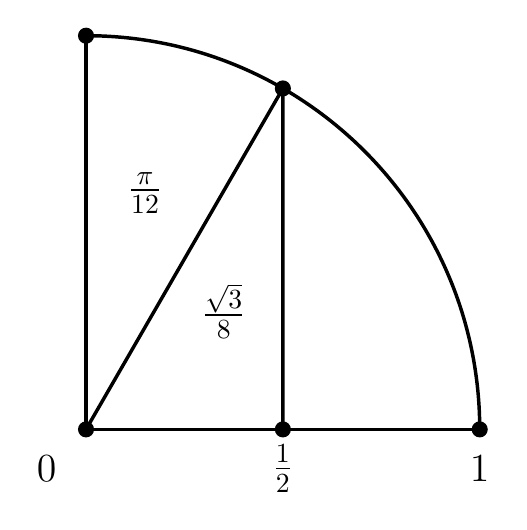
\begin{tikzpicture}[scale=5]
\coordinate[] (O) at (0.0,0.0);
\coordinate[] (A) at (1.0,0.0);
\coordinate[] (B) at (0.0,1.0);
\coordinate[] (C) at (0.5,0.866);
\coordinate[] (D) at (0.5,0.0);
\draw[line width=1.25pt] (A) -- (O) -- (B);
\draw[line width=1.25pt] (A) arc (0:90:1);
\draw[line width=1.25pt] (O) -- (C) -- (D);
\foreach \p in {O,A,B,C,D}
	\fill[fill=black,draw=black,thick] (\p) circle (0.5pt);
\draw[font=\Large] (-0.1, -0.1) node {$0$};
\draw[font=\Large] (1.0, -0.1) node {$1$};
\draw[font=\Large] (0.5, -0.1) node {$\frac{1}{2}$};
\draw[font=\Large] (0.15, 0.6) node {$\frac{\pi}{12}$};
\draw[font=\Large] (0.35, 0.3) node {$\frac{\sqrt{3}}{8}$};
\end{tikzpicture}
\end{minipage}}
\subfigure{
\begin{minipage}[b]{0.48\linewidth}
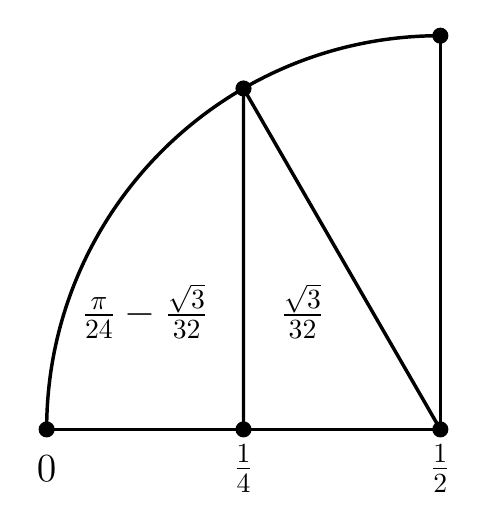
\begin{tikzpicture}[scale=5]
\coordinate[] (O) at (0.0,0.0);
\coordinate[] (A) at (1.0,0.0);
\coordinate[] (B) at (1.0,1.0);
\coordinate[] (C) at (0.5,0.866);
\coordinate[] (D) at (0.5,0.0);
\draw[line width=1.25pt] (O) -- (A) -- (B);
\draw[line width=1.25pt] (B) arc (90:180:1);
\draw[line width=1.25pt] (A) -- (C) -- (D);
\foreach \p in {O,A,B,C,D}
	\fill[fill=black,draw=black,thick] (\p) circle (0.5pt);
\draw[font=\Large] (-0.0, -0.1) node {$0$};
\draw[font=\Large] (1.0, -0.1) node {$\frac{1}{2}$};
\draw[font=\Large] (0.5, -0.1) node {$\frac{1}{4}$};
\draw[font=\Large] (0.25, 0.3) node {$\frac{\pi}{24}- \frac{\sqrt{3}}{32}$ };
\draw[font=\Large] (0.65, 0.3) node {$\frac{\sqrt{3}}{32}$};
\end{tikzpicture}
\end{minipage}}
\end{figure*}

如图所示, 积分区间取 $ [0, \frac{1}{2} ] $ 对应的区域可以划分成一个扇形和一个直角三角形, 扇形面积是 $ \pi/12 $, 三角形面积是 $ \sqrt{3}/8 $. 所以:
\[
\frac{\pi}{12}+\frac{\sqrt{3}}{8} = \int_0^\frac{1}{2}{(1-x^2)^\frac{1}{2} dx} 
\]
\[
\pi = 12\left[ -\frac{\sqrt{3}}{8} + \frac{1}{2}-\frac{1}{6}(\frac{1}{2})^3-\frac{1}{40}(\frac{1}{2})^5 - \frac{1}{112}(\frac{1}{2})^7 - \frac{5}{1152}(\frac{1}{2})^9 - \cdots \right]
\]

另一种减小积分上限的方法是考虑圆的方程是 $ x^2 - x + y^2 = 0 $, 它的圆心在 $ (\dfrac{1}{2}, 0) $, 半径为 $ \dfrac{1}{2} $. 积分区间是 $ [0,\frac{1}{4} ]$, 被积函数是 $ y = \sqrt(x - x^2) $, 面积关系为:
\begin{align*}
\frac{\pi}{24} - \frac{\sqrt{3}}{32} &= \int_0^\frac{1}{4}{x^\frac{1}{2}(1-x)^\frac{1}{2} dx} \\
		&= \int_0^\frac{1}{4}{ x^\frac{1}{2}\left[ 1-\frac{1}{2}x - \frac{1}{8}x^2-\frac{1}{16}x^3-\frac{5}{128}x^4-\cdots \right] dx} \\
		&= \int_0^\frac{1}{4}{ \left[ x^\frac{1}{2}-\frac{1}{2}x^\frac{3}{2}-\frac{1}{8}x^\frac{5}{2}-\frac{1}{16}x^\frac{7}{2}-\frac{5}{128}x^\frac{9}{2}-\cdots \right] dx} \\
		&= \left[ \frac{2}{3}x^\frac{3}{2} - \frac{1}{2}\cdot\frac{2}{5}x^\frac{5}{2}-\frac{1}{8}\cdot\frac{2}{7}x^\frac{7}{2}-\frac{1}{16}\cdot\frac{2}{9}x^\frac{9}{2}-\frac{5}{128}\cdot\frac{2}{11}x^\frac{11}{2} - \cdots \right]_0^\frac{1}{4} \\
\pi &= \frac{3\sqrt{3}}{4}+24\left(\frac{1}{12}-\frac{1}{5\cdot 2^5}-\frac{1}{28\cdot 2^7} -\frac{1}{72\cdot 2^9} - \frac{5}{704\cdot 2^{11}} -\cdots \right) 
\end{align*}


\newpage
%------------------------------------------------------------------------------%
\section{阿基米德如何计算球的表面积}

核心思想在于将球的表面与一个正好包住球的圆柱体侧面建立联系, 假设球的半径为 $R$, 则圆柱的底面半径为 $R$, 高为 $2R$, 侧面积正好是 $2\pi R\cdot 2R=4\pi R^2$, 如下图所示:
\begin{figure}[htbp]
\centering

\begin{minipage}[t]{0.35\linewidth}
\centering
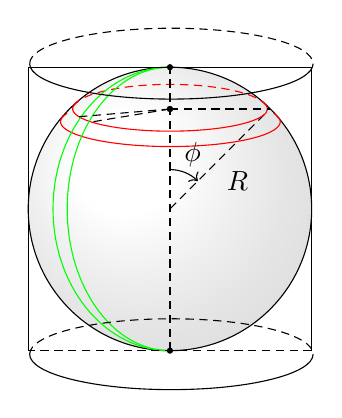
\begin{tikzpicture}[scale=0.9]
  \coordinate (O) at (0,0);
\coordinate (1) at (0,1.41);
\coordinate (2) at (0,2);
\coordinate (3) at (1.41,1.41);
  % ball background color
  \shade[ball color = white, opacity = 0.2] (0,0) circle [radius = 2cm];
  % ball
  \draw (O) circle [radius=2cm];
  % label of ball center point
  % \filldraw (O) circle (1pt) node[below] {$O$};
  % radius
%  \draw[densely dashed] (O) -- (-1.33,1.33);
  \draw[densely dashed] (1.33,1.33) to [edge label = $R$] (O);
  % cut of ball surface
  %\draw[red] (-1.35,1.47) arc [start angle = 140, end angle = 40, x radius = 17.6mm, y radius = 14.75mm];	% top
  \draw[red, densely dashed] (-1.36,1.46) arc [start angle = 170, end angle = 10, x radius = 13.8mm, y radius = 3.6mm];
  \draw[red] (-1.29,1.52) arc [start angle=-200, end angle = 20, x radius = 13.75mm, y radius = 3.15mm];
  \draw[red] (-1.45,1.35) arc [start angle=-200, end angle = 20, x radius = 15.5mm, y radius = 3.5mm];
\filldraw (1) circle (1pt);
 \draw[green] (0,2) arc [start angle=90, end angle =-90, x radius = -16.5mm, y radius = 20mm];
 \draw[green] (0,2) arc [start angle=90, end angle =-90, x radius = -14.5mm, y radius = 20mm];
\draw[densely dashed] (1) to (-1.3, 1.3);
\draw[densely dashed] (1) to (-1.15, 1.22);
\filldraw (1) circle (1pt);
\draw[densely dashed] (1) to (3);
\draw[densely dashed] (0,-2) -- (2);
\draw
    (0,2) coordinate (a)
    (0,0) coordinate (b)
    (1.41,1.41) coordinate (c)
    pic["$\phi$", draw,<-, angle eccentricity=1.5, angle radius=0.5cm]
    {angle=c--b--a};
%cylinder
\draw[] (-2, -2) -- (-2,2) -- (2,2) -- (2,-2);
\draw[densely dashed] (2, -2) -- (-2,-2);
\draw[densely dashed] (-1.98,-2.05) arc [start angle = 180, end angle = 0, x radius = 20.0mm, y radius = 5.0mm];
\draw[] (-1.98,-2.05) arc [start angle=-180, end angle = 0, x radius = 20.0mm, y radius = 5.0mm];
\draw[densely dashed] (-1.98,2.05) arc [start angle = 180, end angle = 0, x radius = 20.0mm, y radius = 5.0mm];
\draw[] (-1.98,2.05) arc [start angle=-180, end angle = 0, x radius = 20.0mm, y radius = 5.0mm];
\filldraw (0,-2) circle (1pt);
\filldraw (0,2) circle (1pt);
\end{tikzpicture}
\end{minipage}
\begin{minipage}[t]{0.59\linewidth}
\centering
\begin{tikzpicture}[scale=0.9]
\draw[] (-4,2) -- (4,2) -- (4,-2);
\draw[] (-4,-2) to [edge label = $2 R$] (-4, 2);
\draw[] (4,-2) to [edge label = $2\pi R$] (-4, -2);
\draw[red] (-4,1.41) -- (4,1.41);
\draw[red] (-4,1.2) -- (4,1.2);
\draw[green] (-2.2,-2) to  (-2.2, 2);
\draw[green] (-2.0,-2) to  (-2.0, 2);
\end{tikzpicture}
\end{minipage}
\end{figure}

用球面坐标系, $(\theta, \phi)$ 表示经纬度, $\theta \in [0, 2\pi), \phi \in [0,\pi]$, 且 $\phi=0$ 表示北极点. 考虑点 $(\theta, \phi)$ 处的面积微元, 在经线方向上是 $R\sin\phi\ \mathrm{d}\theta$, 在纬线方向上是 $R\ \mathrm{d}\phi$, 于是微元为 $\mathrm{d}s = R^2\sin\phi\ \mathrm{d}\theta\ \mathrm{d}\phi$.

再假想有一个光源, 能在 $z$ 轴上各处向四面八方发射光线, 考虑上述面积微元在圆柱侧面的投影. 
经线方向是将半径为 $r=R\sin\phi$, 角度为 $\mathrm{d}\theta$ 的一段圆弧投影到半径为 $R$ 的圆弧上, 所以长度为 $R\ \mathrm{d}\theta$. 
纬线方向是将半径为 $R$, 角度为 $\mathrm{d}\phi$ 的一段圆弧投影到 $z$ 轴上, 而这段圆弧的法向与 $z$ 轴的夹角为 $\phi$, 于是投影的长度为 $R\ \mathrm{d}\phi\cdot\sin\phi$. 
两个方向上乘起来得到投影之后的面积微元仍然是 $\mathrm{d}S = R^2\sin\phi\ \mathrm{d}\theta\ \mathrm{d}\phi$. 说明投影保持了面积大小不变, 所以圆柱侧面积和球表面积相等.

\begin{figure}[htbp]
\centering
\begin{minipage}[t]{0.48\linewidth}
\centering
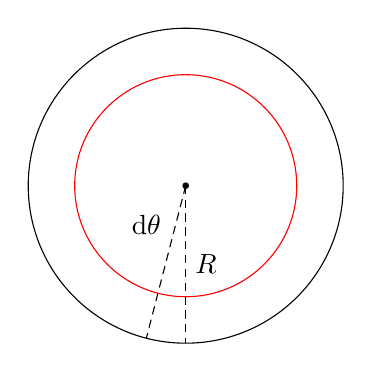
\begin{tikzpicture}[]
  \coordinate (O) at (0,0);
\coordinate (1) at (0,1.41);
\coordinate (2) at (0,2);
\coordinate (3) at (1.41,1.41);
  \draw (O) circle [radius=2cm];
\filldraw (0,0) circle (1pt);
\draw[densely dashed] (0,0) to [edge label = $R$] (0,-2);
\draw[densely dashed] (0,0) to (-0.5,-1.936);
%\draw[red] (0, -1.41) arc [start angle = -90, end angle = -105, radius = 1.41];
\draw[red]  (O) circle [radius=1.41cm];
\draw (-0.5,-0.5) node {$\mathrm{d}\theta$};
\end{tikzpicture}
\end{minipage}
\begin{minipage}[t]{0.48\linewidth}
\centering
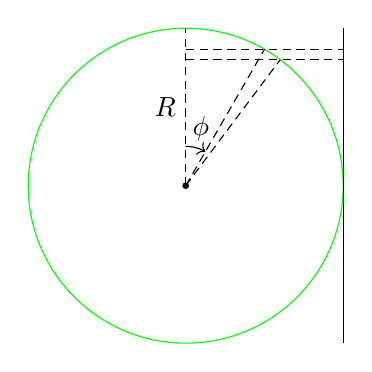
\begin{tikzpicture}[]
  \coordinate (O) at (0,0);
\coordinate (1) at (0,1.41);
\coordinate (2) at (0,2);
\coordinate (3) at (1.41,1.41);
  \draw[green] (O) circle [radius=2cm];
\filldraw (0,0) circle (1pt);
\draw[densely dashed] (0,0) to [edge label = $R$] (0,2);
\draw[densely dashed] (0,0) to (1,1.732);
\draw[densely dashed] (0,0) to (1.2,1.6);
\draw
    (0,2) coordinate (a)
    (0,0) coordinate (b)
    (1.0,1.732) coordinate (c)
    pic["$\phi$", draw,<-, angle eccentricity=1.5, angle radius=0.5cm]
    {angle=c--b--a};
\draw (2,-2) to (2,2);
\draw [densely dashed](0,1.732) to (2,1.732);
\draw [densely dashed](0,1.6) to (2,1.6);
\end{tikzpicture}
\end{minipage}
\end{figure}

上图示意了投影的过程. 左边是纬线的投影, 从 $z+$ 方向俯视, 红线代表纬线. 一段纬线上的圆弧, 投射到外层圆柱上之后, 长度拉伸了 $\sin\phi$ 倍. 上图右边是经线的投影, 视线垂直于经线和 $z$ 轴所在平面. 经线上的一小段圆弧的切线方向与 $xy$ 平面夹角是 $\phi$, 投影到 $z$ 轴或圆柱侧面上时, 缩短的比例为 $\sin\phi$. 纬线上的拉伸和经线上的缩短正好抵消了.

\newpage
%------------------------------------------------------------------------------%
\section{Fibonacci 数列}

一般 Fibonacci 数列定义如下: $x_0 = 0, x_1 = 1, x_{n+1} = x_{n} + x_{n-1} $.

\subsection{通项公式: 初等解法}

我们尝试将递推关系凑出下面的形式: 
\[ x_{n+1} + ax_n = b(x_n+ax_{n-1}) .\]
从而可以令 $ y_n = x_{n+1} + ax_n $, 然后求出 $ y_n $, 进而求出 $ x_n $.

比较系数可以得到: $ b - a = 1 $, $ ab = 1 $.于是可以解出 $ a = \dfrac{\sqrt{5}-1}{2}$, $ b = \dfrac{\sqrt{5}+1}{2}$.
进一步, $y_0 = x_1+ax_0 = 1 $, $ y_n = b^n $.
\begin{align*} 
x_{n+1}+ax_n &= b^n \\
ax_n+a^2x_{n-1} &= ab^{n-1} \\
\cdots & \\
a^{n-1}x_2 + a^{n}x_1 &= a^{n-1}b \\
a^{n}x_1 + a^{n+1}x_0 &= a^nb^{0}
\end{align*}

错位相减得 $ x_{n+1} = b^n - ab^{n-1} + a^2b^{n-2} - \cdots + (-1)^na^n $. 这是一个等比数列之和, 注意到 $ a $ 和 $ b $ 互为倒数, 公比是 $ -ab^{-1}=-a^2 $, 这个的和其实就是:
\[ x_{n+1} = \frac{b^n-(-a)^n(-a^2)}{1-(-a^2)} = \frac{b^{n+1}-(-a)^{n+1}}{b+a} = \frac{b^{n+1}-(-a)^{n+1}}{\sqrt{5}}.\]

所以通项公式是: 
\[ x_n = \frac{1}{\sqrt{5}}\left[ \left(\frac{\sqrt{5}+1}{2}\right)^n - \left(\frac{1-\sqrt{5}}{2}\right)^n \right] .\]

\subsection{通项公式: 矩阵解法}

Fibonacci 数列的递推关系可以写成矩阵的形式:
\[
\begin{bmatrix}
x_{n+1} \\
x_n 
\end{bmatrix} = 
\begin{bmatrix}
& 1 & 1 & \\
& 1 & 0 & 
\end{bmatrix}
\begin{bmatrix}
x_n \\
x_{n-1}
\end{bmatrix}
=F \begin{bmatrix}
x_n \\
x_{n-1}
\end{bmatrix}
=\cdots
=F^{n} \begin{bmatrix}
x_1 \\
x_0
\end{bmatrix}
\]
将矩阵 $ F $ 做对角化分解: $ F = P^{-1} \Lambda P $. 其中 
\[ \Lambda = \begin{bmatrix} -a & 0 \\ 0 & b \end{bmatrix} , P = \frac{1}{\sqrt{5}}\begin{bmatrix} -1 & b \\ 1 & a \end{bmatrix}, P^{-1} = \begin{bmatrix} -a & b \\ 1 & 1 \end{bmatrix} .\]
则 
\begin{align*}
F^{n} &= P^{-1}\Lambda^{n} P \\
% &= \frac{1}{\sqrt{5}}\begin{bmatrix}
%-a & b \\ 1 & 1
%\end{bmatrix}
%\begin{bmatrix}
%(-a)^{n} & 0 \\ 0 & b^{n}
%\end{bmatrix}
%\begin{bmatrix}
%-1 & b \\ 1 & a
%\end{bmatrix} \\
 &= \frac{1}{\sqrt{5}}\begin{bmatrix}
b^{n+1} - (-a)^{n+1} & ab^{n+1}+b(-a)^{n+1} \\b^n - (-a)^n & ab^n+b(-a)^n 
\end{bmatrix} 
.\end{align*}
代入 $x_1$ 和 $ x_0$ 的值可以得到通项: $x_n = \dfrac{1}{\sqrt{5}}\left(b^n - (-a)^n\right)$.

\subsection {模的周期}
考虑 Fibonacci 数列关于整数 $m$ 的模, 下面的讨论均是在模 $m$ 的意义下进行. 

先研究相邻两项组成的二元组 $(x_{n+1},x_n)$ 模 $m$ 的余数. 这样的余数二元组最多有 $ m^2 $ 种可能, 所以一定会出现重复的. 不妨令 $(x_{k+1},x_k) \equiv (x_{k+p+1},x_{k+p}) $, 根据上面的矩阵形式的递推关系, 有:
\[
F^k
\begin{bmatrix}
x_{1} \\ x_0
\end{bmatrix}
\equiv  F^{k+p}
\begin{bmatrix}
x_{1} \\ x_0
\end{bmatrix}
\]
而矩阵 $ F $ 是可逆的, 我们把上面等式两边都乘以 $ F^{-k} $, 可知二元组 $(x_1,x_0)$ 经过 $ p $ 次以后又回到了 $(x_1,x_0)$. 

另一个结论是: 如果 $ m = x_p $, 则模 $ m $ 的循环周期是 $ p $. 例如, $ x_4 = 3 $, $ x_{4k} $ 都能被 $ 3 $ 整除.
\begin{table}[h!]
\centering
\begin{tabular}{ c c c c c c c c c c c c c c c c c }
\hline 
$n$ & 0 & 1 & 2 & 3 & 4 & 5 & 6 & 7 & 8 & 9 & 10 & 11 & 12 & 13 & 14 & $\cdots$\\
\hline 
$x_{n}$ & 0 & 1 & 1 & 2 & 3 & 5 & 8 & 13 & 21 & 34 & 55 & 89 & 144 & 233 & 377 & $\cdots$ \\
\hline 
\end{tabular}
\end{table}

这很容易证明. 显然, $ x_p \equiv 0 \pmod{x_p}$, 假设 $ x_{p+1} \equiv r \pmod{x_p} $, 后续序列分别是 $ r, r, 2r, 3r, 5r, \cdots $, 也就是将第一个周期内的序列乘以 $ r $ 再重复一遍, 这样到 $ x_{2p} $ 的时候余数又会回到 $ 0 $. 等等.

\subsection {Arnold 变换}

给一个 $ m\times m $ 的图像, 一次Arnold 变换是将 $ (x,y) $ 处的像素移动到 $ (2x+y, x+y) \bmod{m}$ 处. 重复若干次以后, 图像就会变得杂乱无章. 再继续进行变换, 图像会回到原来的样子. 由 Arnold 提出, 并且用例图片都是猫, 所以又被称为 "猫映射"(cat mapping).

记 $(x, y)$ 在经过 $n$ 次变换后的坐标是 $(x_n,y_n)$, 则
\[
\begin{bmatrix}
x_n \\ y_n
\end{bmatrix}
=\begin{bmatrix}
2 & 1 \\ 1 & 1
\end{bmatrix}^n
\begin{bmatrix}
x_0 \\ y_0
\end{bmatrix} = F^{2n} \begin{bmatrix}
x_0 \\ y_0
\end{bmatrix} \bmod{m}.
\]
由前面的分析可以知道 $F$ 经过循环周期会变成单位阵, 所以 Arnold 变换进行若干次也会得到原图像.

\subsection {1/89}
\begin{align*}
1/89 &= 0.01123595505617977528089887640449\cdots \\
	&= 0.0 \\
	 & + 0.01 \\
	&+ 0.001\\
	&+ 0.0002 \\
	&+ 0.00003\\
	&+ 0.000005\\
	&+ 0.0000008\\
	&+ 0.00000013\\
	&+ 0.000000021\\
	&+ 0.0000000034\\
	&+ 0.00000000055\\
	&+\cdots
\end{align*}

其实就是 $\dfrac{x_n}{10^n}$, 代入通项公式求和就是 $ 10 / 89 $.

\newpage
%------------------------------------------------------------------------------%
\section{Thebault problem}

任意一个四边形, 每边朝外作正方形, 连接相对两个正方形的中心, 得到的两组线段相互垂直且长度相等.
\begin{figure*}[htbp]
\centering
\definecolor{wrwrwr}{rgb}{0.3803921568627451,0.3803921568627451,0.3803921568627451}
\definecolor{rvwvcq}{rgb}{0.08235294117647059,0.396078431372549,0.7529411764705882}
\begin{tikzpicture}[]
\coordinate[] (A) at (-1.88,1.68);
\coordinate[] (B) at (0.6,2.8);
\coordinate[] (C) at (1.56,0.44);
\coordinate[label=below left:$O$] (D) at (-2.14,-0.26);
\coordinate[] (AA) at (-1.2,3.48);
\coordinate[] (CC) at (0.06,-1.76);
\coordinate[] (BB) at (-2.98,0.84);
\coordinate[] (DD) at (2.26,2.1);
\coordinate[] (AAA) at (-2.01,0.71);

\draw[line width=1pt,fill=rvwvcq!10] (A) -- (-3.82,1.94) -- (-4.08,0) -- (D);
\draw[line width=1pt,fill=rvwvcq!10] (B) -- (-0.52,5.28) -- (-3,4.16) -- (A);
\draw[line width=1pt,fill=rvwvcq!10] (C) -- (3.92,1.4) -- (2.96,3.76) -- (B);
\draw[line width=1pt,fill=rvwvcq!10] (D) -- (-1.44,-3.96) -- (2.26,-3.26) -- (C);
% \draw[line width=1pt,arrows = {-Stealth[]}] (D) to [edge label' = $2a$] (A); 
\draw[line width=1pt] (D) to [edge label' = $2a$] (A); 
\draw[line width=1pt] (A) to [edge label' = $2b$] (B);
\draw[line width=1pt] (B) to [edge label' = $2c$] (C);
\draw[line width=1pt] (C) to [edge label = $2d$] (D);

%\draw[densely dashed,line width=1pt] (A) -- (AA)--(B);
%\draw[densely dashed,line width=1pt] (B) -- (DD)--(C);
%\draw[densely dashed,line width=1pt] (C) -- (CC)--(D);
\draw[densely dashed,line width=1pt] (D) -- (BB) -- (AAA);

\draw [line width=1pt,color=wrwrwr] (AA)-- (CC);
\draw [line width=1pt,color=wrwrwr] (BB)-- (DD);

\foreach \p in {AA,BB,CC,DD,A,B,C,D,AAA}
	\fill[fill=black,draw=black,thick] (\p) circle (1.25pt);
\end{tikzpicture}
\end{figure*}

\begin{proof}
假设沿顺时针方向, 四边形四条边对应的向量用复数表示分别是 $ 2a, 2b, 2c, 2d $, 假设 $ 2a $ 的起点为原点. 因为四边形是封闭的, 所以 $ a + b + c + d = 0 $. 

从原点出发, 走 $ a $, 再左转 $ 90\degree $ 后走相同的长度, 可以得到边 $ 2a $ 对应的正方形中心为 \[ P_1 = a + ae^{i\frac{\pi}{2}} = a(1+i). \]
其他正方形的中心分别为 
\begin{align*} 
P_2 &= 2a + b(1+i) \\ 
P_3 &= 2a + 2b + c(1+i) \\
P_4 &= 2a + 2b + 2c + d(1+i).
\end{align*}
连接相对两个正方形中心的线段对应的向量为以下两个复数:
\[ P_3 - P_1 = a + 2b + c + (c-a)i = b - d + (c-a)i, \]
\[ P_4 - P_2 = b + 2c + d + (d-b)i = c - a + (d-b)i. \]

容易发现 $ (P_3 - P_1) = (P_4 - P_2)i $, 所以它们相互垂直, 且长度相等.

\end{proof}

~

\noindent 另一种证明方法:

首先研究复平面上的平移和旋转变换, 用 $ T_v $ 表示平移一个向量 ( 或复数 ) $ v $ 的运算: $ T_v(z) = z + v $, 用 $ R_a^\theta $ 表示绕一点 $ a $ 旋转角度 $ \theta $. 其中绕原点的旋转可以写成 $ R_0^\theta(z) = e^{i\theta}z $.

一般的旋转等价于先把 $ a $ 平移到原点, 再绕原点旋转 $ \theta $, 最后把原点平移回 $ a $.
\[ R_a^\theta(z) = (T_a\circ R_0^\theta \circ T_a^{-1})(z) = e^{i\theta}(z-a)+a = e^{i\theta}z+k .\]
其中 $ k = a(1-e^{i\theta}) $. 也就是说, 任何旋转都可以表示成先绕原点做旋转, 再平移, 即: $ R_a^\theta = (T_k\circ R_0^\theta) $. 反过来也成立, 先绕原点旋转 $ \alpha $ 然后平移 $ v $ 的变换等价于绕某个点旋转同样的角度 $ \alpha $: 
\[ T_v \circ R_0^\alpha=R_c^\alpha ,\]
其中 $ c = v/(1-e^{i\alpha}) $. 类似的可以验证 $ R_0^\theta \circ T_v = R_p^\theta $.

考虑两个旋转的合成: 
\[ (R_b^\phi \circ R_a^\theta) (z) = e^{i(\theta+\phi)}z + v ,\]
其中 $ v = ae^{i\phi}(1-e^{i\theta})+b(1-e^{i\phi}) $.

一般而言, 若 $ \theta + \phi $ 不是 $ 2\pi $ 的整数倍, 则存在一个点 $ c $ 满足整个旋转等价于绕点 $ c $ 转 $ \theta + \phi $ 的角度:
\[ R_b^\phi \circ R_a^\theta = R_c^{(\theta+\phi)}, \]
$ c $ 的值可以由 $ a, b, \theta, \phi $ 表示, 这里略过.

若 $ \theta + \phi $ 是 $ 2\pi $ 的整数倍, 
\[ (R_b^\phi \circ R_a^\theta) (z) = z + (1-e^{i\phi})(b-a) ,\]
它其实是一个平移.

这个结论可以推广到多个旋转的合成, 如果一系列旋转变换的旋转角之和是 $ 2\pi $ 的整数倍, 则变换之后的结果等价于只进行平移.

\begin{figure*}[htbp]
\centering
\definecolor{wrwrwr}{rgb}{0.3803921568627451,0.3803921568627451,0.3803921568627451}
\definecolor{rvwvcq}{rgb}{0.08235294117647059,0.396078431372549,0.7529411764705882}
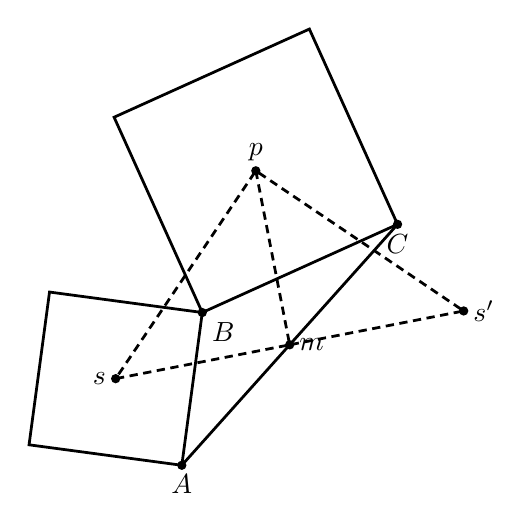
\begin{tikzpicture}[]
\coordinate[label=below right:$B$] (A) at (-1.88,1.68);
\coordinate[label=below:$C$] (B) at (0.6,2.8);
\coordinate[label=below:$A$] (D) at (-2.14,-0.26);
\coordinate[label=right:$m$] (M) at (-0.77,1.27);

\coordinate[label=above:$p$] (AA) at (-1.2,3.48);
\coordinate[label=left:$s$] (BB) at (-2.98,0.84);
\coordinate[label=right:$s'$] (SS) at (1.44, 1.7);
%\coordinate[] (DD) at (2.26,2.1);
% \coordinate[] (AAA) at (-2.01,0.71);

\draw[line width=1pt] (A) -- (-3.82,1.94) -- (-4.08,0) -- (D);
\draw[line width=1pt] (B) -- (-0.52,5.28) -- (-3,4.16) -- (A);
\draw[line width=1pt] (D) -- (A); 
\draw[line width=1pt] (A) -- (B);
%\draw[line width=1pt] (B) to [edge label' = $2c$] (C);
%\draw[line width=1pt] (C) to [edge label = $2d$] (D);

%\draw[densely dashed,line width=1pt] (A) -- (AA)--(B);
%\draw[densely dashed,line width=1pt] (B) -- (DD)--(C);
%\draw[densely dashed,line width=1pt] (C) -- (CC)--(D);
\draw[line width=1pt] (D) -- (B);
\draw[densely dashed,line width=1pt] (AA) -- (M) -- (BB) -- (AA) -- (SS) -- (M) ;

%\draw [line width=1pt,color=wrwrwr] (AA)-- (CC);
%\draw [line width=1pt,color=wrwrwr] (BB)-- (DD);

\foreach \p in {A,B,D,AA,BB,M,SS}
	\fill[fill=black,draw=black,thick] (\p) circle (1.25pt);
\end{tikzpicture}
\end{figure*}
现在回到原问题, 考虑四边形其中两条边 $ AB, BC $ 上的正方形, 正方形的中心为 $ s $ 和 $ p $, 对角线 $ AC $ 的中点为 $ m $, 再考虑三个旋转变换的复合 $ M = R_m^\pi \circ R_p^{(\pi/2)} \circ R_s^{(\pi/2)} $. 

因为三个旋转角度之和为 $ 2\pi $, 由之前的结论知道这其实是一个平移, 为了确定平移量, 考虑点 $ A $ 在这组变换下的结果, 先绕 $ s $ 转 $ 90\degree $ 变换到 $ B $ 点, 再绕 $ p $ 转 $ 90\degree $ 到达 $ C $ 点, 最后绕 $ m $ 转 $ 180\degree $ 回到 $ A $ 点. 

于是可以知道 $ M $ 其实是恒等变换. 从而 $ R_p^{(\pi/2)} \circ R_s^{(\pi/2)} = R_m^{-\pi} = R_m^\pi. $

定义点 $ s' $ 是 $ s $ 绕点 $ m $ 旋转 $ 180\degree $ 的结果: 
\[ s' = R_m^\pi(s) = R_p^{(\pi/2)} \circ R_s^{(\pi/2)}(s) = R_p^{(\pi/2)}(s).\] 
最后一个等号成立是因为 $ s $ 绕 $ s $ 旋转 $ 90\degree $ 仍然是自身.

这说明三角形 $ sps' $ 是等腰三角形, 且 $ \angle sps' $ 是直角. 进一步得到 $ sm $ 和 $ pm $ 垂直且等长.

\begin{figure*}[htbp]
\centering
\definecolor{wrwrwr}{rgb}{0.3803921568627451,0.3803921568627451,0.3803921568627451}
\definecolor{rvwvcq}{rgb}{0.08235294117647059,0.396078431372549,0.7529411764705882}
\begin{tikzpicture}[]
\coordinate[] (A) at (-1.88,1.68);
\coordinate[] (B) at (0.6,2.8);
\coordinate[] (C) at (1.56,0.44);
\coordinate[] (D) at (-2.14,-0.26);
\coordinate[label=above:$p$] (AA) at (-1.2,3.48);
\coordinate[label=below:$r$] (CC) at (0.06,-1.76);
\coordinate[label=left:$s$] (BB) at (-2.98,0.84);
\coordinate[label=right:$q$] (DD) at (2.26,2.1);
\coordinate[label=right:$m$] (M) at (-0.77,1.27);

\draw[line width=1pt] (A) -- (-3.82,1.94) -- (-4.08,0) -- (D);
\draw[line width=1pt] (B) -- (-0.52,5.28) -- (-3,4.16) -- (A);
\draw[line width=1pt] (C) -- (3.92,1.4) -- (2.96,3.76) -- (B);
\draw[line width=1pt] (D) -- (-1.44,-3.96) -- (2.26,-3.26) -- (C);
\draw[line width=1pt] (D) -- (A) -- (B) -- (C) -- cycle; 
\draw [line width=1pt] (B)-- (D);
\draw [line width=1pt,color=wrwrwr] (AA)-- (CC) -- (M) -- cycle;
\draw [line width=1pt,color=wrwrwr] (BB)-- (DD)-- (M) -- cycle;

\foreach \p in {AA,BB,CC,DD,A,B,C,D,M}
	\fill[fill=black,draw=black,thick] (\p) circle (1.25pt);
\end{tikzpicture}
\end{figure*}

仍然假设 $ m $ 是其中一个对角线的中点, 连接 $ m $ 和四个正方形的中心 $ p, q, r ,s $. 将 $ p $ 和 $ r $ 绕 $ m $ 旋转 $ 90\degree $. 则 $ p $ 与 $ s $ 重合, $ r $ 与 $ q $ 重合. 可知三角形 $ pmr $ 和 三角形 $ smq $ 全等. 所以线段 $ pr $ 和 $ sq $ 相等, 又因为两个三角形旋转 $ 90\degree $ 能重合, 所以线段 $ pr $ 和 $ sq $ 垂直.


\newpage
%------------------------------------------------------------------------------%
\section{有理数递推公式与 Calkin-Wilf 树}
\subsection{一个递推公式}
定义运算符 $[x]$ 表示 $x$ 的整数部分, 即 $[x] = \max \{ y \in \mathbb{Z} : y \le x \}$. 又定义运算符 $\{x\}$ 表示 $x$ 的小数部分, 即 $\{x\} = x - [x]$. 函数 $f(x)$ 定义如下:
\[ f(x) = \frac{1}{[x] - \{x\} + 1} ,\]
令 $a_1 = f(0)$, $a_{n+1} = f(a_n)$, 则 $a_1 = 1, a_2 = \dfrac{1}{2}, a_3 = 2, a_3 = \dfrac{1}{3}, a_4 = \dfrac{3}{2}$, 等等. 如此将得到所有正有理数的集合 $\mathbb{Q}^+$, 既无重复也无遗漏.

证明分为三部分: 1. 数列 $a_n$ 每一项都是正有理数; 2. 数列 $a_n$ 没有重复元素; 3. 任意一个正有理数都在数列 $a_n$ 中出现过.

\subsubsection{数列 $a_n$ 每一项都是正有理数}
由归纳法容易证明. 因为 $a_1 = 1$ 是正有理数. 而若 $a_k$ 是正有理数, 则 $[a_k]$ 是非负整数, 于是 $\{a_k\}= a_k - [a_k]$ 也是有理数, 且$\{a_k\} \in [0,1)$, 从而 $[a_k] - \{a_k\} + 1$ 是正有理数, $a_{k+1} = \dfrac{1}{[a_k] - \{a_k\} + 1}$ 也是正有理数.

这就证明了 $a_n$ 每一项都是正有理数.

\subsubsection{数列 $a_n$ 没有重复元素}
先证明 $f(x)$ 是单射, 即 $f(x) = f(y) \Rightarrow x = y$. 

事实上, 若 $f(x) = f(y)$, 则 $[x] - \{x\} + 1 = [y] - \{y\} + 1$, 或写成 $[x] - [y] = \{x\} - \{y\}$. 因为 $\{x\},\{y\}\in [0,1)$, 所以 $\{x\} - \{y\} \in (-1,1)$, 而 $[x] - [y]$ 是整数, 所以只能是 $[x] - [y] = \{x\} - \{y\} = 0$. 
这表明 $x,y$的整数部分和小数部分分别相等, 所以$x=y$.

然后用反证法证明每个数在数列 $a_n$ 中最多出现一次. 若存在 $ m > n$ 使得 $a_m = a_n$, 即 $f(a_{m-1}) = f(a_{n-1})$, 由 $f(x)$ 是单射, 得 $a_{m-1} = a_{n-1}$, 进而依次可得 $a_{m-2} = a_{n-2}, \cdots, a_{m-n+1} = a_1$. 最后这个等式写成 $f(a_{m-n}) = f(0)$, 意味着 $a_{m-n} = 0$. 前面证明了数列的所有项都是正有理数, 不可能等于0, 因此矛盾.

\subsubsection{任意一个正有理数都在数列 $a_n$ 中出现过}
先定义两个函数 $g(x)$ 和 $h(x)$ 如下:
\begin{align*}
g(x) &= \frac{x}{1+x} \\
h(x) &= 1+x
\end{align*}
对于任意正整数 $m,n$ 有
\begin{align*}
g(\frac{n}{m}) &= \frac{n}{m+n} \\
h(\frac{n}{m}) &= \frac{n+m}{m}
\end{align*}
对于一个分数, $g(x)$的作用是将分子不变, 而分母加上分子, $h(x)$ 的作用是将分母不变, 而分子加上分母. 他们的反函数分别是:
\begin{align*}
g^{-1}(\frac{n}{m}) &= \frac{n}{m-n} \\
h^{-1}(\frac{n}{m}) &= \frac{n-m}{m}
\end{align*}

对任意正有理数 $\dfrac{n}{m}$, 其中 $m,n$ 互质, 进行如下操作: 如果 $n < m$, 则计算 $g^{-1}(\dfrac{n}{m})$; 如果 $ n > m$, 则计算 $h^{-1}(\dfrac{n}{m})$. 即每次保持分子分母中的较小者, 并将较大者减去较小者. 例如对 $\dfrac{5}{7}$ 进行操作之后依次可以得到
\[
\frac{5}{7} \rightarrow \frac{5}{2}  \rightarrow \frac{3}{2} \rightarrow \frac{1}{2} \rightarrow \frac{1}{1}
\]
进行一次操作后, 分子分母仍然是互质的, 且分子分母之和是单调减小的, 所以经过有限次操作(应用 $g^{-1}$ 和 $h^{-1}$), 总是会得到$\dfrac{1}{1}$. 说明对任意正有理数, 可以 $a_1 = 1$ 作为初始值, 通过有限次的 $g$ 和 $h$ 得到.

下面证明 $g$ 和 $h$ 满足: $g(a_n) = a_{2n}, h(a_n) = a_{2n+1}$. 

用数学归纳法, $n=1$ 时, $g(a_1) = g(1) = \dfrac{1}{2} = a_2$, 成立. 若 $n=k$ 时成立, 即$g(a_k) = a_{2k}$, 那么 $n=k+1$ 时, 
\[
g(a_{k+1}) = g(f(a_k)) = \frac{f(a_k)}{1+f(a_k)} = \frac{1}{2 + [a_k] - \{a_k\}} ,
\]
注意到 $[a_k+1] = [a_k] + 1$, $\{a_k+1\} = \{a_k\}$, 所以
\[
g(a_{k+1}) = \frac{1}{2+[a_k] - \{a_k\}} = \frac{1}{1+[a_k+1] - \{a_k+1\}} = f(a_k+1) .
\]
另一方面, 由归纳假设$a_{2k} = g(a_k)$, 可得
\[
a_{2(k+1)} = a_{2k+2} = f(f(a_{2k})) = f(f(g(a_k))) = f\left(\frac{1}{[g(a_k)] - \{g(a_k)\} + 1}\right),
\]
注意到 $x\ge 0$ 时, $g(x)=\dfrac{1}{1+x} \in [0,1)$, 所以 $[g(a_k)] = 0, \{g(a_k)\} = g(a_k)$, 于是
\[
a_{2(k+1)} = f\left(\frac{1}{-g(a_k) + 1}\right) = f\left(\frac{1}{1 - \frac{a_k}{1+a_k} }\right) = f(1+a_k)
\]

因为 $a_{2(k+1)}$ 和 $g(a_{k+1})$ 都等于 $f(a_k+1)$, 所以 $a_{2(k+1)} = g(a_{k+1})$, 这就证明了归纳假设对于 $n=k+1$ 也成立.

类似的可以用归纳法证明 $h(a_n) = a_{2n+1}$. 当 $n = 1$ 时, $h(a_1) = h(1) = 2 = a_3$. 若 $n=k$ 时 $h(a_k) = a_{2k+1}$,  则 $n=k+1$ 时, 
\[
h(a_{k+1}) = h(f(a_k)) = f(a_k)+1 = a_{k+1} + 1
\]
另一方面, 
\begin{align*}
a_{2k+3} &= f(a_{2k+2}) = f(g(a_{k+1}))\\
& = \frac{1}{[g(a_{k+1})] - \{g(a_{k+1})\} + 1} = \frac{1}{1-g(a_{k+1})} \\
&= \frac{1}{1-\frac{a_{k+1}}{1+a_{k+1}}} = 1 + a_{k+1}
\end{align*}
从而 $a_{2k+3} = h(a_{k+1})$.

综合以上结论, 任意一个正有理数都可以从 $a_1$ 开始经过有限次的$g$或$h$得到, 而$g$和$h$ 作用在数列中的任意一项, 得到的都是数列的另一项, 所以经过有限次$g$或$h$操作, 得到的数也还是数列的一项, 就说明任意一个正有理数都是数列的某一项. 

证明 $h(a_n) = a_{2n+1}$也可以不用归纳法. 由 $g(a_n) = a_{2n}$, 然后 $a_{2n+1} = f(a_{2n}) = f(g(a_n)) = 1+a_n = h(a_n)$, 可以直接得到.

\subsection{Calkin-Wilf 树}
上述数列构造过程实际就是 Calkin-Wilf 树的构造过程. Calkin-Wilf 树如下所示.
\begin{figure*}[htbp]
\centering
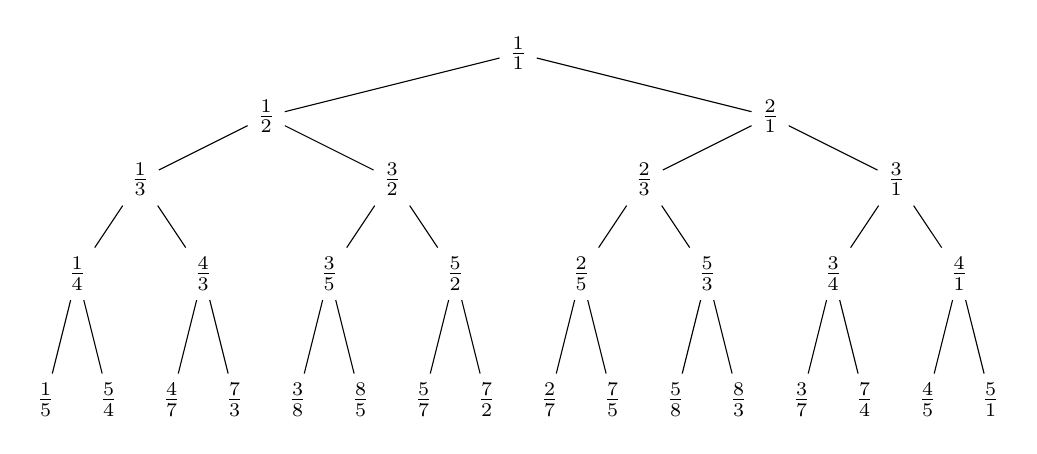
\begin{tikzpicture}[scale=0.8]
\path
(0,0)     node[] (1) {$\frac{1}{1}$}
+(-4,-1) node[] (2) {$\frac{1}{2}$}
+(4,-1)   node[] (3) {$\frac{2}{1}$}
(2)
+(-2,-1)  node[] (4) {$\frac{1}{3}$}
+(2,-1)   node[] (5) {$\frac{3}{2}$}
(3)
+(-2,-1)   node[] (6) {$\frac{2}{3}$}
+(2,-1)  node[] (7) {$\frac{3}{1}$}
(4)
+(-1,-1.5) node[] (8) {$\frac{1}{4}$}
+(1,-1.5)  node[] (9) {$\frac{4}{3}$}
(5)
+(-1,-1.5) node[] (10) {$\frac{3}{5}$}
+(1,-1.5)  node[] (11) {$\frac{5}{2}$}
(6)
+(-1,-1.5) node[] (12) {$\frac{2}{5}$}
+(1,-1.5)  node[] (13) {$\frac{5}{3}$}
(7)
+(-1,-1.5) node[] (14) {$\frac{3}{4}$}
+(1,-1.5)  node[] (15) {$\frac{4}{1}$}
(8)
+(-.5,-2) node[] (16) {$\frac{1}{5}$}
+(.5,-2)  node[] (17) {$\frac{5}{4}$}
(9)
+(-.5,-2) node[] (18) {$\frac{4}{7}$}
+(.5,-2)  node[] (19) {$\frac{7}{3}$}
(10)
+(-.5,-2) node[] (20) {$\frac{3}{8}$}
+(.5,-2)  node[] (21) {$\frac{8}{5}$}
(11)
+(-.5,-2) node[] (22) {$\frac{5}{7}$}
+(.5,-2)  node[] (23) {$\frac{7}{2}$}
(12)
+(-.5,-2) node[] (24) {$\frac{2}{7}$}
+(.5,-2)  node[] (25) {$\frac{7}{5}$}
(13)
+(-.5,-2) node[] (26) {$\frac{5}{8}$}
+(.5,-2)  node[] (27) {$\frac{8}{3}$}
(14)
+(-.5,-2) node[] (28) {$\frac{3}{7}$}
+(.5,-2)  node[] (29) {$\frac{7}{4}$}
(15)
+(-.5,-2) node[] (30) {$\frac{4}{5}$}
+(.5,-2)  node[] (31) {$\frac{5}{1}$}
;
\draw (2)--(1)--(3) (4)--(2)--(5) (6)--(3)--(7) (8)--(4)--(9) 
(10)--(5)--(11) (12)--(6)--(13) (14)--(7)--(15)
(16)--(8)--(17) (18)--(9)--(19) (20)--(10)--(21) (22)--(11)--(23)
(24)--(12)--(25) (26)--(13)--(27) (28)--(14)--(29) (30)--(15)--(31)
;
\end{tikzpicture}
\end{figure*}

从根节点$\dfrac{1}{1}$出发, 每个节点 $x$ 的左右两个子节点分别表示应用 $g(x)$ 和 $h(x)$. 表示成分数则是每个节点$\dfrac{i}{j}$的左右子节点分别是$\dfrac{i}{i+j}$和$\dfrac{i+j}{j}$. 从根节点出发, 按广度优先的顺序遍历这个树, 得到的序列为
\[\frac{1}{1}, \frac{1}{2},\frac{2}{1},\frac{1}{3},\frac{3}{2},\frac{2}{3},\frac{3}{1},\frac{1}{4},\frac{4}{3},\frac{3}{5},\frac{5}{2},\frac{2}{5},\frac{5}{3},\frac{3}{4},\frac{4}{1},\frac{1}{5},\frac{5}{4},\frac{4}{7},\frac{7}{3},\frac{3}{8},\frac{8}{5},\frac{5}{7},\frac{7}{2},\frac{2}{7},\frac{7}{5},\cdots\]
容易观察发现, 每个数的分子都是它前一个数的分母, 将每一项的分子拿出来, 组成数组 $b_n$, 则原来有理数每一项为 $a_n = \dfrac{b_n}{b_{n+1}}$, 而分子 $b_n$为:
\[1, 1, 2, 1, 3, 2, 3, 1, 4, 3, 5, 2, 5, 3, 4, 1, 5, 4, 7, \cdots\]
$b_n$表示正整数 $n$ 表示成 $2$ 的幂次之和的方法数, 且每个幂使用不超过两次. 例如,  $b_5 = 2$ 对应两种表示方法: $5=4+1=2+2+1$.

可以证明, $b_n$ 满足下面的递推关系: $b_{2n+1} = b_n, b_{2n+2} = b_n+b_{n+1}$. 考虑将 $2n+1$ 表示成 $2$ 的幂次之和, 因为 $2n+1$ 是奇数, 所以求和式中有且只有一个 $1$, 而求和式余下的 $2n$ 的分解方式与 $n$ 的分解方式是一一对应的, 因为将 $n$ 分解成 $2$ 的幂次之和, 然后每一项乘以 $2$, 就得到 $2n$ 的一种分解方法, 反之亦然. 对于 $2n+2$ 的分解, 可能有$0$ 或 $2$个 $1$, 分别对应将 $n+1$ 和 $n$ 的分解为 $2$ 的幂次之和的方法数.

一个节点$a_n = \dfrac{b_n}{b_{n+1}}$, 其左儿子为 $a_{2n+1} = \dfrac{b_{2n+1}}{b_{2n+2}} = \dfrac{b_n}{b_n+b_{n+1}}$, 右儿子为 $a_{2n+2} = \dfrac{b_{2n+2}}{b_{2n+3}} = \dfrac{b_n+b_{n+1}}{b_{n+1}}$. 只要满足$b_n$的递推关系, 树的节点与子节点的关系也是自动满足的.


\newpage
%------------------------------------------------------------------------------%
\section{Pick 定理}
平面直角坐标系中, 一个简单多边形的顶点全部都是整点(称为格点多边形), 用 $i$ 表示多边形内部的整点个数, $b$ 表示边界上的整点个数(包含顶点和边上的点), 则多边形的面积为
\[ A = i + \frac{b}{2} - 1.\]

\subsection{单位三角形}
首先证明: 若一个三角形的顶点都是整点, 并且边界和内部不含其他整点, 则这个三角形面积是 $\dfrac{1}{2}$.

不妨将三角形的一个顶点挪到原点 $O$, 设另外两个顶点的坐标分别为 $A = (x_1,y_1)$, $B = (x_2,y_2)$. 则 $\triangle OAB$ 的边界和内部不包含整点, 由对称性, $O,A,A+B,B$ 四个点围成的平行四边形的边界和内部也不包含整点. 以 $\vec{OA}, \vec{OB}$ 为基, 构建平行四边形网格, 则其中每个平行四边形边界和内部都不包含整点. 
考虑 $(1,0)$ 和 $(0,1)$, 他们只可能是某个平行四边形的顶点. 设
\begin{align*}
m_1\cdot \vec{OA} + m_2\cdot \vec{OB} &= (1,0) \\
m_3\cdot \vec{OA} + m_4\cdot \vec{OB} &= (0,1)
\end{align*}
这里 $m_1,m_2,m_3,m_4$ 都是整数. 写成矩阵形式
\[
\begin{bmatrix}
m_1 & m_2 \\
m_3 & m_4
\end{bmatrix} \cdot
\begin{bmatrix}
x_1 & y_1 \\
x_2 & y_2
\end{bmatrix} =
\begin{bmatrix}
1 & 0 \\
0 & 1
\end{bmatrix} 
\]

两边求行列式:
\[ \mathrm{det}\left(
\begin{bmatrix}
m_1 & m_2 \\
m_3 & m_4
\end{bmatrix}
\right)\cdot\mathrm{det}\left(
\begin{bmatrix}
x_1 & y_1 \\
x_2 & y_2
\end{bmatrix}
\right) = 1\]

因为 $m_1,m_2,m_3,m_4, x_1, x_2, y_1, y_2$ 都是整数, 所以上面两个行列式也都是整数. 于是两个行列式只能是 $\pm 1$, 则 $|x_1y_2-x_2y_1| = 1$. 它正好是 $\vec{OA},\vec{OB}$ 张成的平行四边形的面积. 所以 $\triangle OAB$ 的面积为 $\dfrac{1}{2}$.

\subsection{推广至多边形}
将格点多边形分割成一个个格点三角形, 使得每个格点三角形内部和边上不含整点, 于是这个三角剖分构成平面图, 可以套用欧拉公式. 

平面图的顶点数为 $V=i+b$, 为原多边形边界(包含顶点)和内部所有的整点. 

设原多边形面积为 $A$, 剖分之后每个三角形面积都是 $\dfrac{1}{2}$, 则总面数为 $F = 2A$ (这里除去了最外面的那个面). 

全体的边分为两部分: 一部分是原多边形边上的, 沿着多边形边界走一圈会经过 $b$ 个整点, 剖分后被分成了 $b$ 条边; 另一部分在多边形内部, 每条边与两个面邻接, 而每个面有三条边, 则 $3F = 2E - b$, 可得 $E = \dfrac{3F+b}{2}$.

最后, 用欧拉公式: $V-E+F=1$ (这里也除去了最外面的那个面), 有
\[i+b - \frac{6A+b}{2} + 2A = 1.\]
于是
\[ A = i + \frac{b}{2} - 1 .\]


\newpage
%------------------------------------------------------------------------------%
\section{福特圆与法里和}
\subsection{福特圆}

福特圆是欧氏平面上的一组圆, 对于任意一个最简分数 $\dfrac{p}{q}$, 都对应一个福特圆, 圆心在 $( \dfrac{p}{q}, \dfrac{1}{2q^2} )$, 半径为 $\dfrac{1}{2q^2}$, 因此福特圆总是与 $x$ 轴相切.
\begin{figure*}[htbp]
\centering
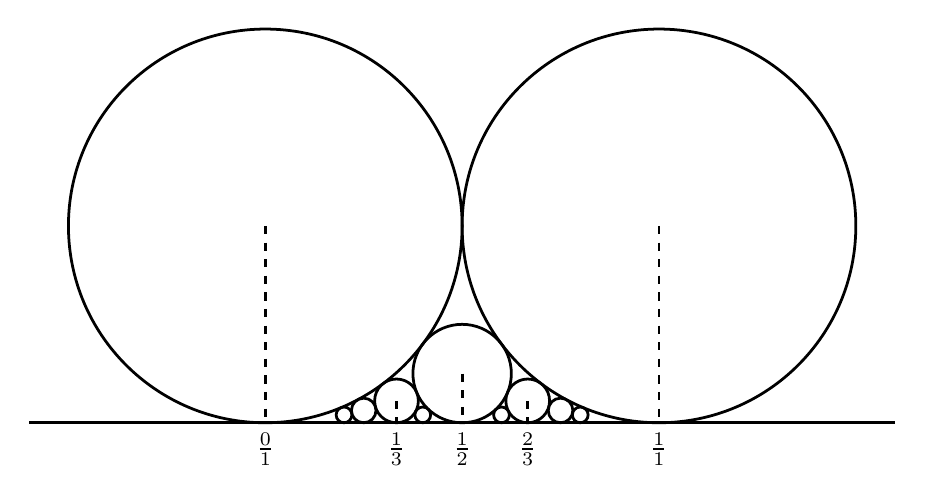
\begin{tikzpicture}[scale=5]
\coordinate[] (O) at (0,0);
\draw[line width=1pt] (-0.6,0)--(1.6,0) ;
\draw[line width=1pt] (0,0.5) circle (0.5);
\draw[line width=1pt] (1,0.5) circle (0.5);
\draw[line width=1pt] (0.5,0.125) circle (0.125);
%\draw[line width=1pt] (-0.5,0.125) circle (0.125);
\draw[line width=1pt] (0.3333,0.05555555) circle (0.05555555);
\draw[line width=1pt] (0.6666,0.05555555) circle (0.05555555);
%\draw[line width=1pt] (-0.3333,0.05555555) circle (0.05555555);
\draw[line width=1pt] (0.25,0.03125) circle (0.03125);
\draw[line width=1pt] (0.75,0.03125) circle (0.03125);
\draw[line width=1pt] (0.2,0.02) circle (0.02);
\draw[line width=1pt] (0.4,0.02) circle (0.02);
\draw[line width=1pt] (0.6,0.02) circle (0.02);
\draw[line width=1pt] (0.8,0.02) circle (0.02);
\draw[line width=1pt,dashed] (0,0.5) -- (0,0);
\draw[line width=1pt,dashed] (1,0.5) -- (1,0);
\draw[line width=1pt,dashed] (0.5,0.125) -- (0.5,0);
\draw[line width=1pt,dashed] (0.3333,0.05555555) -- (0.3333,0);
\draw[line width=1pt,dashed] (0.6666,0.05555555) -- (0.6666,0);
\node [anchor=north] at (0,0) {$\frac{0}{1}$};
\node [anchor=north] at (0.3333,0) {$\frac{1}{3}$};
\node [anchor=north] at (0.6666,0) {$\frac{2}{3}$};
\node [anchor=north] at (0.5,0) {$\frac{1}{2}$};
\node [anchor=north] at (1,0) {$\frac{1}{1}$};
%\foreach \p in {O,A,B}
%	\fill[fill=black,draw=black,thick] (\p) circle (0.2pt);
\end{tikzpicture}
\end{figure*}

福特圆有一个有趣的性质, 若两个最简分数 $\dfrac{p}{q}$ 和 $\dfrac{r}{s}$, 满足 $|ps-qr|=1$, 则它们对应的福特圆相切; 否则两个福特圆相离, 不会出现相交的情况.
下面是一个简单的证明.
\begin{figure*}[htbp]
\centering
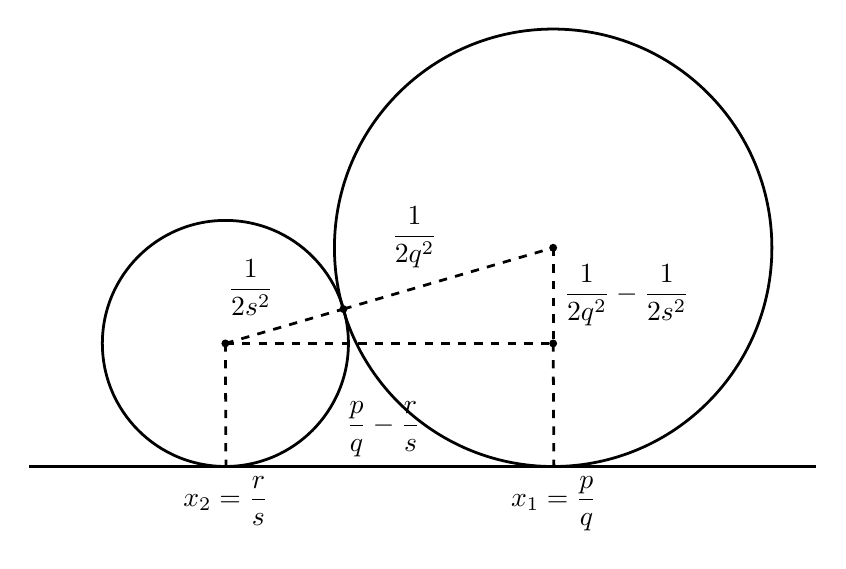
\begin{tikzpicture}[scale=50]
\coordinate[] (A) at (0.3333,0.05555555);
\coordinate[] (B) at (0.25,0.03125);
\coordinate[] (C) at (0.28,0.04);
\coordinate[] (D) at (0.3333,0.03125);
\draw[line width=1pt] (0.2,0)--(0.4,0) ;
\draw[line width=1pt] (A) circle (0.05555555);
\draw[line width=1pt] (B) circle (0.03125);

\draw[line width=1pt,dashed] (A) to[edge label=$\dfrac{1}{2q^2} - \dfrac{1}{2s^2}$] (D);
%\draw[decorate,decoration={brace,raise=2},line width=1pt] (A) -- (D);
\draw[line width=1pt,dashed] (D) -- (0.3333,0);
\draw[line width=1pt,dashed] (B) -- (0.25,0);
\draw[line width=1pt,dashed] (B) to[edge label=$\dfrac{1}{2s^2}$] (C);
\draw[line width=1pt,dashed] (C) to[edge label=$\dfrac{1}{2q^2}$] (A);
\draw[line width=1pt,dashed] (B) -- (D);
\node [anchor=north] at (0.3333,0) {$x_1=\dfrac{p}{q}$};
\node [anchor=north] at (0.25,0) {$x_2=\dfrac{r}{s}$};
\node [anchor=south] at (0.29,0) {$\dfrac{p}{q} - \dfrac{r}{s}$};
\foreach \p in {A,B,C,D}
	\fill[fill=black,draw=black,thick] (\p) circle (0.02pt);
\end{tikzpicture}
\end{figure*}

若两个福特圆相切, 需要满足下面的关系:
\begin{align*}
\left(\frac{p}{q} - \frac{r}{s}\right)^2 + \left( \frac{1}{2q^2} - \frac{1}{2s^2} \right)^2 &= \left( \frac{1}{2q^2} + \frac{1}{2s^2} \right)^2 \\
\frac{(ps-qr)^2}{q^2s^2} &= 4\cdot \frac{1}{2q^2}\cdot\frac{1}{2s^2}\\
(ps-qr)^2 &= 1
\end{align*}
即 $|ps-qr| = 1$. 
该过程反向也是成立的,  即只要 $|ps-qr| = 1$, 则对应的两个福特圆就相切. 
而如果 $|ps-qr| > 1$, 将得到
$$ \left(\frac{p}{q} - \frac{r}{s}\right)^2 + \left( \frac{1}{2q^2} - \frac{1}{2s^2} \right)^2 > \left( \frac{1}{2q^2} + \frac{1}{2s^2} \right)^2 ,$$
也就是两个福特圆相离. $|ps-qr| < 1$, 因为 $p,q,r,s$ 都是整数, 所以只能是 $|ps-qr| = 0$, 或写成 $\dfrac{p}{q} = \dfrac{r}{s}$. 但 $\dfrac{p}{q}$ 和 $\dfrac{r}{s}$ 都是最简分数, 则只能是 $p=r, q=s$, 也就是两圆重合.


\subsection{法里和}
福特圆还有另一个有趣的性质. 如果两个最简分数$\dfrac{p}{q},\dfrac{r}{s}$ 对应的福特圆相切, 则在这两圆之间还存在一个福特圆与它们分别相切, 其对应的最简分数为 $\dfrac{p+r}{q+s}$. 

不失一般性, 可以假设 $\dfrac{p}{q} < \dfrac{r}{s}$, 根据两圆相切的条件, 可知 $qr - ps = 1$. 并且容易证明 $\dfrac{p}{q} < \dfrac{p+r}{q+s} < \dfrac{r}{s}$, 事实上, 
\[\frac{p+r}{q+s} - \frac{p}{q} = \frac{pq+rq-pq-ps}{(q+s)q} = \frac{1}{(q+s)q} > 0 .\]
类似的有 $\dfrac{p+r}{q+s} - \dfrac{r}{s} < 0$. 所以 $\dfrac{p+r}{q+s}$ 位于 $\dfrac{p}{q}$ 和 $\dfrac{r}{s}$ 之间.

然后证明 $\dfrac{p+r}{q+s}$ 是最简分数. 从上面的计算过程可知
\[ q(p+r) - p(q+s) = 1 .\]
$p+r$与$q+s$的整数倍线性组合能得到$1$, 由裴蜀定理可得$p+r$与$q+s$互素.

再证明 $\dfrac{p+r}{q+s}$ 对应的福特圆与$\dfrac{p}{q},\dfrac{r}{s}$ 对应的福特圆分别相切. 根据相切条件, 只要满足:
\[ |(p+r)q - (q+s)p| = 1 ,\]
以及
\[ |(p+r)s - (q+s)r| = 1  .\]
而这两个条件在 $qr - ps = 1$ 时都是成立的.

像这样将两个最简分数的分子和分母分别相加的操作称为法里和, 或法里加法, 英文文献中记为 mediant 或 Farey Addition.
















\chapter{代数}

\section{不等式}

已知 $a,b,c,d$ 为正实数, 求证
\[22a + 25b + 30c + 30d \ge 360 \sqrt[3]{\frac{abcd}{2a+5b+10c+30d}},\]
并确定等式成立的条件.

证明: 

\begin{align*}
2a+5b+10c+30d &=10\cdot\frac{a}{5}+20\cdot\frac{b}{4}+30\cdot\frac{c}{3}+60\cdot\frac{d}{2} \\
& \ge 120\sqrt[120]{\left(\frac{a}{5}\right)^{10}\cdot\left(\frac{b}{4}\right)^{20}\cdot\left(\frac{c}{3}\right)^{30}\cdot\left(\frac{d}{2}\right)^{60}}\\
&= 120\sqrt[12]{\left(\frac{a}{5}\right)\cdot\left(\frac{b}{4}\right)^2\cdot\left(\frac{c}{3}\right)^3\cdot\left(\frac{d}{2}\right)^6}
\end{align*}

所以
\begin{align*}
\sqrt[3]{\frac{abcd}{2a+5b+10c+30d}} &\le \sqrt[3]{\frac{abcd}{120\sqrt[12]{(\frac{a}{5})\cdot(\frac{b}{4})^2\cdot(\frac{c}{3})^3\cdot(\frac{d}{2})^6}}} \\
&= \sqrt[36]{\frac{a^{11}\cdot b^{10}\cdot c^9\cdot d^6}{2^{26}\cdot 3^9\cdot 5^{11}}} \\
&= \sqrt[36]{\left(\frac{a}{5}\right)^{11}\cdot\left(\frac{b}{4}\right)^{10}\cdot\left(\frac{c}{3}\right)^{9}\cdot\left(\frac{d}{2}\right)^6}\\
\end{align*}

进而
\begin{align*}
22a+25b+30c+30d &= 10\cdot\left[11\cdot(\frac{a}{5})+10\cdot(\frac{b}{4})+9\cdot(\frac{c}{3})+6\cdot(\frac{d}{2})\right] \\
&\ge 10\cdot 36\sqrt[36]{\left(\frac{a}{5}\right)^{11}\cdot\left(\frac{b}{4}\right)^{10}\cdot\left(\frac{c}{3}\right)^{9}\cdot\left(\frac{d}{2}\right)^6}\\
&\ge 360 \sqrt[3]{\frac{abcd}{2a+5b+10c+30d}}
\end{align*}

等号在 $a:b:c:d=5:4:3:2$ 时取得.

~
\newpage
%------------------------------------------------------------------------------%

\noindent A.Oppenheim 不等式

设 $a,b,c,S$ 分别为 $\triangle ABC$ 的三边长和面积, 则对任意 $x,y,z\in R$ 有
\[(xa^2+yb^2+zc^2)^2 \ge 16S^2(xy+yz+zx) .\]
等号成立当且仅当 $a^2:b^2:c^2=(y+z):(z+x):(x+y)$.

\begin{wrapfigure}[4]{o}{0pt}
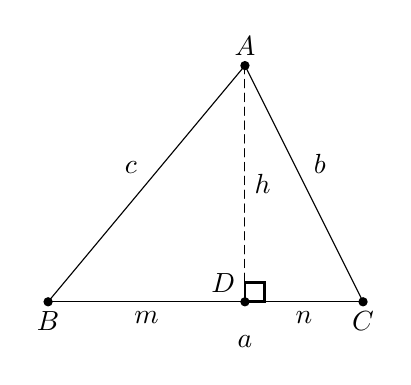
\begin{tikzpicture}[cap=round,scale=1]
\tikzstyle{axes}=[line width=1pt]
\coordinate[label=135:$D$,] (D) at (0.0,0.0);
\coordinate[label=below:$B$] (B) at (-2.5,0.0);
\coordinate[label=below:$C$] (C) at (1.5,0.0);
\coordinate[label=above:$A$] (A) at (0.0,3.0);
\draw[] (B) to [edge label = $c$] (A);
\draw[] (A) to [edge label = $b$] (C);
\draw[] (C) to [edge label = $n$] (D);
\draw[] (D) to [edge label = $m$] (B);
\draw[densely dashed] (A) to [edge label = $h$] (D);
\foreach \p in {A,B,C,D}
	\fill[fill=black,draw=black,thick] (\p) circle (1.25pt);
\draw[] (0,-0.5) node {$a$};
\tkzMarkRightAngle[line width=1pt](A,D,C);
\end{tikzpicture}
\end{wrapfigure}
~

\begin{proof}
如图, 过$A$点作$BC$边上的高 $AD=h$, 有
\begin{align*}
 k&=xa^2+yb^2+zc^2\\
&=x(m+n)^2+y(n^2+h^2)+z(m^2+h^2)\\
&=x(m+n)^2+(yn^2+zm^2)+(y+z)h^2\\
&\ge x(m+n)^2+\frac{(m+n)^2}{\frac{1}{y}+\frac{1}{z}}+(y+z)h^2\\
&= \frac{xy+yz+zx}{y+z}(m+n)^2+(y+z)h^2\\
&\ge 2\sqrt{xy+yz+zx}(m+n)h\\
&=4\sqrt{xy+yz+zx}\cdot S
\end{align*}

两个不等号分别使用了权方和不等式(或柯西不等式变形)及均值不等式.

于是, $S\le \dfrac{k}{4\sqrt{xy+yz+zx}}$, 等号成立当且仅当 $a^2:b^2:c^2=(y+z):(z+x):(x+y)$.
\end{proof}

~

\noindent 补充:

事实上, 第一个不等号只要用到权方和不等式的特殊形式即可: 
\begin{align*}
\left(\frac{1}{y}+\frac{1}{z}\right)(ym^2+zn^2) &= m^2 + n^2 + \frac{y}{z}m^2 + \frac{z}{y}n^2\\
&\ge m^2+n^2 + 2\sqrt{\frac{y}{z}m^2\cdot\frac{z}{y}n^2}\\
&=(m+n)^2
\end{align*}
于是有 
\[
(ym^2+zn^2) \ge \frac{(m+n)^2}{\frac{1}{y}+\frac{1}{z}}.
\]

\newpage
%------------------------------------------------------------------------------%
若 $\triangle ABC$ 的三边 $a,b,c$ 满足 $a^2+b^2+3c^2=7$, 求 $\triangle ABC$ 面积的最大值.

~

\noindent 解法一: 可以直接用 A.Oppenheim 不等式, 令$x=1,y=1,z=3$, 则
\[S\le\frac{xa^2+yb^2+zc^2}{4\sqrt{xy+yz+zx}} = \frac{\sqrt{7}}{4}. \]

~

\noindent 解法二: 由三角形面积公式, 以余弦定理:
\begin{align*}
S &= \frac{1}{2}ab\sin C \\
&= \frac{1}{2}ab\sqrt{1-\cos^2 C}\\
&= \frac{1}{2}ab\sqrt{1-\left(\frac{a^2+b^2-c^2}{2ab}\right)^2}\\
&= \frac{1}{2}\sqrt{(ab)^2-\frac{(a^2+b^2-c^2)^2}{4}}\\
&=\frac{1}{2}\sqrt{(ab)^2-\frac{(7-4c^2)^2}{4}}
\end{align*}
又因为 $ab\le\dfrac{a^2+b^2}{2}=\dfrac{7-3c^2}{2}$, 所以
\begin{align*}
S &=\frac{1}{2}\sqrt{(ab)^2-\frac{(7-4c^2)^2}{4}}\\
& \le\frac{1}{2}\sqrt{\frac{(7-3c^2)^2}{4}-\frac{(7-4c^2)^2}{4}}\\
&= \frac{1}{4}\sqrt{-7(c^2-1)^2+7}\\
&\le \frac{\sqrt{7}}{4}.
\end{align*}

~

\noindent 解法三: 设 $D$ 是 $AB$ 的中点, 由三角形中线长公式: $\displaystyle CD = \frac{1}{2}\sqrt{2(a^2+b^2)-c^2}$.

即 $4CD^2 + c^2 = 2(a^2+b^2)$, 而 $a^2+b^2+3c^2=7$, 所以
\[2CD^2+\frac{7}{2}c^2=a^2+b^2+3c^2=7.\]
等式左边根据均值不等式有: 
\[2CD^2+\frac{7}{2}c^2 \ge 2\sqrt{7}CD\cdot c\ge 2\sqrt{7}h_c\cdot c.\]
所以 $S=\dfrac{1}{2}h_c\cdot c \le \dfrac{1}{2}\cdot\dfrac{7}{2\sqrt{7}}=\dfrac{\sqrt{7}}{4}.$

\newpage
%------------------------------------------------------------------------------%
\section{函数}

\noindent 2019南京大学计算机拔尖班二次选拔:

假设$f$是定义在正整数集合上, 取值也总是正整数的一个函数, 并且满足对于任意的正整数 $m,n$, 若 $m-n$ 也是正整数, 那么 $f(m+n)f(m-n)=f(m^2)$, 求所有满足条件的函数 $f$.

~

解: 先取$n=1,2$, 有:
\[ f(m+1)f(m-1) = f(m^2) = f(m+2)f(m-2) .\]
于是得到: $\dfrac{f(m+2)}{f(m+1)} = \dfrac{f(m-1)}{f(m-2)}$. 

可以看出$\dfrac{f(m+2)}{f(m+1)}$ 的值是周期为 3 的序列. 按 $x$ 模3 的余数, 分别讨论$f(x)$:

(a) 若 $x=3k$, 则 $\dfrac{f(3k+2)}{f(3k+1)} = \dfrac{f(3k-1)}{f(3k-2)} = \cdots = \dfrac{f(5)}{f(4)} = \dfrac{f(2)}{f(1)}$, 所以
\[f(3k+2) = \dfrac{f(2)}{f(1)}f(3k+1) .\]

(b) 若 $x=3k+1$, 则 $\dfrac{f(3k+3)}{f(3k+2)} = \dfrac{f(3k)}{f(3k-1)} = \cdots = \dfrac{f(6)}{f(5)} = \dfrac{f(3)}{f(2)}$, 所以
\[f(3k+3) = \dfrac{f(3)}{f(2)}f(3k+2) .\]

(c) 若 $x=3k-1$, 则 $\dfrac{f(3k+1)}{f(3k)} = \dfrac{f(3k-2)}{f(3k-3)} = \cdots = \dfrac{f(7)}{f(6)} = \dfrac{f(4)}{f(3)}$, 注意到取 $m=2$, $n=1$时, 根据题目条件有$f(3)f(1)=f(4)$, 所以
\[f(3k+1) = \dfrac{f(4)}{f(3)}f(3k) = f(1)f(3k) .\]

综合 (a)(c) 有: $f(3k+2)=f(2)f(3k)$; 

综合 (a)(b)(c) 有: $f(3k+3) = f(3)f(3k)$. 这意味着 $f(3k)$ 是一个等比数列, 通项公式为 $f(3k)=f(3)^k$.

进一步有: $f(3k+2)=f(2)f(3)^k, f(3k+1) = f(1)f(3)^k$

回到原条件, 取 $m=3k$, $n=1$, 得 
\begin{align*}
f(3k+1)f(3k-1) &=f(9k^2) \\
f(1)f(3)^k \cdot f(2)f(3)^{k-1} &= f(3)^{3k^2}\\
f(1)f(2) &= f(3)^{3k^2-2k+1}
\end{align*} 
$f(1)f(2)$ 是定值, 说明 $f(3)^{3k^2-2k+1}$ 对任意的 $k$ 都是定值, 于是只有 $f(3)=1$. 

而 $f(1), f(2)$ 都是整数, 并且$f(1)f(2)=1$, 因此必有 $f(1)=f(2)=1$.

所以满足题目条件的函数只有 $f(x)=1$.


\newpage
%------------------------------------------------------------------------------%
\noindent 2022中科大少年班复试

记 $g(x)=x^2-k$, $h(x)=g(g(x))$, $k$ 为整数.

(1) 写出$h(x)$ 的表达式;

(2) 求集合 $A=\{ x\in \mathbb{R} | h(x) = x\}$;

(3) 已知函数 $f: A\rightarrow A$ 满足 $f(f(x)) = g(x)$, 证明: $f$ 既是单射也是满射;

(4) 是否存在函数 $s(x)$, 使得$s(s(x))=x^2-2$, 证明你的结论.

~

\noindent 解: 

(1)\ \ \ $h(x) = (x^2-k)^2-k$.

~

(2)\ \ \ 当 $g(x)=x$ 时, $h(x)=g(g(x))=x$, 意味着 $g(x)-x=0$ 的根也属于集合 $A$. 于是可以进行因式分解:
\[ h(x)-x =  (x^2-k)^2-k - x = (x^2-x-k)(x^2+x+1-k) \]
两项的判别式分别是 $\Delta_1 = 1+4k$, $\Delta_2 = 1-4(1-k)=4k-3$. 令
\[x_{1,2}=\frac{1\pm\sqrt{\Delta_1}}{2},\qquad x_{3,4}=\frac{-1\pm\sqrt{\Delta_2}}{2} ,\]
考虑到$k$是整数,
当 $k < -\dfrac{1}{4}$ 时, $A=\varnothing$;
当 $-\dfrac{1}{4} < k < \dfrac{3}{4}$ 时, $A=\{x_1, x_2\}$;
当 $k > \dfrac{3}{4}$ 时, $A=\{x_1, x_2, x_3, x_4\}$.

~

(3)\ \ \ 先证单射: 若 $a,b\in A$, 且满足 $f(a)=f(b)$, 则 $g(a)=f(f(a))=f(f(b))=g(b)$, 进一步有 $h(a)=g(g(a))=g(g(b))=h(b)$, 由 $a,b\in A$ 得 $h(a)=a$ 和 $h(b)=b$, 所以推出 $a=b$, 于是单射得证.

~

再证满射: 对任意 $a\in A$, 有 $a = h(a)=g(g(a))=f(f(f(f(a))))$, 只要取 $x = f(f(f(a)))$, 可知$x\in A$, 并且有 $f(x)=a$. 于是满射也得证.

(4)\ \ \ $g(x)=x^2-2$, $A$ 中存在 4 个元素, 分别为 $x_1 = -1$, $x_2=2$, $x_3=\dfrac{-1-\sqrt{5}}{2}$, $x_4=\dfrac{-1+\sqrt{5}}{2}$. 可以直接计算验证 $g(x_1)=x_1$, $g(x_2)=x_2$, $g(x_3)=x_4$, $g(x_4)=x_3$. 

根据第(3)问, 若存在 $s(x)$, 使得 $s(s(x))=g(x)$, 则 $s: A\rightarrow A$ 是一个双射函数. 看看$s$ 将 $x_3$ 映射到多少. 

假设$s(x_3)=x_3$, 则 $g(x_3)=s(s(x_3))=x_3$, 这与 $g(x_3)=x_4$ 矛盾.

假设$s(x_3)=x_4$, 那么因为 $s$ 是双射, 所以$s(x_4)\ne x_4$, 于是 $g(x_3)=s(s(x_3))=s(x_4)\ne x_4$, 同样与 $g(x_3)=x_4$ 矛盾.

假设$s(x_3)=x_1$, 则 $x_4 = g(x_3)=s(s(x_3))=s(x_1)$, 两边再用 $s$ 作用得: $s(x_4) = s(s(x_1)) = g(x_1)=x_1=s(x_3)$, 与$s$ 是双射矛盾. 

假设$s(x_3)=x_2$, 跟上一条类似.

所以不存在这样的 $s$.


\newpage
%------------------------------------------------------------------------------%
\noindent 半群一定存在幂等元:

设 $A$ 是有限集, 定义运算$\otimes$满足:

(1) 封闭性: 对任意 $x,y\in A$, 有 $x\otimes y\in A$;

(2) 结合律: 对任意 $x,y,z\in A$, 有 $(x\otimes y)\otimes z = x\otimes(y\otimes z)$.

证明: 存在$\alpha\in A$, 使得 $\alpha\otimes\alpha=\alpha$.


~

解: 固定 $x\in A$, 若 $x\otimes x = x$, 则已经找到幂等元, 否则, 可以构造序列 $\{a_n\}$, 其中 $a_1=x\otimes x$, $a_{n}=a_{n-1}\otimes a_{n-1}$. 因为 $\otimes$ 满足封闭性, 所以序列 $\{a_n\}$ 是 $A$ 的子集, 而 $A$  是有限集, 所以 $\{a_n\}$ 必然有重复元素, 于是可以设 $a_s = a_t, s<t$. 再取出之间的一段作为序列$\{b_m\}$, 即
\begin{align*}
b_1&=a_s,\\ 
b_2&=a_{s+1}=b_1\otimes b_1 = b_1^2,\\ 
b_3&=a_{s+2}=b_2\otimes b_2 = b_1^4,\\
&\cdots\\ 
b_m&=a_{t-1} = b_{m-1}\otimes b_{m-1} = b_1^{2^{m-1}},\\
b_1&=a_t=b_{m}\otimes b_m=b_1^{2^m}.
\end{align*}
上述等式从第二行往下, 左边有一个 $b_1, \cdots, b_m$, 右边有两个, 考虑将它们乘起来.
\[b_2\otimes b_3\otimes\cdots b_m\otimes b_1 = (b_1\otimes b_1)\otimes(b_2\otimes b_2)\otimes\cdots(b_m\otimes b_m).\]
用$b_1$ 表示 $b_2,\cdots,b_m$, 再根据结合律, 可以发现其实 $\{b_1, \cdots, b_m\}$ 之间的运算是满足交换律的. 上式左边等于 $b_1^{2+4+\cdots+2^{m-1}+1}$, 右边等于 $b_1^{2+4+\cdots+2^m}$, 于是只要令 $y=b_2\otimes b_3\otimes\cdots b_m\otimes b_1$, 就有 $y=y\otimes y$, 也就构造出了幂等元.

~

解法2: 固定 $x\in A$, 由于 $A$ 是有限集且具有封闭性, 所以存在 $s,t\in\mathbb{N}$, 使得 $x^s = x^{s+t}$, 从而对任意正整数 $k$, 当 $k\ge s$ 时, 都有 $x^k=x^{k+t}$. 这样, 当 $k\ge s$ 时, $x^k=x^{k+t}=x^{k+2t}=\cdots=x^{k+mt}$ 对任意 $m$ 都成立.

取$k$是$t$ 的倍数$k=qt$, $q\in\mathbb{N}^+$, 并且$q$足够大, 满足 $k\ge s$, 于是
\[ (x^k)^2 = x^{qt}\otimes x^k=x^{qt+k}=x^k .\]
这样, $\alpha=x^k$ 满足 $\alpha^2=\alpha$.

\newpage
%------------------------------------------------------------------------------%
\noindent $\sqrt{2}$ 是无理数的一种奇特证法

因为 $1<\sqrt{2}<2$, 有 $0<\sqrt{2}-1<2$. 考虑序列 $s_n = (\sqrt{2}-1)^n$, 它总是具有 $A_n\sqrt{2}+B_n$ 的形式. 这里 $A_n, B_n$ 都是整数.

倘若 $\sqrt{2}$ 是有理数, 设 $\sqrt{2} = p/q$, 其中 $p,q$ 是正整数. 则 $A_n\sqrt{2}+B_n$ 的分母是 $q$, 且 $s_n>0$, 从而 $s_n \ge 1/q$. 但是 $s_n$ 是趋于 0 的, 矛盾.

\newpage
%------------------------------------------------------------------------------%

\noindent 堆垒求和方法
\[ S(n,k) = \sum_{i=1}^{n}{i^k} \]

首先, $ k = 1 $ 时, \[ S(n,1) = 1 + 2 + \cdots + n = \frac{(n+1)n}{2} .\]

当 $ k = 2 $ 时, 因为
\begin{align*}
(n+1)^3 &= n^3 + 3n^2 + 3n + 1 \\ 
n^3 &= (n-1)^3 + 3(n-1)^2 + 3(n-1) + 1\\
\cdots & \\
 2^3 &= 1^3 + 3\cdot 1^2 + 3\cdot 1 + 1
\end{align*}

两边全部加起来, 得到: 
\begin{align*} 
(n+1)^3 &= 1 + 3\cdot(1^2+2^2+\cdots+n^2) + 3\cdot(1+2+\cdots+n) + n \\
	&= 1 + 3S(n,2) + 3S(n,1) + n\\
3S(n,2) &= (n+1)^3 - 3S(n,1) - n - 1 \\
	S(n,2) &= \frac{n(n+1)(2n+1)}{6} .
\end{align*}

当 $ k = 3 $ 时, 有:
\begin{align*} 
(n+1)^4 &= n^4 + 4n^3 + 6n^2 + 4n + 1 \\
		&= 1 + 4S(n,3) + 6S(n,2) + 4S(n,1) + n
\end{align*} 

也可以同理推出来.

\newpage
%------------------------------------------------------------------------------%
求和: 
$\displaystyle \sum_{n=1}^{\infty}{\frac{n^3}{2^n}}$ .

\noindent 反复利用堆垒求和即可. 令 $S_k$ = $\displaystyle \sum_{n=1}^{\infty}{\frac{n^k}{2^n}}$, 则:
\begin{align*}
S_0 &= \sum_{n=1}^{\infty}{\frac{1}{2^n}} = 1 \\
S_1 &= \sum_{n=1}^{\infty}{\frac{n}{2^n}} \\
2S_1 &= \sum_{n=1}^{\infty}{\frac{n}{2^{n-1}}} = 1+\sum_{n=1}^{\infty}{\frac{n+1}{2^{n}}} \\
&= 1+\sum_{n=1}^{\infty}{\frac{n}{2^{n}}} + \sum_{n=1}^{\infty}{\frac{1}{2^{n}}} = 1 + S_1 + S_0\\
S_1 &= 2 \\
S_2 &= \sum_{n=1}^{\infty}{\frac{n^2}{2^n}} \\
2S_2 &= \sum_{n=1}^{\infty}{\frac{n^2}{2^{n-1}}} = 1 + \sum_{n=1}^{\infty}{\frac{(n+1)^2}{2^n}}\\ 
&= 1 + \sum_{n=1}^{\infty}{\frac{n^2}{2^n}} + \sum_{n=1}^{\infty}{\frac{2n}{2^n}} + \sum_{n=1}^{\infty}{\frac{1}{2^n}} = 1 + S_2 + 2S_1 + S_0 \\
S_2 &= 6 \\
S_3 &= \sum_{n=1}^{\infty}{\frac{n^3}{2^n}} \\
2S_3 &=   \sum_{n=1}^{\infty}{\frac{n^3}{2^{n-1}}} = 1 + \sum_{n=1}^{\infty}{\frac{(n+1)^3}{2^n}} \\
&= 1 +  \sum_{n=1}^{\infty}{\frac{n^3}{2^n}} +  \sum_{n=1}^{\infty}{\frac{3n^2}{2^n}} +  \sum_{n=1}^{\infty}{\frac{3n}{2^n}} +  \sum_{n=1}^{\infty}{\frac{1}{2^n}} \\
&= 1 + S_3 + 3S_2 + 3S_1 + S_0\\
S_3 &= 26
\end{align*}

~

\noindent 也可以用生成函数的方法. 令 
\[f(x) =  \sum_{n=1}^{\infty}{\frac{x^n}{2^n}} = \frac{x}{2-x} ,\]
则对 $f(x)$ 求导, 并继续构造, 依次可以得到:
\begin{align*}
f'(x) &=  \sum_{n=1}^{\infty}{\frac{n\cdot x^{n-1}}{2^n}} = \left( \frac{x}{2-x} \right)' = \frac{2}{(2-x)^2} \\
g(x) &= x\cdot f'(x) = \sum_{n=1}^{\infty}{\frac{n\cdot x^n}{2^n}} = \frac{2x}{(2-x)^2} \\
g'(x) &= \sum_{n=1}^{\infty}{\frac{n^2 \cdot x^{n-1}}{2^n}} = \frac{4+2x}{(2-x)^3} \\
h(x) &= x\cdot g'(x) = \sum_{n=1}^{\infty}{\frac{n^2\cdot x^n}{2^n}} = \frac{4x+2x^2}{(2-x)^3} \\
h'(x) &= \sum_{n=1}^{\infty}{\frac{n^3\cdot x^{n-1}}{2^n}} = \frac{(4+4x)(2-x)+3(4x+2x^2)}{(2-x)^4}
\end{align*}

令 $x=1$, 代入 $h'(x)$, 得到
\[h'(1) = \sum_{n=1}^{\infty}{\frac{n^3}{2^n}} = 26 .\]

\newpage
%------------------------------------------------------------------------------%

\noindent 生成函数, 多项式系数, 以及集合计数

\noindent 问题: 集合 $\{1,2,\cdots ,2000\}$ 的所有子集中, 元素之和能被 5 整除的子集有多少个. (来自 102 Combinatorial Problems From the Training of the USA IMO Team)

~

\noindent 解: 考虑多项式 
\begin{align*}
f(x) &= (1+x)(1+x^2)(1+x^3)\cdots(1+x^{2000}) \\
&= c_0 + c_1x + c_2x^2 + \cdots .
\end{align*}
它的展开式中 $x^n$ 的系数 $c_n$ 对应了和为 $n$ 的子集个数. 因为对于子集 $\{a_1, a_2, \cdots, a_m\}$ 和展开式中的项 $x^{a_1}x^{a_2}\cdots x^{a_m}$ 存在一一映射. 所以我们要寻找形如 $x^{5k}$ 项的系数之和.

可以取不同的 $x$, 并求和, 依次来消掉一些项, 例如, $f(1)+(f-1) = 2(c_0+c_2+c_4+\cdots)$, 就消去了奇数项, 从而可以求出偶数项系数之和.

类似地, 令 $ \xi = e^{2\pi i/5}$ 为 5 次单位根, 即 $\xi^5 = 1$, 易知 $1+\xi+\xi^2+\xi^3+\xi^4=0$. 而当$x = \xi, \xi^2, \xi^3, \xi^4$ 时, 集合 $\{x, x^2, x^3, x^4\} = \{\xi, \xi^2, \xi^3, \xi^4\}$. 所以
\begin{align*}
\sum_{n=0}^4{f(\xi^n)} &= 5c_0 + c_1(1+\xi+\xi^2+\xi^3+\xi^4)+c_2(1+\xi+\xi^2+\xi^3+\xi^4) + \cdots \\
&= 5(c_0+c_5+c_{10} + \cdots ).
\end{align*}
这样就只留下了 5 的倍数次幂的系数.

那么 $\displaystyle \sum_{n=0}^4{f(\xi^n)}$ 究竟是多少呢? 因为 $\xi^n$ 的幂次的值以 5 为周期, 即$\xi^{(m+5k)n}=\xi^{mn}$, 所以$f(\xi^n)$只是 5 个不同的数重复乘了 400 次, 即 
\[f(\xi^n)=\left[(1+\xi^n)(1+\xi^{2n})\cdots(1+\xi^{5n})\right]^{400}\]
当 $n=1,2,3,4$ 时,
\[f(\xi^n) = \left[(1+\xi)(1+\xi^{2})\cdots(1+1)\right]^{400}.\]
当 $n=0$ 时, $f(\xi^n)=2^{2000}$.

又因为 $\xi, \xi^2, \cdots, \xi^5$ 是 $g(x)=x^5-1$ 的 5 个根, 所以有如下的因式分解:
\[g(x) = x^5-1=(x-\xi)(x-\xi^2)(x-\xi^3)(x-\xi^4)(x-\xi^5).\]
将 $x=-1$ 代入 $g(x)$ 得 $-2 = -2(1+\xi)(1+\xi^2)(1+\xi^3)(1+\xi^4)$, 于是所有 5 次项的系数之和为
\[\frac{1}{5}\sum_{n=0}^4{f(\xi^n)}=\frac{1}{5}\left(4\times 2^{400}+2^{2000}\right) = \frac{1}{5}\left(2^{402}+2^{2000}\right).\]


\newpage
%------------------------------------------------------------------------------%
求正整数 $ x $,$ y $ 和素数 $ p $,满足 $ x^3+y^3=p^2 $。

解:由 
\begin{equation*}
p^2=x^3+y^3=(x+y)(x^2-xy+y^2 )
\end{equation*}

知 $ p=x+y=x^2-xy+y^2 $,或写成 $ x^2-(y+1)x+(y^2-y)=0 $。

对 $ x $ 用求根公式,则
\[ 
x=\frac{(y+1)\pm\sqrt{(y+1)^2-4(y^2-y)}}{2} 
\]

根号内满足:$ (y+1)^2-4(y^2-y)=6y-3y^2+1\ge 0 $,所以 $ y $ 只可能取 1 或 2。

$ y=1 $ 时,$ x=2 $;$ y=2 $ 时,$ x=1 $;这两个解都满足。

\newpage
%------------------------------------------------------------------------------%
问题: $ [a] $ 表示不大于 $ a $ 的最大整数。自然数 $ n $ 满足:$ n=[n/2]+[n/3]+\cdots +[n/2010] $,求所有符合条件的 $ n $。

解:首先 $ n $ 一定小于 2010。所以 $ n=[n/2]+[n/3]+\cdots +[n/n] $。

可是又有 $ [n/2],[n/3],\cdots [n/n] $ 都至少为 1,而右边有 $ n-1 $ 项,所以有 $ [n/2]=2 $,其他项都等于 1,于是 $ n=4 $ 或 5。

~

问题: 证明对任何 $x\ge 3$, $x$ 进制数 $(2221)_x$ 在十进制下永远不会是 3 的倍数.

解: $(2221)_x = 2x^3+2x^2+2x+1 = 2(x-1)x(x+1)+2(x+1)^2-1$, 当 $x$ 模 3 等于 $0,1,2$ 时, 该多项式都不能被 3 整除. 所以得证.


%------------------------------------------------------------------------------%
\newpage
对于每个自然数 $ n $,定义 $ f(n)=m $,而 $ m $ 满足:

(1). 存在一个递增的自然数序列 $ a_1<a_2<\cdots <a_k $,其中 $ a_1 = n, a_k=m $,使得这个序列的乘积 $ a_1a_2\cdots a_k $ 是完全平方数。注意 $ m $ 总是存在的,因为 $ n = a_1 < a_2 = 4n $ 时,$ a_1a_2=4n^2 $ 就能满足这个条件。

(2). $ m $ 是令上面条件成立的最小的数。例如 $ f(1) = 1, f(2) = 6, f(3) = 8, f(4) = 4 $,等等。

求证:$ f(n) $ 是自然数到 $ \{1\} \cup \{\text{合数} \} $ 的一一对应。

~

解:首先证明 $ f(n) $ 一定不是素数。这是显然的,因为如果存在一个素数 $ p $ 满足条件1的话,考虑乘积 $ a_1a_2\cdots p $,它的 $ p $ 的幂次是1,从而不可能是完全平方数,矛盾。

然后证明 $ f(n) $ 是单射。即 $ f(a) = f(b) $ 时必有 $ a = b $。这里用反证法。如果 $ a \neq b $ 且 $ f(a) = f(b) $,不失一般性,假设 $ a < b $,则存在下面两个序列:
\begin{align*}
a = a_1 < a_2 < \cdots < a_s = f(a) \\
b = b_1 < b_2 < \cdots < b_t = f(b)
\end{align*}
令集合 $ A = \{a_1, a_2, \cdots, a_s\}, B = \{b_1, b_2, \cdots, b_t\} $,令集合 $ C = A\cup B - A\cap B $,其中的元素为 $ c_1 < c_2 < \cdots < c_r $。因为 $ a,b $ 都属于 $ C $,而 $ a < b $,可知 $ a $ 是 $ C $ 中最小的元素。又因为 $ f(a) \in A\cap B $,所以 $ f(a) \notin C $,从而有 $ c_r < f(a) $。

注意到乘积 
\[
a_1a_2\cdots a_sb_1b_2\cdots b_t,
\]
它是一个完全平方数,并且集合 $ A\cap B $ 中的每个元素在其中出现过两次,所以把它们都除去以后,剩下的乘积就是 $ c_1c_2\cdots c_r $,它仍然是完全平方数。这样一来对于自然数 $ a $ 就找到一个递增的序列 $ c_1 < c_2 < \cdots < c_r $,满足条件(1),且 $ c_r < f(a) $,这与条件(2)矛盾。所以 $ f(n) $ 是单射。

再证明 $ f(n) $ 是满射。这里可以尝试从 $ f $ 的逆映射入手,对于一个合数 $ m $,定义映射 $ F(m)=n $ 满足:

(1'). 存在一个递增的序列 $ b_1 < b_2 < \cdots < b_k $,其中 $ b_1 = n, b_k = m $,使乘积 $ b_1b_2\cdots b_k $ 为完全平方数。这里 $ n $ 总是找得到的,因为把 $ m $ 没有配对的素因子找出来:$ m=p_1p_2\cdots p_j q^2 $,其中 $ p_1<p_2<\cdots<p_j $ 是互不相同的素数。则 $ p_1p_2\cdots p_jm $ 就是完全平方数,$ n $ 取 $ p_1 $即可。

(2'). $ n $ 是满足上面条件最大的自然数。

如果 $ n = F(m) $,则 $ f(n) \le m $。用反证法。假设 $ f(n) < m $,这里 $ f $ 和 $ F $ 各有一个序列:
\begin{align*}
n&=a_1<a_2<\cdots < a_s = f(n) < m \\ 
n&=b_1<b_2<\cdots < b_t = m
\end{align*}

集合 $ A = \{a_1,\cdots,a_s\}, B = \{b_1,\cdots,b_t\}$,又令集合 $ C = A\cup B - A\cap B $,其中的元素为 $ c_1 < c_2 < \cdots < c_r $。$ m\in B $ 且 $ m\notin A $,所以 $ m \in C $,而 $ m $ 又是 $ A,B $ 两个集合中最大的元素,所以 $ m = c_r$。类似前面的推理可知乘积 $ c_1c_2\cdots c_r $ 是完全平方数。而 $ n \notin C $,说明 $ c_1 > n $,这与定义 $ F $ 的条件(2')矛盾。于是必定有 $ f(n) = m $。

所以给定一个合数 $ m $,可以用 $ F $ 找到它在映射 $ f $ 下的原象,也就证明了 $ f $ 是满射。

\newpage

%------------------------------------------------------------------------------%
2016北京大学自主招生考试:

(单选)已知正整数 $ a,b,c,d $,满足 $ ab=cd $,则 $ a+b+c+d $ 有可能等于()?

A. 101 \hspace{4em}  B. 301 \hspace{4em}  C. 401 \hspace{4em}  D. 以上都不对

解:$ d $ 一定可以写成两个数 $ e,f $ 的乘积,满足 $ a $ 被 $ e $ 整除,$ b $ 被 $ f $ 整除。

考虑 $ (\dfrac{a}{e}+f)(\dfrac{b}{f}+e) = \dfrac{ab}{ef} + a + b + ef = a+b+c+d $,因为 $ (\dfrac{a}{e}+f) $ 和 $ (\dfrac{b}{f}+e) $ 都大于 1,而选项中只有一个合数 $ 301=7\times 43 $,简单取 $ e=f=1 $,那么有 $ a=6, b=42 $,满足条件。

\newpage

%------------------------------------------------------------------------------%
2019清华大学自主招生考试:

(填空)若正实数 $ a,b $ 满足 $ ab(a+8b) = 20 $,则 $ a + 3b $ 的最小值为\underline{\hspace{2em}}。

解:设 $ a = xb $,则 $ x(x+8)b^3=20 $,只要求下面式子的最小值即可:
\[ (a+3b)^3 = (x+3)^3b^3 = \frac{(x+3)^3}{x(x+8)} .\]
设 
\[ f(x) = \log \frac{(x+3)^3}{x(x+8)} = 3\log (x+3) - \log(x) - \log(x+8) \]
令它的导数等于0:
\[ f'(x) = \frac{3}{x+3}-\frac{1}{x}- \frac{1}{x+8} = 0\]
它的正实数根为 $ x = 2 $,所以所求最小值是 5.

\newpage

%------------------------------------------------------------------------------%

\noindent 1994 年土耳其数学奥林匹克: 

求满足 $ t^2+1=s(s+1) $ 的所有正整数对 $ (s,t) $.

解: 因为 $ s(s+1) $ 一定是偶数, 所以 $ t $ 一定是奇数. 令 $ t = 2k + 1 $, 其中 $ k \ge 0 $, 又设 $ s = 2k + x $, 其中 $ x $ 是整数. 

进一步, 如果 $ x \le 0 $, 则 $ s(s+1) < 4k^2+4k < t^2 + 1 $, 条件不满足. 于是 $ x > 0 $.

将 $ s $ 和 $ t $ 代入原条件可得 $ 4k^2 + 4k + 2 = 4k^2 + 4kx + x^2 + 2k + x $, 整理得到 
\[ 4k(x-1)+x^2+2k+x-2=0. \] 

因为 $ x $ 是大于 0 的整数, 且 $ k $ 是非负整数, 所以等式左边是分别关于 $ x $ 和 $ k $ 递增的. 当 $ x = 1, k = 0 $ 时有最小值 0.

所以本题的唯一解为: $ s = 1, t = 1 $.

\newpage

%------------------------------------------------------------------------------%

求下面方程组的所有实数解:
\[
\begin{cases}
1 - x^2 & = y \\
1 - y^2 & = z \\
1 - z^2 & = x 
\end{cases}
\]

解: 可以发现 $x,y,z $是对称的, 如果其中两个数相等, 不妨设 $ x=y $, 则有 $ y = 1 - x^2 = 1 - y^2 = z $, 说明只要任意两个数相等, 那么三个数都相等. 此时只要求 $ x^2 - x - 1 = 0 $, 得 $ x = y = z = \dfrac{1\pm \sqrt{5}}{2} $.

如果它们两两都不相等, 不失一般性, 可以设 $ x < y < z $. 则 $ 1-z^2 < 1-x^2 < 1-y^2 $, 或写成 $ z^2 > x^2 > y^2 $. 于是 $z$ 绝对值最大, $x$ 绝对值最小, 可以推断 $ x < 0 $, $ z > 0 $. 由 $ z = 1 - y^2 $ 可知 $ z \le 1 $, 于是 $ 0 < z \le 1 $, $ x = 1 - z^2 > 0 $, 导致了矛盾. 所以不可能出现三个数都不相等的情况.

\newpage
%------------------------------------------------------------------------------%
\noindent 来自每日数学打卡

已知复数 $a,b,c,x,y,z$ 满足:
\begin{align*}
& a = \frac{b+c}{x-2}, \qquad b = \frac{c+a}{y-2},\qquad c = \frac{a+b}{z-2},\\
& xy+yz+zx = 2021,\qquad x+y+z=2022.
\end{align*}
求 $xyz$ 的值.

~

解: 由条件可得
\begin{align*}
a &= \frac{b+c}{x-2}\\
x-2 &= \frac{b+c}{a}\\
x-1 &= \frac{a+b+c}{a}\\
\frac{1}{x-1} &= \frac{a}{a+b+c}.
\end{align*}
同理可得, $\dfrac{1}{y-1} = \dfrac{b}{a+b+c}, \dfrac{1}{z-1} = \dfrac{c}{a+b+c}$.
所以, 
\[\frac{1}{x-1} + \frac{1}{y-1}+\frac{1}{z-1} = 1.\]
通分可得
\[\frac{(y-1)(z-1)+(x-1)(z-1)+(x-1)(y-1)}{(x-1)(y-1)(z-1)} = 1.\]
展开:
\[ (xy + yz + zx) - 2(x+y+z) + 3 = xyz - (xy+yz+zx) + (x+y+z) - 1.\]
所以
\[xyz = 2(xy+yz+zx) - 3(x+y+z) + 4 = -2020.\]


\newpage
%------------------------------------------------------------------------------%

第 5 届 IMO 试题

求证:
\[
 \cos(\frac{\pi}{7})-\cos(\frac{2\pi}{7})+\cos(\frac{3\pi}{7})=\frac{1}{2}.
\]
\begin{wrapfigure}{o}{5cm}
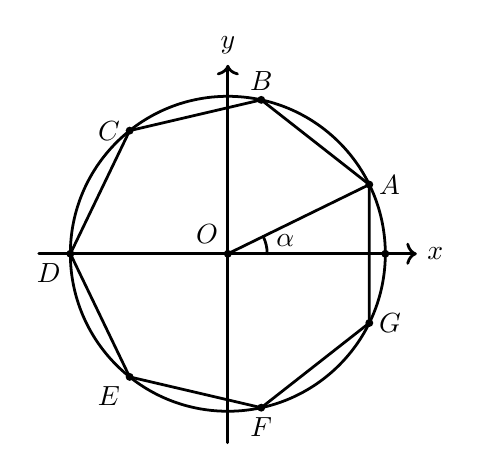
\begin{tikzpicture}[cap=round,scale=2.0]
\tikzstyle{axes}=[line width=1pt]
\coordinate[label=right:$A$] (A) at (0.8982934325496409,0.43939607308006734);
\coordinate[label=right:$G$] (G) at (0.8982934325496409,-0.43939607308006734);
\coordinate[label=above:$B$] (B) at (0.21206921921340208,0.9772546476032836);
\coordinate[label=below:$F$] (F) at (0.21206921921340208,-0.9772546476032836);
\coordinate[label=left:$C$] (C) at (-0.6234898077068194,0.7818314778043369);
\coordinate[label=below left :$E$] (E) at (-0.6234898077068194,-0.7818314778043369);
\coordinate[label=below left:$D$] (D) at (-1,0);
\coordinate (X) at (1,0);
\coordinate[label=above left:$O$] (O) at (0,0);
\draw [line width=1pt] (O) circle (1cm);
\draw [line width=1pt] (O)-- (A);
\draw [line width=1pt] (A) --(B)--(C)--(D)--(E)--(F)--(G)--(A);
\begin{scope}[style=axes]
    \draw[->] (-1.2,0) -- (1.2,0) node[right] {$x$};
    \draw[->] (0,-1.2) -- (0,1.2) node[above] {$y$};
\end{scope}
\foreach \p in {A,B,C,D,E,F,G,O,X}
	\fill[fill=black,draw=black,thick] (\p) circle (0.5pt);
\draw pic["$\alpha$",draw,line width=1pt, angle eccentricity=1.5, angle radius=0.5cm] {angle=X--O--A};

\end{tikzpicture}
\end{wrapfigure}
\indent 解:如图所示,$ \angle \alpha $ 的值为 $ \dfrac{\pi}{7} $,$ ABCDEFG $ 对应的辐角为 $ \alpha $ 的奇数倍。

$ A $ 和 $ G $ 的 $ x $ 坐标为 $ \cos(\dfrac{\pi}{7}) $,$ B $ 和 $ F $ 的 $ x $ 坐标为 $ \cos(\dfrac{3\pi}{7}) $,$ C $ 和 $ E $ 的 $ x $ 坐标为 $ \cos(\dfrac{5\pi}{7}) $,或 $ -\cos(\dfrac{2\pi}{7}) $.\\
\indent 这 7 个点分别与原点构成的相交加起来为 0 向量,或者:
\[
2\cos(\frac{\pi}{7})+2\cos(\frac{3\pi}{7})-2\cos(\frac{2\pi}{7})-1=0.
\]
结论得证。

~

~

\newpage
%------------------------------------------------------------------------------%

\noindent 环球城市数学竞赛~ 1980 春季~ 初中组/高中组

边长为 1 的正方形内部有有限条线段, 
每条线段平行于正方形某一条边, 线段总长度为 18. 
这些线段和原来正方形的四条边一起将正方形分成了若干个两两不相交的区域.

求证: 这些小区域中至少有一个的面积不小于 0.01.

~

证明: 假设这些小区域的周长为 $ p_i $, 面积为 $ S_i $, 因为正方形内部的每条线段贡献了两个小区域的周长, 而正方形的边贡献了一个小区域的周长, 所以这些小区域的周长之和为 
\[ \sum_i{p_i} = 18\times 2 + 4 = 40 .\]

令第 $ i $ 个区域的 AABB (axis aligned bounding box) 长宽为 $ a_i, b_i $, 则有:
\[ p_i \ge 2(a_i+b_i),\quad s_i \le a_i b_i .\]
所以
\[ \sum_i{\sqrt{s_i}} \le \sum_i{\sqrt{a_i b_i}} \le \frac{1}{2}\sum_i{(a_i+b_i)} \le \frac{1}{4}\sum_i{p_i} = 10 .\]

如果对于对于所有的 $ s_i $都小于 0.01, 则 $ \sqrt{s_i} < 0.1 $, 
\[ \sum_i{s_i} = \sum_i{(\sqrt{s_i}\cdot\sqrt{s_i})} < \sum_i{0.1\sqrt{s_i}} < 0.1\sum_i{\sqrt{s_i}} \le 1 .\]
这与 $ \sum_i{\sqrt{s_i}} = 1 $ 矛盾.

所以一定存在一个 $ s_i $ 不小于 0.01.

\newpage

%------------------------------------------------------------------------------%

\noindent 环球城市数学竞赛~ 1980 春季~ 高中组

空间中有 30 个向量, 求证一定存在两个向量夹角小于 $ 45 \degree $.

\begin{figure}[htbp]
\centering

\begin{minipage}[t]{0.49\linewidth}
\centering
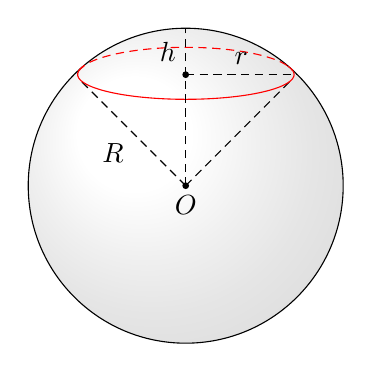
\begin{tikzpicture}[]
  \coordinate (O) at (0,0);
\coordinate (1) at (0,1.41);
\coordinate (2) at (0,2);
\coordinate (3) at (1.41,1.41);
  % ball background color
  \shade[ball color = white, opacity = 0.2] (0,0) circle [radius = 2cm];
  % ball
  \draw (O) circle [radius=2cm];
  % label of ball center point
  \filldraw (O) circle (1pt) node[below] {$O$};
  % radius
  \draw[densely dashed] (O) to [edge label = $R$] (-1.33,1.33);
  \draw[densely dashed] (O) -- (1.33,1.33);
  % cut of ball surface
  %\draw[red] (-1.35,1.47) arc [start angle = 140, end angle = 40, x radius = 17.6mm, y radius = 14.75mm];	% top
  \draw[red, densely dashed] (-1.36,1.46) arc [start angle = 170, end angle = 10, x radius = 13.8mm, y radius = 3.6mm];
  \draw[red] (-1.29,1.52) arc [start angle=-200, end angle = 20, x radius = 13.75mm, y radius = 3.15mm];
\filldraw (1) circle (1pt);
\draw (0.0,1.7) node[left] {$h$};
\draw[densely dashed] (1) to [edge label = $r$] (3);
\draw[densely dashed] (O) -- (2);
  % label of cut of ball surface
  %\draw (-1.2,2.2) -- (-0.53,1.83) node at (-1.37,2.37) {$A$};
\end{tikzpicture}
\end{minipage}
\begin{minipage}[t]{0.49\linewidth}
\centering
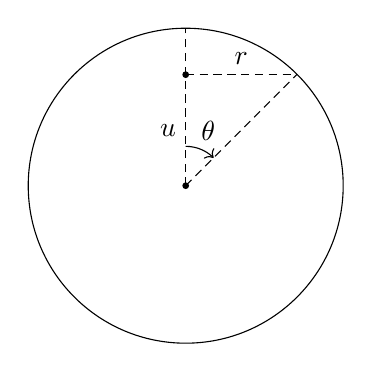
\begin{tikzpicture}[]
  \coordinate (O) at (0,0);
\coordinate (1) at (0,1.41);
\coordinate (2) at (0,2);
\coordinate (3) at (1.41,1.41);
  \draw (O) circle [radius=2cm];
  % label of ball center point
  \filldraw (O) circle (1pt);
  \draw[densely dashed] (O) to (3);
  \filldraw (1) circle (1pt);
\draw (0.0,0.7) node[left] {$u$};
\draw[densely dashed] (1) to [edge label = $r$] (3);
\draw[densely dashed] (O) -- (2);
\draw (0,2) coordinate (a) (0,0) coordinate (b) (1.41,1.41) coordinate (c) pic["$\theta$", draw,<-, angle eccentricity=1.5, angle radius=0.5cm]{angle=c--b--a};
\end{tikzpicture}
\end{minipage}
\end{figure} 

先求球冠的面积公式, 假设球半径为 $ R $, 球冠高度为 $ h $, 则取球冠上的一圈, 半径为 $ r = R\sin\theta $, 一圈长度为 $ 2\pi r = 2\pi R\sin\theta$, 宽度为 $ R \text{d}\theta $, 面积微元是 $ 2\pi R^2\sin\theta\text{d}\theta $. 
令 $ u = R\cos\theta $, 则 $ \text{d}u = -R\sin\theta\text{d}\theta $. 当 $ \theta $ 从 0 增加时, $ u $ 的变化范围是 $ R $ 到 $ R-h $. 面积为
\[ \int_{0}^\Theta {2\pi R^2\sin\theta\text{d}\theta} = \int_{R}^{R-h}{-2\pi R\text{d}u} = 2\pi Rh .\]

将这些向量起点挪到原点, 每个向量对应一个张角 $ 45 \degree $ (单侧张角 $ 22.5 \degree $) 的圆锥. 每个圆锥在单位球上截出一个球冠, 如果有两个球冠相交, 说明对应的两个向量夹角小于 $ 45 \degree $.

二倍角公式: $ \cos 2x = 2 \cos^2 x - 1 $, 得半角公式 $ \cos x = \sqrt{ \dfrac{\cos 2x+1}{2} } $

球冠高度为 \[ h = 1 - \cos 22.5\degree = 1 - \frac{\sqrt{2+\sqrt{2}}}{2} .\]

30 个球冠的面积为 \[ 30\times 2\pi Rh = 60\pi \left( 1 - \frac{\sqrt{2+\sqrt{2}}}{2} \right).\]

球的表面积为 $ 4\pi $. 比较发现 30 个球冠面积更大, 说明一定有球冠相交.

\newpage

%------------------------------------------------------------------------------%

\noindent 环球城市数学竞赛~ 1982 春季~ 初中组

集合 $ S $ 定义为: \[ S = \left\{ \frac{1}{k} \mid k = 1, 2, \cdots \right\} .\] 问是否存在由 $ S $ 中的不同元素构成的等差数列, 如果有, 可能有多少项.

~

解: 对于任意的正整数 $ n $, 可以构造数列 \[ \left\{ \frac{1}{n!}, \frac{2}{n!}, \cdots, \frac{n}{n!} \right\}. \]
则它是等差数列, 且都是 $ S $ 中的元素. 可见能构造任意长度的等差数列.

\newpage

%------------------------------------------------------------------------------%
\section{组合计数}

问题:圆周上有 $ n $ 个点,将它们两两相连得到一些弦,假设任意三条弦都不会相交于同一点,求这些弦之间一共有多少交点。

解:每个交点对应了两条弦,或者 4 个顶点,考虑圆周上任意 4 个点,它们之间可以有且只有一种情况能产生两条弦在圆内相交的情况。也就是说,一个 4 个点的组合与圆内弦的交点是一一对应的,所以交点共有 $ C_n^4 $ 个。

\vbox{}

问题:圆周上有 $ n $ 个点,将它们两两相连得到一些弦,假设任意三条弦都不会相交于同一点,求这些弦把圆分成多少个区域。

解:初始时有一个区域,每增加一条弦,会多出一个区域,现在考虑弦之间的交点。假如圆内已经有了一些弦,再画一条弦,可能会与其中的一些产生交点。画的过程中,从新弦的一个端点出发,如果没有产生新的交点,那么同样只会多出一个区域,而每产生一个交点,会额外分出一个区域。所以区域的总数为 $ 1 + C_n^2 + C_n^4 $,后面两项分别是弦的个数和交点的个数。

注: 当$n=1,2,3,4,5$时, 结果分别是$1, 2, 4, 8, 16$, 但当$n=6$时, 结果是$31$.


\newpage

%------------------------------------------------------------------------------%

问题:$ n $ 是给定的正整数,求有多少种正整数的组合 $ (i,j,k,h) $,满足:
\[ 1\le i < j \le k < h \le n+1 .\]

解:直接解法考虑 $ j=k $ 和 $ j\neq k $ 两种情况,分别相当于从 $ n+1  $ 个数中选 3 个和 4 个数,方法数为 $ C_{n+1}^3 + C_{n+1}^4 = C_{n+2}^4 $.

另一种思路:问题等价于求有多少个正整数的组合 $ (i,j,k',h') $ 满足:
\[ 1\le i < j < k' < h' \le n+2 .\]
直接得到答案。


\vbox{}

问题:罐子中有 $ n $ 个黑球和 $ n $ 个白球,每次从罐子里拿出一个球,直到取完,取球过程中,至少出现一次取出的白球多于取出的黑球的取法有多少种。

解:考虑罐子里有 $ n + 1 $ 个白球和 $ n - 1 $ 个黑球的取球序列,总会出现取出的白球个数多于黑球的情况,第一次出现时,取出的球中白球比黑球多 1 个,剩下的球中也是白球比黑球多 1 个。现在将剩下的球黑白颠倒,对应了原问题的所求情况。所以取法共有 $ C_{2n}^{n-1} $ 种。

\vbox{}

问题:由数字 0 和 1 组成的序列中,如果相邻两位的数不一样称为一次翻转,一个长度为 $ m $ 的序列恰好有 $ n $ 次翻转的情况有多少种。

解:直接法,长度为 $ m $ 的序列有 $ m - 1 $ 个间隙,每个间隙都可以翻转,确定了 $ n $ 次翻转的位置,第一位是 0 或 1 分别对应了一个序列,所以情况有 $ 2 C_{m-1}^n $ 种。

\vbox{}

问题:由数字 0 和 1 组成的长度为 $ m $ 的序列中,一个 0 紧跟在一个 1 后面的这样一个二元组出现了 $ n $ 次,求有多少种情况。

解:出现一个 01 后,下次再要遇到一个 01 之前,需要经历一次从 1 到 0 的翻转。因为 01 出现了 $ n $ 次,序列第一位和最后一位的数字与 1 到 0 的翻转出现的次数如下:

第一位是 0,最后一位也是 0,10 出现 $ n $ 次;

第一位是 0,最后一位是 1,10 出现 $ n - 1 $ 次;

第一位是 1,最后一位是 0,10 出现 $ n + 1 $ 次;

第一位是 1,最后一位也是 1,10 出现 $ n $ 次;

\noindent 所有情况加起来是 $ C_{m-1}^{2n} + C_{m-1}^{2n-1} + C_{m-1}^{2n+1} + C_{m-1}^{2n} = C_m^{2n} + C_m^{2n+1} = C_{m+1}^{2n+1} $.

另一个思路是考虑在原来序列前面补一个 1,后面补一个 0,这样原序列出现 $ n $ 次 01 等价于新序列发生 $ 2n+1 $ 次翻转(其中 0 到 1 发生 $ n $ 次,1 到 0 发生 $ n + 1 $ 次),而间隙有 $ m + 1 $ 个,所以可能的情况有 $ C_{m+1}^{2n+1} $ 种。

\vbox{}

问题:$ m $ 个白球和 $ n $ 个黑球排成一列,黑球不相邻的情况有多少种。

解:白球之间加上两端共有 $ m + 1$ 个空隙,选 $ n $ 个插入黑球,方法数为 $ C_{m+1}^n $.

另一个思路:除最后一个黑球外,其他黑球都吃掉它后面的一个白球,这样一共还剩 $ m + 1 $ 个球,将它们任意排列,之后除最后一个黑球之外的黑球再吐出一个白球,这就对应了一种黑球不相邻的序列。

\vbox{}

问题:圆周上有 $ m $ 个白球,编号为 $ 1,2,\cdots,m $,选出 $ n $ 个染黑,要求黑球不相邻,求方法数。

解:从 1 号断开,分两种情况。

(1) 1 号是白球,剩下的球中有 $ m - 1 - n $ 个白球和 $ n $ 个黑球,根据上一题结论,方法数为 $ C_{m-n}^n $;

(2) 1 号是黑球,从而 2 号和 $ m $ 号是白球,剩下的球中有 $ m - n - 2 $ 个白球和 $ n - 1 $ 个黑球,方法数为 $ C_{m-n-1}^{n-1} $.

加起来即可:
\begin{align*}
C_{m-n}^n + C_{m-n-1}^{n-1} &= 2C_{m-n}^n - C_{m-n-1}^n \\
& = \frac{2(m-n)!}{n!(m-2n)!} - \frac{(m-n-1)!}{n!(m-2n-1)!} \\
& = \frac{(m-n)!}{n!(m-2n)!}(2-\frac{m-2n}{m-n}) \\ 
& = \frac{m}{m-n} C_{m-n}^n
\end{align*}

\vbox{}

问题:三角形每条边被分成了 $ n $ 等分,连接这些分点,求图中有多少平行四边形。
\begin{figure*}[htbp]
\definecolor{sexdts}{rgb}{0.1803921568627451,0.49019607843137253,0.19607843137254902}
\definecolor{dtsfsf}{rgb}{0.8274509803921568,0.1843137254901961,0.1843137254901961}
\definecolor{rvwvcq}{rgb}{0.08235294117647059,0.396078431372549,0.7529411764705882}
\centering
\begin{minipage}[t]{0.49\linewidth}
\begin{tikzpicture}[line cap=round,line join=round,>=triangle 45,x=1cm,y=1cm,scale=0.8]
\clip(-4.5,-0.4) rectangle (4.95,5.15);
\draw [line width=1pt] (-4,0)-- (-2,4);
\draw [line width=1pt] (-2,4)-- (4,0);
\draw [line width=1pt] (4,0)-- (-4,0);
\draw [line width=1pt] (-2.25,3.5)-- (-1.25,3.5);
\draw [line width=1pt] (-2.5,3)-- (-0.5,3);
\draw [line width=1pt] (-2.75,2.5)-- (0.25,2.5);
\draw [line width=1pt] (1,2)-- (-3,2);
\draw [line width=1pt] (-3.25,1.5)-- (1.75,1.5);
\draw [line width=1pt] (2.5,1)-- (-3.5,1);
\draw [line width=1pt] (-3.75,0.5)-- (3.25,0.5);
\draw [line width=1pt] (-3,0)-- (-1.25,3.5);
\draw [line width=1pt] (-0.5,3)-- (-2,0);
\draw [line width=1pt] (-1,0)-- (0.25,2.5);
\draw [line width=1pt] (1,2)-- (0,0);
\draw [line width=1pt] (1,0)-- (1.75,1.5);
\draw [line width=1pt] (2.5,1)-- (2,0);
\draw [line width=1pt] (3,0)-- (3.25,0.5);
\draw [line width=1pt] (3,0)-- (-2.25,3.5);
\draw [line width=1pt] (-2.5,3)-- (2,0);
\draw [line width=1pt] (1,0)-- (-2.75,2.5);
\draw [line width=1pt] (-3,2)-- (0,0);
\draw [line width=1pt] (-1,0)-- (-3.25,1.5);
\draw [line width=1pt] (-3.5,1)-- (-2,0);
\draw [line width=1pt] (-3,0)-- (-3.75,0.5);
\begin{scriptsize}
\draw [fill=rvwvcq] (-4,0) circle (1.5pt);
\draw[color=rvwvcq] (-4.2,-0.2) node {$A$};
\draw [fill=rvwvcq] (4,0) circle (1.5pt);
\draw[color=rvwvcq] (4.2,-0.2) node {$B$};
\draw [fill=rvwvcq] (-2,4) circle (1.5pt);
\draw[color=rvwvcq] (-1.9171333333333305,4.229688888888887) node {$C$};
\end{scriptsize}
\end{tikzpicture}
\end{minipage}
\begin{minipage}[t]{0.49\linewidth}
\begin{tikzpicture}[line cap=round,line join=round,>=triangle 45,x=1cm,y=1cm,scale=0.8]
\clip(-4.5,-0.4) rectangle (4.95,5.15);
\draw [line width=1pt] (-4,0)-- (-2,4);
\draw [line width=1pt] (-2,4)-- (4,0);
\draw [line width=1pt] (4,0)-- (-4,0);
\draw [line width=1pt] (-2.25,3.5)-- (-1.25,3.5);
\draw [line width=1pt] (-2.5,3)-- (-0.5,3);
\draw [line width=1pt] (-2.75,2.5)-- (0.25,2.5);
\draw [line width=1pt] (1,2)-- (-3,2);
\draw [line width=1pt] (-3.25,1.5)-- (1.75,1.5);
\draw [line width=1pt] (2.5,1)-- (-3.5,1);
\draw [line width=1pt] (-3.75,0.5)-- (3.25,0.5);
\draw [line width=1pt,color=dtsfsf] (-3,0)-- (-1.25,3.5);
\draw [line width=1pt,color=dtsfsf] (-0.5,3)-- (-2,0);
\draw [line width=1pt] (-1,0)-- (0.25,2.5);
\draw [line width=1pt] (1,2)-- (0,0);
\draw [line width=1pt] (1,0)-- (1.75,1.5);
\draw [line width=1pt] (2.5,1)-- (2,0);
\draw [line width=1pt] (3,0)-- (3.25,0.5);
\draw [line width=1pt,color=sexdts] (3,0)-- (-2.25,3.5);
\draw [line width=1pt] (-2.5,3)-- (2,0);
\draw [line width=1pt,color=sexdts] (1,0)-- (-2.75,2.5);
\draw [line width=1pt] (-3,2)-- (0,0);
\draw [line width=1pt] (-1,0)-- (-3.25,1.5);
\draw [line width=1pt] (-3.5,1)-- (-2,0);
\draw [line width=1pt] (-3,0)-- (-3.75,0.5);

\begin{scriptsize}
\draw (-3.0,-0.25) node {$i$};
\draw (-2.0,-0.25) node {$j$};
\draw (1.0,-0.25) node {$k$};
\draw (3.0,-0.25) node {$h$};

\draw [fill=rvwvcq] (-4,0) circle (1.5pt);
\draw[color=rvwvcq] (-4.2,-0.2) node {$A$};
\draw [fill=rvwvcq] (4,0) circle (1.5pt);
\draw[color=rvwvcq] (4.2,-0.2) node {$B$};
\draw [fill=rvwvcq] (-2,4) circle (1.5pt);
\draw[color=rvwvcq] (-1.9171333333333305,4.229688888888887) node {$C$};
\end{scriptsize}
\end{tikzpicture}
\end{minipage}
\end{figure*}

解:这些平行四边形有 3 类,每一类的两组对边分别与原三角形的两条边平行,先考虑其中一类平行四边形,它的边分别与 $ AC $ 和 $ BC $ 平行。

延长与 $ AC $ 平行的边,与 $ AB $ 交于 $ i,j $ 两个分点,再延长与 $ BC $ 平行的边,与 $ AB $ 交于 $ k,h $ 两个分点。设 $ A,B $ 两点分别是线段 $ AB $ 的第 1 和第 $ n + 1 $ 个分点,则构成平行四边形的充要条件是 $ 1 \le i < j \le k < h \le n+1 $.

所以总个数为 $ 3C_{n+2}^4 $.

\vbox{}

问题: $m$ 个球放进 $n$ 个不同的罐子, 每个罐子至少有一个球, 有多少种可能性?

解: $m$ 个球排成一列, 相邻两球中间有一个空隙, 相当于要在这 $m-1$ 个空隙种选出 $n-1$ 个放入隔板, 隔板将一列球分成了 $n$ 段, 每个罐子里放入对应的段. 总共有 $C_{m-1}^{n-1}$ 种情况.


\vbox{}

问题: $m$ 个球放进 $n$ 个不同的罐子, 可以有空罐子, 有多少种可能性?

解: 再加入 $n$ 个球, 变成共 $m+n$ 个球放入 $n$ 个罐子, 每个罐子至少一个球的问题. 情况数是 $C_{m+n-1}^{n-1}$.

\newpage

%------------------------------------------------------------------------------%

可重复计数的证明:

从 $ [1,m] $ 范围取 $ n $ 个数,取出的数可以重复,总的取法有 $ C_{m+n-1}^n $ 种。 

例如:投 5 个骰子,一共会出现 $ C_{10}^{5} $ 种情况。

\begin{proof}

将取出来的数从小到大排列,设为 $ 1 \le a_1 \le a_2 \le \cdots \le a_n \le m $,等价于从 $ [1,m-n+1] $ 范围取 $ n $ 个数,满足 $ a_1 < a_2 < \cdots < a_n $,所以取法有 $ C_{m+n-1}^n $ 种。

\end{proof}

另一种思路:考虑 $ m - 1 $ 个白球和 $ n $ 个黑球排成一列,将第 $ i $ 个黑球之前的白球数量加 1 视为原问题中取出的第 $ i $ 大的数,答案就是 $ C_{m+n-1}^n $.

注意到第二种思路可以用来计算整数拆分的方法数。

\newpage

%------------------------------------------------------------------------------%

有一个宝箱,上面锁了一些锁,这些锁的钥匙被 $ n $ 个人保管,每个人有相同数量的钥匙,每个钥匙能开其中的一把锁。任意 $ k $ 个人将钥匙凑在一起可以打开全部的锁,而任意 $ k - 1 $ 个人的钥匙都不能打开全部锁。求至少需要多少把锁,以及此时每个人有多少把钥匙,以及此时任选 $ i $ 个人的组合中每个人都有的钥匙有多少种。

思路:考虑一个特定的人 $ A $,剩下 $ n - 1 $ 个人中任选 $ k - 1 $ 个人都会缺钥匙,而 $ A $ 正好有他们缺的钥匙。

注意到任意两个 $ k - 1 $ 人组合都不会缺同一把钥匙,如若不然,则这两个组合的并集至少有 $ k $ 个人,但他们还是缺一把钥匙,矛盾。

这就说明了 $ A $ 至少拥有剩下 $ n - 1 $ 个人中任选 $ k - 1 $ 个人的组合个数那么多把钥匙,也就是 $ C_{n-1}^{k-1} $。其他人的情况也一样,这样每个人都至少有这么多把钥匙。

另一方面,对于特定的一把锁,任意选 $ k $ 个人都能找到开它的钥匙,这就说明这个锁有 $ n - k + 1 $ 把钥匙。

综上所述,钥匙种类数量为 
\begin{align*} 
\frac{n}{n-k+1}C_{n-1}^{k-1} &= \frac{n}{n-k+1}\frac{(n-1)!}{(k-1)!(n-k)!} \\
				&=\frac{n!}{(k-1)!(n-k+1)!} \\
				&=C_n^{k-1}
\end{align*}

再考虑 $ n $ 个人取 $ k - 1 $ 个人的组合,这些组合都至少缺一个锁的钥匙,且没有两个组合会缺同一个锁的钥匙,所以锁至少有 $ C_n^{k-1} $ 个。














\chapter{几何}

\noindent 中线长公式:

$\triangle ABC$中, $BC$ 的中点为 $D$, 则 $AB^2 + AC^2 = 2(AD^2+BD^2)$.

\begin{figure*}[htbp]
\centering
\begin{tikzpicture}[cap=round,scale=1]
\tikzstyle{axes}=[line width=1pt]
\coordinate[label=below:$D$,] (D) at (0.0,0.0);
\coordinate[label=below:$B$] (B) at (-2.5,0.0);
\coordinate[label=below:$C$] (C) at (2.5,0.0);
\coordinate[label=above:$A$] (A) at (1.0,3.0);
\draw[] (B) to [edge label = $c$] (A);
\draw[] (A) to [edge label = $b$] (C);
\draw[] (C) to (B);
\draw[densely dashed] (A) to (D);
\foreach \p in {A,B,C,D}
	\fill[fill=black,draw=black,thick] (\p) circle (1.25pt);
\end{tikzpicture}
\end{figure*}

\begin{proof}
由余弦定理:
\begin{align*}
AB^2 &= AD^2+BD^2-2AD\cdot BD \cdot \cos\angle ADB, \\
AC^2 &= AD^2+CD^2-2AD\cdot CD \cdot \cos\angle ADC.
\end{align*}
又因为 $BD=CD$, 以及 $\cos\angle ADB=-\cos\angle ADC$, 所以上面两式相加得到:
\[AB^2 + AC^2 = 2(AD^2+BD^2).\]
\end{proof}


%------------------------------------------------------------------------------%
\newpage
托勒密定理: 圆内接四边形两条对角线的乘积等于两对对边乘积之和.

如下图所示, $ABCD$ 为圆内接四边形, 则对角线 $AC$ 与 $BD $ 的乘积等于一对对边 $AB$ 与 $CD$ 的乘积加上另一对对边 $AD$ 与 $BC$ 的乘积, 即 $AC\cdot BD = AB\cdot CD + AD\cdot BC$.

\begin{figure*}[htbp]
\centering
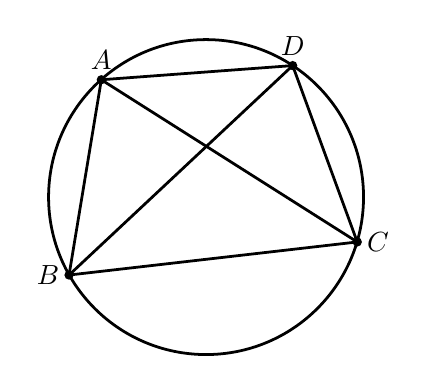
\begin{tikzpicture}[scale=1.0]
\coordinate[] (O) at (0,0);
\coordinate[label=left:$B$] (B) at (-1.74,-0.99);
\coordinate[label=$A$] (A) at (-1.33,1.49);
\coordinate[label=$D$] (D) at (1.1,1.67);
\coordinate[label=right:$C$] (C) at (1.92,-0.57);
\draw [line width=1pt] (O) circle (2cm);
\draw [line width=1pt] (A) -- (B) -- (C) -- (D) -- cycle;
\draw [line width=1pt] (A) -- (C);
\draw [line width=1pt] (B) -- (D);
\foreach \p in {A,B,C,D}
	\fill[fill=black,draw=black,thick] (\p) circle (1.25pt);
\end{tikzpicture}
\end{figure*}

证法1: (构造等角)

不失一般性, 可以假设 $\angle ADB < \angle BDC$, 过点 $D$ 作直线 $DE$ 交 $AC$ 于 $E$, 且满足 $\angle CDE = \angle ADB$, 如下图所示.
\begin{figure*}[htbp]
\centering
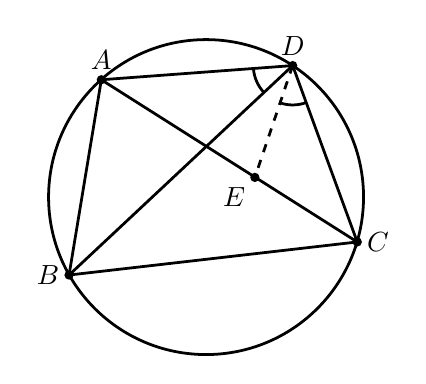
\begin{tikzpicture}[scale=1.0]
\coordinate[] (O) at (0,0);
\coordinate[label=left:$B$] (B) at (-1.74,-0.99);
\coordinate[label=$A$] (A) at (-1.33,1.49);
\coordinate[label=$D$] (D) at (1.1,1.67);
\coordinate[label=right:$C$] (C) at (1.92,-0.57);
\coordinate[label=below left:$E$] (E) at (0.62,0.25);
\draw [line width=1pt] (O) circle (2cm);
\draw [line width=1pt] (B) -- (A) -- (D) -- (C) -- cycle;
\draw [line width=1pt] (A) -- (C);
\draw [line width=1pt] (B) -- (D);
\draw [dashed,line width=1pt] (D) -- (E);
\foreach \p in {A,B,C,D,E}
	\fill[fill=black,draw=black,thick] (\p) circle (1.25pt);
\draw pic[draw,line width=1pt, angle eccentricity=1.5, angle radius=0.5cm] {angle=A--D--B};
\draw pic[draw,line width=1pt, angle eccentricity=1.5, angle radius=0.5cm] {angle=E--D--C};
\end{tikzpicture}
\end{figure*}

先证 $\triangle BDA \sim \triangle CDE$. 可以根据 $\angle BDA = \angle CDE$ 和 $\angle ABD = \angle ECD$ 得到. 于是 $AB : CE = BD : CD$, 即 $AB\cdot CD = BD\cdot CE$.

再证 $\triangle DBC \sim \triangle DAE$. 可以根据 $\angle DBC = \angle DAE$ 和 $\angle BDC = \angle ADE$ 得到. 于是 $BD : AD = BC : AE$, 即 $BD\cdot AE = BC\cdot AD$.

两式相加得: $BD\cdot(AE+CE) = AB\cdot CD + AD\cdot BC$, 即 $AC\cdot BD = AB\cdot CD + AD\cdot BC$.

~

证法2: (构造等角)
\begin{figure*}[htbp]
\centering
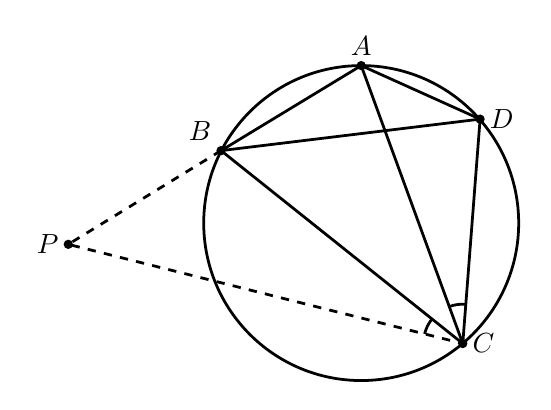
\begin{tikzpicture}[scale=1.0]
\coordinate[] (O) at (0,0);
\coordinate[label=$A$] (A) at (0,2);
\coordinate[label=above left:$B$] (B) at (-1.78,0.92);
\coordinate[label=right:$C$] (C) at (1.29,-1.53);
\coordinate[label=right:$D$] (D) at (1.51,1.32);
\coordinate[label=left:$P$] (P) at (-3.72,-0.27);
\draw [line width=1pt] (O) circle (2cm);
\draw [line width=1pt] (B) -- (A) -- (D) -- (C) -- cycle;
\draw [line width=1pt] (A) -- (C);
\draw [line width=1pt] (B) -- (D);
\draw [dashed,line width=1pt] (B) -- (P) -- (C);
\foreach \p in {A,B,C,D,P}
	\fill[fill=black,draw=black,thick] (\p) circle (1.25pt);
\draw pic[draw,line width=1pt, angle eccentricity=1.5, angle radius=0.5cm] {angle=D--C--A};
\draw pic[draw,line width=1pt, angle eccentricity=1.5, angle radius=0.5cm] {angle=B--C--P};
\end{tikzpicture}
\end{figure*}

在 $AB$ 的延长线上取一点 $P$, 使得 $\angle BCP = \angle DCA$, 于是 $\angle ACP = \angle DCB$.

再由 $\angle PAC = \angle BDC$, 得 $\triangle ACP\sim\triangle DCB$, 于是$AC:CD = AP:BD$, 即$AC\cdot BD = AP\cdot CD$.

另一方面, 根据 $\angle CBP=180\degree - \angle CBA = \angle CDA$ 和 $\angle BCP=\angle DCA$, 得 $\triangle ACD\sim\triangle PCB$, 于是 $AD:PB=CD:CB$, 即 $AD\cdot CB = CD\cdot BP$.

两式相减得到 $AC\cdot BD - AD \cdot CB = CD(AP-PB)$, 即 $AB\cdot CD+AD\cdot BC = AC\cdot BD$.

~

证法3: (正弦定理)
\begin{figure*}[htbp]
\centering
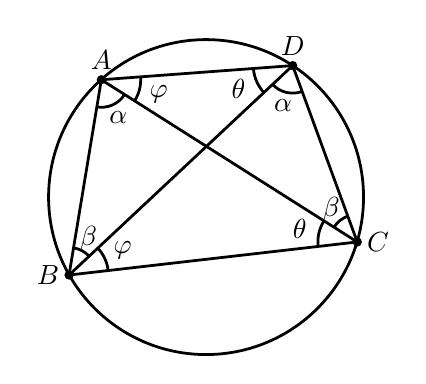
\begin{tikzpicture}[scale=1.0]
\coordinate[] (O) at (0,0);
\coordinate[label=left:$B$] (B) at (-1.74,-0.99);
\coordinate[label=$A$] (A) at (-1.33,1.49);
\coordinate[label=$D$] (D) at (1.1,1.67);
\coordinate[label=right:$C$] (C) at (1.92,-0.57);
\draw [line width=1pt] (O) circle (2cm);
\draw [line width=1pt] (B) -- (A) -- (D) -- (C) -- cycle;
\draw [line width=1pt] (A) -- (C);
\draw [line width=1pt] (B) -- (D);
\foreach \p in {A,B,C,D}
	\fill[fill=black,draw=black,thick] (\p) circle (1.25pt);
\draw pic["$\alpha$",draw,line width=1pt, angle eccentricity=1.5, angle radius=0.35cm] {angle=B--A--C};
\draw pic["$\alpha$",draw,line width=1pt, angle eccentricity=1.5, angle radius=0.35cm] {angle=B--D--C};
\draw pic["$\beta$",draw,line width=1pt, angle eccentricity=1.5, angle radius=0.35cm] {angle=D--B--A};
\draw pic["$\beta$",draw,line width=1pt, angle eccentricity=1.5, angle radius=0.35cm] {angle=D--C--A};
\draw pic["$\theta$",draw,line width=1pt, angle eccentricity=1.5, angle radius=0.5cm] {angle=A--D--B};
\draw pic["$\theta$",draw,line width=1pt, angle eccentricity=1.5, angle radius=0.5cm] {angle=A--C--B};
\draw pic["$\varphi$",draw,line width=1pt, angle eccentricity=1.5, angle radius=0.5cm] {angle=C--B--D};
\draw pic["$\varphi$",draw,line width=1pt, angle eccentricity=1.5, angle radius=0.5cm] {angle=C--A--D};
\end{tikzpicture}
\end{figure*}

如图, 相等的角用相同的希腊字母表示. 
\[\alpha+\beta+\theta+\varphi=\pi .\]

要证 $AB\cdot CD + BC\cdot AD = AC\cdot BD$, 由正弦定理等价于证
\[\sin\theta \sin\varphi + \sin\alpha \sin\beta = \sin(\alpha+\theta)\sin(\alpha+\varphi).\]
由 $\beta = \pi - (\alpha+\theta+\varphi)$, 则 $\sin\beta = \sin(\alpha+\theta+\varphi)$. 利用和差化积与积化和差将上面的待证等式进行变换.
\begin{align*}
& \sin\theta \sin\varphi + \sin\alpha \sin\beta \\
=& \frac{1}{2}\left[\cos(\theta-\varphi) - \cos(\theta+\varphi)\right]+\frac{1}{2}\left[\cos(\theta+\varphi) - \cos(2\alpha+\theta+\varphi)\right]\\
=& \frac{1}{2}\left[\cos(\theta-\varphi) - \cos(2\alpha+\theta+\varphi)\right]\\
=& \sin(\frac{2\alpha+\theta+\varphi+\theta-\varphi}{2})\sin(\frac{2\alpha+\theta+\varphi+\varphi-\theta}{2})\\
=& \sin(\alpha+\theta)\sin(\alpha+\varphi).
\end{align*}

~

证法4: (余弦定理)
\begin{figure*}[htbp]
\centering
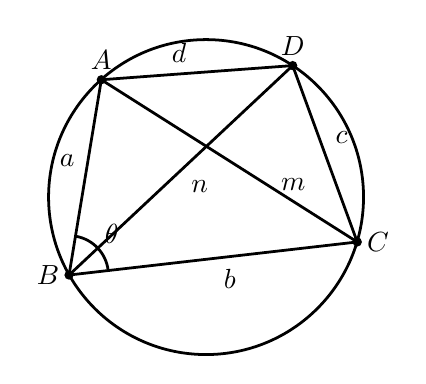
\begin{tikzpicture}[scale=1.0]
\coordinate[] (O) at (0,0);
\coordinate[label=left:$B$] (B) at (-1.74,-0.99);
\coordinate[label=$A$] (A) at (-1.33,1.49);
\coordinate[label=$D$] (D) at (1.1,1.67);
\coordinate[label=right:$C$] (C) at (1.92,-0.57);
\draw [line width=1pt] (O) circle (2cm);
\draw [line width=1pt] (A) to[edge label'=$a$](B);
\draw [line width=1pt] (B) to[edge label'=$b$](C);
\draw [line width=1pt] (C) to[edge label'=$c$](D);
\draw [line width=1pt] (D) to[edge label'=$d$](A);
\draw [line width=1pt] (A) -- (C) node [near end,above] {$m$};
\draw [line width=1pt] (B) to[edge label'=$n$] (D);
\foreach \p in {A,B,C,D}
	\fill[fill=black,draw=black,thick] (\p) circle (1.25pt);
\draw pic["$\theta$",draw,line width=1pt, angle eccentricity=1.5, angle radius=0.5cm] {angle=C--B--A};
\end{tikzpicture}
\end{figure*}

如图, 设 $AB=a, BC=b, CD=c, DA=d, AC=m, BD=n, \angle ABC=\theta$.

在 $\triangle ABC$ 和 $\triangle ADC$ 中, 由余弦定理有:
\begin{align*}
m^2 &= a^2+b^2-2ab\cos\theta \qquad\cdots\qquad \textcircled{1} \\
m^2 &= c^2+d^2+2cd\cos\theta \qquad\cdots\qquad \textcircled{2}
\end{align*}
由 $\textcircled{1}\times cd + \textcircled{2}\times ab$ 得:
\begin{align*} 
(ab+cd)m^2 &= cd(a^2+b^2)+ab(c^2+d^2) \\
&= (ac+bd)(ad+bc)
\end{align*}
于是
\[ m^2 = \frac{(ac+bd)(ad+bc)}{ab+cd} .\]
同理, 
\[n^2 =  \dfrac{(ac+bd)(ab+cd)}{ad+bc} .\]
相乘可得: $(mn)^2=(ac+bd)^2$. 所以 $AB\cdot CD+BC\cdot AD=AC\cdot BD$.

~

证法5: (面积法)

\begin{figure*}[htbp]
\centering
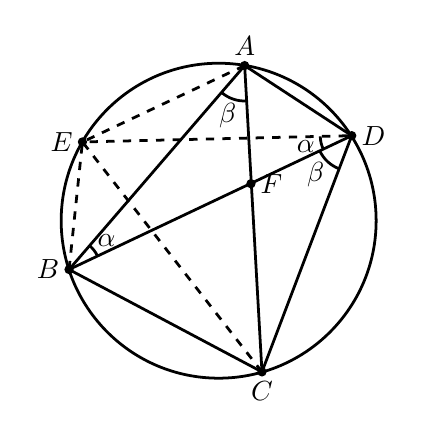
\begin{tikzpicture}[scale=1.0]
\coordinate[] (O) at (0,0);
\coordinate[label=$A$] (A) at (0.33,1.97);
\coordinate[label=left:$B$] (B) at (-1.9,-0.62);
\coordinate[label=below:$C$] (C) at (0.55,-1.92);
\coordinate[label=right:$D$] (D) at (1.69,1.08);
\coordinate[label=left:$E$] (E) at (-1.73,1.0);
\coordinate[label=right:$F$] (F) at (0.41,0.47);
\draw [line width=1pt] (O) circle (2cm);
\draw [line width=1pt] (A) -- (B) -- (C) -- (D) -- cycle;
\draw [line width=1pt] (A) -- (C);
\draw [line width=1pt] (B) -- (D);
\draw [dashed,line width=1pt] (A) -- (E) -- (B);
\draw [dashed,line width=1pt] (C) -- (E) -- (D);
\foreach \p in {A,B,C,D,E,F}
	\fill[fill=black,draw=black,thick] (\p) circle (1.25pt);
\draw pic["$\alpha$",draw,line width=1pt, angle eccentricity=1.5, angle radius=0.4cm] {angle=D--B--A};
\draw pic["$\alpha$",draw,line width=1pt, angle eccentricity=1.5, angle radius=0.4cm] {angle=E--D--B};
\draw pic["$\beta$",draw,line width=1pt, angle eccentricity=1.5, angle radius=0.45cm] {angle=B--A--C};
\draw pic["$\beta$",draw,line width=1pt, angle eccentricity=1.5, angle radius=0.45cm] {angle=B--D--C};
\end{tikzpicture}
\end{figure*}

如图, $AB,CD$的交点记为$F$, 作 $AE$ 平行于 $BD$ 交圆与 $E$ 点, 并连接 $BE, CE, DE$. 于是四边形 $AEBD$ 为等腰梯形, $EB = AD$. 图中相等得角用相同得希腊字母标出. 易知 $\angle AFD = \alpha+\beta=\angle EDC$.

记四边形$ABCD$的面积为 $S_1$, 四边形$EBCD$的面积为 $S_2$. 则
\begin{align*}
S_1 &= S_{\triangle ABD} + S_{\triangle BCD}\\
&= \frac{1}{2} BD \cdot AF \sin\angle AFD + \frac{1}{2} BD \cdot CF \sin\angle BFC\\
&= \frac{1}{2} BD\cdot AC \sin\angle AFD \\
&= \frac{1}{2} BD\cdot AC \sin\angle EDC \\
S_2 &= S_{\triangle EBC} + S_{\triangle EDC}\\
&= \frac{1}{2} EB \cdot BC \sin\angle EBC + \frac{1}{2} ED \cdot CD \sin\angle EDC
\end{align*}
因为 $\angle EBC$ 与 $\angle EDC$ 互补, 所以 $\sin\angle EBC = \sin\angle EDC$; 再由 $EB=AD$, $ED=AB$, 代入 $S_2$表达式得到:
\[ S_2 = \frac{1}{2}(AD\cdot BC + AB\cdot CD)\sin\angle EDC .\]

另一方面, $S_1 = S_{\triangle ABD} + S_{\triangle BCD} = S_{\triangle EBD} + S_{\triangle BCD} = S_2$, 所以 $AD\cdot BC + AB\cdot CD = AC\cdot BD$.

~

证法6: (无字证明)
\begin{figure*}[htbp]
\centering
\begin{minipage}[t]{0.4\linewidth}
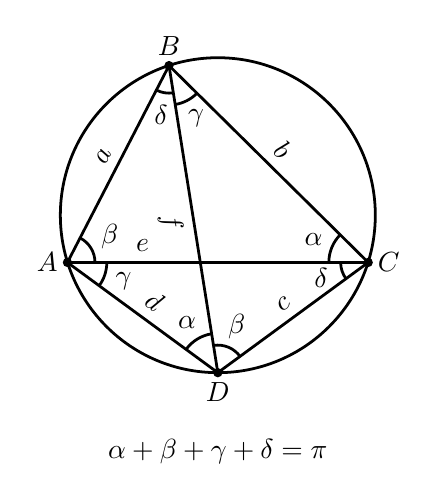
\begin{tikzpicture}[scale=1.0]
\coordinate[] (O) at (0,0);
\coordinate[label=left:$A$] (A) at (-1.91,-0.6);
\coordinate[label=above:$B$] (B) at (-0.62,1.9);
\coordinate[label=right:$C$] (C) at (1.91,-0.6);
\coordinate[label=below:$D$] (D) at (0,-2);
\draw [line width=1pt] (O) circle (2cm);
\draw [line width=1pt] (A) -- (B) node [midway,above,sloped] {$a$};
\draw [line width=1pt] (B) -- (C) node [midway,above,sloped] {$b$};
\draw [line width=1pt] (C) -- (D) node [midway,above,sloped] {$c$};
\draw [line width=1pt] (D) -- (A) node [midway,above,sloped] {$d$};
\draw [line width=1pt] (A) -- (C) node [near start,above,sloped] {$e$};
\draw [line width=1pt] (B) -- (D) node [midway,below,sloped] {$f$};
\foreach \p in {A,B,C,D}
	\fill[fill=black,draw=black,thick] (\p) circle (1.25pt);
\draw pic["$\beta$",draw,line width=1pt, angle eccentricity=1.8, angle radius=0.35cm] {angle=C--A--B};
\draw pic["$\beta$",draw,line width=1pt, angle eccentricity=1.8, angle radius=0.35cm] {angle=C--D--B};
\draw pic["$\delta$",draw,line width=1pt, angle eccentricity=1.8, angle radius=0.35cm] {angle=A--B--D};
\draw pic["$\delta$",draw,line width=1pt, angle eccentricity=1.8, angle radius=0.35cm] {angle=A--C--D};
\draw pic["$\alpha$",draw,line width=1pt, angle eccentricity=1.5, angle radius=0.5cm] {angle=B--D--A};
\draw pic["$\alpha$",draw,line width=1pt, angle eccentricity=1.5, angle radius=0.5cm] {angle=B--C--A};
\draw pic["$\gamma$",draw,line width=1pt, angle eccentricity=1.5, angle radius=0.5cm] {angle=D--B--C};
\draw pic["$\gamma$",draw,line width=1pt, angle eccentricity=1.5, angle radius=0.5cm] {angle=D--A--C};
\node at (0,-3.0) {$\alpha+\beta+\gamma+\delta=\pi$};
\end{tikzpicture}
\end{minipage}
\begin{minipage}[t]{0.5\linewidth}
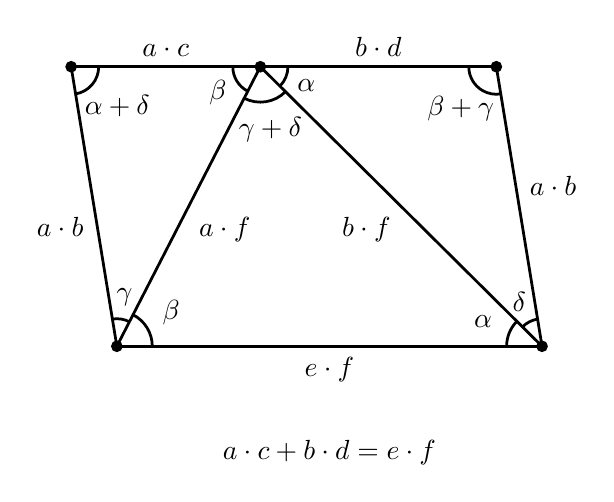
\begin{tikzpicture}[scale=1.35]
\coordinate[] (A) at (0,0);
\coordinate[] (B) at (4,0);
\coordinate[] (C) at (3.57,2.63);
\coordinate[] (D) at (-0.43,2.63);
\coordinate[] (E) at (1.35,2.63);
\draw [line width=1pt] (A) -- (B) node [midway,below,sloped] {$e\cdot f$};
\draw [line width=1pt] (B) to[edge label'=$a\cdot b$] (C);
\draw [line width=1pt] (C) -- (E) node [midway,above,sloped] {$b\cdot d$};
\draw [line width=1pt] (E) -- (D) node [midway,above,sloped] {$a\cdot c$};
\draw [line width=1pt] (D) to[edge label'=$a\cdot b$] (A);
\draw [line width=1pt] (A) to[edge label'=$a\cdot f$] (E);
\draw [line width=1pt] (E) to[edge label'=$b\cdot f$] (B);
\foreach \p in {A,B,C,D,E}
	\fill[fill=black,draw=black,thick] (\p) circle (1.25pt);
\draw pic["$\alpha+\delta$",draw,line width=1pt, angle eccentricity=2.2, angle radius=0.35cm] {angle=A--D--E};
\draw pic["$\beta$",draw,line width=1pt, angle eccentricity=1.8, angle radius=0.35cm] {angle=D--E--A};
\draw pic["$\gamma$",draw,line width=1pt, angle eccentricity=1.8, angle radius=0.35cm] {angle=E--A--D};
\draw pic["$\beta$",draw,line width=1pt, angle eccentricity=1.8, angle radius=0.45cm] {angle=B--A--E};
\draw pic["$\gamma+\delta$",draw,line width=1pt, angle eccentricity=1.8, angle radius=0.45cm] {angle=A--E--B};
\draw pic["$\alpha$",draw,line width=1pt, angle eccentricity=1.8, angle radius=0.45cm] {angle=E--B--A};
\draw pic["$\alpha$",draw,line width=1pt, angle eccentricity=1.8, angle radius=0.35cm] {angle=B--E--C};
\draw pic["$\delta$",draw,line width=1pt, angle eccentricity=1.8, angle radius=0.35cm] {angle=C--B--E};
\draw pic["$\beta+\gamma$",draw,line width=1pt, angle eccentricity=2.0, angle radius=0.35cm] {angle=E--C--B};
\node at (2,-1.0) {$a\cdot c+b\cdot d=e\cdot f$};
\end{tikzpicture}
\end{minipage}
\end{figure*}

~

证法7: (复数法)
\begin{figure*}[htbp]
\centering
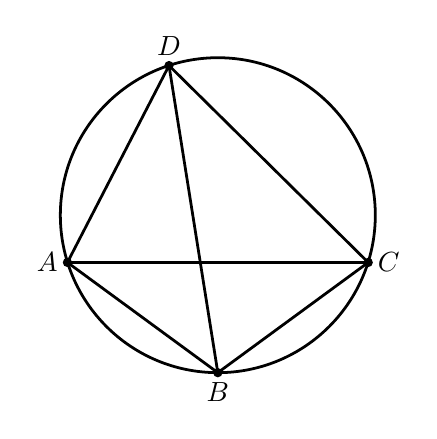
\begin{tikzpicture}[scale=1.0]
\coordinate[] (O) at (0,0);
\coordinate[label=left:$A$] (A) at (-1.91,-0.6);
\coordinate[label=above:$D$] (D) at (-0.62,1.9);
\coordinate[label=right:$C$] (C) at (1.91,-0.6);
\coordinate[label=below:$B$] (B) at (0,-2);
\draw [line width=1pt] (O) circle (2cm);
\draw [line width=1pt] (A) -- (B) -- (C) -- (D) -- cycle;
\draw [line width=1pt] (A) -- (C);
\draw [line width=1pt] (B) -- (D);
\foreach \p in {A,B,C,D}
	\fill[fill=black,draw=black,thick] (\p) circle (1.25pt);
\end{tikzpicture}
\end{figure*}

用 $a,b,c,d$ 分别表示 $A,B,C,D$ 的复数. 则
\begin{align*}
%overrightarrow
\vec{AB} &= b-a, \qquad \vec{AD} = d-a, \qquad \vec{AC} = c-a, \\
\vec{CD} &= d-c, \qquad \vec{BC} = c-b, \qquad \vec{BD} = d-b. 
\end{align*}
考虑到 
\begin{align*}
\angle DAB &= \arg\vec{AD}-\arg\vec{AB}\\
 &= \arg(d-a) - \arg(b-a)\\
\angle DCB &= 2\pi - (\arg\vec{CD} - \arg\vec{CB})\\
&= \arg(b-c)-\arg(d-c) + 2\pi
\end{align*}
由 $\angle DAB + \angle DCB = \pi$, 将上两式相加得:
\[\arg(d-a) - \arg(b-a) + \arg(b-c)-\arg(d-c) + \pi = 0\]
移项并注意到对于任意复数 $z$, $\arg(z)\pm\pi = \arg(-z)$, 得:
\[\arg(d-a) + \arg(c-b) = \arg(b-a) + \arg(d-c) \]
由辐角公式推出:
\[\arg[(d-a)(c-b)] = \arg[(b-a)(d-c)].\]
这表明两个复数$(d-a)(c-b)$和$(b-a)(d-c)$共线且同向, 于是模长之和等于和的模长:
\begin{align*}
|(b-a)(d-c)| + |(d-a)(c-b)| &= |(b-a)(d-c)+(d-a)(c-b)|\\
&= |(c-a)(d-b)|
\end{align*}
复数模长的乘积等于乘积的模长, 上面的等式就是
\[|\vec{AB}|\cdot|\vec{CD}| + |\vec{AD}|\cdot|\vec{BC}| = |\vec{AC}|\cdot|\vec{BD}|\]

~

证法8: (反演变换)
\begin{figure*}[htbp]
\centering
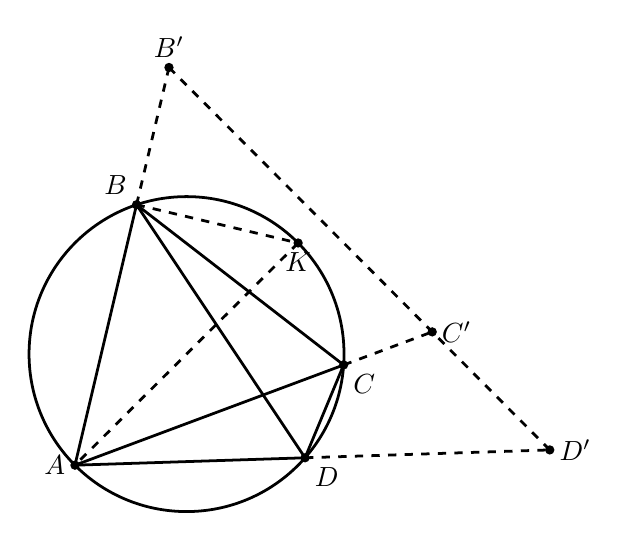
\begin{tikzpicture}[scale=1.0]
\coordinate[] (O) at (0,0);
\coordinate[label=left:$A$] (A) at (-1.417,-1.411);
\coordinate[label=above left:$B$] (B) at (-0.635,1.897);
\coordinate[label=below right:$C$] (C) at (1.995,-0.138);
\coordinate[label=below right:$D$] (D) at (1.505,-1.317);
\coordinate[label=above:$B'$] (BB) at (-0.223,3.64);
\coordinate[label=right:$C'$] (CC) at (3.12, 0.282);
\coordinate[label=right:$D'$] (DD) at (4.613, -1.217);
\coordinate[label=below:$K$] (K) at (1.417,1.411);
\draw [line width=1pt] (O) circle (2cm);
\draw [line width=1pt] (A) -- (B) -- (C) -- (D) -- cycle;
\draw [line width=1pt] (A) -- (C);
\draw [line width=1pt] (B) -- (D);
\draw [dashed,line width=1pt] (B) -- (BB);
\draw [dashed,line width=1pt] (C) -- (CC);
\draw [dashed,line width=1pt] (D) -- (DD);
\draw [dashed,line width=1pt] (BB) -- (DD);
\draw [dashed,line width=1pt] (B) -- (K) -- (A);
\foreach \p in {A,B,C,D,BB,CC,DD,K}
	\fill[fill=black,draw=black,thick] (\p) circle (1.25pt);
\end{tikzpicture}
\end{figure*}

对 $B,C,D$ 三点作反演变换, 反演的圆心为点 $A$, 半径为 1, 变换后得到的点为 $B', C', D'$. 则:
\[ AB\cdot AB'=AC\cdot AC'=AD\cdot AD'=1 \].
由余弦定理:
\begin{align*}
C'D' &= \sqrt{AC'^2 + AD'^2 - 2AC'\cdot AD'\cos\angle CAD}\\
&= \sqrt{AC^2 + AD^2-2AC\cdot AD\cos\angle CAD}\cdot\left(\frac{1}{AC}\cdot\frac{1}{AD}\right)\\
&= \frac{CD}{AC\cdot AD} .
\end{align*}
同理可得: \[B'C' = \dfrac{BC}{AB\cdot AC}, B'D'=\dfrac{BD}{AB\cdot AD} .\]
因为 $A,B,C,D$ 共圆, 所以 $B',C',D'$共线, 于是有: $B'C'+C'D'=B'D'$, 即:
\[\frac{BC}{AB\cdot AC}+\frac{CD}{AC\cdot AD} = \frac{BD}{AB\cdot AD}.\]
两边都乘以 $AB\cdot AC\cdot AD$ 得: $BC\cdot AD+ AB\cdot CD = BD\cdot AC$.

~

补充: 类似的思路, 但不需要用反演的性质, 可以用向量的方法, 在 $AB, AC, AD$的延长线上分别取  $B',C',D'$, 满足 $\vec{AB}\cdot\vec{AB'}=\vec{AC}\cdot\vec{AC'}=\vec{AD}\cdot\vec{AD'}=1$. 下面证明 $B',C',D'$ 共线. 

设 $AK$ 是圆 $ABCD$ 的直径, 则$AB\perp BK$, 向量 $\vec{AK}$ 在 $AB$ 上的投影就是 $\vec{AB}$, 故 $\vec{AK}\cdot\vec{AB'}=1$. 同理也有 $\vec{AK}\cdot\vec{AC'}=\vec{AK}\cdot\vec{AD'}=1$. 于是有 $\vec{AK}\cdot(\vec{AC'}-\vec{AB'}) = \vec{AK}\cdot\vec{B'C'} = 0$ 和 $\vec{AK}\cdot(\vec{AD'}-\vec{AC'}) = \vec{AK}\cdot\vec{C'D'} = 0$, 说明 $\vec{B'C'}, \vec{C'D'}$ 都垂直于 $\vec{AK}$, 所以 $B'C'D'$ 共线. 

剩余部分用反演法中的余弦定理往下推导即可.

~

证法9: (向量法)
\begin{figure*}[htbp]
\centering
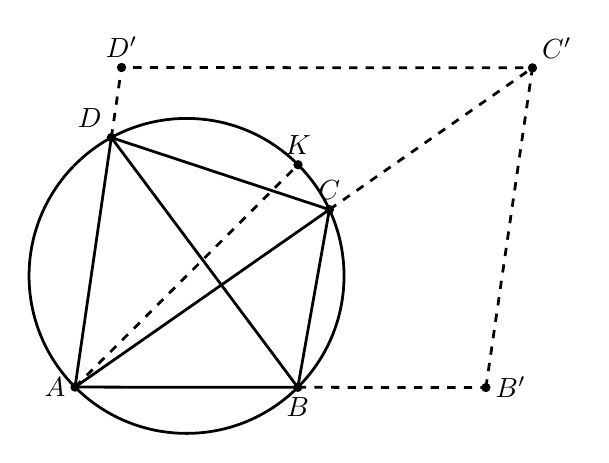
\begin{tikzpicture}[scale=1.0]
\coordinate[] (O) at (0,0);
\coordinate[label=left:$A$] (A) at (-1.416,-1.412);
\coordinate[label=below:$B$] (B) at (1.413,-1.415);
\coordinate[label=above:$C$] (C) at (1.814,0.842);
\coordinate[label=above left:$D$] (D) at (-0.955,1.757);
\coordinate[label=right:$B'$] (BB) at (3.802,-1.418);
\coordinate[label=above right:$C'$] (CC) at (4.393, 2.642);
\coordinate[label=above:$D'$] (DD) at (-0.825, 2.647);
\coordinate[label=above:$K$] (K) at (1.416,1.412);
\draw [line width=1pt] (O) circle (2cm);
\draw [line width=1pt] (A) -- (B) -- (C) -- (D) -- cycle;
\draw [line width=1pt] (A) -- (C);
\draw [line width=1pt] (B) -- (D);
\draw [dashed,line width=1pt] (B) -- (BB);
\draw [dashed,line width=1pt] (C) -- (CC);
\draw [dashed,line width=1pt] (D) -- (DD);
\draw [dashed,line width=1pt] (BB) -- (CC) -- (DD);
\draw [dashed,line width=1pt] (A) -- (K);
\foreach \p in {A,B,C,D,BB,CC,DD,K}
	\fill[fill=black,draw=black,thick] (\p) circle (1.25pt);
\end{tikzpicture}
\end{figure*}

在 $AB, AC, CD$ 上各取一点 $B',C',D'$, 使得$AB'C'D'$是平行四边形. 由 $\angle C'AB' = \angle CDB$ 和 $\angle AC'B' = \angle C'AD = \angle DBC$, 得 $\triangle C'AB'\sim\triangle BDC$, 所以
\[\frac{|\vec{BD}|}{|\vec{AC'}|} = \frac{|\vec{CD}|}{|\vec{AB'}|} = \frac{|\vec{BC}|}{|\vec{B'C'}|} \qquad\cdots\qquad \textcircled{1}.\]

设 $AK$ 是圆的直径, 所以$\vec{AK}$ 在$AB,AC,AD$上的投影分别是$\vec{AB},\vec{AC},\vec{AD}$, 于是
\begin{align*}
\vec{AC}\cdot\vec{AC'} &= \vec{AF}\cdot\vec{AC'} = \vec{AK}\cdot(\vec{AB'}+\vec{AD'})\\
&= \vec{AK}\cdot\vec{AB'}+\vec{AK}\cdot\vec{AD'}\\
&= \vec{AB}\cdot\vec{AB'}+\vec{AD}\cdot\vec{AD'}
\end{align*}
即: \[|\vec{AC}|\cdot|\vec{AC'}| = |\vec{AB}|\cdot|\vec{AB'}| + |\vec{AD}|\cdot|\vec{AD'}| .\]
上式乘以$\textcircled{1}$式得: 
\[|\vec{AC}|\cdot|\vec{AC'}|\cdot\frac{|\vec{BD}|}{|\vec{AC'}|} = |\vec{AB}|\cdot|\vec{AB'}|\cdot\frac{|\vec{CD}|}{|\vec{AB'}|} + |\vec{AD}|\cdot|\vec{AD'}|\cdot\frac{|\vec{BC}|}{|\vec{B'C'}|} .\]
注意到 $\vec{B'C'}=\vec{AD'}$, 所以 $|\vec{AC}|\cdot|\vec{BD}| = |\vec{AB}|\cdot|\vec{CD}|+|\vec{AD}|\cdot|\vec{BC}|$.

~

证法10: (坐标解析法, 本质是正弦定理)
\begin{figure*}[htbp]
\centering
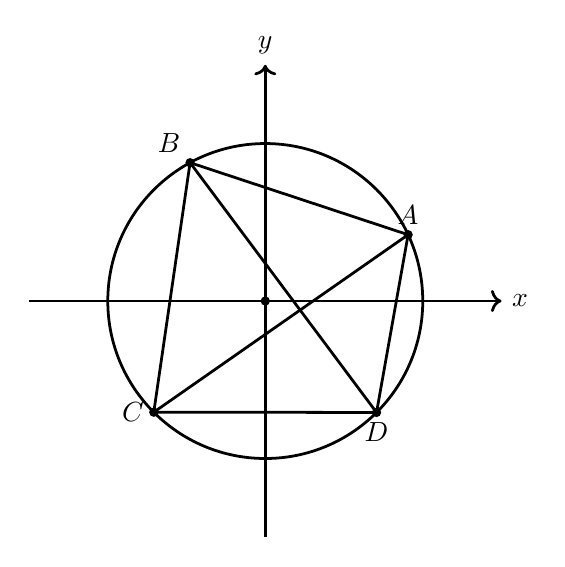
\begin{tikzpicture}[scale=1.0]
\tikzstyle{axes}=[line width=1pt]
\coordinate[] (O) at (0,0);
\coordinate[label=above:$A$] (A) at (1.814,0.842);
\coordinate[label=above left:$B$] (B) at (-0.955,1.757);
\coordinate[label=left:$C$] (C) at (-1.416,-1.412);
\coordinate[label=below:$D$] (D) at (1.413,-1.415);
\draw [line width=1pt] (O) circle (2cm);
\draw [line width=1pt] (A) -- (B) -- (C) -- (D) -- cycle;
\draw [line width=1pt] (A) -- (C);
\draw [line width=1pt] (B) -- (D);
\begin{scope}[style=axes]
    \draw[->] (-3,0) -- (3,0) node[right] {$x$};
    \draw[->] (0,-3) -- (0,3) node[above] {$y$};
\end{scope}
\foreach \p in {A,B,C,D,O}
	\fill[fill=black,draw=black,thick] (\p) circle (1.25pt);
\end{tikzpicture}
\end{figure*}

设圆的半径为1, $A,B,C,D$ 四点的坐标分别是 $A=(\cos\alpha,\sin\alpha)$, $B=(\cos\beta,\sin\beta)$, $C=(\cos\gamma,\sin\gamma)$, $D=(\cos\delta,\sin\delta)$, 其中 $\alpha<\beta<\gamma<\delta$. 由正弦定理可得: 
\begin{align*}
|AB| &= 2\sin(\frac{\beta-\alpha}{2}),\qquad |CD| = 2\sin(\frac{\delta-\gamma}{2}), \\
|AD| &= 2\sin(\frac{\delta-\alpha}{2}), \qquad |BC| = 2\sin(\frac{\gamma-\beta}{2}),\\
|AC| &= 2\sin(\frac{\gamma-\alpha}{2}), \qquad |BD| = 2\sin(\frac{\delta-\beta}{2}).
\end{align*}
进而:
\begin{align*}
&|AB|\cdot|CD|+|AD|\cdot|BC| \\
=& 4\sin(\frac{\beta-\alpha}{2})\sin(\frac{\delta-\gamma}{2}) + 4\sin(\frac{\delta-\alpha}{2})\sin(\frac{\gamma-\beta}{2}) \\
=& 2\cos(\frac{\beta-\alpha-\delta+\gamma}{2}) - 2\cos(\frac{\delta-\alpha+\gamma-\beta}{2})\\
=&4\sin(\frac{\gamma-\alpha}{2})\sin(\frac{\delta-\beta}{2})\\
=&|AC|\cdot|BD|
\end{align*}

~

证法11: (反演变换2.0)
\begin{figure*}[htbp]
\centering
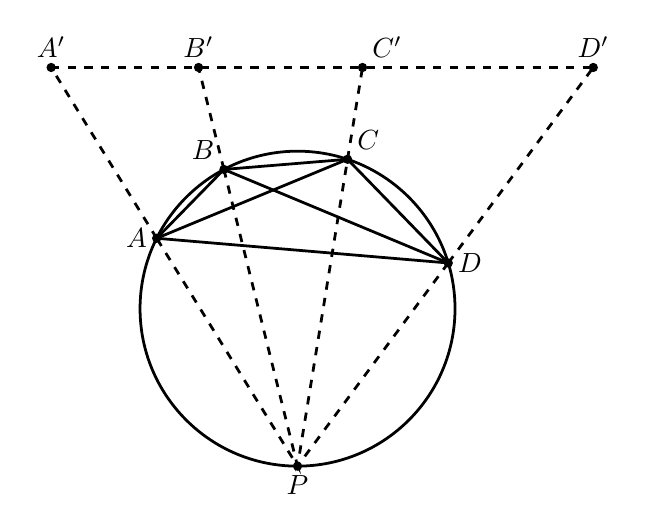
\begin{tikzpicture}[scale=1.0]
\coordinate[] (O) at (0,0);
\coordinate[label=left:$A$] (A) at (-1.789,0.894);
\coordinate[label=above left:$B$] (B) at (-0.935,1.768);
\coordinate[label=above right:$C$] (C) at (0.635,1.897);
\coordinate[label=right:$D$] (D) at (1.914,0.58);
\coordinate[label=above:$A'$] (AA) at (-3.129,3.063);
\coordinate[label=above:$B'$] (BB) at (-1.257,3.063);
\coordinate[label=above right:$C'$] (CC) at (0.825, 3.063);
\coordinate[label=above:$D'$] (DD) at (3.756, 3.063);
\coordinate[label=below:$P$] (P) at (0, -2);
\draw [line width=1pt] (O) circle (2cm);
\draw [line width=1pt] (A) -- (B) -- (C) -- (D) -- cycle;
\draw [line width=1pt] (A) -- (C);
\draw [line width=1pt] (B) -- (D);
\draw [dashed,line width=1pt] (B) -- (P) -- (A);
\draw [dashed,line width=1pt] (D) -- (P) -- (C);
\draw [dashed,line width=1pt] (A) -- (AA);
\draw [dashed,line width=1pt] (B) -- (BB);
\draw [dashed,line width=1pt] (C) -- (CC);
\draw [dashed,line width=1pt] (D) -- (DD);
\draw [dashed,line width=1pt] (AA) -- (BB) -- (CC) -- (DD);
\foreach \p in {A,B,C,D,AA,BB,CC,DD,P}
	\fill[fill=black,draw=black,thick] (\p) circle (1.25pt);
\end{tikzpicture}
\end{figure*}

在圆上取不同于 $A,B,C,D$ 的一点 $P$, 对$A,B,C,D$分别作反演变换, 反演中心为 $P$, 半径为 1. 则
\[ PA\cdot PA'=PB\cdot PB'=PC\cdot PC'=PD\cdot PD'=1 .\]
考虑 $\triangle PAB$ 和 $\triangle PB'A'$, 因为 $PA:PB = PB':PA'$, 再加上一个公共角 $\angle A'PB'=\angle BPA$, 所以 $\triangle PAB \sim \triangle PB'A'$, 故 $A'B':BA = PA':PB$, 于是
\[ A'B' = \frac{AB\cdot PA'}{PB} = \frac{AB}{PA\cdot PB} .\]
同理还有
\begin{align*}
A'C' &= \frac{AC}{PA\cdot PC}, \qquad A'D' = \frac{AD}{PA\cdot PD}, \qquad B'C' = \frac{BC}{PB\cdot PC}\\
C'D' &= \frac{CD}{PC\cdot PD}, \qquad B'D' = \frac{BD}{PB\cdot PD} .
\end{align*}
由反演性质知$A',B',C',D'$共线, 所以
\begin{align*}
A'C'\cdot B'D' &= (A'B'+B'C')\cdot(B'C'+C'D')\\
&=A'B'\cdot C'D'+B'C'\cdot(A'B'+B'C'+C'D')\\
&=A'B'\cdot C'D'+B'C'\cdot A'D'
\end{align*}
将上面各式代入后, 并约去分母, 得到: $AC\cdot BD = AB\cdot CD+BC\cdot AD$.

~

证法12: (余弦定理)
\begin{figure*}[htbp]
\centering
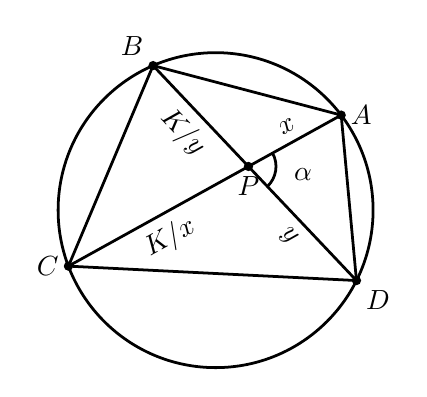
\begin{tikzpicture}[scale=1.0]
\coordinate[] (O) at (0,0);
\coordinate[label=right:$A$] (A) at (1.595,1.207);
\coordinate[label=above left:$B$] (B) at (-0.794,1.836);
\coordinate[label=left:$C$] (C) at (-1.869,-0.711);
\coordinate[label=below right:$D$] (D) at (1.789,-0.894);
\coordinate[label=below:$P$] (P) at (0.417,0.555);
\draw [line width=1pt] (O) circle (2cm);
\draw [line width=1pt] (A) -- (B) -- (C) -- (D) -- cycle;
\draw [line width=1pt] (A) -- (P) node [midway,above,sloped] {$x$};
\draw [line width=1pt] (P) -- (C) node [midway,below,sloped] {$K/x$};
\draw [line width=1pt] (B) -- (P) node [midway,below,sloped] {$K/y$};
\draw [line width=1pt] (P) -- (D)  node [midway,below,sloped] {$y$};
\foreach \p in {A,B,C,D,P}
	\fill[fill=black,draw=black,thick] (\p) circle (1.25pt);
\draw pic["$\alpha$",draw,line width=1pt, angle eccentricity=2.0, angle radius=0.35cm] {angle=D--P--A};
\end{tikzpicture}
\end{figure*}

设 $AC, BD$ 交于 $P$ 点, $\angle APD = \alpha$. 设 $PA=x, PD=y$, 由圆幂定理得
\[PA\cdot PC = PB\cdot PD = K, \]
于是 $PB = \dfrac{K}{y}, PC = \dfrac{K}{x}$. 由余弦定理:
\begin{align*}
AD &= \sqrt{x^2+y^2-2xy\cdot\cos\alpha}\\
BC &= \frac{K}{xy}\sqrt{x^2+y^2-2xy\cdot\cos\alpha}\\
AB &= \sqrt{x^2+\frac{K^2}{y^2}+2x\cdot\frac{K}{y}\cdot\cos\alpha}\\
CD &= \frac{y}{x}\sqrt{x^2+\frac{K^2}{y^2}+2x\cdot\frac{K}{y}\cdot\cos\alpha}\\
AC&= x + \frac{K}{x} , \qquad BD = y + \frac{K}{y}
\end{align*}
进而:
\begin{align*}
AB\cdot CD &= \frac{y}{x}(x^2+\frac{K^2}{y^2}+2x\cdot\frac{K}{y}\cdot\cos\alpha) = xy+\frac{K^2}{xy}+2K\cdot\cos\alpha\\
AD\cdot BC &= \frac{K}{xy}(x^2+y^2-2xy\cdot\cos\alpha) = \frac{Kx}{y} + \frac{Ky}{x}-2K\cdot\cos\alpha \\
AB\cdot CD + AD\cdot BC &= K\cdot\frac{x}{y} + K\cdot\frac{y}{x} + xy + \frac{K^2}{xy}\\
&= (x+\frac{K}{x})(y+\frac{K}{y})\\
&= AC\cdot BD
\end{align*}

~

证法13: (函数求导)
\begin{figure*}[htbp]
\centering
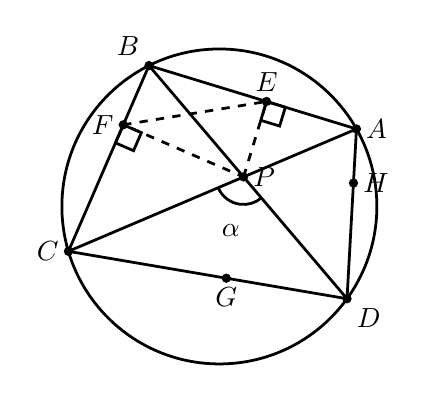
\begin{tikzpicture}[scale=1.0]
\coordinate[] (O) at (0,0);
\coordinate[label=right:$A$] (A) at (1.741,0.984);
\coordinate[label=above left:$B$] (B) at (-0.894,1.789);
\coordinate[label=left:$C$] (C) at (-1.917,-0.57);
\coordinate[label=below right:$D$] (D) at (1.621,-1.172);
\coordinate[label=above:$E$] (E) at (0.599,1.333);
\coordinate[label=left:$F$] (F) at (-1.22,1.037);
\coordinate[label=below:$G$] (G) at (0.088,-0.911);
\coordinate[label=right:$H$] (H) at (1.703,0.297);
\coordinate[label=right:$P$] (P) at (0.307,0.375);
\draw [line width=1pt] (O) circle (2cm);
\draw [line width=1pt] (A) -- (B) -- (C) -- (D) -- cycle;
\draw [line width=1pt] (A) -- (C);
\draw [line width=1pt] (B) -- (D);
\draw [dashed,line width=1pt] (P) -- (E) -- (F) -- cycle;
\foreach \p in {A,B,C,D,E,F,G,H,P}
	\fill[fill=black,draw=black,thick] (\p) circle (1.25pt);
\draw pic["$\alpha$",draw,line width=1pt, angle eccentricity=2.0, angle radius=0.35cm] {angle=C--P--D};
\tkzMarkRightAngle[line width=1pt](P,E,A);
\tkzMarkRightAngle[line width=1pt](P,F,C);
\end{tikzpicture}
\end{figure*}

设 $AC, BD$ 的交点为 $P$, 固定 $PA,PB,PC,PD$ 的长度, $AC$ 不动, $BD$ 绕着 $P$ 点旋转, 因为恒有 $PA\cdot PC = PB\cdot PD$, 所以 $A,B,C,D$ 四点总是共圆的. 过 $P$ 点作 $AB,BC,CD,DA$ 的垂线, 垂足分别为 $E,F,G,H$.

设 $\angle APB = \alpha$, 则四条边 $AB,BC,CD,DA$ 的长度各自是 $\alpha$ 的一元函数. 例如
\[ AB^2 = PA^2 + PB^2 - 2PA\cdot PB\cdot\cos\alpha .\]
两边对 $\alpha$ 求导:
\[2AB\cdot AB'(\alpha) = 2PA\cdot PB\sin\alpha ,\]
即 $AB'(\alpha) = \dfrac{PA\cdot PB\sin\alpha}{AB}$, 说明 $AB'(\alpha)$ 等于 $P$ 到 $AB$ 的距离, 即 $AB'(\alpha) = PE$. 

同理, $CD'(\alpha)=PG$. $PB$与$PC$的夹角为 $\pi-\alpha$, 容易得到 $BC'(\alpha)=-PF, AD'(\alpha)=PH$.
最后, $AC$ 和 $BD$ 的长度不随 $\alpha$ 变化, 所以 $AC'(\alpha)=BD'(\alpha)=0$.

令 $f(\alpha) = AB\cdot CD + AD\cdot BC - AC\cdot BD$, 则
\begin{align*} f' &= AB'\cdot CD +AB\cdot CD'+ AD'\cdot BC +AD\cdot BC' - AC'\cdot BD-AC\cdot BD'\\
&= PE\cdot CD + AB\cdot PG - PH\cdot BC - AD\cdot PF
\end{align*}
由 $\triangle ABP \sim \triangle DCP$, 得 $PE:PG = AB:CD$, 即 $PE\cdot CD = PG\cdot AB$. 同理由 $\triangle BCP \sim \triangle ADP$, 可得 $PF\cdot AD = PH\cdot BC$. 于是
\[ f' = 2(PE\cdot CD - PF\cdot AD) .\]
考虑四边形 $PEBF$, 因为有一组对角都是直角, 所以 $P,E,B,F$ 四点共圆, 由 $\angle EFP = \angle ADB = \angle ACD$, 以及 $\angle FEP = \angle CBD = \angle CAD$, 推出 $\triangle EFP\sim\triangle ACD$, 于是 $PE\cdot CD = PF\cdot AD$. 这说明 $f'(\alpha) = 0$, 所以 $f(\alpha)$ 不随 $\alpha$ 变化.

特别地, 取 $\alpha = 0$, 则 $A,B,C,D$ 共线, 沿着$C$到 $A$ 方向上四个点经过的顺序依次是 $C,D,A,B$, 所以
\begin{align*}
f(0) &= AB\cdot CD + AD\cdot BC - AC\cdot BD\\
&= AB\cdot CD + AD\cdot(CD+AD+AB) - (CD+AD)\cdot(AD+AB)
&=0
\end{align*}
这就证明了 $AB\cdot CD + AD\cdot BC = AC\cdot BD$.

~

证法14: (面积法 2.0)
\begin{figure*}[htbp]
\centering
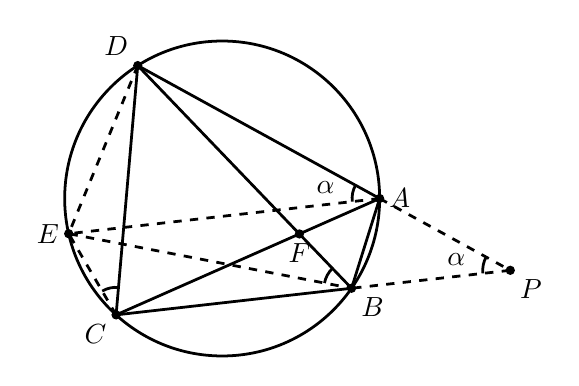
\begin{tikzpicture}[scale=1.0]
\coordinate[] (O) at (0,0);
\coordinate[label=right:$A$] (A) at (2,0);
\coordinate[label=below right:$B$] (B) at (1.643,-1.14);
\coordinate[label=below left:$C$] (C) at (-1.347,-1.478);
\coordinate[label=above left:$D$] (D) at (-1.072,1.688);
\coordinate[label=left:$E$] (E) at (-1.949,-0.447);
\coordinate[label=below:$F$] (F) at (0.981,-0.45);
\coordinate[label=below right:$P$] (P) at (3.659,-0.912);
\draw [line width=1pt] (O) circle (2cm);
\draw [line width=1pt] (A) -- (B) -- (C) -- (D) -- cycle;
\draw [line width=1pt] (A) -- (C);
\draw [line width=1pt] (B) -- (D);
\draw [dashed,line width=1pt] (A) -- (E) -- (C);
\draw [dashed,line width=1pt] (A) -- (P) -- (B);
\draw [dashed,line width=1pt] (D) -- (E) -- (B);
\foreach \p in {A,B,C,D,E,F,P}
	\fill[fill=black,draw=black,thick] (\p) circle (1.25pt);
\draw pic["$\alpha$",draw,line width=1pt, angle eccentricity=2.0, angle radius=0.35cm] {angle=A--P--B};
\draw pic["$\alpha$",draw,line width=1pt, angle eccentricity=2.0, angle radius=0.35cm] {angle=D--A--E};
\draw pic[draw,line width=1pt, angle eccentricity=2.0, angle radius=0.35cm] {angle=D--B--E};
\draw pic[draw,line width=1pt, angle eccentricity=2.0, angle radius=0.35cm] {angle=D--C--E};
\end{tikzpicture}
\end{figure*}

过 $A$ 作 $AE$ 平行于 $BC$, 交圆于 $E$ 点, 连接 $BE, CE, DE$, 设 $BC$ 与 $AD$ 交于 $P$ 点, $AC$与$BD$交于 $F$ 点, $\angle APB  = \alpha$. 

四边形 $ABCE$ 为等腰梯形, $AB= EC, AC=EB$. 在 $\triangle ABC$ 中, $BC$ 边上的高为 $AP\cdot\sin\alpha$, 而对于 $\triangle DBC$, $BC$ 边上的高为 $DP\cdot\sin\alpha$, 所以
\begin{align*}
\frac{1}{2}\cdot AD\cdot BC\cdot\sin\alpha &= \frac{1}{2}\cdot (DP-AP)\cdot BC\sin\alpha \\
&= S_{\triangle DCB} - S_{\triangle ACB}\\
&=S_{\triangle DCB} - S_{\triangle ECB}\\
& = S_{\triangle DBE} - S_{\triangle DCE}
\end{align*}
而 $\angle APB = \angle DAE = \angle DBE = \angle DCE = \alpha$, 所以
\begin{align*}
S_{\triangle DBE} &= \frac{1}{2}\cdot BD\cdot BE\cdot\sin\angle DBE = \frac{1}{2}\cdot BD\cdot AC\cdot\sin\alpha\\
S_{\triangle DCE} &= \frac{1}{2}\cdot CE\cdot CD\cdot\sin\angle DCE = \frac{1}{2}\cdot AB\cdot CD\cdot\sin\alpha
\end{align*}
将它们代入前面得式子, 并约去 $\dfrac{1}{2}\sin\alpha$, 得: $AD\cdot BD = AC\cdot BD - AB\cdot BD$.

~

证法15: (西姆松线)

先证明引理(西姆松定理): 过三角形外接圆上异于三角形顶点得任意一点, 作三条边或其延长线的垂线, 则三个垂足共线.
\begin{figure*}[htbp]
\centering
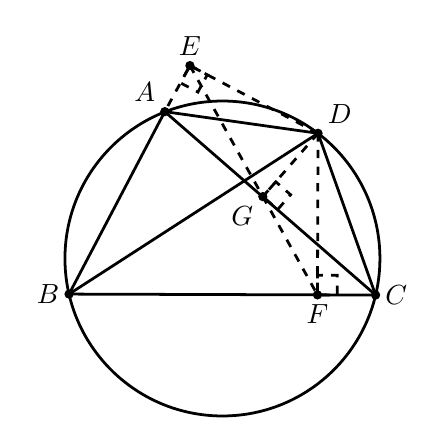
\begin{tikzpicture}[scale=1.0]
\coordinate[] (O) at (0,0);
\coordinate[label=above left:$A$] (A) at (-0.732,1.865);
\coordinate[label=left:$B$] (B) at (-1.948,-0.452);
\coordinate[label=right:$C$] (C) at (1.945,-0.464);
\coordinate[label=above right:$D$] (D) at (1.214,1.59);
\coordinate[label=above:$E$] (E) at (-0.413,2.45);
\coordinate[label=below:$F$] (F) at (1.207,-0.462);
\coordinate[label=below left:$G$] (G) at (0.513,0.786);
\draw [line width=1pt] (O) circle (2cm);
\draw [line width=1pt] (A) -- (B) -- (C) -- (D) -- cycle;
\draw [line width=1pt] (A) -- (C);
\draw [line width=1pt] (B) -- (D);
\draw [dashed,line width=1pt] (D) -- (E) -- (A);
\draw [dashed,line width=1pt] (D) -- (F);
\draw [dashed,line width=1pt] (D) -- (G);
\draw [dashed,line width=1pt] (E) -- (G) -- (F);
\foreach \p in {A,B,C,D,E,F,G}
	\fill[fill=black,draw=black,thick] (\p) circle (1.25pt);
\tkzMarkRightAngle[dashed,line width=1pt](D,E,A);
\tkzMarkRightAngle[dashed,line width=1pt](D,G,C);
\tkzMarkRightAngle[dashed,line width=1pt](D,F,C);
\end{tikzpicture}
\end{figure*}

由四边形包含一组相对的顶角是直角, 可以得到三个顶点共圆的四边形, 分别是 $BFDE$, $AGDE$, 和 $CDGF$.

在四边形 $BFDE$ 中, $\angle FDE = 180\degree - \angle ABC$, 而 在四边形 $ABCD$ 中, $\angle ADC = 180\degree - \angle ABC$, 于是 $\angle FDE = \angle ADC$. 减去重叠的角度, 有 $\angle ADE = \angle CDF$.

再由$C,D,F,G$共圆知: $\angle CDF = \angle CGF$; 由 $A,G,D,E$ 共圆知: $\angle ADE = \angle AGE$. 所以 $\angle AGE = \angle CGF$. 这说明 $GE$ 和 $GF$ 在一条直线上, 故 $E,F,G$三点共线.

回到托勒密定理, 由正弦定理得:
\begin{align*}
EG &= AD\cdot\sin\angle GDE\\
GF &= CD\cdot\sin\angle GCF\\
EF &= BD\cdot\sin\angle EBF
\end{align*}
设四边形 $ABCD$ 的外接圆半径为 $2R$, 那么
\begin{align*}
\sin\angle GDE &= \sin\angle GAE = \sin\angle BAC = \frac{BC}{2R}\\
\sin\angle GCF &= \frac{AB}{2R}\\
\sin\angle EBF &= \frac{AC}{2R}
\end{align*}
代入前面的三个等式, 并根据 $EF = EG + GF$, 得
\[BD\cdot\frac{AC}{2R} = AD\cdot\frac{BC}{2R} + CD\cdot\frac{AB}{2R} ,\]
即: $BD\cdot AC = AD\cdot BC + AB\cdot CD$ . 

%------------------------------------------------------------------------------%
\newpage
圆幂, 根轴, 根心, 蒙日定理

圆幂定理: 过一定点 $P$ 作任意直线, 与半径为 $R$ 的圆 $O$ 交于两点$A,B$, 则 $PA$ 与 $PB$ 长度的乘积是定值, 恒为 $|OP^2 - R^2|$, 而 $OP^2 - R^2$ 称为点 $P$ 对于圆 $O$ 的圆幂, 圆内的点的幂为负数,圆外的点的幂为正数,圆上的点的幂为零. 

圆幂定理是对相交弦定理, 切割线定理及割线定理的总结. 

\begin{figure*}[htbp]
\centering
\begin{minipage}[t]{0.4\linewidth}
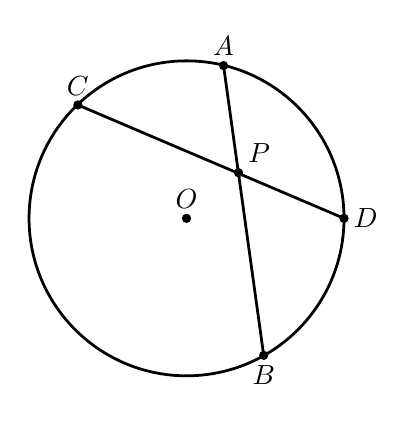
\begin{tikzpicture}[scale=1]
\coordinate[label=$O$] (O) at (0,0);
\coordinate[label=$A$] (A) at (0.47,1.94);
\coordinate[label=$C$] (C) at (-1.38,1.44);
\coordinate[label=below:$B$] (B) at (0.98,-1.74);
\coordinate[label=right:$D$] (D) at (2,0);
\coordinate[label=above right:$P$] (P) at (0.66,0.58);
\coordinate[] (E) at (1.5,1.32);
\coordinate[] (F) at (-1.5,-1.32);
\draw [line width=1pt] (O) circle (2cm);
\draw [line width=1pt] (A) to (B);
\draw [line width=1pt] (C) to (D);
\foreach \p in {O,A,B,C,D,P}
	\fill[fill=black,draw=black,thick] (\p) circle (1.25pt);
\end{tikzpicture}
\end{minipage}
\begin{minipage}[t]{0.4\linewidth}
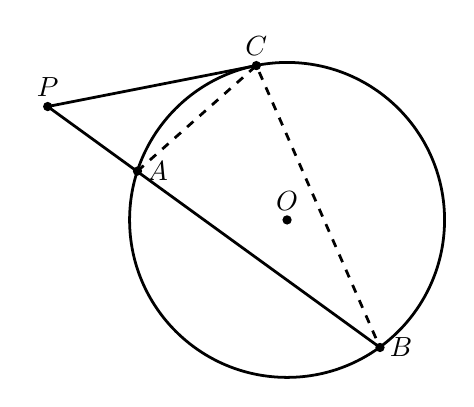
\begin{tikzpicture}[scale=1]
\coordinate[label=$O$] (O) at (0,0);
\coordinate[label=$C$] (C) at (-0.39,1.96);
\coordinate[label=$P$] (P) at (-3.04,1.44);
\coordinate[label=right:$A$] (A) at (-1.9,0.62);
\coordinate[label=right:$B$] (B) at (1.18,-1.62);
\draw [line width=1pt] (O) circle (2cm);
\draw [line width=1pt] (P) to (C);
\draw [line width=1pt] (P) to (B);
\draw [dashed,line width=1pt] (A) -- (C) -- (B);
\foreach \p in {O,A,B,C,P}
	\fill[fill=black,draw=black,thick] (\p) circle (1.25pt);
\end{tikzpicture}
\end{minipage}
\end{figure*}

相交弦定理: 过圆 $O$ 内一点 $P$ 作圆的两个弦 $AB$ 和 $CD$, 则 $PA\cdot PB = PC\cdot PD = (R-OP)(R+OP)$.

切割线定理: 过圆 $O$ 外一点 $P$ 作圆的切线和割线, 割线交圆于 $A,B$ 两点, 而切线的切点为 $C$, 则 $PC^2=PA\cdot PB$.

割线定理: 过圆 $O$ 外一点 $P$ 作圆的两条割线$AB$和$CD$, 则 $PA\cdot PB = PC\cdot PD$. 它们都等于过$P$点的切线长的平方.

根轴: 到固定两圆的圆幂相等的点组成的直线为这两圆的根轴, 这条根轴垂直于连心线.
\begin{figure*}[htbp]
\centering
\begin{minipage}[t]{0.45\linewidth}
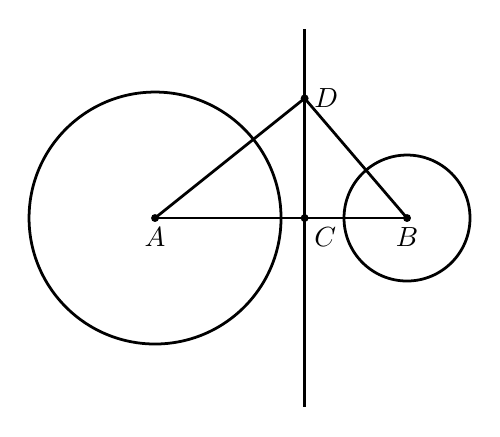
\begin{tikzpicture}[scale=0.8]
\coordinate[label=below:$A$] (A) at (0.0,0.0);
\coordinate[label=below:$B$] (B) at (4.0,0.0);
\coordinate[label=below right:$C$] (C) at (2.375,0);
\coordinate[label=right:$D$] (D) at (2.375,1.9);
\coordinate[] (E) at (2.375,3);
\coordinate[] (F) at (2.375,-3);
\draw [line width=1pt] (A) circle (2cm);
\draw [line width=1pt] (B) circle (1cm);
\draw [line width=1pt] (A) to (B);
\draw [line width=1pt] (E) to (F);
\draw [line width=1pt] (A) -- (D) -- (B);
\foreach \p in {A,B,C,D}
	\fill[fill=black,draw=black,thick] (\p) circle (1.25pt);
\end{tikzpicture}
\end{minipage}
\begin{minipage}[t]{0.45\linewidth}
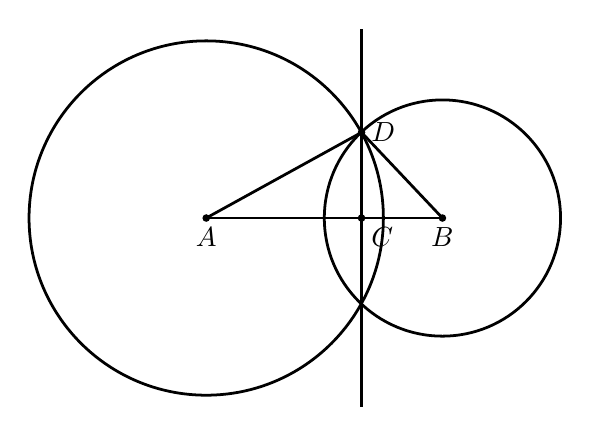
\begin{tikzpicture}[scale=0.75]
\coordinate[label=below:$A$] (A) at (0.0,0.0);
\coordinate[label=below:$B$] (B) at (4.0,0.0);
\coordinate[label=below right:$C$] (C) at (2.63,0);
\coordinate[label=right:$D$] (D) at (2.63,1.45);
\coordinate[] (E) at (2.63,3.2);
\coordinate[] (F) at (2.63,-3.2);
\draw [line width=1pt] (A) circle (3cm);
\draw [line width=1pt] (B) circle (2cm);
\draw [line width=1pt] (A) to (B);
\draw [line width=1pt] (E) to (F);
\draw [line width=1pt] (A) -- (D) -- (B);
\foreach \p in {A,B,C,D}
	\fill[fill=black,draw=black,thick] (\p) circle (1.25pt);
\end{tikzpicture}
\end{minipage}
\end{figure*}

如上图, 两圆 $A,B$ 的半径分别是 $R$ 和 $r$, 连心线 $AB$ 上的点 $C$ 满足 $AC^2-R^2=BC^2-r^2$, $CD \perp AB$. 
当两圆不相交时, 有
\[ AD^2 - R^2 = AC^2+CD^2 - R^2 = BC^2 + CD^2 - r^2 = BD^2 - r^2 .\]
当两圆相交, 根轴是它们的公共弦, 而两圆相切时, 根轴是公切线, 这两种情况下上式也是成立的.
注意只要两圆圆心不重合, 不管位置如何, 根轴总是存在的.

蒙日定理: 三个两两不同心的圆,形成三条根轴,则必有下列三种情况之一:
(1)三根轴两两平行; 
(2)三根轴完全重合;
(3)三根轴两两相交,此时三根轴必汇于一点,该点称为三圆的根心.

证明思路如下: 前两种情况对应三个圆心共线的情形, 当三个圆心不共线时, 假设三个圆心分别是 $A,B,C$, 并且 $A,B$ 的根轴为 $l_1$, $A,C$的根轴为 $l_2$, $l_1$ 与 $l_2$ 相交于点 $P$, 于是 $P$ 点到圆 $A$, 圆 $B$, 圆 $C$ 的圆幂都相等, 说明 $P$ 也位于圆 $A$ 和圆 $C$ 的根轴上.

当两圆 $A,B$ 相离时, 利用根心可以找到它们的根轴. 只要任意作一个圆$C$, 与圆 $A$ 和 $B$ 分别相交, $C$ 不在直线 $AB$ 上, 两个公共弦(或其延长线)相交于点 $P$, 过 $P$ 点作 $AB$ 的垂线就得到了圆 $A$ 和圆 $B$ 的根轴.
\begin{figure*}[htbp]
\centering
\begin{tikzpicture}[scale=1.5]
\coordinate[label=below:$A$] (A) at (0.0,0.0);
\coordinate[label=below right:$B$] (B) at (4.0,0.0);
\coordinate[label=below:$C$] (C) at (2.8,0.8);
\coordinate[label=right:$D$] (D) at (1.43,1.4);
\coordinate[label=above right:$E$] (E) at (1.95,-0.44);
\coordinate[label=above right:$F$] (F) at (4.26,0.96);
\coordinate[label=below:$G$] (G) at (3.23,-0.64);
\coordinate[label=above right:$H$] (H) at (2.38,0);
\coordinate[] (M) at (2.38,3);
\coordinate[] (N) at (2.38,-3);
\coordinate[label=right:$P$] (P) at (2.38,-1.92);
\draw [line width=1pt] (A) circle (2cm);
\draw [line width=1pt] (B) circle (1cm);
\draw [line width=1pt] (C) circle (1.5cm);
\draw [line width=1pt] (A) to (B);
\draw [line width=1pt] (D) to (P);
\draw [line width=1pt] (F) to (P);
\draw [dashed,line width=1pt] (M) to (N);
\foreach \p in {A,B,C,D,E,F,G,P}
	\fill[fill=black,draw=black,thick] (\p) circle (1.25pt);
\end{tikzpicture}
\end{figure*}

%------------------------------------------------------------------------------%
\newpage

等差幂线: 直线 $AB$ 垂直于 $CD$ 的充要条件是 $AC^2 - AD^2 = BC^2 - BD^2$.
\begin{figure*}[htbp]
\centering
\begin{tikzpicture}[scale=1.5]
\coordinate[label=below:$A$] (A) at (0.0,0.0);
\coordinate[label=right:$B$] (B) at (3.0,0.0);
\coordinate[label=above:$C$] (C) at (2,2);
\coordinate[label=below:$D$] (D) at (2,-1);
\coordinate[label=above right:$P$] (P) at (2,0);
\draw [line width=1pt] (A) to (B);
\draw [line width=1pt] (C) to (D);
\draw [line width=1pt] (A) -- (C) -- (B) -- (D) -- cycle;
\foreach \p in {A,B,C,D,P}
	\fill[fill=black,draw=black,thick] (\p) circle (1.25pt);
\end{tikzpicture}
\end{figure*}

充分性可以由勾股定理直接得到:
\begin{align*}
AC^2 - AD^2 &= (AP^2 + CP^2) - (AP^2 + DP^2) \\
 &=  CP^2 -  DP^2\\
 &= (BP^2 + CP^2) - (BP^2 + DP^2) \\
 &= BC^2 - BD^2.
\end{align*}

必要性, 已知 $AC^2 - AD^2 = BC^2 - BD^2$, 变形为 $AC^2 - BC^2 = AD^2 - BD^2$. 不失一般性, 可以设 $AC > BC$, 过 $B$ 作一个圆, 半径为 $r$, 过 $A$ 作一个圆, 半径为 $R = \sqrt{AC^2 - (BC^2-r^2)}$, 于是 $C$ 到圆 $A$ 的圆幂是 
\[ AC^2 - R^2 = BC^2 - r^2 ,\]
刚好等于$C$ 到圆 $B$ 的圆幂. 
另一方面, 因为$AC^2 - BC^2 = AD^2 - BD^2$, 所以 $R=\sqrt{AD^2 - (BD^2-r^2)}$, 于是
\[ AD^2 - R^2 = BD^2 - r^2 .\]
说明点 $D$ 到圆 $A$ 和 $B$ 的圆幂也是相等的, 所以$CD$是圆 $A$ 和圆 $B$ 的根轴, 从而 $AB$ 垂直于 $CD$.

%------------------------------------------------------------------------------%
\newpage

戴维斯定理: 三角形 $ABC$ 的三边上分别有2点, 依次为 $D,E,F,G,H,I$, 若 $DEFG$ 共圆, $FGHI$共圆, $HIDE$共圆, 则这6点都共圆.
\begin{figure*}[htbp]
\centering
\begin{tikzpicture}[scale=1.0]
\coordinate[label=below:$O$] (O) at (0.0,0.0);
\coordinate[label=above:$A$] (A) at (0.0,3.0);
\coordinate[label=left:$B$] (B) at (-3,-1);
\coordinate[label=right:$C$] (C) at (3,-2);
\coordinate[label=above left:$D$] (D) at (-0.92,1.78);
\coordinate[label=left:$E$] (E) at (-1.96,0.38);
\coordinate[label=below left:$F$] (F) at (-1.57,-1.24);
\coordinate[label=below:$G$] (G) at (1.08,-1.68);
\coordinate[label=right:$H$] (H) at (1.98,-0.3);
\coordinate[label=above right:$I$] (I) at (0.67,1.88);
\draw [line width=1pt] (A) -- (B) -- (C) -- cycle;
\draw [dashed,line width=1pt,red] (O) circle (2cm);
\foreach \p in {A,B,C,D,E,F,G,H,I,O}
	\fill[fill=black,draw=black,thick] (\p) circle (1.25pt);
\end{tikzpicture}
\end{figure*}

(反证) 若6点不共圆, 则点$DEFG$的外接圆与点$FGHI$的外接圆有公共弦 $FG$, 它是这两个圆的根轴. 类似的, 另外两组相交圆对应两条公共弦为 $HI$ 和 $DE$, 这表明三个圆的根轴不交于一点, 与蒙日定理矛盾了.

%------------------------------------------------------------------------------%
\newpage

\noindent 来自每日数学打卡

在 $ \triangle ABC $ 中, $ \angle C = 40\degree $, $\angle DAC = 60\degree$, $BD = AC$, 求 $\angle B$ 的度数.

\begin{figure*}[htbp]
\centering
\begin{tikzpicture}[cap=round,scale=1.5]
\tikzstyle{axes}=[line width=1pt]
\coordinate[label=below:$D$] (D) at (0.0,0.0);
\coordinate[label=below:$B$] (B) at (-3.0,0.0);
\coordinate[label=above:$A$] (A) at (0.34,1.93);
\coordinate[label=below:$C$] (C) at (2.64,0.0);
\draw[line width=1pt] (D) to (A);
\draw[line width=1pt] (A) -- (C) -- (B) -- cycle;
\draw pic["$60\degree$", draw, angle eccentricity=1.5] {angle=D--A--C};
\draw pic["$40\degree$", draw, angle eccentricity=1.5] {angle=A--C--D};
\draw pic["?", draw, angle eccentricity=1.5] {angle=D--B--A};
\draw (-1.5, 0) node {$||$} ;
\draw (1.5,0.95) node[rotate=-40] {$||$};
\end{tikzpicture}
\end{figure*}

\noindent 解: 直接建立坐标系. 如下图.
\begin{figure*}[htbp]
\centering
\begin{tikzpicture}[cap=round,scale=1.5]
\tikzstyle{axes}=[line width=1pt]
\coordinate[] (D) at (0.0,0.0);
\coordinate[] (B) at (-3.0,0.0);
\coordinate[] (A) at (0.34,1.93);
\coordinate[] (C) at (2.64,0.0);
\coordinate[] (E) at (0.34,0.0);
\draw[line width=1pt] (B) -- (A) -- (D);

\draw pic["$40\degree$", draw, angle eccentricity=1.5] {angle=A--C--D};
\draw pic["$\alpha$", draw, angle eccentricity=1.5] {angle=D--B--A};
\draw pic["$100\degree$", draw, angle eccentricity=1.5] {angle=A--D--B};
\draw (-1.5, 0) node {$||$} ;
\draw (1.5,0.95) node[rotate=-40] {$||$};
\draw[dashed, line width=1pt] (A) to[edge label=$y$] (E);
\draw[line width=1pt] (D) to[edge label'=$1$] (E);
\draw[line width=1pt] (C) to[edge label=$x$] (E);
\draw[line width=1pt] (A) to[edge node={node [sloped,above] {$\sqrt{x^2+y^2}$}}] (C);
\draw[line width=1pt] (B) to[edge label'=$\sqrt{x^2+y^2}$] (D);
\draw pic["$50\degree$", draw, angle eccentricity=1.5] {angle=E--A--C};
%\draw pic["$80\degree$", draw, angle eccentricity=1.0] {angle=C--D--A};
\tkzMarkRightAngle[line width=1pt](C,E,A);
\end{tikzpicture}
\end{figure*}

 设 $BC$ 为 $x$ 轴, $D$ 为原点, $A$ 的坐标为 $(1,y)$, $CD$ 长是 $1+x$. $CA=BD=\sqrt{x^2+y^2}$, 于是 $\tan 10\degree = \dfrac{1}{y}$, $\tan 50\degree = \dfrac{x}{y}$. 进一步, 
\begin{align*}
\tan\alpha &= \frac{y}{1+\sqrt{x^2+y^2}} = \frac{1}{\frac{1}{y} + \sqrt{1+\frac{x^2}{y^2}}} \\
&= \frac{1}{\tan 10\degree + \sqrt{1+\tan^2 50\degree}} = \frac{1}{\tan 10\degree + \frac{1}{\cos 50\degree}} \\
&= \frac{1}{\frac{\cos 80\degree}{\sin 80\degree} + \frac{1}{\sin 40\degree}} = \frac{\sin 80\degree}{\cos 80\degree + \frac{\sin 80\degree}{\sin 40\degree}} \\
&= \frac{\sin 80\degree}{\cos 80\degree + 2\cos 40\degree} = \frac{\sin 80\degree}{(\cos 80\degree + \cos 40\degree) + \cos 40\degree} \\
&= \frac{\sin 80\degree}{2\cos 60\degree \cos 20\degree + \cos 40\degree} = \frac{\sin 80\degree}{\cos 20\degree + \cos 40\degree}\\
&= \frac{\sin 80\degree}{2\cos 30\degree \cos 10\degree} = \frac{1}{\sqrt{3}}
\end{align*}

于是 $\alpha=30\degree$.

~

\noindent 官方解答1:

由正弦定理: 
\[ \frac{\sin(80\degree - \alpha)}{\sin\alpha} = \frac{BD}{AD} = \frac{AC}{AD} = \frac{\sin 80\degree}{\sin 40\degree} = 2\cos 40\degree = \frac{\cos 40\degree}{\cos 60\degree} = \frac{\sin 50\degree}{\sin 30\degree}.\]
即 $\sin(80\degree - \alpha)\sin 30\degree = \sin 50\degree\sin\alpha$, 由积化和差公式得:
\[ -\frac{1}{2}\left[ \cos(110\degree - \alpha) - \cos(50\degree - \alpha) \right] = -\frac{1}{2}\left[ \cos(50\degree+\alpha) - \cos(50\degree - \alpha)\right].\]
于是 $\cos(110\degree-\alpha) = \cos(50\degree+\alpha)$. 而 $\alpha\in(0,\dfrac{\pi}{2})$, 所以 $110\degree - \alpha = \alpha + 50\degree$.

从而 $\alpha=30\degree$.

~

\noindent 官方解答2:

如下图作辅助线, 以 $AC$ 为边下向作等边三角形 $\triangle ACE$, 连接 $BE$, 在 $BC$ 上截取点 $F$ 使得 $DE = EF$.
\begin{figure*}[htbp]
\centering
\begin{tikzpicture}[cap=round,scale=1.5]
\tikzstyle{axes}=[line width=1pt]
\coordinate[label=below:$D$] (D) at (0.0,0.0);
\coordinate[label=below:$B$] (B) at (-3.0,0.0);
\coordinate[label=above:$A$] (A) at (0.34,1.93);
\coordinate[label=below:$C$] (C) at (2.64,0.0);
\coordinate[label=below:$E$] (E) at (-0.18,-1.03);
\coordinate[label=above:$F$] (F) at (-0.36,0.0);
\draw[line width=1pt] (D) to (A);
\draw[line width=1pt] (A) -- (C) -- (B) -- cycle;
\draw[dashed,line width=1pt] (B) -- (E) -- (C);
\draw[dashed,line width=1pt] (D) -- (E) -- (F);
\draw pic["$60\degree$", draw, angle eccentricity=1.5] {angle=D--A--C};
\draw pic["$40\degree$", draw, angle eccentricity=1.5] {angle=A--C--D};
\draw pic["?", draw, angle eccentricity=1.5] {angle=D--B--A};
\draw (-1.5, 0) node {$||$} ;
\draw (1.5,0.95) node[rotate=-40] {$||$};
\draw (1.22,-0.5) node[rotate=20] {$||$};
\foreach \p in {A,B,C,D,E,F}
	\fill[fill=black,draw=black,thick] (\p) circle (1.25pt);
\end{tikzpicture}
\end{figure*}

所以 $\angle DFE = \angle EDF = 80\degree$, $\angle DEF = 20\degree$.

$\angle CEF= \angle CEA + \angle DEF = 60\degree + 20\degree = 80\degree = \angle CFE$, 所以 $CE=CF$.

又因为 $DE =EF$, $CE=AC=BD$, $\angle CEF = \angle BDE = 80\degree$, 

所以 $\triangle BDE \cong \triangle CEF$. 从而 $BE=CF=CE=BD=AE$, 

由 $BE = AE$, $\angle BEA = 80\degree$ 得 $\angle EBA = 50\degree$, 

再由 $BE=CE$ 得 $\angle EBC = \angle BCE = 20\degree$.

所以 $\angle CBA = \angle EBA - \angle EBC = 30\degree$.


%------------------------------------------------------------------------------%
\newpage
\noindent 来自微博

下图中 $AB=AC$, $\angle PAC = 60\degree$, $\angle PAB = 20\degree$, $\angle PBA = 10\degree$. 求未知角度 $\angle APC$.
\begin{figure*}[htbp]
\centering
\begin{tikzpicture}[scale=1.8]
\coordinate[label=below left:$A$] (A) at (0,0);
\coordinate[label=below right:$C$] (C) at (3,0);
\coordinate[label=above:$B$] (B) at (0.52,2.95);
\coordinate[label=above right:$P$] (P) at (0.52,0.9);
\draw [line width=1pt] (A) -- (B) -- (C) -- cycle;
\draw [line width=1pt] (A) -- (P);
\draw [line width=1pt] (B) -- (P);
\draw [line width=1pt] (C) -- (P);
\foreach \p in {A,B,C,P}
	\fill[fill=black,draw=black,thick] (\p) circle (1.25pt);
\draw pic["$60\degree$",draw,line width=1pt, angle eccentricity=1.6, angle radius=0.5cm] {angle=C--A--P};
\draw pic[draw,line width=1pt, angle eccentricity=2.0, angle radius=0.75cm] {angle=P--A--B};
\draw pic[draw,line width=1pt, angle eccentricity=2.0, angle radius=1.0cm] {angle=A--B--P};
\draw (-0.1,0.4) node[] {$20\degree$};
\draw (0.2,2.4) node[] {$10\degree$};
\draw pic["$?$",draw,line width=1pt, angle eccentricity=1.5, angle radius=0.5cm] {angle=A--P--C};
\draw (1.5,0.0) node[] {$||$};
\draw (0.26,1.47) node[rotate=80] {$||$};
\end{tikzpicture}
\end{figure*}

解: 如下图所示, 以 $AC$ 为边构造等边三角形 $ACD$, 再以 $AP$ 为边构造等边三角形 $AEP$. 连接 $BD$, $DE$, $BE$ 于 $AD$ 的交点为 $F$.
\begin{figure*}[htbp]
\centering
\begin{tikzpicture}[scale=1.8]
\coordinate[label=below left:$A$] (A) at (0,0);
\coordinate[label=below right:$C$] (C) at (3,0);
\coordinate[label=above:$B$] (B) at (0.52,2.95);
\coordinate[label=above:$D$] (D) at (1.5,2.6);
\coordinate[label=below:$E$] (E) at (1.04,0);
\coordinate[label=right:$F$] (F) at (0.8,1.38);
\coordinate[label=above left:$P$] (P) at (0.52,0.9);
\draw [line width=1pt] (A) -- (B) -- (C) -- cycle;
\draw [line width=1pt] (A) -- (P);
\draw [line width=1pt] (B) -- (P);
\draw [line width=1pt] (C) -- (P);
\draw [dashed,line width=1pt] (P) -- (E) -- (B);
\draw [dashed,line width=1pt] (B) -- (D) -- (E);
\draw [dashed,line width=1pt] (C) -- (D) -- (P);
\foreach \p in {A,B,C,D,E,F,P}
	\fill[fill=black,draw=black,thick] (\p) circle (1.25pt);
\draw pic["$60\degree$",draw,line width=1pt, angle eccentricity=1.6, angle radius=0.5cm] {angle=C--A--P};
\draw pic[draw,line width=1pt, angle eccentricity=2.0, angle radius=0.75cm] {angle=P--A--B};
\draw pic[draw,line width=1pt, angle eccentricity=2.0, angle radius=1.0cm] {angle=A--B--P};
\draw (-0.1,0.4) node[] {$20\degree$};
\draw (0.2,2.4) node[] {$10\degree$};
%\draw pic["$?$",draw,line width=1pt, angle eccentricity=1.5, angle radius=0.5cm] {angle=A--P--C};
\draw (1.5,0.0) node[] {$||$};
\draw (0.26,1.47) node[rotate=80] {$||$};
\end{tikzpicture}
\end{figure*}

易知 $BP$ 是 $AE$ 的中垂线. 所以 $\triangle ABE$ 是等腰三角形, 顶角为 $20\degree$. 而由 $AB=AC=AD$, $\triangle ABD$ 也是等腰三角形, 顶角为 $20\degree$, 由 $\angle FAB = \angle FBA$ 得 $AF=BF$, 进而 $DF = EF$, 等腰三角形 $ABF$ 与 $DEF$ 顶角相等, 所以它们相似, 于是 $\angle FAB = \angle FBA = \angle FDE = \angle FED = 20\degree$. (事实上, 由 $\triangle ABE \cong \triangle ABD$, 可以立刻得到四边形 $ABDE$ 为等腰梯形)

又因为 $\triangle ACP \cong \triangle ADE$, 所以 $\angle ACP= \angle ADE = 20\degree$, 于是 $\angle APC = 100\degree$.


%------------------------------------------------------------------------------%
\newpage
\noindent 来自每日数学打卡

两圆 $A,B$ 的半径均为 $R$, 并且有两个交点, 如图所示. 另有两个小圆均与 $A$ 内切而与 $B$ 外切, 且两个小圆也相交. 证明两个小圆的公共弦的延长线一定经过 $AB$ 的中点 $M$.

\begin{figure*}[htbp]
\centering
\begin{tikzpicture}[scale=1.2]
\coordinate[label=left:$M$] (M) at (0,0);
\coordinate[label=above left:$A$] (A) at (0,1);
\coordinate[label=above left:$B$] (B) at (0,-1);
\coordinate[label=above left:$C$] (C) at (-1.13,2.19);
\coordinate[label=left:$D$] (D) at (-1.94,1.34);
\coordinate[] (H) at (-1.92,1.87);
\coordinate[] (Q) at (-1.42,1.38);
\coordinate[] (W) at (-3.73,3.6);
\draw [line width=1pt] (A) circle (2.5cm);
\draw [line width=1pt] (B) circle (2.5cm);
\draw [line width=1pt] (C) circle (0.86cm);
\draw [line width=1pt] (D) circle (0.53cm);
\draw [line width=1pt] (H) -- (M);
\draw [dashed,line width=1pt] (A) to [edge label = $R$] (2,2.5);
\draw [dashed,line width=1pt] (B) to [edge label = $R$] (2,0.5);
\draw [dashed,line width=1pt] (A) to (B);
\foreach \p in {M,A,B,C,D,H,Q}
	\fill[fill=black,draw=black,thick] (\p) circle (1.25pt);
\end{tikzpicture}
\end{figure*}

\noindent 证明: 

以 $M$ 为原点, $BA$ 方向为 $y$ 轴建立坐标系, 以下大写字母表示已知长度, 小写字母表示未知长度或坐标. 设 $AB = 2H$, 则 $A(0,H), B(0,-H)$, 圆 $C$ 是内切于$A$ 且外切于$B$ 的任意一个圆, 坐标为 $(u,v)$, 半径为 $w$, 由圆 $C$ 与 $A,B$ 的相切关系有: 
\[ |CA| = R-w, |CB| = R+w. \]
用坐标表示就是:
\begin{align*}
u^2 + (v-H)^2 &= (R-w)^2 \\
u^2 + (v+H)^2 &= (R+w)^2
\end{align*}
由这两个式子可以得到: $v = \dfrac{Rw}{H}$, 以及 $u^2 = R^2+w^2-v^2-H^2$.

现有两圆 $C_1$, $C_2$ 都内切于 $A$ 且外切于 $B$, 圆心分别是 $(u_1,v_1), (u_2,v_2)$, 半径分别是 $w_1, w_2$, 也要满足上面的关系. 圆 $C_1, C_2$ 的方程分别为:
\begin{align*}
(x-u_1)^2 + (y-v_1)^2 &= w_1^2 \\
(x-u_2)^2 + (y-v_2)^2 &= w_2^2 
\end{align*}
联立上两式得到圆 $C_1, C_2$ 公共弦的方程:
\[ 2(u_1-u_2)x + u_2^2-u_1^2 + 2(v_1-v_2)y + v_2^2-v_1^2=w_2-w_1 .\]
将其中的 $u_1^2, u_2^2$ 分别用 $w_1$ 和 $w_2$ 表示, 可以消去 $v_1^2$ 和 $v_2^2$, 最终得到
\[ (u_1-u_2)x+(v_1-v_2)y=0 .\]
这就说明了任意两个这样的圆 $C_1, C_2$ 的公共弦都是经过$(0,0)$点的.

~

\noindent 官方解答:

\begin{figure*}[htbp]
\centering
\begin{tikzpicture}[scale=1.2]
\coordinate[label=left:$M$] (M) at (0,0);
\coordinate[label=above left:$A$] (A) at (0,1);
\coordinate[label=above left:$B$] (B) at (0,-1);
\coordinate[label=above left:$C$] (C) at (-1.13,2.19);
\coordinate[label=left:$T$] (T) at (-0.73,1.43);
\coordinate[label=above left:$S$] (S) at (-1.52,2.96);
%\coordinate[label=left:$D$] (D) at (-1.94,1.34);
%\coordinate[] (H) at (-1.92,1.87);
%\coordinate[] (Q) at (-1.42,1.38);
%\coordinate[] (W) at (-3.73,3.6);
\draw [line width=1pt] (A) circle (2.5cm);
\draw [line width=1pt] (B) circle (2.5cm);
\draw [line width=1pt] (C) circle (0.86cm);
%\draw [line width=1pt] (D) circle (0.53cm);
%\draw [line width=1pt] (H) -- (M);
%\draw [dashed,line width=1pt] (A) to [edge label = $R$] (2,2.5);
%\draw [dashed,line width=1pt] (B) to [edge label = $R$] (2,0.5);
\draw [dashed,line width=1pt] (A) to (B);
\draw [dashed,line width=1pt] (A) to (C);
\draw [dashed,line width=1pt] (B) to (C);
\draw [dashed,line width=1pt] (M) to (S);
\foreach \p in {M,A,B,C,S,T}
	\fill[fill=black,draw=black,thick] (\p) circle (1.25pt);
\end{tikzpicture}
\end{figure*}

设任意一个内切于$A$且外切于$B$小圆 $C$ 的半径为 $r$, 连接 $MC$, 交圆 $C$ 于 $S,T$ 两点; 并连接 $AC, BC$.

根据圆的相切关系可得: $AC=R-r, BC=R+r$, 又因为 $MC$ 是 $\triangle ABC$ 的中线, 由中线长度公式有:
\[ MC^2 = \frac{1}{2}(AC^2+BC^2) - MA^2 .\]

$M$ 点对圆 $C$ 的圆幂为:
\begin{align*} 
MS\cdot MT &= (MC+r)\cdot(MC-r) = MC^2-r^2 \\
&=\frac{1}{2}(AC^2+BC^2) - MA^2-r^2 \\
&=  \frac{1}{2}\left((R+r)^2+(R-r)^2\right) - MA^2-r^2\\
&= R^2 - MA^2.
\end{align*}
这说明点 $M$ 对每个小圆的圆幂与其半径 $r$ 是无关的. 特别地, $M$ 对两个相交的小圆 $C,D$ 的圆幂也是相等的. 这说明 $M$ 位于两小圆公共弦所在的直线上(蒙日定理). 所以 $M$ 位于所有相交小圆的公共弦上.

%------------------------------------------------------------------------------%
\newpage

\noindent IMO 2008 第1题: 

已知 $H$ 是锐角三角形 $ABC$ 的垂心, 以边 $BC$ 的中点为圆心, 过点 $H$ 的圆与直线 $BC$ 相交于两点 $A_1, A_2$; 以边 $CA$ 的中点为圆心, 过点 $H$ 的圆与直线 $CA$ 相交于两点 $B_1, B_2$, 以边 $AB$ 的中点为圆心, 过点 $H$ 的圆与直线 $AB$ 相交于两点 $C_1, C_2$. 证明:六点 $A_1, A_2, B_1, B_2, C_1, C_2$ 共圆.

\begin{figure*}[htbp]
\centering
\begin{tikzpicture}[scale=1.2]
\coordinate[] (O) at (0.0,0.0);
\coordinate[label=above:$A$] (A) at (0.0,3.0);
\coordinate[label=left:$B$] (B) at (-3,-1);
\coordinate[label=right:$C$] (C) at (3,-2);
\coordinate[label=below right:$H$] (H) at (-0.41,0.56);
\coordinate[label=right:$D$] (D) at (-1.5,1);
\coordinate[label=below:$E$] (E) at (0.0,-1.5);
\coordinate[label=right:$F$] (F) at (1.5,0.5);
\coordinate[label=left:$C_1$] (C1) at (-0.79,1.94);
\coordinate[label=left:$C_2$] (C2) at (-2.21,0.06);
\coordinate[label=below left:$A_1$] (A1) at (-2.07,-1.16);
\coordinate[label=below right:$A_2$] (A2) at (2.07,-1.84);
\coordinate[label=right:$B_1$] (B1) at (2.48,-1.14);
\coordinate[label=below right:$B_2$] (B2) at (0.52,2.14);
\coordinate[] (M) at (0.2, -0.28);
\draw [line width=1pt] (A) -- (B) -- (C) -- cycle;
\draw [line width=1pt,gray] (D) circle (1.179cm);
\draw [line width=1pt,gray] (E) circle (2.095cm);
\draw [line width=1pt,gray] (F) circle (1.908cm);
\draw [dashed,line width=1pt,red] (M) circle (2.435cm);
\foreach \p in {A,B,C,D,E,F,H,A1,A2,B1,B2,C1,C2}
	\fill[fill=black,draw=black,thick] (\p) circle (1.25pt);
\end{tikzpicture}
\end{figure*}

证明: 因为 $D,F$ 分别是 $AB, AC$ 的中点, 所以 $DF$ 平行于 $BC$. 而 $H$ 是垂心, 则 $AH$ 垂直于 $BC$, 因此也垂直于 $DF$. 而 $H$ 位于圆 $D$ 和圆 $F$ 的根轴上, 说明 $AH$ 就是圆 $D$ 和圆 $F$ 的根轴, 于是 $AC_1\cdot AC_2 = AB_1\cdot AB_2$. 根据割线定理的逆定理, 可知 $B_1, B_2, C_1, C_2$ 四点共圆. 

同理可证 $A_1, A_2, B_1, B_2$ 以及 $A_1, A_2, C_1, C_2$ 分别共圆. 再由戴维斯定理可证明这六个点共圆.

%------------------------------------------------------------------------------%
\newpage

下图中,$ \triangle EAD $ 是直角三角形,$ B $、$ C $ 在线段 $ AD $ 上,$ AB=3 $,$ BC=2 $,$ CD=1 $,$ \angle EAB= \angle BEC $,求 $ DE $ 的长。

\begin{figure*}[htbp]
\centering
\begin{tikzpicture}[scale=1.5]
\coordinate[label=above left:$A$] (A) at (-4,0);
\coordinate[label=above left:$B$] (B) at (-1,0);
\coordinate[label=above left:$C$] (C) at (1,0);
\coordinate[label=above right:$D$] (D) at (2,0);
\coordinate[label=right:$E$] (E) at (2,3);
\draw [line width=1pt] (A) to [edge label = 3] (B);
\draw [line width=1pt] (B) to [edge label = 2] (C);
\draw [line width=1pt] (C) to [edge label = 1] (D);
\draw [line width=1pt] (E) to [edge label = $x$] (D);
\draw [line width=1pt] (E)-- (A);
\draw [line width=1pt] (E)-- (B);
\draw [line width=1pt] (E)-- (C);
\foreach \p in {A,B,C,D,E}
	\fill[fill=black,draw=black,thick] (\p) circle (1.25pt);
\draw pic[draw,line width=1pt, angle eccentricity=1.5, angle radius=0.5cm] {angle=B--A--E};
\draw pic[draw,line width=1pt, angle eccentricity=1.5, angle radius=0.5cm] {angle=B--E--C};
\tkzMarkRightAngle[line width=1pt](E,D,C);

\end{tikzpicture}
\end{figure*}

解:找相似三角形,因
\begin{align*}
 \angle EBC & = \angle EAB + \angle AEB \\
 			& =\angle BEC +\angle AEB = \angle AEC 
\end{align*}

再由 $ \angle EAB=\angle BEC $,可得 $ \triangle AEC \sim \triangle EBC $,所以 $ BC/EC=EC/AC $;从而 $ EC^2=AC*BC=10 $。所以 $ x=3 $.

%------------------------------------------------------------------------------%
\newpage

下图中的正六边形内任取一点, 连接它与其他各顶点, 求涂色部分的占比.

\begin{figure*}[htbp]
\centering
\definecolor{uuuuuu}{rgb}{0.26666666666666666,0.26666666666666666,0.26666666666666666}
\definecolor{ududff}{rgb}{0.30196078431372547,0.30196078431372547,1}
\definecolor{xdxdff}{rgb}{0.49019607843137253,0.49019607843137253,1}
\begin{tikzpicture}[]
%\clip(-3.72,-3.56) rectangle (13.84,8.24);
\coordinate[] (A) at (0,0);
\coordinate[] (B) at (3,0);
\coordinate[] (C) at (4.5,2.598076211353316);
\coordinate[] (D) at (3,5.196152422706633);
\coordinate[] (E) at (0,5.196152422706634);
\coordinate[] (F) at (-1.5,2.5980762113533187);
\coordinate[] (P) at (2.74,1.2);
\coordinate[] (X) at (1.5,7.794228634059949);
\coordinate[] (Y) at (-3,0);
\coordinate[] (Z) at (6,0);
\fill[orange!50] (A) -- (P) -- (B) -- cycle;
\fill[orange!50] (C) -- (P) -- (D) -- cycle;
\fill[orange!50] (E) -- (P) -- (F) -- cycle;
\draw [line width=1.25pt] (A) -- (B) -- (C) -- (D) -- (E) -- (F) -- cycle;
\draw [line width=1.25pt]  (A) -- (P) -- (B);
\draw [line width=1.25pt]  (C) -- (P) -- (D);
\draw [line width=1.25pt]  (E) -- (P) -- (F);

\begin{scriptsize}
\draw [fill=uuuuuu] (A) circle (1.25pt);
\draw [fill=uuuuuu] (B) circle (1.25pt);
\draw [fill=uuuuuu] (C) circle (1.25pt);
\draw [fill=uuuuuu] (D) circle (1.25pt);
\draw [fill=uuuuuu] (E) circle (1.25pt);
\draw [fill=uuuuuu] (F) circle (1.25pt);
\draw [fill=uuuuuu] (P) circle (1.25pt);
%\draw [fill=uuuuuu] (X) circle (2pt);
%\draw [fill=uuuuuu] (Y) circle (2pt);
%\draw [fill=uuuuuu] (Z) circle (2pt);
\end{scriptsize}
\end{tikzpicture}
\end{figure*}

解: 将正六边形补全成正三角形, 再连接正六边形内点与正三角形三个顶点. 正三角形被分成三个三角形区域, 每个区域中, 涂色部分与虚线部分的高相同, 但底边是大三角形的三分之一. 所以涂色部分总面积占整个正三角形面积的三分之一. 假设正六边形面积是 $ 1 $, 容易知道正三角形面积是 $ 1.5 $, 所以涂色部分面积是 $ 0.5 $.

\begin{figure*}[htbp]
\centering
\definecolor{uuuuuu}{rgb}{0.26666666666666666,0.26666666666666666,0.26666666666666666}
\definecolor{ududff}{rgb}{0.30196078431372547,0.30196078431372547,1}
\definecolor{xdxdff}{rgb}{0.49019607843137253,0.49019607843137253,1}
\begin{tikzpicture}[]
%\clip(-3.72,-3.56) rectangle (13.84,8.24);
\coordinate[] (A) at (0,0);
\coordinate[] (B) at (3,0);
\coordinate[] (C) at (4.5,2.598076211353316);
\coordinate[] (D) at (3,5.196152422706633);
\coordinate[] (E) at (0,5.196152422706634);
\coordinate[] (F) at (-1.5,2.5980762113533187);
\coordinate[] (P) at (2.74,1.2);
\coordinate[] (X) at (1.5,7.794228634059949);
\coordinate[] (Y) at (-3,0);
\coordinate[] (Z) at (6,0);
\fill[orange!50] (A) -- (P) -- (B) -- cycle;
\fill[orange!50] (C) -- (P) -- (D) -- cycle;
\fill[orange!50] (E) -- (P) -- (F) -- cycle;
\draw [line width=1.25pt] (A) -- (B) -- (C) -- (D) -- (E) -- (F) -- cycle;
\draw [line width=1.25pt]  (A) -- (P) -- (B);
\draw [line width=1.25pt]  (C) -- (P) -- (D);
\draw [line width=1.25pt]  (E) -- (P) -- (F);
\draw [dashed, line width=1.25pt]  (F) -- (Y) -- (A);
\draw [dashed, line width=1.25pt]  (B) -- (Z) -- (C);
\draw [dashed, line width=1.25pt]  (D) -- (X) -- (E);
\draw [dashed, line width=1.25pt]  (P) -- (X);
\draw [dashed, line width=1.25pt]  (P) -- (Y);
\draw [dashed, line width=1.25pt]  (P) -- (Z);
\begin{scriptsize}
\draw [fill=uuuuuu] (A) circle (1.5pt);
\draw [fill=uuuuuu] (B) circle (1.5pt);
\draw [fill=uuuuuu] (C) circle (1.5pt);
\draw [fill=uuuuuu] (D) circle (1.5pt);
\draw [fill=uuuuuu] (E) circle (1.5pt);
\draw [fill=uuuuuu] (F) circle (1.5pt);
\draw [fill=uuuuuu] (P) circle (1.5pt);
\draw [fill=uuuuuu] (X) circle (1.5pt);
\draw [fill=uuuuuu] (Y) circle (1.5pt);
\draw [fill=uuuuuu] (Z) circle (1.5pt);
\end{scriptsize}
\end{tikzpicture}
\end{figure*}


%------------------------------------------------------------------------------%
\newpage

已知下图中最外面是正六边形, 在其内部取一点, 该点与相邻三边形成的三角形面积分别是8, 9, 11. 求整个正六边形的面积. 
\begin{figure*}[htbp]
\centering
\definecolor{ududff}{rgb}{0.30196078431372547,0.30196078431372547,1}
\definecolor{uuuuuu}{rgb}{0.26666666666666666,0.26666666666666666,0.26666666666666666}
\begin{tikzpicture}[scale=1.5]
\clip(-3.5,-1.05) rectangle (0.05,3.05);
\coordinate[] (E) at (0,0);
\coordinate[] (F) at (0,2);
\coordinate[] (A) at (-1.7320508075688775,3);
\coordinate[] (B) at (-3.464101615137755,2);
\coordinate[] (C) at (-3.464101615137755,0);
\coordinate[] (D) at (-1.7320508075688775,-1);
\coordinate[label=below right:$P$] (P) at (-2.28,0.39);
\draw [line width=1.25pt] (E)-- (F) -- (A) -- (B) -- (C) -- (D) -- (E);
\draw [line width=1.25pt] (B) -- (P)-- (A);
\draw [line width=1.25pt] (D) -- (P)-- (C);
\node at (-3.0,0.75) {$9$};
\node at (-2.5,-0.25) {$8$};
\node at (-2.5,1.8) {$11$};
\begin{scriptsize}
\foreach \p in {A,B,C,D,E,F,P}
	\draw [fill=uuuuuu] (\p) circle (0.75pt);
\end{scriptsize}
\end{tikzpicture}
\end{figure*}

解: 作下面的辅助线. 延长 $ AB $ 和 $ DC $ 相交于 $O$.

$\triangle ABP $ 的面积和 $ \triangle OBP $ 面积相等, $\triangle CDP $ 的面积和 $ \triangle COP $ 面积相等.

所以 
\begin{align*} 
S_{\triangle BOC} &= S_{\triangle COP} + S_{\triangle BOP} - S_{\triangle BCP} \\
 & = S_{\triangle CDP} + S_{\triangle ABP} - S_{\triangle BCP} = 10.
\end{align*}

所以整个六边形面积是三角形 $BOC $ 面积的 6 倍, 也就是 60.
\begin{figure*}[htbp]
\centering
\definecolor{ududff}{rgb}{0.30196078431372547,0.30196078431372547,1}
\definecolor{uuuuuu}{rgb}{0.26666666666666666,0.26666666666666666,0.26666666666666666}
\begin{tikzpicture}[scale=1.5]
\clip(-5.5,-1.3) rectangle (2.0,3.3);
\coordinate[label=below:$E$] (E) at (0,0);
\coordinate[label=above:$F$] (F) at (0,2);
\coordinate[label=above:$A$] (A) at (-1.7320508075688775,3);
\coordinate[label=above:$B$] (B) at (-3.464101615137755,2);
\coordinate[label=below:$C$] (C) at (-3.464101615137755,0);
\coordinate[label=below:$D$] (D) at (-1.7320508075688775,-1);
\coordinate[label=below right:$P$] (P) at (-2.28,0.39);
\coordinate[label=left:$O$] (O) at (-5.1961524227066325,1);
\draw [line width=1.25pt] (E)-- (F) -- (A) -- (B) -- (C) -- (D) -- (E);
\draw [line width=1.25pt] (B) -- (P)-- (A);
\draw [line width=1.25pt] (D) -- (P)-- (C);
\draw [line width=1.25pt,dashed] (B) -- (O)-- (C);
\draw [line width=1.25pt,dashed] (O)-- (P);
\draw [line width=1.25pt,dashed,color=ududff] (E) -- (P)-- (F);
\node at (-3.0,0.75) {$9$};
\node at (-1.0,0.75) {$x - 9$};
\node at (-2.5,-0.25) {$8$};
\node at (-1.1,1.7) {$x - 8$};
\node at (-2.5,1.8) {$11$};
\node at (-1.1,-0.24) {$x - 11$};
\begin{scriptsize}
\foreach \p in {A,B,C,D,E,F,P,O}
	\draw [fill=uuuuuu] (\p) circle (0.75pt);
\end{scriptsize}
\end{tikzpicture}
\end{figure*}

另一种解法: 容易看出, $ P $ 与正六边形每条边连成的 6 个小三角形中, 底边都是相等的, 而相对的两个三角形的高之和也相等. 所以三组相对的三角形面积之和相等, 不妨设这个和是 $ x $, 则 $\triangle DEP$, $\triangle EFP$, $\triangle FAP$ 的面积分别是 $ x - 11$, $x - 9$, $x-8$. 

此外, 由前面的题可知 $\triangle APB + \triangle CPD + \triangle EPF $ 的面积等于 $\triangle BPC + \triangle DPE + \triangle FPA$ 的面积, 所以有: 
\[ 11 + 8 + (x - 9) = 9 + (x - 11) + (x - 8) .\] 

解得 $ x = 20 $. 于是, 整个正六边形面积是 60.


%------------------------------------------------------------------------------%
\newpage
\noindent 来自应老师微博

求下图中 $A,B,C$ 三块各自的面积.
\begin{figure*}[htbp]
\centering
\begin{tikzpicture}[scale=1.5]
\coordinate[] (A) at (0,0);
\coordinate[] (B) at (2,0);
\coordinate[] (C) at (3,1.73);
\coordinate[] (D) at (2,3.46);
\coordinate[] (E) at (0,3.46);
\coordinate[] (F) at (-1,1.73);
\coordinate[] (G) at (0.75,0);
\coordinate[] (H) at (1.38,1.08);
\coordinate[] (I) at (-0.63,1.08);
\coordinate[] (J) at (0.38,1.08);
\coordinate[] (K) at (1.88,1.95);
\coordinate[] (L) at (1.38,2.81);
\coordinate[] (M) at (0.38,2.81);
\coordinate[] (N) at (-0.13,1.95);
\coordinate[] (O) at (2.5,0.87);
\coordinate[] (P) at (-0.5,2.6);
\coordinate[] (Q) at (0.75,3.46);
\coordinate[] (R) at (2.38,2.81);
\filldraw [line width=1.25pt,fill=red!30] (I)--(J)--(P)--(F)--cycle;
\filldraw [line width=1.25pt,fill=blue!30] (I)--(A)--(G)--(H)--cycle;
\filldraw [line width=1.25pt,fill=green!30] (G)--(B)--(O)--(K)--cycle;
\filldraw [line width=1.25pt,fill=cyan!30] (O)--(C)--(R)--(L)--cycle;
\filldraw [line width=1.25pt,fill=yellow!30] (R)--(D)--(Q)--(M)--cycle;
\filldraw [line width=1.25pt,fill=magenta!30] (Q)--(E)--(P)--(N)--cycle;
\draw [line width=1.25pt,dashed] (E)--(B);
\draw[] (-0.45,1.68) node {$40$};
\draw[] (0.33,0.6) node {$55$};
\draw[] (1.88,0.84) node {$65$};
\draw[] (0,2.8) node {$A$};
\draw[] (1.4,3.2) node {$B$};
\draw[] (2.2,2.2) node {$C$};
\end{tikzpicture}
\end{figure*}

解: 设右下角和左上角正三角形边长分别为 $x, y$, 中间正六边形边长为 $z$, 外层正六边形边长为 $a$. 可以推出各边长.
\begin{figure*}[htbp]
\centering
\begin{tikzpicture}[scale=1.5]
\coordinate[] (A) at (0,0);
\coordinate[] (B) at (2,0);
\coordinate[] (C) at (3,1.73);
\coordinate[] (D) at (2,3.46);
\coordinate[] (E) at (0,3.46);
\coordinate[] (F) at (-1,1.73);
\coordinate[] (G) at (0.75,0);
\coordinate[] (H) at (1.38,1.08);
\coordinate[] (I) at (-0.63,1.08);
\coordinate[] (J) at (0.38,1.08);
\coordinate[] (K) at (1.88,1.95);
\coordinate[] (L) at (1.38,2.81);
\coordinate[] (M) at (0.38,2.81);
\coordinate[] (N) at (-0.13,1.95);
\coordinate[] (O) at (2.5,0.87);
\coordinate[] (P) at (-0.5,2.6);
\coordinate[] (Q) at (0.75,3.46);
\coordinate[] (R) at (2.38,2.81);
\filldraw [line width=1.25pt,fill=red!30] (I)--(J)--(P)--(F)--cycle;
\filldraw [line width=1.25pt,fill=blue!30] (I)--(A)--(G)--(H)--cycle;
\filldraw [line width=1.25pt,fill=green!30] (G)--(B)--(O)--(K)--cycle;
\filldraw [line width=1.25pt,fill=cyan!30] (O)--(C)--(R)--(L)--cycle;
\filldraw [line width=1.25pt,fill=yellow!30] (R)--(D)--(Q)--(M)--cycle;
\filldraw [line width=1.25pt,fill=magenta!30] (Q)--(E)--(P)--(N)--cycle;
\draw [line width=1.25pt,dashed] (E)--(B);
%\draw[] (-0.45,1.68) node {$40$};
%\draw[] (0.33,0.6) node {$55$};
%\draw[] (1.88,0.84) node {$65$};
%\draw[] (0,2.8) node {$A$};
%\draw[] (1.4,3.2) node {$B$};
%\draw[] (2.2,2.2) node {$C$};
\draw[] (1.36,0) node[anchor=north] {$x$};
\draw[] (1.15,0.4) node[] {$x$};
\draw[] (1.56,0.4) node[] {$x$};
\draw[] (0.7,3.12) node[] {$y$};
\draw[] (0.0,3.12) node[] {$y$};
\draw[] (0.4,3.6) node[] {$y$};
\draw[] (1.55,1.55) node[] {$z$};
\draw[] (0.2,1.55) node[] {$z$};
\draw[] (0.9,1.2) node[] {$z$};
\draw[] (0.2,2.35) node[] {$z$};
\draw[] (1.55,2.35) node[] {$z$};
\draw[] (0.9,2.7) node[] {$z$};
\draw[] (0.36,0) node[anchor=north] {$a-x$};
\draw[] (-0.4,0.4) node[] {$x$};
\draw[] (2.4,0.4) node[] {$z$};
\draw[] (-0.35,3.1) node[] {$z$};
\draw[] (-0.2,2.4) node[] {$y$};
\draw[] (2.25,1.5) node[] {$x$};
\draw[] (2.4,3.12) node[] {$y$};
\draw[] (-1.1,2.25) node[] {$a-z$};
\draw[] (-1.1,1.2) node[] {$a-x$};
\draw[] (-0.1,0.9) node[] {$a-z$};
\draw[] (1.4,3.6) node[] {$a-y$};
\draw[] (3,2.35) node[] {$a-y$};
\draw[] (3.1,1.2) node[] {$a-z$};
\draw[] (1.9,2.7) node[] {$a-z$};
\end{tikzpicture}
\end{figure*}

由虚线标出的对角线有:
\[ x+y+2z=2a \qquad\qquad\cdots\qquad (1)\]

根据面积列出三个方程:
\begin{align*}
\frac{1}{2}(a-x+y+z)(a-z)\cdot\frac{\sqrt{3}}{2} &= 40 \qquad\cdots\qquad (2)\\
\frac{1}{2}(a-x+a)\cdot x\cdot\frac{\sqrt{3}}{2} &= 55 \qquad\cdots\qquad (3)\\
\frac{1}{2}(z+x+z)\cdot x\cdot\frac{\sqrt{3}}{2} &= 65 \qquad\cdots\qquad (4)
\end{align*}
(3)/(4), 并由(1)消去 $z$ 得: \[\dfrac{2a - x}{2a-y} = \dfrac{11}{13} ,\]
进一步可得: \[ 4a = 13x - 11y \qquad\qquad\cdots\qquad (5)\]
(2)/(3), 同样由(1)消去 $z$ 得: 
\[ \frac{(4a-3x+y)(x+y)}{4(2a-x)x} = \frac{8}{11} ,\]
将(5) 代入得
\[\frac{10(x-y)(x+y)}{22(x-y)x} = \frac{8}{11}.\]
算出 $3x=5y$, 再根据(5)有 \[x=\dfrac{5}{8}a, y=\dfrac{3}{8}a, z=\dfrac{1}{2}a .\]
代回任意一个面积关系得 \[\frac{\sqrt{3}}{4}a^2=64. \]
所以 $A,B,C$ 的面积分别为:
\begin{align*}
S_A &= \frac{1}{2}(z+z+y)\cdot y\frac{\sqrt{3}}{2} = 33\\
S_B &= \frac{1}{2}(a-y+a)\cdot y\frac{\sqrt{3}}{2} = 39\\
S_C &= \frac{1}{2}(a-y+x+z)\cdot (a-z)\frac{\sqrt{3}}{2} = 56\\
\end{align*}

%------------------------------------------------------------------------------%
\newpage
\noindent 来自应老师微博

如图所示, 切三刀将一个长方体分成八个小长方体, 图中标出了七个可见小长方体得表面积, 请问第八个小长方体得表面积是多少?
\begin{figure*}[htbp]
\centering
\begin{tikzpicture}[scale=1]
\coordinate[] (A) at (0,0);
\coordinate[] (B) at (4,0);
\coordinate[] (C) at (5,1);
\coordinate[] (D) at (4,4);
\coordinate[] (E) at (0,4);
\coordinate[] (F) at (5,5);
\coordinate[] (G) at (1,5);
\coordinate[] (H) at (2.4,5);
\coordinate[] (I) at (1.4,4);
\coordinate[] (J) at (1.4,0);
\coordinate[] (K) at (0,1);
\coordinate[] (L) at (4,1);
\coordinate[] (M) at (5,2);
\coordinate[] (N) at (0.7,4.7);
\coordinate[] (O) at (4.7,4.7);
\coordinate[] (P) at (4.7,0.7);
\draw [line width=1.0pt] (A) -- (B) -- (D) -- (E) -- cycle;
\draw [line width=1.0pt] (B) -- (C) -- (F) -- (D);
\draw [line width=1.0pt] (D) -- (F) -- (G) -- (E);
\draw [line width=1.0pt] (K) -- (L) -- (M);
\draw [line width=1.0pt] (N) -- (O) -- (P);
\draw [line width=1.0pt] (H) -- (I) -- (J);
\draw[] (3.6,3.8) node[] {$148$};
\draw[] (-0.5,4) node[] {$126$};
\draw[] (5.2,5.2) node[] {$88$};
\draw[] (5.2,0.8) node[] {$28$};
\draw[] (3.7,-0.2) node[] {$58$};
\draw[] (-0.4,-0.2) node[] {$46$};
\draw[] (1,5.2) node[] {$72$};
\end{tikzpicture}
\end{figure*}

解: 设第八个小长方体的表面积为 $2x$, 并设三组棱被分成的两段长分别为 $a_1, a_2, b_1, b_2, c_1, c_2$, 则根据表面积分别可以得到:
\begin{align*}
2(a_1b_1 + b_1c_1 + c_1a_1) &= 23 \qquad\qquad\cdots\qquad (1)\\
2(a_2b_1 + b_1c_1 + c_1a_2) &= 29 \qquad\qquad\cdots\qquad (2)\\
2(a_1b_2 + b_2c_1 + c_1a_1) &= 2x \qquad\qquad\cdots\qquad (3)\\
2(a_2b_2 + b_2c_1 + c_1a_2) &= 14 \qquad\qquad\cdots\qquad (4)\\
2(a_1b_1 + b_1c_2 + c_2a_1) &= 63 \qquad\qquad\cdots\qquad (5)\\
2(a_2b_1 + b_1c_2 + c_2a_2) &= 74 \qquad\qquad\cdots\qquad (6)\\
2(a_1b_2 + b_2c_2 + c_2a_1) &= 36 \qquad\qquad\cdots\qquad (7)\\
2(a_2b_2 + b_2c_2 + c_2a_2) &= 44 \qquad\qquad\cdots\qquad (8)
\end{align*}

再由 $(2) - (1), (4) - (3), (6) - (5), (8) - (7)$, 分别得到:
\begin{align*}
(b_1+c_1)(a_2-a_1) &= 6 \qquad\qquad\cdots\qquad (9)\\
(b_2+c_1)(a_2-a_1) &= 14-x \qquad\cdots\qquad (10)\\
(b_1+c_2)(a_2-a_1) &= 11 \qquad\qquad\cdots\qquad (11)\\
(b_2+c_2)(a_2-a_1) &= 8 \qquad\qquad\cdots\qquad (12)
\end{align*}

最后, 由 $(9)+(12)=(10)+(11)$, 得 $x=11$, 所以第八个小长方体表面积为 $22$.

%------------------------------------------------------------------------------%
\newpage

已知下图中三个正方形的面积分别是 $a^2, b^2, c^2$ , 求 (1) 中心三角形的面积; (2) 整个六边形的面积;

\begin{figure*}[htbp]
\definecolor{zzttqq}{rgb}{0.6,0.2,0}
\definecolor{uuuuuu}{rgb}{0.26666666666666666,0.26666666666666666,0.26666666666666666}
\begin{tikzpicture}[scale=1]
\clip(-5.36,-3.5) rectangle (12.2,4.5);
\coordinate[label=below right:$B$] (B) at (0,0);
\coordinate[label=below left:$C$] (C) at (3,0);
\coordinate[label=left:$A$] (A) at (2,2);
\coordinate[label=above:$D$] (D) at (0,4);
\coordinate[label=left:$E$] (E) at (-2,2);
\coordinate[label=below:$F$] (F) at (0,-3);
\coordinate[label=below:$G$] (G) at (3,-3);
\coordinate[label=right:$P$] (P) at (5,1);
\coordinate[label=right:$Q$] (Q) at (4,3);
\draw [line width=1.5pt] (B) to [edge label = $c$] (A);
\draw [line width=1.5pt] (C) to [edge label = $a$] (B);
\draw [line width=1.5pt] (A) to [edge label = $b$] (C);
\draw [line width=1.5pt] (A) -- (D) -- (Q) -- cycle;
\draw [line width=1.5pt] (B) -- (E) -- (F) -- cycle;
\draw [line width=1.5pt] (C) -- (P) -- (G) -- cycle;
\draw [line width=1.5pt] (D) -- (E);
\draw [line width=1.5pt] (F) -- (G);
\draw [line width=1.5pt] (P) -- (Q);

\begin{scriptsize}
\draw [fill=uuuuuu] (2,2) circle (2pt);
\draw [fill=uuuuuu] (0,0) circle (2pt);
\draw [fill=uuuuuu] (3,0) circle (2pt);
\draw [fill=uuuuuu] (0,4) circle (2pt);
\draw [fill=uuuuuu] (-2,2) circle (2pt);
\draw [fill=uuuuuu] (5,1) circle (2pt);
\draw [fill=uuuuuu] (4,3) circle (2pt);
\draw [fill=uuuuuu] (0,-3) circle (2pt);
\draw [fill=uuuuuu] (3,-3) circle (2pt);
\end{scriptsize}
\end{tikzpicture}
\end{figure*}

\noindent 解: 可以直接由海伦公式得到中心三角形的面积, 或者简单推导一下:

令 $\theta = \angle BAC $, 则
\begin{align*} 
\cos \theta &= \frac{b^2+c^2-a^2}{2bc} \\
\sin \theta &= \sqrt{1-\cos^2\theta} = \frac{\sqrt{(a^2+b^2+c^2)^2-2(a^4+b^4+c^4)}}{2bc} \\
S_{\triangle ABC} &= \frac{1}{2}bc\sin\theta = \frac{1}{4}\sqrt{(a^2+b^2+c^2)^2-2(a^4+b^4+c^4)}.
\end{align*}

同时注意到 $\angle ADQ = \pi - \theta$, 从而 $\sin\angle ADQ = \sin \theta $. 同样可以由正弦定理得到 $\triangle ADQ $ 的面积: $S_{\triangle ADQ} = \dfrac{1}{2}bc\sin\theta = S_{\triangle ABC}$.

同理可以证明 4 个三角形面积都是相等的. 所以整个六边形面积也可以求出来了.


%------------------------------------------------------------------------------%
\newpage

\noindent 环球城市数学竞赛~ 1981 春季~ 初中组

凸四边形 $ ABCD $ 外接于以 $ O $ 为圆心的圆, 且对角线互相垂直. 求证: 折线 $ AOC $ 将四边形分成的两部分面积相等. 
\begin{figure*}[htbp]
\centering
\begin{tikzpicture}[]
\coordinate[label=right:$O$] (O) at (0,0);
\coordinate[label=below:$A$] (A) at  (-1,-2.82842712474619);
\coordinate[label=right:$B$] (B) at (2.23606797749979,2);
\coordinate[label=above:$C$] (C) at (-1,2.8284271247461903);
\coordinate[label=left:$D$] (D) at (-2.23606797749979,2);
\coordinate[label=above:$P$] (P) at (0,2);
\coordinate[label=below left:$E$] (Q) at (intersection of A--C and B--D);
\draw [line width=1pt] (O) circle (3cm);
\draw [line width=1pt] (A)--(B)--(C)--(D)--(A);
\draw [line width=1pt] (A)--(C);
\draw [line width=1pt] (B)--(D);
\draw[densely dashed,line width=1pt] (O)--(A);
\draw[densely dashed,line width=1pt] (O)--(C);
\draw[densely dashed,line width=1pt] (O)--(P);
\tkzMarkRightAngle[line width=1pt](O,P,B);
\tkzMarkRightAngle[line width=1pt](C,Q,D);
\foreach \p in {A,B,C,D,O,P,Q}
	\fill[fill=black,draw=black,thick] (\p) circle (1.25pt);
\end{tikzpicture}
\end{figure*}

\noindent 证明:

设四边形对角线交点为 $ E $, 则总面积为 \[ S_{ABCD} = \frac{1}{2}AC\cdot(DE+DB) = \frac{1}{2}AC\cdot BD .\]
过 $ O $ 作 $ BD $ 的垂线, 垂足为 $ P $. 则
\[ DP= \frac{1}{2}BD .\]
三角形 $ AOC $ 中, $ AC $ 边上的高等于 $ EP $, 则四边形 $ AOCD $ 面积为 \[ S_{AOCD}=\frac{1}{2}AC\cdot DE + \frac{1}{2}AC\cdot EP=\frac{1}{2}AC\cdot DP = \frac{1}{4}AC\cdot BD .\]

所以四边形 $ AOCD $ 的面积是四边形 $ ABCD $ 面积的一半.


%------------------------------------------------------------------------------%
\newpage

五点共圆问题:$ ABCDE $ 分别是五角星的五个角,$ FGHIJ $ 是五角星内五边形的顶点,过角上五个三角形分别作其各自的外接圆,这五个外接圆之间的另外5个交点为 $ KLMNO $。

求证:$ KLMNO $五点共圆。

\begin{figure*}[htbp]
\definecolor{wrwrwr}{rgb}{0.3803921568627451,0.3803921568627451,0.3803921568627451}
\definecolor{rvwvcq}{rgb}{0.08235294117647059,0.396078431372549,0.7529411764705882}
\centering
\begin{minipage}[t]{0.49\linewidth}
\begin{tikzpicture}[line cap=round,line join=round,>=triangle 45,x=1cm,y=1cm,scale=0.65]
\clip(-6.5,-5) rectangle (4.5,6.68);
\draw [line width=1pt] (-5.54,2.96)-- (4.16,3.56);
\draw [line width=1pt] (4.16,3.56)-- (-3.6,-2.5);
\draw [line width=1pt] (-3.6,-2.5)-- (-0.86,5.44);
\draw [line width=1pt] (-0.86,5.44)-- (3.38,-2.94);
\draw [line width=1pt] (3.38,-2.94)-- (-5.54,2.96);
\draw [line width=1pt] (-2.4433164627746145,-0.9963680799975226) circle (1.8970571304361306cm);
\draw [line width=1pt] (-3.555077482979414,2.5776370932566546) circle (2.0214150467008403cm);
\draw [line width=1pt] (-0.7642623043847099,4.154540880893088) circle (1.2890193378133785cm);
\draw [line width=1pt] (2.211395100701915,3.049195046903195) circle (2.0144435344969907cm);
\draw [line width=1pt] (1.6041157881624986,-1.1868179647486399) circle (2.495478307375523cm);
\draw [line width=1pt] (-0.47649683829968537,1.1931720926743796) circle (3.1223717630981773cm);
\begin{scriptsize}
\draw [fill=rvwvcq] (-5.54,2.96) circle (2.5pt);
\draw[color=rvwvcq] (-5.98,3.27) node {$A$};
\draw [fill=rvwvcq] (4.16,3.56) circle (2.5pt);
\draw[color=rvwvcq] (4.32,3.99) node {$B$};
\draw [fill=rvwvcq] (3.38,-2.94) circle (2.5pt);
\draw[color=rvwvcq] (3.64,-3.17) node {$C$};
\draw [fill=rvwvcq] (-3.6,-2.5) circle (2.5pt);
\draw[color=rvwvcq] (-3.84,-2.79) node {$D$};
\draw [fill=rvwvcq] (-0.86,5.44) circle (2.5pt);
\draw[color=rvwvcq] (-0.7,5.87) node {$E$};
\draw [fill=wrwrwr] (-1.6324085228328071,3.201706689309311) circle (2.5pt);
\draw[color=wrwrwr] (-1.94,2.99) node {$F$};
\draw [fill=wrwrwr] (0.2146930693069302,3.215960396039605) circle (2.5pt);
\draw[color=wrwrwr] (0.72,3.13) node {$G$};
\draw [fill=wrwrwr] (1.2435677753871115,1.2824768967584919) circle (2.5pt);
\draw[color=wrwrwr] (1.4,1.71) node {$H$};
\draw [fill=wrwrwr] (-0.7041848091731506,-0.23857731231820778) circle (2.5pt);
\draw[color=wrwrwr] (-0.66,0.33) node {$I$};
\draw [fill=wrwrwr] (-2.4264882263411764,0.9006144097996569) circle (2.5pt);
\draw[color=wrwrwr] (-2.56,1.41) node {$J$};
\draw [fill=wrwrwr] (-2.028412126023981,3.9025565922831817) circle (2.5pt);
\draw[color=wrwrwr] (-2.46,4.01) node {$K$};
\draw [fill=wrwrwr] (0.5247511775934492,4.150655454869824) circle (2.5pt);
\draw[color=wrwrwr] (0.62,4.67) node {$L$};
\draw [fill=wrwrwr] (2.643885376931414,1.0817258820511362) circle (2.5pt);
\draw[color=wrwrwr] (2.9,1.51) node {$M$};
\draw [fill=wrwrwr] (-0.7830264809539287,-1.914116919497978) circle (2.5pt);
\draw[color=wrwrwr] (-0.82,-2.39) node {$N$};
\draw [fill=wrwrwr] (-3.5332353590293155,0.5563400560426999) circle (2.5pt);
\draw[color=wrwrwr] (-3.38,0.99) node {$O$};
\end{scriptsize}
\end{tikzpicture}
\end{minipage}
\begin{minipage}[t]{0.49\linewidth}
\begin{tikzpicture}[line cap=round,line join=round,>=triangle 45,x=1cm,y=1cm,scale=0.65]
\clip(-6.5,-5) rectangle (4.5,6.68);
\draw [line width=1pt] (-5.54,2.96)-- (4.16,3.56);
\draw [line width=1pt] (4.16,3.56)-- (-3.6,-2.5);
\draw [line width=1pt] (-3.6,-2.5)-- (-0.86,5.44);
\draw [line width=1pt] (-0.86,5.44)-- (3.38,-2.94);
\draw [line width=1pt] (3.38,-2.94)-- (-5.54,2.96);
\draw [line width=1pt] (-2.4433164627746145,-0.9963680799975226) circle (1.8970571304361306cm);
\draw [line width=1pt] (-3.555077482979414,2.5776370932566546) circle (2.0214150467008403cm);
\draw [line width=1pt] (-0.7642623043847099,4.154540880893088) circle (1.2890193378133785cm);
\draw [line width=1pt] (2.211395100701915,3.049195046903195) circle (2.0144435344969907cm);
\draw [line width=1pt] (1.6041157881624986,-1.1868179647486399) circle (2.495478307375523cm);
\draw [line width=1pt] (-2.028412126023981,3.9025565922831817)-- (-3.5332353590293155,0.5563400560426999);
\draw [line width=1pt] (-3.5332353590293155,0.5563400560426999)-- (-0.7830264809539287,-1.914116919497978);
\draw [line width=1pt] (-0.7830264809539287,-1.914116919497978)-- (2.643885376931414,1.0817258820511362);
\draw [line width=1pt] (2.643885376931414,1.0817258820511362)-- (0.5247511775934492,4.150655454869824);
\draw [line width=1pt] (0.5247511775934492,4.150655454869824)-- (-2.028412126023981,3.9025565922831817);
\draw [line width=1pt] (4.16,3.56)-- (2.643885376931414,1.0817258820511362);
\draw [line width=1pt] (2.643885376931414,1.0817258820511362)-- (1.2435677753871115,1.2824768967584919);
\draw [line width=1pt] (-0.7041848091731506,-0.23857731231820778)-- (2.643885376931414,1.0817258820511362);
\draw [line width=1pt] (-5.54,2.96)-- (-3.5332353590293155,0.5563400560426999);
\draw [line width=1pt] (-3.5332353590293155,0.5563400560426999)-- (2.643885376931414,1.0817258820511362);
\draw [line width=1pt] (0.5247511775934492,4.150655454869824)-- (0.2146930693069302,3.315960396039605);
\draw [line width=1pt] (-1.6324085228328071,3.201706689309311)-- (-2.028412126023981,3.9025565922831817);
\begin{scriptsize}
\draw [fill=rvwvcq] (-5.54,2.96) circle (2.5pt);
\draw[color=rvwvcq] (-5.98,3.27) node {$A$};
\draw [fill=rvwvcq] (4.16,3.56) circle (2.5pt);
\draw[color=rvwvcq] (4.32,3.99) node {$B$};
\draw [fill=rvwvcq] (3.38,-2.94) circle (2.5pt);
\draw[color=rvwvcq] (3.64,-3.17) node {$C$};
\draw [fill=rvwvcq] (-3.6,-2.5) circle (2.5pt);
\draw[color=rvwvcq] (-3.84,-2.79) node {$D$};
\draw [fill=rvwvcq] (-0.86,5.44) circle (2.5pt);
\draw[color=rvwvcq] (-0.7,5.87) node {$E$};
\draw [fill=wrwrwr] (-1.6324085228328071,3.201706689309311) circle (2.5pt);
\draw[color=wrwrwr] (-1.94,3.09) node {$F$};
\draw [fill=wrwrwr] (0.2146930693069302,3.315960396039605) circle (2.5pt);
\draw[color=wrwrwr] (0.72,3.23) node {$G$};
\draw [fill=wrwrwr] (1.2435677753871115,1.2824768967584919) circle (2.5pt);
\draw[color=wrwrwr] (1.4,1.71) node {$H$};
\draw [fill=wrwrwr] (-0.7041848091731506,-0.23857731231820778) circle (2.5pt);
\draw[color=wrwrwr] (-0.66,0.33) node {$I$};
\draw [fill=wrwrwr] (-2.4264882263411764,0.9006144097996569) circle (2.5pt);
\draw[color=wrwrwr] (-2.56,1.41) node {$J$};
\draw [fill=wrwrwr] (-2.028412126023981,3.9025565922831817) circle (2.5pt);
\draw[color=wrwrwr] (-2.46,4.11) node {$K$};
\draw [fill=wrwrwr] (0.5247511775934492,4.150655454869824) circle (2.5pt);
\draw[color=wrwrwr] (0.62,4.67) node {$L$};
\draw [fill=wrwrwr] (2.643885376931414,1.0817258820511362) circle (2.5pt);
\draw[color=wrwrwr] (2.8,1.51) node {$M$};
\draw [fill=wrwrwr] (-0.7830264809539287,-1.914116919497978) circle (2.5pt);
\draw[color=wrwrwr] (-0.62,-1.49) node {$N$};
\draw [fill=wrwrwr] (-3.5332353590293155,0.5563400560426999) circle (2.5pt);
\draw[color=wrwrwr] (-3.38,0.99) node {$O$};
\end{scriptsize}
\end{tikzpicture}
\end{minipage}
\end{figure*}

\begin{proof}
反复使用圆内接四边形的对角互补以及对角互补的四边形顶点共圆。

先证明 $ ABMI $ 四点共圆。

由 $ BMHG $ 四点共圆得:$ \angle GHM + \angle GBM = 180 \degree $,从而 $ \angle GBM = \angle CHM = \angle CIM $.

于是在四边形 $ ABMI $ 中,$ \angle AIM + \angle ABM = \angle AIM + \angle CIM = 180\degree $,说明 $ ABMI $ 四点共圆。

同理可证 $ ABIO $ 四点共圆。所以 $ ABMIO $ 五点共圆(都在 $ \triangle ABI $ 的外接圆上)。下一步证明 $ KLMO $ 四点共圆。

由 $ ABMO $ 共圆得:$ \angle AOK + \angle KOM + \angle ABM = 180\degree $.

四边形 $ KLGF $ 中对角互补,可知 $ \angle KLG = 180\degree - \angle KFG = \angle KFA $.

进而 $ \angle KLG = \angle KFA = \angle KOA $.

另一方面,由 $ GLBM $ 共圆,有 $ \angle GLM = \angle GBM $.

所以 $ \angle KOM + \angle KLG + \angle GLM = \angle KMO + \angle KOA + \angle GBM = 180\degree $.

这样就证明了 $ KLMO $ 四点共圆。同理可证 $ LMNK $ 共圆,于是 $ KLMNO $ 五点共圆。

\end{proof}

%------------------------------------------------------------------------------%
\newpage
拿破仑三角形: 以三角形 $ ABC $ 的三边向外作等边三角形 $ ABD $, $ BCE $ 和 $ ACF $, 求证这三个等边三角形的中心 $ RST $ 也构成一个等边三角形.

\begin{figure*}[htbp]
\centering
\definecolor{wrwrwr}{rgb}{0.3803921568627451,0.3803921568627451,0.3803921568627451}
\definecolor{rvwvcq}{rgb}{0.08235294117647059,0.396078431372549,0.7529411764705882}
\begin{minipage}[t]{0.49\linewidth}
\begin{tikzpicture}[line cap=round,line join=round,>=triangle 45,x=1cm,y=1cm]
\clip(-0.40,-0.4) rectangle (7,6.3);
\coordinate[label=left:$D$] (D) at (0.5367869447766667,5.476580753730952);
\coordinate[label=above:$B$] (B) at (3.733333333333332,5.166666666666666);
\coordinate[label=right:$E$] (E) at (6.1130080978318695,5.501717597600967);
\coordinate[label=left:$A$] (A) at (1.8666666666666654,2.553333333333333);
\coordinate[label=right:$C$] (C) at (5.213333333333332,3.2733333333333325);
\coordinate[label=240:$F$] (F) at (4.1635382907247935,0.015034982001410846);
\coordinate[label=right:$S$] (S) at (5.019891588166178,4.64723919920032);
\coordinate[label=right:$T$] (T) at (3.7478460969082636,1.9472338828893587);
\coordinate[label=left:$R$] (R) at (2.0455956482588875,4.398860251243649);

\draw [line width=1pt,color=rvwvcq] (A) -- (B) -- (C) -- (A);
\draw [line width=1pt,color=rvwvcq] (B) -- (D) -- (A) -- (F) -- (C) -- (E) -- (B);
\draw [line width=1pt,dotted] (R)-- (S) -- (T) -- (R);
\foreach \p in {A,B,C,D,E,F,R,S,T}
	\fill[fill=rvwvcq,thick] (\p) circle (1.25pt);
\end{tikzpicture}

\end{minipage}
\begin{minipage}[t]{0.49\linewidth}
\begin{tikzpicture}[line cap=round,line join=round,>=triangle 45,x=1cm,y=1cm]
\clip(-0.40,-0.4) rectangle (7,6.3);
\coordinate[label=left:$D$] (D) at (0.5367869447766667,5.476580753730952);
\coordinate[label=above:$B$] (B) at (3.733333333333332,5.166666666666666);
\coordinate[label=right:$E$] (E) at (6.1130080978318695,5.501717597600967);
\coordinate[label=below left:$A$] (A) at (1.8666666666666654,2.553333333333333);
\coordinate[label=below right:$C$] (C) at (5.213333333333332,3.2733333333333325);
\coordinate[label=240:$F$] (F) at (4.1635382907247935,0.015034982001410846);
\coordinate[label=right:$S$] (S) at (5.019891588166178,4.64723919920032);
\coordinate[label=right:$T$] (T) at (3.7478460969082636,1.9472338828893587);
\coordinate[label=left:$R$] (R) at (2.0455956482588875,4.398860251243649);

\coordinate[label=below:$H$] (H) at (3.8373055255305166,3.921617230474919);
\coordinate[label=below left:$P$] (P) at (intersection of R--S and B--H);
\coordinate[label=right:$Q$] (Q) at (intersection of T--S and C--H);

\draw [line width=1pt,color=rvwvcq] (A) -- (B) -- (C) -- (A);
\draw [line width=1pt,color=rvwvcq] (B) -- (D) -- (A) -- (F) -- (C) -- (E) -- (B);
\draw [line width=1pt,dotted] (R)-- (S) -- (T) -- (R);
\draw [line width=1pt,color=wrwrwr] (S) circle (1.387457039708632cm);
\draw [line width=1pt,color=wrwrwr] (R) circle (1.8541804618712767cm);
\draw [line width=1pt] (H) -- (B);
\draw [line width=1pt] (R)-- (H) -- (C);
\draw [line width=1pt] (A)-- (H) -- (S);

\foreach \p in {A,B,C,D,E,F,R,S,T,H,P,Q}
	\fill[fill=rvwvcq,thick] (\p) circle (1.25pt);
\end{tikzpicture}
\end{minipage}
\end{figure*}

\begin{proof}
过 $ R $ 和 $ S $ 分别作两个正三角形的外接圆, 两个圆的公共交点为 $ B $ 和 $ H $. 

由圆内接四边形对角互补得 $ \angle AHB = \angle BHC = 120 \degree $, 从而 $ \angle AHC = 120\degree $, 再结合 $ \angle AFC + \angle AHC = 180 \degree $, 可知 $ AHCF $ 共圆. 也就是三个正三角形的外接圆相交于点 $ H $.

因为 $ BH $ 是 圆 $ R $ 和 $ S $ 的公共弦, 所以 $ BH \perp RS $, $ \angle HPS = 90\degree $, 同理 $ \angle HQS = 90\degree $, 于是在四边形 $ HPSQ $ 中, 有两个角都是 $ 90\degree $, 所以 $ \angle PSQ = 180\degree-\angle PHQ= 60\degree $.

同理可得 $ \angle SRT $ 和 $ \angle STR $ 也等于 $ 60\degree $. 所以三角形 $ RST $ 是正三角形.
\end{proof}
~\\
\noindent 另一种证法: 令三角形 $ ABC $ 三边长分别为 $ BC = a, AC = b, AB = c $.

三角形 $ ART $ 中, 由余弦定理, 
\begin{align*} 
RT^2 &= AR^2 + AT^2 - 2AR\cdot AT\cos(30\degree+\angle BAC+30\degree)\\
	&= \frac{1}{3}c^2 + \frac{1}{3}b^2 - \frac{2}{3}bc\cdot\cos(\angle BAC + 60\degree)\\
	&= \frac{1}{3}c^2 + \frac{1}{3}b^2 - \frac{1}{3}bc\cdot\cos(\angle BAC) + \frac{1}{3\sqrt{3}}bc\cdot\sin(\angle BAC).
\end{align*}

三角形 $ ABC $ 中, 应用余弦定理得: $ a^2 = b^2 + c^2 - 2bc\cdot\cos(\angle BAC) $, 应用面积公式得: $ 2S = bc\cdot\sin(\angle BAC) $. 于是
\begin{align*} 
RT^2 &= \frac{1}{3}c^2 + \frac{1}{3}b^2 - \frac{1}{3}\cdot\frac{b^2+c^2-a^2}{2} + \frac{1}{3\sqrt{3}}\cdot 2S\\
	&= \frac{1}{6}(a^2+b^2+c^2)+\frac{2S}{3\sqrt{3}}.
\end{align*}
这个式子是对称的, 对 $ RS $ 和 $ ST $ 也是同样的结果, 所以这三条边相等.










































\chapter{概率}

连续从 $ (0,1) $ 区间随机取一个数(均匀分布), 直到所取的数之和超过1, 取出的数的个数为 $ N $, 求 $ N $ 的期望值.

解: 设第 $ i $ 次取出的数为 $ x_i $, 考虑 $ N\ge 2 $ 的概率, 只要满足 $ x_1<1 $, 这显然是恒成立的, 即 $ P(N\ge 2)=1 $.

考虑 $ N\ge 3 $ 的概率, 只要满足 $ x_1+x_2<1 $, 因为 $ x_i $ 为区间 $ (0,1) $ 上的均匀分布, 所以由几何概型知 $ P(N\ge 3) $ 的值是直线 $ x+y<1 $ 与两坐标轴围成的三角形的面积, $ P(N\ge 3)=\dfrac{1}{2} $.

类似的, $ P(N\ge 4)=P(x_1+x_2+x_3<1)=\dfrac{1}{6} $, 对应了平面 $ x+y+z<1 $ 和三个坐标轴围城的三棱锥的体积.

一般的, $ P(N\ge k+1) $ 的值为 $ k $ 维空间单位立方体的一个角的体积, 为 $ \dfrac{1}{k!} $.

所求期望为
\begin{align*}
E(N) &= 1\cdot P(N=1) + 2\cdot P(N=2) + 3\cdot P(N=3) + \cdots \\
	&= 1(P(N\ge 1) - P(N\ge 2)) + 2(P(N\ge 2) - P(N\ge 3)) + \cdots \\
	&= P(N\ge 1) + P(N\ge 2) + P(N\ge 3) + \cdots \\
	&= 1 + 1 + \frac{1}{2!} + \frac{1}{3!} + \cdots \\
	&= e
\end{align*}


举一反三: 连续投掷飞镖, 飞镖落点为正方形范围内的均匀分布, 靶子最初是正方形的内切圆, 每次飞镖命中靶子后, 靶子直径会缩小至过命中点的最短弦长, 靶子中心仍不变. 例如下图. 直到飞镖没有命中靶子时游戏结束, 求投掷飞镖次数的期望.

\begin{wrapfigure}{o}{4.2cm}
\vspace{-1em}
\definecolor{wrwrwr}{rgb}{0.3803921568627451,0.3803921568627451,0.3803921568627451}
\definecolor{rvwvcq}{rgb}{0.08235294117647059,0.396078431372549,0.7529411764705882}
\begin{tikzpicture}[scale=2]
\coordinate (O) at (0,0);
\coordinate (A) at (-1,-1);
\coordinate (B) at (1,-1);
\coordinate (C) at (1,1);
\coordinate (D) at (-1,1);
\coordinate (X) at (0.5,0);

\coordinate (E) at (-0.5,0.741978595);
\coordinate (N) at (0,0.741978595);
\coordinate (F) at (0.5,0.741978595);

\coordinate (M) at (-0.6326658817810729,-0.632665881781073);
\tkzMarkRightAngle[line width=1pt,size=0.1](O,N,F);

\draw [line width=1pt] (A) -- (B) -- (C) -- (D) -- cycle;
\draw [line width=1pt] (O) circle (0.8947246704655265cm);
\draw [line width=1pt] (E)-- (F);
\draw [line width=1pt] (O)-- (M);
\draw [line width=1pt,dash pattern=on 5pt off 5pt] (X)-- (F);
\draw [line width=1pt] (O)-- (N);
\draw [line width=1pt,dash pattern=on 5pt off 5pt] (O) circle (0.5cm);
\draw [line width=1pt,dash pattern=on 5pt off 5pt] (O)-- (X);
\draw (0.0,0.06706007576871736) node[anchor=north west] {\large $r_2=h$};
\draw (-0.4503439003382287,-0.4339390629048399) node[anchor=north west] {\large $r_1$};
\draw (-0.4503439003382287,0.707046630673026) node[anchor=north west] {\large $h$};
\foreach \p in {A,B,C,D,E,F,M,N,O,X}
	\fill[fill=rvwvcq,thick] (\p) circle (1pt);

\end{tikzpicture}
\end{wrapfigure}
\mbox{}
解: 设靶心位于原点, 正方形区域边长为2. 不妨设第 $ i $ 次投掷靶子半径为 $ r_i $, 其中 $ r_1=1 $, 飞镖落在 $ (x_i,y_i) $ 处. 靶子半径收缩的条件为: $ (x_i^2+y_i^2) + r_{i+1}^2 = r_i^2 $, 可以推出
\begin{align*}
r_k^2 &= r_{k-1}^2 - (x_{k-1}^2 + y_{k-1}^2) \\ 
r_{k-1}^2 &= r_{k-2}^2 - (x_{k-2}^2 + y_{k-2}^2) \\ 
		& \vdots \\ 
	r_2^2	&= r_1^2 - (x_1^2+y_1^2)
\end{align*}

对上面的一系列等式求和, 可得
\[
r_k^2=r_1^2-\sum_{i=1}^{k-1}{(x_i^2+y_i^2)}.
\]

设游戏结束时投掷次数为 $ N $, 则 $ N \ge k $ 对应
\[
 r_1^2-\sum_{i=1}^{k-1}{(x_i^2+y_i^2)} > 0.
\]

$ k = 2 $ 时, 满足条件的状态集合为 $ (x_1^2+y_1^2) < 1 $, 即圆形内部, $ P(N\ge 2)=\dfrac{\pi}{4} $; 

$ k = 3 $ 时, 满足条件的状态集合为 $ (x_1^2+y_1^2+x_2^2+y_2^2) < 1 $, 即四维球体内部, 概率为四维球体与四维正方体的体积之比;

之后的 $ k $ 对应了6维, 8维等情况. 一般地, $ 2n $ 维球体体积公式为: $ V=\dfrac{\pi^n}{n!}R^{2n} $.

所以所求期望为
\begin{align*}
E(N)  &= 1\cdot P(N=1) + 2\cdot P(N=2) + 3\cdot P(N=3) + \cdots \\
	&= 1(P(N\ge 1) - P(N\ge 2)) + 2(P(N\ge 2) - P(N\ge 3)) + \cdots \\
	&= P(N\ge 1) + P(N\ge 2) + P(N\ge 3) + \cdots \\
	& = 1 + \frac{\pi}{4} + \frac{(\pi/4)^2}{2!} + \cdots \\
	& = \exp(\frac{\pi}{4})
\end{align*}


%------------------------------------------------------------------------------%
\newpage
\noindent 微分方程与连续采样均匀分布直到和超过1的问题.

连续从 $ (0,1) $ 区间随机取一个数 (均匀分布), 直到所取的数之和超过1, 取出的数之和为 $ S $, 求 $ S $ 的期望值.

解: 设第 $i$ 次取出的数为 $x_i$, 考虑更一般的问题: 直到所取的数之和超过 $t$ 结束, 取出的数之和的期望为 $f(t)$, 其中$t <= 1$. 记$\displaystyle A_k = \sum_{n=1}^k x_i$, 可见
\[ f(t) = E(A_N \ | A_{N-1} < t, A_N >= t) .\]

下面分情况讨论.

在 $x_1 > t$ 的情况下, 所取的数就是 $x_1$, 所取数之和的期望为 
\[E(x_1\ | x_1 > t) = \int_t^1{x}\ \mathrm{d}x = \frac{1-t^2}{2} ;\]

在 $x_1 < t$ 的情况下, 例如 $x_1 = u < t$, 则需要重复这个操作直到后面所取数之和超过 $t - u$, 于是所取数之和的期望为 
\[
E(A_N \ | x_1 < t, A_{N-1} < t, A_N \ge t) = \int_0^t{u + f(t - u)}\ \mathrm{d}u = \frac{t^2}{2} + \int_0^t f(x)\ \mathrm{d}x .
\]

两部分合起来得:
\[f(t) = \frac{1-t^2}{2} + \frac{t^2}{2} + \int_0^t f(x)\ \mathrm{d}x = \frac{1}{2} + \int_0^t f(x)\ \mathrm{d}x .\]

将$t = 0$代入得 $f(0) = \dfrac{1}{2}$, 再两边求导得: $f'(t) = f(t) $, 可以解得 $f(t) = \dfrac{e^t}{2}$.

令 $t=1$, 得到 $S$ 的期望为 $\dfrac{e}{2}$.

~

连续从 $ (0,1) $ 区间随机取一个数 (均匀分布), 直到所取的数之和超过1, 取出的数个数为 $ N $, 求 $ N $ 的期望值.

解: 定义 $F(x)$ 为连续从 $ (0,1) $ 区间均匀取一个数, 直到所取的数之和超过 $x$, 所取出的数的个数的期望值, 这里 $x$ 限制在 $[0,1]$ 范围. 则要求的就是 $F(1)$. 

为了求一般的 $F(x)$ 的值, 考虑取出的第一个数, 分两种情况讨论: 

若第一个数大于 $x$, 概率为 $1-x$, 取数个数为 1.

若第一个数小于等于 $x$, 若取到 $t$, 概率为 $\mathrm{d}t$, 则取数个数期望为 $1 + F(x-t)$.

两种情况加起来, 得:
\begin{align*}
F(x) &= (1-x)\cdot 1 + \int_0^x{(1+F(x-t))}\ \mathrm{d}t \\
&= 1 + \int_0^x{F(x-t)}\ \mathrm{d}t \\
&= 1 + \int_x^0{-F(u)}\ \mathrm{d}u \\
&= 1 + \int_0^x{F(u)}\ \mathrm{d}u
\end{align*}
求导可得 $F'(x) = F(x)$, 并且初值为 $F(0) = 0$. 解得 $F(x) = e^x$. 于是 $F(1) = e$.


%------------------------------------------------------------------------------%
\newpage
\noindent 压垮骆驼的最后一根稻草的重量.

骆驼最大负重为 1, 有一堆稻草, 每一根重量都是 $(0,1)$ 上独立的均匀分布, 依次往骆驼身上放稻草, 直到超过最大负重, 求最后放上去的稻草重量的期望值.

解: 令第 $i$ 次放置的稻草重量为 $x_i$, 前 $n$ 次放置的稻草总重量为 $s_n = x_1+x_2+\cdots+x_n$. 定义函数 $g_n(x)$ 为取 $n$ 棵稻草的总重量小于 $x$ 的概率, 其中 $x\in(0,1)$. 那么由几何概型可知 $g_n(x)$ 就是 $x_1+x_2+\cdots+x_n < x$ 的概率, 它等于 $n$ 维单位立方体的一个角的体积, 即
\[g_n(x) = \mathrm{Prob}(s_n < x) = \frac{x^n}{n!} .\]
再定义函数 $f_n(x)$ 为事件 $s_n < 1 < s_n + x$ 发生的概率, 即取了 $n$ 个稻草没有达到最大负重, 但再取一个重量为 $x$ 的稻草就会超重. 将事件拆成两个不等式, 再重新改写一下就是 $1-x < s_n < 1$, 可见有
\begin{align*}
f_n(x) &= \mathrm{Prob}(s_n<1) - \mathrm{Prob}(s_n<1-x) \\
&= g_n(1) - g_n(1-x) \\
&= \frac{1-(1-x)^n}{n!} .
\end{align*}
对所有的 $n$ 求和得到最后一根稻草重量为 $x$ 的概率为
\[f(x) = \sum_{n=0}^{\infty}{f_n(x)} = e - e^{1-x} .\]
于是最后一根稻草重量的期望值为:
\begin{align*}
E &= \int_0^1 x\cdot f(x)\ \mathrm{d}x \\
&= \int_0^1 x(e-e^{1-x})\ \mathrm{d}x \\
&= \frac{e}{2}x^2+(x+1)e^{1-x}\bigg|_0^1 \\
&= 2 - \frac{e}{2} \approx 0.6486.
\end{align*}

%------------------------------------------------------------------------------%
\newpage

\noindent 来自 Paul Nahin

一栋大楼有 $G,1,2,\cdots,N$ 层, 有一部电梯, 在各楼层均可以停留. 某人从 $G$ 层上电梯, 要去第 $M$ 层, 与他一起上电梯的还有另外 $K$ 个人, 他们去往各楼层的概率相同 ($G$层除外). 问某人到达第 $M$ 层之前, 电梯平均会停多少次.

~

解: 定义随机变量 $I_i$, 若电梯在第 $i$ 层停留, 则 $I_i = 1$, 否则 $I_i = 0$. 又设 $X$ 为到达第 $M$ 层之前电梯停留的次数之和, 则$\displaystyle X = \sum_{i=1}^{M-1}I_i$, $\displaystyle E(X) = \sum_{i=1}^{M-1} E(I_i)$, 而
\[E(I_i) = 0\times P(I_i = 0) + 1\times P(I_i=1) = P(I_i=1)\]
也就是说 $E(I_i)$ 等于电梯在第 $i$ 层停留的概率, 或 $K$ 个人中有人去第 $i$ 层的概率, 这里 $1\le i\le M - 1$. 可以根据全部 $K$ 个人都不去第 $i$ 层的概率来算, 也就是
\[
P(I_i=1) = 1 - (1-\frac{1}{N})^K
\]
于是
\[
E(X) = (M-1)\left(1-(1-\frac{1}{N})^K\right)
\]

~

\noindent 类似问题

有一个公平的 $N$ 面骰子, 独立地掷出 $K$ 次, 问掷出的不同点数的个数期望是多少.

解: 令 $X_i$ 表示 $K$ 次掷骰子是否至少出现一次 $i$ 点, 等于 1 表示出现过, 否则等于 0. 那么所求期望为:
\[E = E(X_1)+E(X_2)+\cdots+E(X_N) = N\cdot E(X_1) .\]
并且
\[
E(X_1) = 1\cdot\mathrm{Prob}(X_1=1)+0\cdot\mathrm{Prob}(X_1=0) = \mathrm{Prob}(X_1=1) = 1-(1-\frac{1}{N})^K ,
\]
所以最终期望为:
\[E = K\left(1-(1-\frac{1}{N})^K \right) .\]

%------------------------------------------------------------------------------%
\newpage
\noindent 来自 Paul Nahin (Ballot Theorem)

两人 $P$ 和 $Q$ 竞选某个职位, 最终的得票数分别为 $p$ 和 $q$, 且 $p>q$. 于是 $P$ 胜出. 在唱票过程中 $P$ 的得票数可能领先或落后于 $Q$, 取决于唱票时选票的排列顺序. 

求唱票过程中 $P$ 的票数自始至终都领先于 $Q$ 的概率.

~

解: 以横轴为唱票进度, 纵轴为 $P$ 累积领先的票数, 画出唱票结果.
\begin{figure*}[htbp]
\centering
\begin{tikzpicture}[scale=1]
\coordinate (O) at (0,0);
\coordinate (A) at (1,1);
\coordinate (AA) at (1,-1);
\coordinate (B) at (2,2);
\coordinate (BB) at (2,-2);
\coordinate (C) at (3,1);
\coordinate (CC) at (3,-1);
\coordinate (D) at (4,2);
\coordinate (DD) at (4,-2);
\coordinate (E) at (5,3);
\coordinate (EE) at (5,-3);
\coordinate (F) at (6,2);
\coordinate (FF) at (6,-2);
\coordinate (G) at (7,1);
\coordinate (GG) at (7,-1);
\coordinate (H) at (8,0);
\coordinate (I) at (9,-1);
\coordinate (J) at (10,0);
\coordinate (K) at (11,1);
\draw[->,line width=1pt] (-1,0) -- (12,0) node[right] {$x$};
\draw[->,line width=1pt] (0,-4) -- (0,4) node[above] {$y$};
\draw[line width=1pt,red] (O)--(A)--(B)--(C)--(D)--(E)--(F)--(G)--(H);
\draw[line width=1pt] (H)--(I)--(J)--(K);
\draw[line width=1pt,blue,dashed] (O)--(AA)--(BB)--(CC)--(DD)--(EE)--(FF)--(GG)--(H);
\foreach \p in {O,A,B,C,D,E,F,G,H,I,J,K,AA,BB,CC,DD,EE,FF,GG}
	\fill[fill=black,draw=black,thick] (\p) circle (1.25pt);
\end{tikzpicture}
\end{figure*}

每次$x$ 增加1, $y$要么增加1, 要么减少1. $P$ 一直领先于 $Q$ 意味着从原点出发后, 折线图一直在 $x$ 轴上方, 也不会与 $x$ 轴相交. 不管唱票顺序如何, 最终 $P$ 净领先的票数是固定的. 即不管折线图怎么拐, 终点的位置都是固定的. 如果折线某时刻到达了 $x$ 轴上或 $x$ 轴下方, 后面必然会经过 $x$ 轴重新回到上方.

考虑唱票序列的第一张票, 若是投给 $Q$ 的, 则此时已经不能满足 $P$ 一直领先于 $Q$ 的条件, 发生的概率为$\dfrac{q}{p+q}$. 若第一张是投给 $P$ 的, 后面仍然可能出现票数持平或者被 $Q$ 反超的情况. 找到第一次持平的时刻, 并将此前的投票结果依次取反, 将得到一个新的序列. 例如上图的序列$\color{red}{PPQPPQQQ}\color{black}{QPP}$, 以 $P$ 开头, 但是中间落后于 $Q$. 构造的新序列为 $\color{blue}{QQPQQPPP}\color{black}{QPP}$, 两个序列的最终得票结果是一样的, 但新序列总是以 $Q$ 开头. 

任意一个以 $P$ 开头的并中途达到过平手状态的序列都与一个以 $Q$ 开头的序列一一对应. 满足条件 A: $P$ 不是一直领先于 $Q$ 的序列数量是满足条件 B: 第一张票是 $Q$ 的序列数量的两倍. 因此 $P$ 一直领先于 $Q$ 的概率为:
\[1 - \frac{2q}{p+q} = \frac{p-q}{p+q} .\]


%------------------------------------------------------------------------------%
\newpage 

\noindent 来自 Paul Nahin 

有一个圆形的葡萄干布丁, 上面有 $n$ 个葡萄干, 它们在布丁上的位置的独立的均匀分布. 求离圆心最远的葡萄干到圆心距离的期望值.

~

解: 设布丁的半径为 $R$, 葡萄干到圆心的距离为随机变量 $x_i$, 则$x_i$的 pdf 为
\[p(x_i=r) = \frac{2\pi r\cdot\mathrm{d}r}{\pi R^2} = \frac{2r\cdot\mathrm{d}r}{R^2}.\]
则 $\max\{x_i\}$ 的 cdf 为:
\[p(\max\{x_i\} \le x) = \left( \int_0^x{\frac{2r}{R^2} \mathrm{d}r}\right)^n = \left(\frac{x}{R}\right)^{2n}\]
对应的 pdf 为: 
\[p(\max\{x_i\} = r) = \frac{2n\cdot r^{2n-1}}{R^{2n}} .\]
期望值为:
\[\int_0^R{\frac{2n\cdot r^{2n-1}}{R^{2n}}\cdot r}\ \mathrm{d}r = \frac{2n}{2n+1}\cdot \frac{r^{2n+1}}{R^{2n}}\bigg|_0^R = \frac{2n}{2n+1}\cdot R\]



%------------------------------------------------------------------------------%
\newpage

\noindent 来自 Paul Nahin

有 $n$ 个独立同分布的随机变量 $X_1, X_2, \cdots, X_n$, 都是 $(0,1)$ 上的均匀分布, 求他们中的最大值除以最小值的商大于 $k$ 的概率, 其中 $k \ge 1$.

~

解: 令 $U = \min\{X_i\}, V = \max\{X_i\}$, 先计算 $U,V$ 的联合分布的累计密度函数 
$$F_{U,V}(u,v) = \mathrm{Prob}(U\le u, V\le v) ,$$ 
再计算联合分布的概率密度函数 
$$f_{U,V}(u,v) = \frac{\partial^2}{\partial u\partial v}F_{U,V}(u,v). $$

分两部分计算 $F_{U,V}(u,v)$. 当 $u\ge v$ 时, 条件A: $\min\{x_i\}\le u$ 被条件B: $\max\{x_i\}\le v$所包含了, 所以 
$$F_{U,V}(u,v) = \mathrm{Prob}(U\le u, V\le v) = \mathrm{Prob}(V\le v) = v^N,\ \ u\ge v , $$ 
表达式与$u$无关, 从而
$$f_{U,V}(u,v) = 0,\ \ u\ge v .$$

另一方面, 当 $u < v$ 时, $U\le u$ 且 $V\le v$ 意味着所有 $X_i \le v$, 且至少有一个 $X_i \le u$. 只要计算所有 $X_i \le v$的概率, 并减去所有 $X_i$ 都在 $(u,v)$ 范围内的概率, 于是:
\begin{align*}
F_{U,V}(u,v) &= \mathrm{Prob}(U\le u, V\le v) \\
&= \mathrm{Prob}(V\le v) - \mathrm{Prob}(u\le X_1,X_2\cdots,X_N\le v) \\
&= v^N - (v-u)^N,\ \ u < v.\\
f_{U,V}(u,v) &= N(N-1)(v-u)^{N-2}, \ \ u < v.
\end{align*}

要求的事件为最大值除以最小值的商大于 $k$, 即 $V > kU$, 全部位于 $u<v$ 一侧, 所以所求概率为:
\[
\mathrm{Prob}(V > kU) = \int_0^1\int_0^{v/k}{N(N-1)(v-u)^{N-2}}\ \mathrm{d}u\mathrm{d}v
\]

~

注: 可以求出$V$的 CDF 为:
\begin{align*}
F_V(v) &= \mathrm{Prob}(\max\{X_i\} \le v)\\
&= \mathrm{Prob}(X_1\le v, X_2\le v, \cdots, X_n\le v) \\
&= v^N .
\end{align*}

类似的求出 $U$ 的CDF 为:
\begin{align*}
F_U(u) &= \mathrm{Prob}(\min\{X_i\} \le u) = 1- \mathrm{Prob}(\min\{X_i\} > u)\\
 &= 1 - \mathrm{Prob}(X_1 > u, X_2 > u, \cdots, X_n > u)\\ 
 &= 1 - (1-u)^N.
\end{align*}

进而可以计算 $U,V$ 的 PDF:
\begin{align*}
f_U(u) &= \frac{\mathrm{d}}{\mathrm{d}u}F_U(u) = N(1-u)^{N-1} \\
f_V(v) &= \frac{\mathrm{d}}{\mathrm{d}v}F_V(v) = Nv^{N-1} .
\end{align*}

但是 $U,V$ 不独立, 所以$f_{U,V}(u,v) \neq f_U(u)\cdot f_V(v)$.


%------------------------------------------------------------------------------%
\newpage

\noindent 2016 丘成桐数学竞赛

单位圆周上随机取 $n$ 个点, 将圆周分成了 $n$ 段圆弧, 求包含 $(1,0)$ 点的那段圆弧长度的期望和方差.

~

\begin{wrapfigure}{o}{5cm}
\begin{tikzpicture}[scale=0.8]
\coordinate[label=left:$O$] (O) at (0,0);
\coordinate[] (A) at (3,0);
\coordinate[label=above right:$\alpha$] (B) at (2.221, 2.017);
\coordinate[label=below right:$\beta$] (C) at (2.657, -1.394);
\coordinate[] (D) at (-2.038, 2.201);
\coordinate[] (E) at (-2.922, 0.68);
\draw [line width=1pt] (O) circle (3cm);
\draw [line width=1pt] (B) -- (O) -- (C);
\draw [line width=1pt, dashed] (O) -- (A);
\foreach \p in {A,B,C,D,E,O}
	\fill[red] (\p) circle (1.5pt);
\draw pic["$\alpha$",draw,line width=1pt, angle eccentricity=1.6, angle radius=0.5cm] {angle=A--O--B};
\draw pic["$2\pi - \beta$",draw,line width=1pt, angle eccentricity=2, angle radius=0.8cm] {angle=C--O--A};
\end{tikzpicture}
\end{wrapfigure}
解: 设随机的 $n$ 个点对应的辐角为 $\theta_1, \theta_2, \cdots, \theta_n$, $\theta_i\in[0,2\pi)$, 令 $\alpha = \min\{\theta_i\}, \beta = \max\{\theta_i\}$, 则包含 $(1,0)$ 点的那段圆弧就是从 $\alpha$ 顺时针到 $\beta$ 的那一段, 弧长为 $l = 2\pi - \beta + \alpha$. 设 $\gamma = 2\pi - \beta$, 
于是 $l$ 的期望为 
\[E(l) = E(\alpha) + E(2\pi - \beta) = E(\alpha) + E(\gamma).\]
然后求 $\beta$ 的 pdf, 先求 cdf. 
\[
P(\beta < x) = P(\max\{\theta_i\} < x) = P(\theta_i < x)^n = \left(\frac{x}{2\pi}\right)^n 
\]
对 cdf 求导得 pdf:
\[ f_\beta(x) = \frac{nx^{n-1}}{(2\pi)^n} \]
对于 $\alpha$ 和 $\gamma$ 也是类似的.
\begin{align*}
P(\alpha < x) &= 1 - P(\alpha > x) = 1 - P(\theta_i > x)^n = 1 - \left(\frac{2\pi - x}{2\pi}\right)^n \\
P(\gamma < x) &= P(\beta > 2\pi - x) = 1 - P(\theta_i < 2\pi - x)^n = 1 - \left(\frac{2\pi - x}{2\pi}\right)^n \\
f_\alpha(x) &= f_\gamma(x) = \frac{n(2\pi-x)^{n-1}}{(2\pi)^n}
\end{align*}
可见 $\alpha$ 和 $\gamma$ 的 pdf 相同, 所以
\begin{align*}
E(l) &= E(\alpha) + E(\gamma) = 2E(\alpha) \\
&=2\cdot \int_0^{2\pi} x\cdot f_\alpha(x)\ \mathrm{d}x = 2\cdot \int_0^{2\pi} \frac{nx(2\pi - x)^{n-1}}{(2\pi)^n}\ \mathrm{d}x \\
&= \frac{4\pi}{n+1}
\end{align*}

对于方差, 由 
\begin{align*}
D(l) &= E(l^2) - E(l)^2 \\
&= E(\alpha^2 + \gamma^2 + 2\alpha\gamma) - E(l)^2 \\
&= 2E(\alpha^2) + 2E(\alpha(2\pi-\beta)) - E(l)^2 \\
&= 2E(\alpha^2) + 4\pi E(\alpha) - 2E(\alpha\beta) - E(l)^2
\end{align*}
只要分别求 $E(\alpha^2)$ 和 $E(\alpha\gamma)$ 两个期望即可. 事实上,
\[E(\alpha^2) = \int_0^{2\pi} x^2\cdot f_\alpha(x)\ \mathrm{d}x = \int_0^{2\pi} \frac{nx^2(2\pi-x)^{n-1}}{(2\pi)^{n}}\ \mathrm{d}x = \frac{8\pi^2}{(n+1)(n+2)} .\]
而 $E(\alpha\beta)$ 需要求 $\alpha\beta$ 的联合分布, 因此也要先求联合 cdf. 

先求 $P(\alpha > x, \beta < y)$, 当 $x < y$ 时, $\alpha > x, \beta < y$ 意味着 $x < \theta_i < y$ 对所有的 $i$ 都成立, 即所有点的辐角都落在 $(x,y)$ 范围内, 因此概率为 
\[P(\alpha > x, \beta < y) = \left(\frac{y-x}{2\pi}\right)^n .\]
再根据 $P(\beta < y)$ 的值, 可得
\[P(\alpha < x, \beta < y) = P(\beta < y) - P(\alpha > x, \beta < y) = \frac{y^n - (y-x)^n}{(2\pi)^n} . \]
对它求偏导可得联合分布的 pdf:
\[f_{\alpha,\beta}(x,y) = \frac{\partial^2}{\partial x\partial y}\left(\frac{y^n - (y-x)^n}{(2\pi)^n}\right) = \frac{n(n-1)(y-x)^{n-2}}{(2\pi)^n} .\]
然后计算期望
\[E(\alpha\beta) = \int_0^{2\pi}\int_0^y xyf_{\alpha,\beta}(x,y)\ \mathrm{d}x\mathrm{d}y = \frac{4\pi^2}{n+2} .\]
所以方差为
\[D(l) = 2E(\alpha^2) + 4\pi E(\alpha) - 2E(\alpha\beta) - E(l)^2 = \frac{8\pi^2(n-1)}{(n+1)^2(n+2)} .\]

%------------------------------------------------------------------------------%
\newpage
一根木棍上独立地取两个随机点, 将木棍分成三段, 每个随机点都是均匀分布. 求三段可以构成三角形的概率.

~

\noindent 直接解法: 

设木棍长度为1, 能构成三角形当且仅当分成的三段长度都小于$\dfrac{1}{2}$. 木棍两个端点记作 $A,B$. 下面计算存在长度超过 $\dfrac{1}{2}$ 的一段的概率.
\begin{figure*}[htbp]
\centering
\begin{tikzpicture}[]
\coordinate[label=below left:$A$] (A) at (0,0);
\coordinate[label=below right:$B$] (B) at (6,0);
\coordinate[label=below:$C$] (C) at (2,0);
\coordinate[label=above:$D$] (D) at (5,0);
\draw [line width=1pt] (A) -- (B) node [midway,sloped] {$\bracevert$};
\draw[] (1,0) node[anchor=south] {$x$};
\foreach \p in {A,B,C,D}
	\fill[fill=black,draw=black,thick] (\p) circle (1.25pt);
\end{tikzpicture}
\end{figure*}

考虑所选两个随机点 $C,D$ 的位置, 设 $AC$ 的长度为 $x$. 当 $x\in[0,\dfrac{1}{2})$ 时, 如果 $D$ 落在 $AC$ 上, 则 $CB$ 一定是超过 $\dfrac{1}{2}$ 的, 概率为 $x$, 且其他段不会超过 $\dfrac{1}{2}$; 如果 $D$ 落在 $CB$ 上, 则可能是 $CD$ 或者 $DB$ 长度超过 $\dfrac{1}{2}$, 概率都是 $\dfrac{1}{2} - x$. 三种情况合起来概率为 $1 - x$. 对 $x$ 积分, 得
\[\int_0^{\frac{1}{2}}{(1-x)}\ \mathrm{d}x = \frac{3}{8}.\]
而当 $x\in[\dfrac{1}{2},1]$ 时, 是对称的情况, 存在一段长度超过 $\dfrac{1}{2}$ 的概率也是 $\dfrac{3}{8}$. 所以三段不能构成三角形的概率为 $\dfrac{3}{4}$, 可以构成三角形的概率为 $\dfrac{1}{4}$.

~

\noindent 图形解法

考虑一个高为 1 的等边三角形 $ABC$, 三角形内一点 $P$ 到各边的距离分别为 $x,y,z$, 则 $x + y + z = 1$, 如下图.
\begin{figure*}[htbp]
\centering
\begin{tikzpicture}[]
\coordinate[label=below left:$A$] (A) at (-3,0);
\coordinate[label=below right:$B$] (B) at (3,0);
\coordinate[label=above:$C$] (C) at (0,5.196);
\coordinate[] (D) at (0,0);
\coordinate[] (E) at (-1.5,2.598);
\coordinate[] (F) at (1.5,2.598);
\coordinate[] (P) at (0.484,2.963);
\coordinate[] (G) at (0.484,0);
\coordinate[] (H) at (-0.846,3.73);
\coordinate[] (I) at (1.088,3.312);
\draw [line width=1pt] (A) -- (B) -- (C) -- cycle;
\fill[gray!50] (D) -- (E) -- (F) -- cycle;
\draw [line width=1pt] (D) -- (E) -- (F) -- cycle;
\draw [dashed,red,line width=1pt] (P) to[edge label'=$z$] (G);
\draw [dashed,red,line width=1pt] (P) to[edge label=$y$] (H);
\draw [dashed,red,line width=1pt] (P) to[edge label'=$x$] (I);
\foreach \p in {A,B,C,G,H,I,P}
	\fill[fill=black,draw=black,thick] (\p) circle (1.25pt);
\end{tikzpicture}
\end{figure*}

每个 $P$ 的位置对应了一个将木棍分成三段的方式. 而只有当 $P$ 落在中间小三角形内部时, 才满足 $x,y,z$ 都小于 $\dfrac{1}{2}$, 所以能构成三角形的概率为小三角形与大三角形面积之比, 等于 $\dfrac{1}{4}$.

%------------------------------------------------------------------------------%
\newpage
\noindent By Mr.Why

不超过 90 的正整数中随机选出 5 个不同的数, 求选出的数中最大数的期望.

~

\noindent 直接解法:

若最大数为 $N$, 则它对结果的贡献为:
\[\frac{N\cdot C_{N-1}^4}{C_{90}^5}=\frac{N}{C_{90}^5}\cdot\frac{(N-1)!}{4!(N-5)!}=\frac{5}{C_{90}^5}\cdot\frac{N!}{5!(N-5)!}=\frac{5}{C_{90}^5}\cdot C_{N}^{5}\]
所求期望为:
\[E = \frac{5}{C_{90}^5}\cdot\sum_{N=1}^{90}{C_N^5}\]
对于这个求和, 由 $C_m^m=C_{m+1}^{m+1}$ 和 $C_n^m + C_n^{m-1}=C_{n+1}^m$, 可得:
\begin{align*}
C_m^m + C_{m+1}^m+\cdots+C_n^m &= C_{m+1}^{m+1}+ C_{m+1}^m + C_{m+2}^m + \cdots + C_n^m \\
&= C_{m+2}^{m+1} + C_{m+2}^m + \cdots + C_n^m \\
&= \cdots \\
&= C_{n+1}^{m+1}.
\end{align*}
所以 
\[E=\frac{5}{C_{90}^5}\cdot C_{91}^6 = \frac{455}{6}.\]

~

\noindent 图形解法

\begin{wrapfigure}{o}{5cm}
\begin{tikzpicture}[cap=round,scale=1.5]
\tikzstyle{axes}=[line width=1pt]
\coordinate[label=right:$0$] (A) at (0.8982934325496409,0.43939607308006734);
\coordinate[] (G) at (0.8982934325496409,-0.43939607308006734);
\coordinate[label=above:$1$] (B) at (0.21206921921340208,0.9772546476032836);
\coordinate[label=below:$5$] (F) at (0.21206921921340208,-0.9772546476032836);
\coordinate[label=left:$2$] (C) at (-0.6234898077068194,0.7818314778043369);
\coordinate[label=below left :$4$] (E) at (-0.6234898077068194,-0.7818314778043369);
\coordinate[label=below left:$3$] (D) at (-1,0);
\coordinate (X) at (1,0);
\coordinate[] (O) at (0,0);
\draw [line width=1pt] (O) circle (1cm);
\foreach \p in {A,B,C,D,E,F}
	\fill[fill=red,draw=red,thick] (\p) circle (1.2pt);
\end{tikzpicture}
\end{wrapfigure}

考虑一个圆的内接正 91 边形, 在其上随机选出 6 个顶点, 再选择一个作为 0 号点, 按逆时针方向其他5个点分别是 1 到 5 号. 于是从 0 号到其他号沿逆时针方向经过的边数就对应从不超过 90 的正整数中随机选出 5 个不同数的一个选法, 最大的数就是 0 号到 5 号点需要经过的边数, 它也是总边数减去 5 号点逆时针到 0 号点需要经过的边数. 

一旦初始的 6 个顶点选定, 它们将圆周分成了 6 段弧, 它们的地位是对称的, 因为 0 号点在这 6 个点中的位置是随机的, 意味着每段弧都有相同的概率成为 5 号点到 0 号点的那一段. 于是这一段的平均长度是圆周长的 $1/6$, 所以0号点到5号点的长度期望就是 $91\times(1-1/6) = 455/6$ .


%------------------------------------------------------------------------------%
\newpage
\noindent 反败为胜的概率

$A,B$ 两支队伍水平相当, 已知其中一支队伍在上半场落后, 且上下半场净比分不相同(因而最终没有平局). 求最终它反败为胜的概率是多少. 假设上半场和下半场的表现是独立的.

~

解: 在任意半场比赛中, $A$ 净胜 $B$ 任意分数的概率等于 $B$ 净胜 $A$ 同样分数的概率. 假设一支队伍半场净胜另一支队伍 $x$ 分和 $y$ 分的概率分别是 $p$ 和 $q$, 不失一般性, 可以设 $x > y$, 则考虑上下半场$A$ 净胜 $B$ 的分数, 下面事件发生的概率相等:
\begin{figure*}[htbp]
\centering
\begin{tabular}{c|c|c}
\hline
上半场 & 下半场 & 是否反败为胜 \\ \hline
$+x$ & $+y$ & No \\ \hline
$+y$ & $+x$ & No \\ \hline
$+x$ & $-y$ & No \\ \hline
$+y$ & $-x$ & Yes \\ \hline
$-x$ & $+y$ & No \\ \hline
$-y$ & $+x$ & Yes \\ \hline
$-x$ & $-y$ & No \\ \hline
$-y$ & $-x$ & No \\ \hline
\end{tabular}
\end{figure*}

无论 $x,y$ 是多少, 反败为胜的情况占比都是相同的. 因此总体而言, 上半场落后的队伍在下半场反超的概率为 $\dfrac{1}{4}$.

注: 如果去掉上下半场净比分不相同的限制, 则有可能 $x=y$, 此时不会出现反败为胜的情况, 需要更多条件才能进一步计算.


%------------------------------------------------------------------------------%
\newpage

国际象棋的马随机游走, 平均多少步回到原来的位置.
\begin{figure*}[htbp]
\centering
\begin{tikzpicture}[line cap=round,line join=round,>=triangle 45,x=1cm,y=1cm]
\clip(-1.,-0.1) rectangle (5,4.1);
\draw [help lines,line width=2pt,color=black] (0,0) grid (4,4);
\draw (0.5,3.5) node[anchor=center] {$A$};
\draw (1.5,3.5) node[anchor=center] {$B$};
\draw (2.5,3.5) node[anchor=center] {$C$};
\draw (3.5,3.5) node[anchor=center] {$D$};
\draw (0.5,2.5) node[anchor=center] {$E$};
\draw (1.5,2.5) node[anchor=center] {$F$};
\draw (2.5,2.5) node[anchor=center] {$G$};
\draw (3.5,2.5) node[anchor=center] {$H$};
\draw (0.5,1.5) node[anchor=center] {$I$};
\draw (1.5,1.5) node[anchor=center] {$J$};
\draw (2.5,1.5) node[anchor=center] {$K$};
\draw (3.5,1.5) node[anchor=center] {$L$};
\draw (0.5,0.5) node[anchor=center] {$M$};
\draw (1.5,0.5) node[anchor=center] {$N$};
\draw (2.5,0.5) node[anchor=center] {$O$};
\draw (3.5,0.5) node[anchor=center] {$P$};
\end{tikzpicture}
\end{figure*}

考虑小规模的情形. 在 $ 4\times 4 $ 的棋盘内, 马在任意一个格子都可以经过有限步到达其他所有的格子. 

假设初始在 $ A $ 点, 分别以 $ 1/2 $ 的概率到达 $ G $ 和 $ J $ 两点, 假设从这两点回到 $ A $ 点的期望步数为 $ E_A(G) $ 和 $ E_A(J) $, 则所求值为 
\[ E_A = \frac{1}{2}[E_A(G) + 1] + \frac{1}{2}[E_A(J)+1] = 1 + \frac{1}{2}[E_A(G)+E_A(J)]. \]

进一步, 从 $ G $ 出发可以到达 $ A, I, N, P $ 四个点, 于是
\[ E_A(G)= 1+\frac{1}{4}[ E_A(A) + E_A(I) + E_A(N) + E_A(P) ]. \]

然后又可以推出其他点的关系, 得到一个 16 元方程组, 并注意到 $ E_A(A)=0 $, 可以解出 $ E_A(A),\cdots,E_A(P) $, 进而求出期望次数.

~

另一种思路是根据马尔科夫过程达到稳态时的状况. 一种快速求出稳态的方法如下. 

考虑马从每个格子 $ x $ 进行一步跳跃可能到达的邻居状态个数 $ Adj(x) $. 比如 $ A $ 能到达 2 个, $ B $ 能到达 3 个, $ F $ 能到达 4 个. 每个格子放 $ Adj(x) $ 个马, 这样一次跳跃后, 每个格子的所有马都跳到其中一个邻居状态, 而邻居状态也各有一个马跳到这个格子补充, 这样整个棋盘马的分布没变, 也就是稳态. 于是稳态下在每个点 $ x $ 停留的时间比例是 $ p(x) = Adj(x)/\sum{Adj(i)} $.  

\begin{wrapfigure}{o}{3cm}
\vspace{-1em}
\begin{tikzpicture}[->,>=stealth',shorten >=1pt,auto,node distance=2cm,semithick]
\tikzstyle{every state}=[]
\node[state] (A) {$x$};
\node[state] (B) [right of=A] {$\bar{x}$};
\path (A) edge  [bend left] node [above] {r} (B)
(A) edge [loop above] node {$1-r$} ()
(B) edge [loop above] node {$1-q$} ()
(B) edge  [bend left] node [below] {$q$} (A);
\end{tikzpicture}
\end{wrapfigure}
\mbox{}
现在只关注一个特定状态 $ x $, 可以将原来的马尔科夫过程简化成两个状态, 其中稳态以 $ p(x) $ 的概率位于 $ x $ 而以 $ 1 - p(x) $ 的概率位于 $ x $ 以外的点, 用 $ \bar{x} $ 表示. $ x $ 将以概率 $ r $ 转移到 $ \bar{x} $, 而 $ \bar{x} $ 将以概率 $ q $ 转移到 $ x $. 由稳态概率可得 $ p(x) r = (1-p(x))q $, 于是 
\[ q = \frac{p(x)r}{1-p(x)}. \]

在这个简化版的马尔科夫过程里, 可知从 $ \bar{x} $ 状态到达 $ x $ 的平均时间为 
\[ E_x(\bar{x}) = q\cdot 1 + (1-q)\cdot (1+E_x(\bar{x})). \]
解得 $ E_x(\bar{x}) = \dfrac{1}{q}.$ 所以两次到达 $ x $ 之间的时间平均为 
\[ (1-r)\cdot 1 + r\cdot (1+E_x(\bar{x})) = 1 + r\cdot E_x(\bar{x}) = 1 + \frac{r}{q} = \dfrac{1}{p(x)} .\]

本问题中 $ r = 1 $, 但结果其实和 $ r $ 无关, 所以这个结论也适用于一般的马尔科夫过程: 已知稳态下到达给定状态的概率是 $ p $, 则两次到达这个状态平均需要的转移次数为 $ 1/p $.

%------------------------------------------------------------------------------%
\newpage

袋子中有 $ 10 $ 个红球, $ 20 $ 个蓝球, $ 30 $ 个绿球, 随机将这些球一个一个取出, 问红球最先被取完的概率.

考虑最后一个球是什么颜色, 如果是蓝色, 概率是 $ 1/3 $, 再考虑的剩下 $ 40 $ 个球中, 最后一个是绿色的概率, 为 $ 3/4 $; 如果所有的最后一个颜色是绿色, 概率为 $ 1/2 $, 剩下 $ 30 $ 个球最后一个是蓝色的概率是 $ 2/3 $. 所以这两种情况加起来得到红球最先被取完的概率: 
\[ p = \frac{1}{3} \times \frac{3}{4} + \frac{1}{2} \times \frac{2}{3} = \frac{7}{12} .\]

%------------------------------------------------------------------------------%
\newpage
\noindent 来自网络: 

音乐播放器里存了 100 首歌, 编号 1 到 100, 按顺序排列. 播放器有两个按键: Next 和 Random. 如果当前播放的是第 $i$ 号, 按 Next 就会跳到下一首, 也就是第 $i+1$ 号, 如果是 100 号的话就会跳到 1 号. 如果按下 Random 键, 就会随机等可能地跳转到 100 首歌地任意一首, 当然也可能还是刚刚播放的那一首. 某人最偏爱编号 42 的那首歌. 播放器启动时是随机的一首, 他想通过尽可能少的按键次数调整到他最爱的歌, 问他的最佳策略是什么, 所需按键次数的期望值是多少?

~

\noindent 解:

令 $x$ 表示当前状态下需要按多少次 Next 能到达 42 号. 则 $ 0\le x\le 99$. 在最优策略下, 不会出现按了 Next 后又按 Random 的操作, 因为任何时候按 Random, 之后期望的按键次数都是一样的, 不必先按一次 Next 再按 Random. 所以最优策略一定是先按 0 次或多次 Random 键, 直到足够接近 42 号, 然后一直按 Next 键到达目标.

假设临界距离为 $k$, 当 $x\le k$时, 就按 Next, 否则就按 Random. 设 $N$ 为随机状态下的期望按键次数, $E(x)$ 为状态为 $x$ 时期望的按键次数, 则:
\[E(0) = 0, E(1) = 1, \cdots, E(k) = k,\]
\[E(k+1) = E(k+2) = \cdots = E(99) = 1 + N .\]

另一方面, 因为 $\displaystyle N = \frac{1}{100}\sum_{n=0}^{99}{E(n)}$, 代入可得
\[ N = \frac{k}{2} + \frac{100}{k+1} - 1, \]
因为 $k$ 是非负整数, 当 $k=13$ 时, $N=\dfrac{177}{14}$ 达到最小.

%------------------------------------------------------------------------------%
\newpage

有一个 100 面的公平的骰子, 每个面的点数从 1 到 100. 我投出骰子, 然后在如下两个选项中进行选择: (1) 获得掷出点数的钱, 并结束; (2) 花一块钱再投一次. 如果选择(2), 将同样有这两种选择, 并且之后也是这样. 可以无限制的选择(2), 直到某次选(1)退出. 问整个游戏的期望收益是多少.

~

\noindent 解: 

投出 100 点的时候肯定是选择直接结束, 另一方面投出 1 点的时候肯定会选择花一块钱再投一次. 每次决策只与当前的投掷结果有关, 与历史的结果无关, 并且每次投掷之前, 未来的期望收益都是相同的(除去已经支付的钱).

假设策略是掷出结果不超过 $n$ 的时候继续, 否则结束, 记此策略下的期望收益为 $E_n$, 则:
\[ E_n = \frac{n}{100}(E_n - 1) + \frac{1}{100}((n+1) + (n+2) + \cdots + 100) .\]
可化为:
\[E_n = \frac{-n^2 - 3n + 10100}{200 - 2n}.\]
$n$ 是离散的, 很容易求出 $n = 86$ 时有最大值, 约为 $87.357$.


%------------------------------------------------------------------------------%
\newpage

圆周上随机选三个点, 求构成的三角形包含圆心的概率.
\begin{figure*}[htbp]
\centering
\definecolor{rvwvcq}{rgb}{0.08235294117647059,0.396078431372549,0.7529411764705882}
\begin{tikzpicture}[scale=0.5]
\def\xa{2.5928244165910157}
\def\ya{4.2751914044554145}
\def\xb{4.926495524400919}
\def\yb{0.854190756246933}
\coordinate[label=above left:$P_1$] (P1) at (-\xa,\ya);
\coordinate[label=below right:$P_1'$] (P11) at (\xa,-\ya);
\coordinate[label=left:$P_2$] (P2) at (-\xb,\yb);
\coordinate[label=right:$P_2'$] (P22) at (\xb,-\yb);
\coordinate[label=below right:$P_3$] (P3) at (4.448267345577948,-2.28318146941169);
\coordinate[label=above right:$O$] (O) at (0,0);

\draw [line width=1pt] (O) circle (5cm);
\draw [line width=1pt,dash pattern=on 3pt off 3pt] (P2)-- (P22);
\draw [line width=1pt,dash pattern=on 3pt off 3pt] (P1)-- (P11);
\foreach \p in {P1,P11,P2,P22,P3,O}
	\fill[fill=rvwvcq,thick] (\p) circle (2.5pt);

\end{tikzpicture}
\end{figure*}

固定 $ P_1 $, 假设 $ P_2 $ 与 $ P_1 $ 夹角是 $ \theta \in [0,\pi] $, 只有当 $ P_3 $ 位于 $ P_1P_2 $ 对侧的弧 $ P_1'P_2' $ 上时, 三角形才能包含圆心. $ P_3 $ 符合条件的概率为 $ \dfrac{\theta}{2\pi} $, 而 $ P_2 $ 与 $ P_1 $ 夹角是 $ \theta $ 的概率恒为 $ \dfrac{1}{\pi} $, 积分可得:
\[ \int_0^\pi{ \frac{1}{\pi}\cdot \frac{\theta}{2\pi} \text{d}\theta} =\frac{1}{4} \]

\noindent 另一个思路:

任选 $ P_1, P_2, P_3 $, 并考虑它们关于圆心的镜像 $ P_1', P_2', P_3' $, 在 $ P_1 $ 和 $ P_1' $ 中选一个, $ P_2 $ 和 $ P_2' $ 中选一个, $ P_3 $ 和 $ P_3' $ 中选一个, 一共有 8 种可能, 其中有且只有两种情况能构成包含圆心的三角形. $ P_i $ 和 $ P_i' $ 的地位是对等的, 所以概率是 $ \dfrac{1}{4} $.

或者固定 $ P_3 $, 任取 $ P_1, P_2 $, 并考虑它们的镜像 $ P_1', P_2' $, 类似上面的想法, 4 种可能的三角形里, 有且仅有一种包含圆心. 每一个包含圆心的三角形都对应 3 个等可能的不包含圆心的三角形, 所以概率也是 $ \dfrac{1}{4} $.

~

\noindent 推广问题: 球面上随机取四个点, 构成的四面体包含球心的概率是多少. (答案是 $ \dfrac{1}{8} $.)

~

\noindent 类似的问题: 圆形的池塘里有 $n$ 只鸭子, 求它们都位于同一个半圆内的概率.

假设有 $n$ 个位置 $P_1, P_2, \cdots, P_n$, 并考虑它们关于圆心的镜像 $P_1', P_2', \cdots, P_n'$. 每一对互为镜像的点选一个放鸭子, 共选出$n$个位置, 这样共有 $2^n$ 种取法, 显然这 $2^n$ 种取法都是对称的. 

那么哪些取法可以让 $n$ 个鸭子在同一个半圆内呢? 注意到互为镜像的两个位置不可能出现在同一个半圆内(不考虑边界情况, 或者半圆范围规定为左开右闭的区间), 沿着任一直径将圆分成两半, 每个半圆内总是包含 $n$ 个点, 并且编号恰好都是 $1,2,\cdots,n$, 比如$\{P_1, P_2', P_3',\cdots,P_n\}$, 另一个半圆包含这些点的镜像. 所以每个直径都对应了两个满足要求的取法. 而位于辐角值相邻的两个位置之间的各条直径对应的是相同的划分, 所有直径会产生 $n$ 种本质上不同的划分. 于是共有 $2n$ 种取法可以让 $n$ 个鸭子在同一个半圆内.

最后, 所有鸭子位于同一个半圆内的概率是 $p=\dfrac{2n}{2^n} = \dfrac{n}{2^{n-1}}$.

当 $n=3$ 时, 三个点位于同一半圆等价于三点构成的三角形不包含圆心, 概率为 $\dfrac{3}{4}$, 也是能对上的.


%------------------------------------------------------------------------------%
\newpage

单位圆内随机取两个点, 求它们的距离的期望.

~

最直接的解法是遍历两个点的位置, 并求一个四重积分. 比较困难.

不妨假设所求的期望是 $L$, 如果我们考虑一个稍大一点的圆, 在半径为 $(1+\Delta r)$ 的圆内随机取两个点, 它们的距离期望值就是 $(1+\Delta r)L$. 其中 $\Delta r$ 是无穷小量. 这个稍大的圆由两部分组成, 其一是原来的单位圆, 其二是单位圆外宽度为 $\Delta r$ 的圆环. 
在大圆内随机取两个点, 可能有 $3$ 种情况: 
\begin{enumerate}
\item 两个点都落在单位圆内;
\item 两个点都落在圆环上;
\item 各有一个点在单位圆内和圆环上.
\end{enumerate}
下面分别讨论每个情况的概率$p_1, p_2, p_3$和对应的距离期望 $L_1, L_2, L_3$.

情况1. 概率为单位圆与大圆面积之比的平方, 期望就是原问题的期望
\begin{align*} 
p_1 &= \left( \frac{1}{(1+\Delta r)^2} \right)^2 = \frac{1}{(1+\Delta r)^4},\\
L_1 &= L.
\end{align*} 

情况2. 概率为圆环与大圆面积之比的平方.
\[p_2 = \left( \frac{(1+\Delta r)^2 - 1}{(1+\Delta r)^2} \right)^2 .\]
这里偷个懒, 可以不计算 $L_2$. 只要知道它小于大圆的直径, 即 $L_2 < 2(1+\Delta r)$.

情况3. 概率为 $ p_3 = 1 - p_1 - p_2 $. 

\begin{figure*}[htbp]
\centering
\definecolor{ududff}{rgb}{0.30196078431372547,0.30196078431372547,1}
\definecolor{uuuuuu}{rgb}{0.26666666666666666,0.26666666666666666,0.26666666666666666}
\begin{tikzpicture}[scale=2]
\tikzstyle{axes}=[line width=1pt]
\clip(-1.5,-1.45) rectangle (1.6,1.6);
\draw [line width=1pt] (0,0) circle (1cm);
\draw (0.75,0.92) node[anchor=north] {$\Delta r$};
\draw (0.85,-0.05) node[anchor=north] {$2$};
\draw (0.0,-0.1) node[anchor=north] {$1$};
\draw [line width=1pt] (0,0) circle (1.2cm);
\draw [line width=1pt] (-1,0)-- (0.4,0.5);
\begin{scope}[style=axes]
    \draw[->] (-1.4,0) -- (1.4,0) node[right] {$x$};
    \draw[->] (-1,-1.4) -- (-1,1.4) node[above] {$y$};
\end{scope}
\begin{scriptsize}
\draw [fill=uuuuuu] (0,0) circle (1pt);
\draw [fill=uuuuuu] (1,0) circle (1pt);
\draw [fill=ududff] (-1,0) circle (1pt);
\draw [fill=ududff] (0.4,0.5) circle (1pt);
\end{scriptsize}
\end{tikzpicture}
\end{figure*}
\noindent 若圆环内的点落在内径上, 因为对称性, 可以按上图建立坐标系, 单位圆的圆心在 $(1,0)$, 写成极坐标的形式为 $r = 2\cos\theta $, 其中 $-\pi/2 < \theta < \pi/2$.
距离的期望值为:
\[ L_3'= \frac{1}{\pi}\int_{-\frac{\pi}{2}}^{\frac{\pi}{2}}\int_0^{2\cos\theta} r\cdot r\mathrm{d}r \mathrm{d}\theta = \frac{32}{9\pi},\]
这里的双重积分前面除以 $\pi$ 是因为均匀分布下取到圆内每个点的概率密度都是 $1/\pi$. 

类似地, 若圆环内的点落在外径上, 仍然固定外径上的点在原点上. 大圆的极坐标形式为 $ r = 2(1+\Delta r)\cos\theta$, 距离期望值为:
\[ L_3'' = \frac{1}{\pi(1+\Delta r)^2}\int_{-\frac{\pi}{2}}^{\frac{\pi}{2}}\int_0^{2(1+\Delta r)\cos\theta} r\cdot r\mathrm{d}r \mathrm{d}\theta = \frac{32}{9\pi}(1+\Delta r).\]

实际上, 圆环内采样点不会正好落在内径或外径上, 因此期望距离应该介于二者之间: $ L_3' < L_3 < L_3''$.

综合三种情况, 并且令 $\Delta r \rightarrow 0$, 用 $o(\Delta r)$ 表示 $\Delta r$ 的高阶无穷小.
\begin{align*}
p_1 &= \frac{1}{(1+\Delta r)^4} = \left(1-\frac{\Delta r}{1+\Delta r}\right)^4 = 1 - 4\Delta r + o(\Delta r) \\
p_2 &= \left( \frac{(1+\Delta r)^2 - 1}{(1+\Delta r)^2} \right)^2 = o(\Delta r) \\
p_3 &= 1 - p_1 - p_2 = 4\Delta r + o(\Delta r)
\end{align*}

根据前面的分析, 有 
\begin{align*}
(1+\Delta r)L &= p_1L_1 + p_2L_2 + p_3L_3 \\
&= (1-4\Delta r)L+ 4\Delta r\cdot\frac{32}{9\pi} + o(\Delta r) \\
5\Delta r\cdot L &= \frac{128}{9\pi}\Delta r + o(\Delta r) \\
L &= \frac{128}{45\pi}.
\end{align*}

~

\noindent 补充说明:

假设单位圆内两个随机点到圆心的距离分别是 $r_1$ 和 $r_2$, 若它们的较大者等于 $r$ ,由前面情况 3 的结论可知, 两点间距离的期望为 $\dfrac{32}{9\pi}r$. 

然后考虑条件 $\mathrm{max}(r_1,r_2)=r$ 的概率密度, 为了求pdf, 可以先求cdf: 
\[ P(\mathrm{max}(r_1,r_2) < r) = P(r_1<r)\cdot P(r_2<r) = \left( \frac{\pi r^2}{\pi} \right)^2 = r^4.\]
对应的 pdf为 $P(\mathrm{max}(r_1,r_2) = r) = 4r^3$. 于是, 对所有条件进行积分得到期望:
\[
L = \int_0^1 \frac{32}{9\pi}r\cdot 4r^3 \mathrm{d}r = \frac{128}{45\pi}.
\]

%------------------------------------------------------------------------------%
\newpage

\noindent Ross-Littlewood 悖论 (来源: A first course in probability, Sheldon Ross. 第 8 版.)

有一个无限容量的罐子和无限个球, 编号分别为 $ 1, 2, \cdots $. 先用了半天时间将第 1 至 10 号放进罐子, 并取出第 1 号球, 再用 $ 1/4 $ 天将第 11 至第 20 号球放进罐子, 并取出第 2 号球. 以后每次用前一次一半的时间放进 10 个球, 并取出罐子里编号最小的球. 这样一天结束时, 经过无限次操作后, 罐子里有多少球?

任意一个编号为 $ k $ 的球, 都会在第 $ k $ 次放球后被取出来, 所以罐子里不会有任何球.

但是, 如果换一种取法, 每次放完之后取出罐子里编号最大的球, 第一次放球后取出第 10 号, 第二次取出第 20 号, 等等, 每次都净增加 9 个球, 且不会被取出, 经过无限次操作后, 罐子里有无限个球.

如果每次放入球之后随机取出一个已有的球, 对于第 1 号球来说, 每次都不被取出的概率为 
\[ P_1 = \frac{9}{10}\cdot\frac{18}{19}\cdot\frac{27}{28}\cdots .\]
下面说明 $ P_1 $ 等于 0, 或乘积
\[ \frac{1}{P_1} = \frac{10\cdot 19\cdot 28\cdots}{9\cdot 18\cdot 27\cdots} = \prod_{k=1}^\infty{\frac{9k+1}{9k}} =\infty.\]

注意到
\begin{align*}
 \prod_{k=1}^\infty{\frac{9k+1}{9k}} &= \prod_{k=1}^\infty{\left(1+\frac{1}{9k}\right)} \\
	& > \prod_{k=1}^m{\left(1+\frac{1}{9k}\right)} \\
	&= \left(1+\frac{1}{9}\right)\left(1+\frac{1}{18}\right)\cdots\left(1+\frac{1}{9m}\right) \\
	& > \frac{1}{9} + \frac{1}{18} + \cdots + \frac{1}{9m} \\
	& = \frac{1}{9} \sum_{i=1}^m {\frac{1}{i}}
\end{align*}

当 $ m $ 趋于无穷时, 右边级数发散, 所以乘积是无穷大, 说明第 1 号球被留下的概率是 0. 其他球也是类似, 只不过和 1 号球留下的概率相比会相差一个常数倍, 但其实也是 0.

%------------------------------------------------------------------------------%
\newpage

空间中有一个边长为 $ 1 $ 的正方体, 位于 $xy$ 平面上方, 有一个沿 $z$ 轴的平行光, 照射到立方体后会在 $xy$ 平面上投下阴影, 立方体可以自由旋转, 求阴影面积的期望值.

\noindent 解: 

先考虑单个面的情况, 假设一个边长为 $1$ 的正方形的法线与 $z$ 轴夹角为 $\theta$, 那么它在 $xy$ 平面的投影面积为 $|\cos\theta|$. 而法线朝向为 $\theta$ 的概率密度为$\theta$对应的球面小圆环与整个球面的面积之比:$\dfrac{2\pi\sin\theta\Delta\theta}{4\pi}=\dfrac{1}{2}\sin\theta\Delta\theta$. 当法线遍历了所有方向的时候, 投影面积的平均值为:
\begin{align*}
 S_1 &= \int_0^\pi {\frac{1}{2}\sin\theta\cdot |\cos\theta|\ \mathrm{d}\theta} \\
&= \frac{1}{2}\int_0^{\pi/2} {\sin 2\theta \ \mathrm{d}\theta} \\
&= \frac{1}{2}.
\end{align*}

当平行光从正面进入立方体的其中一个面时, 必然会从另一个面的反面出去, 再打到 $xy$ 平面上, 于是, 每个面对阴影面积的贡献都有两次. 考虑立方体所有六个面合在一起投影面积就是 $3/2$.

需要补充一点, 假设以立方体的顶面朝向视为立方体的朝向, 顶面朝向北极的时候, 四个侧面朝向赤道. 
当顶面的法线朝向遍历整个球面时, 侧面的法线朝向的概率分布不一定和顶面一样.
例如, 不管顶面朝向什么方向, 我们总是可以绕顶面法线旋转立方体, 使得立方体的特定的一个侧面法线方向总是在 $z^+$ 半球.
因此需要对立方体朝向做更准确的定义. 除了考虑顶面法线朝向, 还要考虑顶面绕法线旋转的角度, 即 roll 角. 事实上, 更合理的定义立方体朝向的方式是按三维旋转群 $SO(3)$ 来定义. 当立方体的顶面在 $SO(3)$ 上均匀分布时, 其他所有的面也是 $SO(3)$ 上的均匀分布.

~

\noindent 延伸思考

先不着急求上面的积分式. 注意到平面上的任意多边形放在空间中并在 $xy$ 平面投影, 不难发现本质上和正方形的情况没有区别. 再考虑任意凸多面体, 光线从一个面进入必然会从另一个面离开, 所有面的对投影恰好贡献了两次. 假设多面体的表面积为 $S$, 那么平均的投影面积应该为 $\bar{S}=\dfrac{1}{2}{c}{S}$. 这里的$c$是待定系数, 且与多面体的形状无关. 事实上, $c$ 就是上面的积分式的值.

令凸多面体逐步逼近到球形, 此时不管朝向什么角度, 投影面积都是恒定的, $\bar{S} = \pi r^2$, $S=4\pi r^2$, 所以立刻得到 $c=\dfrac{1}{2}$. 回到原问题, 立方体的平均投影面积就是 $3/2$.


%------------------------------------------------------------------------------%
\newpage

设 $X_1, X_2, \cdots, X_n$ 是$(0,1)$ 上的均匀分布, 且两两之间独立, 求它们最大值和最小值之差的期望.

解: 直接根据定义求

\begin{align*}
\int_{[0,1]^n} {\max_{1\le i,j\le N}|x_i-x_j| \mathrm{d}V} &= n!\int_{1\ge x_n > x_{n-1}>\cdots >x_1\ge 0} {\max_{1\le i,j\le n}|x_i-x_j|} \mathrm{d}V\\
&= n!\int_0^1 \int_0^{x_n} \cdots \int_0^{x_2}{(x_n-x_1)}\ \mathrm{d}x_1\cdots\mathrm{d}x_{n-1}\mathrm{d}x_n\\
&= n!\int_0^1 \int_0^{x_n} \cdots \int_0^{x_3}{\left(x_n\cdot x_2-\frac{x_2^2}{2}\right)}\ \mathrm{d}x_2\cdots\mathrm{d}x_{n-1}\mathrm{d}x_n\\
&= n!\int_0^1 \int_0^{x_n} \cdots \int_0^{x_4}{\left(x_n\cdot\frac{x_3^2}{2}-\frac{x_3^3}{3!}\right)}\ \mathrm{d}x_3\cdots\mathrm{d}x_{n-1}\mathrm{d}x_n\\
&=\cdots\\
&=n!\int_0^1 \int_0^{x_n} {\left(x_n\cdot\frac{x_{n-1}^{n-2}}{(n-2)!}-\frac{x_{n-1}^{n-1}}{(n-1)!}\right)}\  \mathrm{d}x_{n-1}\mathrm{d}x_n\\
&=n!\int_0^1{\left(\frac{x_n^n}{(n-1)!} - \frac{x_n^n}{n!}\right)}\ \mathrm{d}x_n\\
&=(n-1)\int_0^1{x_n^n}\ \mathrm{d}x_n\\
&=\frac{n-1}{n+1}
\end{align*}

注意第一行是因为 $x_1,x_2,\cdots,x_n$ 的大小顺序关系有 $n!$ 种可能(不考虑相等), 这些情况都是对称的, 所以只需要考虑其中一种特定的顺序即可.
















\chapter{智力题}

\noindent 保加利亚单人纸牌问题:

取出 $ N $ 张牌, 其中 $ N = 1 + 2 + \cdots + k $ 是一个三角形数, 然后把它们随意分成若干堆. 接下来, 从每一堆里各取一张牌, 叠在一起形成一堆新的牌. 不断这样做下去, 如果某个时候桌面上正好有 $ k $ 堆牌, 并且各堆牌数分别为 $ 1,2,3,4,\cdots,k $, 你就获胜了. 要证明不管初始牌堆如何, 有限次操作后一定能达到目标.

\begin{figure*}[htbp]
\centering
\definecolor{rvwvcq}{rgb}{0.08235294117647059,0.396078431372549,0.7529411764705882}
\begin{tabular}{llll} 
\begin{tikzpicture}[line cap=round,line join=round,>=triangle 45,x=1cm,y=1cm,scale=0.6]
\clip(-0.1,-0.1) rectangle (5.1,5.1);
\draw [line width=1pt] (0,5)-- (1,5);
\draw [line width=1pt] (1,5)-- (1,0);
\draw [line width=1pt] (0,0)-- (0,5);
\draw [line width=1pt] (0,4)-- (2,4);
\draw [line width=1pt] (2,4)-- (2,0);
\draw [line width=1pt] (0,3)-- (3,3);
\draw [line width=1pt] (3,3)-- (3,0);
\draw [line width=1pt] (0,2)-- (4,2);
\draw [line width=1pt] (4,2)-- (4,0);
\draw [line width=1pt] (0,1)-- (5,1);
\draw [line width=1pt] (5,1)-- (5,0);
\draw [line width=1pt] (0,0)-- (5,0);
\draw [line width=1pt,dash pattern=on 5pt off 5pt,color=rvwvcq,draw opacity=0.5] (0,1)-- (1,0);
\draw [line width=1pt,dash pattern=on 5pt off 5pt,color=rvwvcq,draw opacity=0.5] (2,0)-- (0,2);
\draw [line width=1pt,dash pattern=on 5pt off 5pt,color=rvwvcq,draw opacity=0.5] (0,3)-- (3,0);
\draw [line width=1pt,dash pattern=on 5pt off 5pt,color=rvwvcq,draw opacity=0.5] (4,0)-- (0,4);
\draw [line width=1pt,dash pattern=on 5pt off 5pt,color=rvwvcq,draw opacity=0.5] (0,5)-- (5,0);
\draw (0.5,0.5) node[anchor=center] {$a$};
\draw (0.5,1.5) node[anchor=center] {$b$};
\draw (0.5,2.5) node[anchor=center] {$c$};
\draw (0.5,3.5) node[anchor=center] {$d$};
\draw (0.5,4.5) node[anchor=center] {$e$};
\draw (1.5,0.5) node[anchor=center] {$f$};
\draw (1.5,1.5) node[anchor=center] {$g$};
\draw (1.5,2.5) node[anchor=center] {$h$};
\draw (2.5,0.5) node[anchor=center] {$i$};
\draw (3.5,0.5) node[anchor=center] {$j$};
\end{tikzpicture}
&
\begin{tikzpicture}[line cap=round,line join=round,>=triangle 45,x=1cm,y=1cm,scale=0.6]
\clip(-0.1,-0.1) rectangle (5.1,5.1);
\draw [line width=1pt] (0,5)-- (1,5);
\draw [line width=1pt] (1,5)-- (1,0);
\draw [line width=1pt] (0,0)-- (0,5);
\draw [line width=1pt] (0,4)-- (2,4);
\draw [line width=1pt] (2,4)-- (2,0);
\draw [line width=1pt] (0,3)-- (3,3);
\draw [line width=1pt] (3,3)-- (3,0);
\draw [line width=1pt] (0,2)-- (4,2);
\draw [line width=1pt] (4,2)-- (4,0);
\draw [line width=1pt] (0,1)-- (5,1);
\draw [line width=1pt] (5,1)-- (5,0);
\draw [line width=1pt] (0,0)-- (5,0);
\draw [line width=1pt,dash pattern=on 5pt off 5pt,color=rvwvcq,draw opacity=0.5] (0,1)-- (1,0);
\draw [line width=1pt,dash pattern=on 5pt off 5pt,color=rvwvcq,draw opacity=0.5] (2,0)-- (0,2);
\draw [line width=1pt,dash pattern=on 5pt off 5pt,color=rvwvcq,draw opacity=0.5] (0,3)-- (3,0);
\draw [line width=1pt,dash pattern=on 5pt off 5pt,color=rvwvcq,draw opacity=0.5] (4,0)-- (0,4);
\draw [line width=1pt,dash pattern=on 5pt off 5pt,color=rvwvcq,draw opacity=0.5] (0,5)-- (5,0);
\draw (0.5,0.5) node[anchor=center] {$a$};
\draw (0.5,1.5) node[anchor=center] {$f$};
\draw (0.5,2.5) node[anchor=center] {$i$};
\draw (0.5,3.5) node[anchor=center] {$j$};
\draw (1.5,0.5) node[anchor=center] {$b$};
\draw (1.5,1.5) node[anchor=center] {$c$};
\draw (1.5,2.5) node[anchor=center] {$d$};
\draw (1.5,3.5) node[anchor=center] {$e$};
\draw (2.5,0.5) node[anchor=center] {$g$};
\draw (2.5,1.5) node[anchor=center] {$h$};
\end{tikzpicture}
&
\begin{tikzpicture}[line cap=round,line join=round,>=triangle 45,x=1cm,y=1cm,scale=0.6]
\clip(-0.1,-0.1) rectangle (5.1,5.1);
\draw [line width=1pt] (0,5)-- (1,5);
\draw [line width=1pt] (1,5)-- (1,0);
\draw [line width=1pt] (0,0)-- (0,5);
\draw [line width=1pt] (0,4)-- (2,4);
\draw [line width=1pt] (2,4)-- (2,0);
\draw [line width=1pt] (0,3)-- (3,3);
\draw [line width=1pt] (3,3)-- (3,0);
\draw [line width=1pt] (0,2)-- (4,2);
\draw [line width=1pt] (4,2)-- (4,0);
\draw [line width=1pt] (0,1)-- (5,1);
\draw [line width=1pt] (5,1)-- (5,0);
\draw [line width=1pt] (0,0)-- (5,0);
\draw [line width=1pt,dash pattern=on 5pt off 5pt,color=rvwvcq,draw opacity=0.5] (0,1)-- (1,0);
\draw [line width=1pt,dash pattern=on 5pt off 5pt,color=rvwvcq,draw opacity=0.5] (2,0)-- (0,2);
\draw [line width=1pt,dash pattern=on 5pt off 5pt,color=rvwvcq,draw opacity=0.5] (0,3)-- (3,0);
\draw [line width=1pt,dash pattern=on 5pt off 5pt,color=rvwvcq,draw opacity=0.5] (4,0)-- (0,4);
\draw [line width=1pt,dash pattern=on 5pt off 5pt,color=rvwvcq,draw opacity=0.5] (0,5)-- (5,0);
\draw (0.5,0.5) node[anchor=center] {$a$};
\draw (0.5,1.5) node[anchor=center] {$b$};
\draw (0.5,2.5) node[anchor=center] {$g$};
\draw (1.5,0.5) node[anchor=center] {$f$};
\draw (1.5,1.5) node[anchor=center] {$i$};
\draw (1.5,2.5) node[anchor=center] {$j$};
\draw (2.5,0.5) node[anchor=center] {$c$};
\draw (2.5,1.5) node[anchor=center] {$d$};
\draw (2.5,2.5) node[anchor=center] {$e$};
\draw (3.5,0.5) node[anchor=center] {$h$};
\end{tikzpicture}
&
\begin{tikzpicture}[line cap=round,line join=round,>=triangle 45,x=1cm,y=1cm,scale=0.6]
\clip(-0.1,-0.1) rectangle (5.1,5.1);
\draw [line width=1pt] (0,5)-- (1,5);
\draw [line width=1pt] (1,5)-- (1,0);
\draw [line width=1pt] (0,0)-- (0,5);
\draw [line width=1pt] (0,4)-- (2,4);
\draw [line width=1pt] (2,4)-- (2,0);
\draw [line width=1pt] (0,3)-- (3,3);
\draw [line width=1pt] (3,3)-- (3,0);
\draw [line width=1pt] (0,2)-- (4,2);
\draw [line width=1pt] (4,2)-- (4,0);
\draw [line width=1pt] (0,1)-- (5,1);
\draw [line width=1pt] (5,1)-- (5,0);
\draw [line width=1pt] (0,0)-- (5,0);
\draw [line width=1pt,dash pattern=on 5pt off 5pt,color=rvwvcq,draw opacity=0.5] (0,1)-- (1,0);
\draw [line width=1pt,dash pattern=on 5pt off 5pt,color=rvwvcq,draw opacity=0.5] (2,0)-- (0,2);
\draw [line width=1pt,dash pattern=on 5pt off 5pt,color=rvwvcq,draw opacity=0.5] (0,3)-- (3,0);
\draw [line width=1pt,dash pattern=on 5pt off 5pt,color=rvwvcq,draw opacity=0.5] (4,0)-- (0,4);
\draw [line width=1pt,dash pattern=on 5pt off 5pt,color=rvwvcq,draw opacity=0.5] (0,5)-- (5,0);
\draw (0.5,0.5) node[anchor=center] {$a$};
\draw (0.5,1.5) node[anchor=center] {$f$};
\draw (0.5,2.5) node[anchor=center] {$c$};
\draw (0.5,3.5) node[anchor=center] {$h$};
\draw (1.5,0.5) node[anchor=center] {$b$};
\draw (1.5,1.5) node[anchor=center] {$g$};
\draw (2.5,0.5) node[anchor=center] {$i$};
\draw (2.5,1.5) node[anchor=center] {$j$};
\draw (3.5,0.5) node[anchor=center] {$d$};
\draw (3.5,1.5) node[anchor=center] {$e$};
\end{tikzpicture}
\\
\begin{tikzpicture}[line cap=round,line join=round,>=triangle 45,x=1cm,y=1cm,scale=0.6]
\clip(-0.1,-0.1) rectangle (5.1,5.1);
\draw [line width=1pt] (0,5)-- (1,5);
\draw [line width=1pt] (1,5)-- (1,0);
\draw [line width=1pt] (0,0)-- (0,5);
\draw [line width=1pt] (0,4)-- (2,4);
\draw [line width=1pt] (2,4)-- (2,0);
\draw [line width=1pt] (0,3)-- (3,3);
\draw [line width=1pt] (3,3)-- (3,0);
\draw [line width=1pt] (0,2)-- (4,2);
\draw [line width=1pt] (4,2)-- (4,0);
\draw [line width=1pt] (0,1)-- (5,1);
\draw [line width=1pt] (5,1)-- (5,0);
\draw [line width=1pt] (0,0)-- (5,0);
\draw [line width=1pt,dash pattern=on 5pt off 5pt,color=rvwvcq,draw opacity=0.5] (0,1)-- (1,0);
\draw [line width=1pt,dash pattern=on 5pt off 5pt,color=rvwvcq,draw opacity=0.5] (2,0)-- (0,2);
\draw [line width=1pt,dash pattern=on 5pt off 5pt,color=rvwvcq,draw opacity=0.5] (0,3)-- (3,0);
\draw [line width=1pt,dash pattern=on 5pt off 5pt,color=rvwvcq,draw opacity=0.5] (4,0)-- (0,4);
\draw [line width=1pt,dash pattern=on 5pt off 5pt,color=rvwvcq,draw opacity=0.5] (0,5)-- (5,0);
\draw (0.5,0.5) node[anchor=center] {$a$};
\draw (0.5,1.5) node[anchor=center] {$b$};
\draw (0.5,2.5) node[anchor=center] {$i$};
\draw (0.5,3.5) node[anchor=center] {$d$};
\draw (1.5,0.5) node[anchor=center] {$f$};
\draw (1.5,1.5) node[anchor=center] {$c$};
\draw (1.5,2.5) node[anchor=center] {$h$};
\draw (2.5,0.5) node[anchor=center] {$g$};
\draw (3.5,0.5) node[anchor=center] {$j$};
\draw (4.5,0.5) node[anchor=center] {$e$};
\end{tikzpicture}
&
\begin{tikzpicture}[line cap=round,line join=round,>=triangle 45,x=1cm,y=1cm,scale=0.6]
\clip(-0.1,-0.1) rectangle (5.1,5.1);
\draw [line width=1pt] (0,5)-- (1,5);
\draw [line width=1pt] (1,5)-- (1,0);
\draw [line width=1pt] (0,0)-- (0,5);
\draw [line width=1pt] (0,4)-- (2,4);
\draw [line width=1pt] (2,4)-- (2,0);
\draw [line width=1pt] (0,3)-- (3,3);
\draw [line width=1pt] (3,3)-- (3,0);
\draw [line width=1pt] (0,2)-- (4,2);
\draw [line width=1pt] (4,2)-- (4,0);
\draw [line width=1pt] (0,1)-- (5,1);
\draw [line width=1pt] (5,1)-- (5,0);
\draw [line width=1pt] (0,0)-- (5,0);
\draw [line width=1pt,dash pattern=on 5pt off 5pt,color=rvwvcq,draw opacity=0.5] (0,1)-- (1,0);
\draw [line width=1pt,dash pattern=on 5pt off 5pt,color=rvwvcq,draw opacity=0.5] (2,0)-- (0,2);
\draw [line width=1pt,dash pattern=on 5pt off 5pt,color=rvwvcq,draw opacity=0.5] (0,3)-- (3,0);
\draw [line width=1pt,dash pattern=on 5pt off 5pt,color=rvwvcq,draw opacity=0.5] (4,0)-- (0,4);
\draw [line width=1pt,dash pattern=on 5pt off 5pt,color=rvwvcq,draw opacity=0.5] (0,5)-- (5,0);
\draw (0.5,0.5) node[anchor=center] {$a$};
\draw (0.5,1.5) node[anchor=center] {$f$};
\draw (0.5,2.5) node[anchor=center] {$g$};
\draw (0.5,3.5) node[anchor=center] {$j$};
\draw (0.5,4.5) node[anchor=center] {$e$};
\draw (1.5,0.5) node[anchor=center] {$b$};
\draw (1.5,1.5) node[anchor=center] {$i$};
\draw (1.5,2.5) node[anchor=center] {$d$};
\draw (2.5,0.5) node[anchor=center] {$c$};
\draw (2.5,1.5) node[anchor=center] {$h$};
\end{tikzpicture}
&
\begin{tikzpicture}[line cap=round,line join=round,>=triangle 45,x=1cm,y=1cm,scale=0.6]
\clip(-0.1,-0.1) rectangle (5.1,5.1);
\draw [line width=1pt] (0,5)-- (1,5);
\draw [line width=1pt] (1,5)-- (1,0);
\draw [line width=1pt] (0,0)-- (0,5);
\draw [line width=1pt] (0,4)-- (2,4);
\draw [line width=1pt] (2,4)-- (2,0);
\draw [line width=1pt] (0,3)-- (3,3);
\draw [line width=1pt] (3,3)-- (3,0);
\draw [line width=1pt] (0,2)-- (4,2);
\draw [line width=1pt] (4,2)-- (4,0);
\draw [line width=1pt] (0,1)-- (5,1);
\draw [line width=1pt] (5,1)-- (5,0);
\draw [line width=1pt] (0,0)-- (5,0);
\draw [line width=1pt,dash pattern=on 5pt off 5pt,color=rvwvcq,draw opacity=0.5] (0,1)-- (1,0);
\draw [line width=1pt,dash pattern=on 5pt off 5pt,color=rvwvcq,draw opacity=0.5] (2,0)-- (0,2);
\draw [line width=1pt,dash pattern=on 5pt off 5pt,color=rvwvcq,draw opacity=0.5] (0,3)-- (3,0);
\draw [line width=1pt,dash pattern=on 5pt off 5pt,color=rvwvcq,draw opacity=0.5] (4,0)-- (0,4);
\draw [line width=1pt,dash pattern=on 5pt off 5pt,color=rvwvcq,draw opacity=0.5] (0,5)-- (5,0);
\draw (0.5,0.5) node[anchor=center] {$a$};
\draw (0.5,1.5) node[anchor=center] {$b$};
\draw (0.5,2.5) node[anchor=center] {$c$};
\draw (1.5,0.5) node[anchor=center] {$f$};
\draw (1.5,1.5) node[anchor=center] {$g$};
\draw (1.5,2.5) node[anchor=center] {$j$};
\draw (1.5,3.5) node[anchor=center] {$e$};
\draw (2.5,0.5) node[anchor=center] {$i$};
\draw (2.5,1.5) node[anchor=center] {$d$};
\draw (3.5,0.5) node[anchor=center] {$h$};
\end{tikzpicture}
&
\begin{tikzpicture}[line cap=round,line join=round,>=triangle 45,x=1cm,y=1cm,scale=0.6]
\clip(-0.1,-0.1) rectangle (5.1,5.1);
\draw [line width=1pt] (0,5)-- (1,5);
\draw [line width=1pt] (1,5)-- (1,0);
\draw [line width=1pt] (0,0)-- (0,5);
\draw [line width=1pt] (0,4)-- (2,4);
\draw [line width=1pt] (2,4)-- (2,0);
\draw [line width=1pt] (0,3)-- (3,3);
\draw [line width=1pt] (3,3)-- (3,0);
\draw [line width=1pt] (0,2)-- (4,2);
\draw [line width=1pt] (4,2)-- (4,0);
\draw [line width=1pt] (0,1)-- (5,1);
\draw [line width=1pt] (5,1)-- (5,0);
\draw [line width=1pt] (0,0)-- (5,0);
\draw [line width=1pt,dash pattern=on 5pt off 5pt,color=rvwvcq,draw opacity=0.5] (0,1)-- (1,0);
\draw [line width=1pt,dash pattern=on 5pt off 5pt,color=rvwvcq,draw opacity=0.5] (2,0)-- (0,2);
\draw [line width=1pt,dash pattern=on 5pt off 5pt,color=rvwvcq,draw opacity=0.5] (0,3)-- (3,0);
\draw [line width=1pt,dash pattern=on 5pt off 5pt,color=rvwvcq,draw opacity=0.5] (4,0)-- (0,4);
\draw [line width=1pt,dash pattern=on 5pt off 5pt,color=rvwvcq,draw opacity=0.5] (0,5)-- (5,0);
\draw (0.5,0.5) node[anchor=center] {$a$};
\draw (0.5,1.5) node[anchor=center] {$b$};
\draw (0.5,2.5) node[anchor=center] {$c$};
\draw (0.5,3.5) node[anchor=center] {$e$};
\draw (1.5,0.5) node[anchor=center] {$f$};
\draw (1.5,1.5) node[anchor=center] {$g$};
\draw (1.5,2.5) node[anchor=center] {$j$};
\draw (2.5,0.5) node[anchor=center] {$i$};
\draw (2.5,1.5) node[anchor=center] {$d$};
\draw (3.5,0.5) node[anchor=center] {$h$};
\end{tikzpicture}
\end{tabular}
\end{figure*}

上图示意了一个操作序列. 先把所有的牌堆按数量从多到少排列, 最多的在最左边. 每次从每一堆取最下面一张牌, 形成的新牌堆放在最左边, 再调整牌堆的次序使得它们仍然按从多到少的顺序排列. 

考虑上图的几条对角线, 每条对角线上的牌视为一组, 左下角的 $ a $ 为第 1 组, $ b, f $ 为第 2 组, 等等. 观察所有牌的组号之和在操作过程中会怎样变化.

组成新牌堆时, 最下面一行牌挪到的各自对角线的最左侧. 其他牌沿着对角线往右下移动一格, 相当于每条对角线上的牌循环移动了一格. 这样的操作里每条对角线上的牌还是原来的那些, 所以所有牌的组号之和不变.

需要调整牌堆顺序时, 一定是右边一堆牌数量多于左边的一堆, 这时将右边多出的部分挪到左边, 这部分牌都被移到编号更小的组里, 所以组号之和减小.

因为各堆牌数量之组合的可能状态是有限的, 经过足够多次的操作后一定能遇到之前的某个状态, 这样状态就会产生循环. 一次循环后又回到同一状态, 而前面已经说明组号之和只能不变或减小, 不可能增大, 如果出现调整牌堆顺序, 组号之和会减小, 于是在一个循环里, 不会出现调整牌堆顺序的操作.

也就是说, 一个循环中, 每个操作都是循环移动各对角线上的牌. 

如果一条对角线 $ i $ 上有一个牌 $ x $, 同时它的前一条对角线 $ i - 1 $ 上有一个空位 $ y $. 两条对角线上牌的循环移位周期相差 1, 所以 $ x $ 总能和 $ y $ 到达同一高度, $ x $ 在 $ y $ 的正右方, 这将引起一次牌堆顺序调整. 所以这种情况不会发生在一个状态循环里.

所以在状态循环里, 每条对角线上都是满的, 除了最后一个对角线外. 但是牌的总数是三角形数, 这样最后一个对角线也是满的. 所以循环只可能是 $ (k,k-1,\cdots,2,1) $. 而无论什么初始状态都会进入循环, 所以这个游戏总能在有限次操作后达到目标状态.


\newpage
%------------------------------------------------------------------------------%
\noindent 环球城市数学竞赛~ 1980 春季~ 初中组/高中组

在一个 $ N \times N $ 的矩阵中, 这 $ N $ 行是两两不相等的. 只要有一列不相等就称这两行不相等. 
求证: 存在某一列, 去掉这一列后剩下的 $ N $ 行仍然两两不相等.

~

证明: 用归纳法, 先证明矩阵的前 $ m $ 行中, 最多只要选出 $ m - 1 $ 列, 就能满足这 $ m $ 行两两不等.

对于 $ m = 2 $ 时, 因为矩阵的行两两不等, 所以存在一列使得前两行在这一列上的数不相等. 

对于 $ m = k $ 时, 存在 $ k - 1 $ 个列, 使得由前 $ k $ 行和这 $ k - 1 $ 个列组成的子矩阵的行向量两两不等. 考虑第 $ k + 1 $ 行, 分两种情况:

(i) 取前 $ k + 1 $ 行和 $ k - 1 $ 列组成的子矩阵就已经两两行不等了, 归纳假设成立;

(ii) 子矩阵中新加入的第 $ k+1 $ 行和前面的某一行 $ i $ 相等, 但不可能与前面的两行或更多行相等. 这是因为子矩阵前 $ k $ 行是两两不等的. 又由题设, 在原来的大矩阵中, 第 $ k + 1 $ 行和第 $ i $ 行存在一列不相等, 把这一列加进子矩阵中, 则新的子矩阵也满足行向量两两不等.

这个过程持续到 $ m = N $ 的时候, 就证明了题设条件下, 只要 $ N - 1 $ 列就满足行向量两两不等.


\newpage
%------------------------------------------------------------------------------%

\noindent 环球城市数学竞赛~ 1981 春季~ 初中组/高中组

$ A, B $ 两人下棋, 棋盘是无限大的平面, $ A $ 控制 $ N $ 个羊, $ B $ 控制一个狼, 每一步 $ A $ 只能选其中一个羊移动, $B$ 控制狼, $A,B$ 轮流移动, 羊和狼每一步只能移动不超过一米, 但可以沿任意方向, 不必走整点. $ A $ 可以决定开局时狼和羊的位置, 问是否存在一个开局状态, 使得狼抓不到任何一只羊?

~

解: 将第 $ k $ 个羊放在水平线 $ y = kN $ 上, 这里 $ N $ 是一个比较大的数, 比如 $ N = 10 $. 同时将狼摆在离所有羊距离都足够远的地方. 每个羊只在自己所在的水平线上移动. 任意时刻, 狼只要到某条水平线的距离小于 2 米, 就说狼会对这条线上的羊造成威胁, 对应的羊只要朝远离狼的方向移动, 这样狼不会追上这个羊. 而狼最多同时对一只羊造成威胁, 所以羊总是能逃过.

\newpage
%------------------------------------------------------------------------------%
\noindent 环球城市数学竞赛~ 1981 春季~ 高中组

\begin{figure*}[htbp]
\centering
\definecolor{rvwvcq}{rgb}{0.08235294117647059,0.396078431372549,0.7529411764705882}
\begin{tikzpicture}[]
\fill[fill=rvwvcq,opacity=0.4] (0,0) -- (0,3) -- (1,3) -- (1,2) -- (2,2) -- (2,1) -- (3,1) -- (3,0) -- cycle;
\draw [line width=2pt,color=black] (-0,-0) grid (3.5,3.5);
\end{tikzpicture}
\end{figure*}

无限大的方格纸上有一些棋子, 每个格子最多有一个棋子, 可以按下面的规则操作: 如果一个棋子的上邻和右邻的格子内都没有棋子, 可以去掉这个棋子, 并在上邻和右邻各放一个棋子. 纸上有 6 个特殊标记的格子, 下面的给出两种开局情况, 问是否能通过有限次操作让这 6 个被标记的方格内都没有棋子:

(a) 整个纸上只有这 6 个被标记的格子中有棋子;

(b) 整个纸上只有左下角被标记的那一个格子内有棋子.

~

解: 给每个格子一个数值, 其中左下角被标记的格子值是 1, 其他格子的值是它左边或下边数值的一半. 
\begin{figure*}[htbp]
\centering
\definecolor{rvwvcq}{rgb}{0.08235294117647059,0.396078431372549,0.7529411764705882}
\begin{tikzpicture}[evaluate={
		int \i, \j;
		for \i in {0,...,4}{
			for \j in {0,...,4}{
				\a{\i,\j} = int((2^(\i+\j)));
			};
		};
	}]
\fill[fill=rvwvcq,opacity=0.4] (0,0) -- (0,3) -- (1,3) -- (1,2) -- (2,2) -- (2,1) -- (3,1) -- (3,0) -- cycle;
\fill[fill=red!30] (0,3) -- (0,5.5) -- (1,5.5) -- (1,3) -- cycle;
\fill[fill=orange!30] (3,0) -- (5.5,0) -- (5.5,1) -- (3,1) -- cycle;
\draw [line width=2pt,color=black] (-0,-0) grid (5.5,5.5);
\foreach \x in {0,...,4}
	\foreach \y in {0,...,4}
		\node at (\x+0.5,\y+0.5) {$\frac{1}{\a{\x,\y}}$};
\end{tikzpicture}
\end{figure*}

当去掉一个棋子时, 会在右边和上边相邻的位置加入一个棋子, 操作前后棋子的数值之和不变. 所有格子的数值之和为
\begin{align*} 
S &= \left(1+\frac{1}{2} + \frac{1}{4} + \cdots \right) + \left(\frac{1}{2} + \frac{1}{4} + \frac{1}{8} + \cdots \right) + \cdots \\
	&= \left( 1+\frac{1}{2} + \frac{1}{4} + \cdots \right) \left( 1+\frac{1}{2} + \frac{1}{4} + \cdots \right) \\
%	&= 2\cdot 2 \\
	&= 4.
\end{align*}

被标记部分的数值之和为 $ 11/4 $, 其余部分数值为 $ 5/4 $, 因为每个格子上最多只能有一个棋子, 所以 (a) 是不可能达到的.

对于 (b) 问题, 初始只有左下角有一个棋子, 不管怎么变, 最左一列和最下一行有且只有一个棋子. 腾空被标记区域后, 这两部分的数值之和最大是 $ 1/4 $, 而剩下白色区域的数值之和是 $ 3/4 $, 如果要达到初始时的数值, 必须白色区域所有格子上都有棋子, 这在有限次操作内是不可能实现的.


\newpage
%------------------------------------------------------------------------------%
\noindent 环球城市数学竞赛~ 1982 春季~ 初中组

设 $\{a_k\}$ 是两两不同, 且每项均大于 1 的无穷整数列. 求证: 在 $\{a_k\}$ 中可以找到任意多项, 使得 $a_k > k$.

~

思路: 考虑 $a_1$ 的值, 例如假设 $a_1 = 5$, 再看 $a_1, a_2, a_3, a_4, a_5$ 这几个数, 由鸽笼原理, 它们不可能都小于 $5$, 总要有一个数大于 $5$, 找到其中最大的数, 例如是 $a_3=7$, 然后再看 $a_1, \cdots, a_7$, 它们不可能都小于 $7$, 至少有一个会大于 $7$, 再找这 7 个数中的最大值, 例如是 $a_7 = 10$, 这样可以一直构造下去.

~

证明: 可以用归纳构造一个无穷严格递增的正整数序列 $k_1, k_2, \cdots$, 使得对于任意正整数 $n$, 有 $a_{k_n} > k_n$, 且若正整数 $i < k_n$, 则 $a_i < a_{k_n}$.

事实上, $n=1$时, 因为 $a_1 > 1$, 只要取 $k_1 = 1$ 即可. 假设 $k_n$ 已经选好, 因为 $2, 3, \cdots, a_{k_n}$ 是 $a_{k_n} - 1$ 个数, 而 $a_1, a_2, \cdots, a_{a_{k_n}}$ 有 $a_{k_n}$ 个不同的数, 所以它们中至少有一个数大于 $a_{k_n}$. 取 $a_{k_{n+1}} = \max\{a_1, a_2, \cdots, a_{a_{k_n}}\}$, 则 $a_{k_{n+1}} > a_{k_n}$. 而下标 $k_{n+1}$ 是满足 $1 \le k_{n+1} \le a_{k_n}$ 的, 所以有 $a_{k_{n+1}} > a_{k_n} \ge k_{n+1}$. 又因为 $a_{k_{n+1}}$ 是 $a_1, a_2, \cdots, a_{a_{k_n}}$ 中的最大值, 所以当 $i < k_{n+1}$ 时, $a_i < a_{k_{n+1}}$. 

另一方面, 由归纳假设, 当$1\le i \le k_n$ 时,  $a_i \le a_{k_n}$, 但是 $a_{k_{n+1}} > a_{k_n}$, 所以必然有 $k_{n+1} > k_n$, 这就说明了 $k_n$ 是严格单调递增的. 从而存在无穷多个 $k_n$ 满足 $a_{k_n} > k_n$.

\newpage
%------------------------------------------------------------------------------%
\noindent 关于国际象棋棋盘的智力题

~

\noindent 问题:

有一个 $ 8\times 8$ 的网格, 按从左到右从上到下的顺序依次编号 $0, 1, \cdots, 63 $, 再给每个格子涂上黑色或白色, 使得每行每列恰有 $ 4 $ 个白色和 $ 4 $ 个黑色格子. 求证: 白色格子的编号之和等于黑色格子编号之和.

~

\noindent 证明:

只要按八进制写出编号, 第一行格子编号是 $00, 01, \cdots, 07 $, 第二行是 $ 10, 11, \cdots, 17 $ 等等.
因为每行每列恰有 $ 4 $ 个白色格子, 取出所有白色编号, 恰有 $ 4 $ 个低位是 $ 0 $, 恰有 $ 4 $ 个低位是 $ 1 $, 等等, 并且恰有 $ 4 $ 个高位是 $ 0 $, 恰有 $ 4 $ 个高位是 $ 1 $, 等等. 黑色编号也如此, 所以二者的和相等. 

~

\noindent 问题: 

用 $ 32 $ 个 $ 1\times 2 $ 的多米诺骨牌覆盖 $ 8 \times 8 $ 的棋盘, 证明: 无论怎样覆盖, 使用的横的和竖的骨牌数量一定都是偶数个.

~

\noindent 证明:

不失一般性, 逐行考虑每行竖的骨牌个数. 因为每个横的牌能覆盖两个格子, 所以第一行竖的骨牌个数一定是偶数个. 将第一行的这些竖的骨牌拿掉, 这可能会造成第二行有一些 (偶数个) 空隙, 所以第二行剩余的竖的骨牌也是偶数个. 再拿掉第二行剩余的竖的骨牌, 考虑第三行剩余的竖的骨牌, 等等. 这样每一行都拿掉了偶数个竖的骨牌, 到第 $ 8 $ 行时全部拿掉 (其实第 $ 7 $ 行拿掉后就已经没有了). 所以竖的骨牌个数是偶数个. 横的骨牌也是同理.

~

\noindent 问题:

$8\times 8$的标准国际象棋棋盘上任意挖掉一个黑格和一个白格, 证明: 剩下的部分仍然可以用 $ 31 $ 个 $ 1\times 2 $ 的多米诺骨牌完全覆盖.

~

\noindent 证明: 

可以画一条环路经过原棋盘的所有格子, 而不重复, 例如下图就是一种方案.
\begin{figure*}[htbp]
\centering
\begin{tikzpicture}[scale=0.5]
\draw[shift={+(1,1)}] (0,0) -- (0,8) -- (8,8) -- (8,0) -- cycle;
\foreach \x in {2,4,6,8}
	\foreach \y in {2,4,6,8}
		\draw[fill=gray!50] (\x,\y) rectangle ++(1,1);
\foreach \x in {1,3,5,7}
	\foreach \y in {1,3,5,7}
		\draw[fill=gray!50] (\x,\y) rectangle ++(1,1);
\draw [line width=1pt,dashed,shift={+(1,1)}] (0.5,0.5) -- (0.5,7.5) -- (7.5,7.5) -- (7.5,0.5) -- (6.5,0.5) -- (6.5,6.5) -- (5.5,6.5) -- (5.5,0.5) -- (4.5,0.5) -- (4.5,6.5) -- (3.5,6.5) -- (3.5,0.5) -- (2.5,0.5) -- (2.5,6.5) -- (1.5,6.5) -- (1.5,0.5) -- cycle;
\draw[pattern=crosshatch, pattern color=black] (2,5) rectangle ++(1,1);
\draw[pattern=crosshatch, pattern color=black] (5,3) rectangle ++(1,1);
\end{tikzpicture}
\end{figure*}

环路上总是黑白格子交替出现, 任意删掉一黑一白两个格子, 环路被分成两段, 每段路径仍然是一黑一白交替出现, 因此只要用骨牌分别沿着每段路径铺垫, 就可以覆盖剩余的棋盘.


\newpage
%------------------------------------------------------------------------------%
\noindent 来自"Heard on the street"

\noindent 问题: You are given a set of scales and 12 marbles. The scales are of the old balance variety. That is, a small dish hangs from each end of a rod that is balanced in the middle. The device enables you to conclude either that the contents of the dishes weigh the same or that the dish that falls lower has heavier contents than the other.

The 12 marbles appear to be identical. In fact, 11 of them are identical, and one is of a different weight. Your task is to identify the unusual marble and discard it. You are allowed to use the scales three times if you wish, but no more.

Note that the unusual marble may be heavier than the others, or it may be lighter. You are asked to both identify it and determine whether it is heavy or light.

大意: 有 12 个外观一样的石头, 其中 11 个重量是一样的, 剩下的那个可能偏轻或者偏重. 给一个天平, 要用最多 3 次称量找出异常的石头, 以及判断它是偏轻还是偏重. 

~ 

\noindent 解:

把石头编号为 1-12. 用 $ n^+ $ 和 $ n^- $ 表示第 $ n $ 号石头偏重和偏轻的情况, 这样共有 $ 12\times 2 = 24 $ 种可能的异常情况. 我们希望把这些异常情况分成相等的几份, 每次称量筛选出一份, 这样即使在最坏情况下后续的候选情况不至于太多. 

先举一个例子. 显然需要在天平两边放相同数量的石头才有意义. 如果第一次称天平左右两边放 1 号和 2 号. 结果可能有 3 种, 每一种对应的异常情况如下:
\begin{figure*}[htbp]
\centering
\setlength\extrarowheight{2pt}
\begin{tabular}{l|l|l}
\hline
Case 1 & 偏左  & $1^+, 2^-$ \\ \hline
Case 2 & 偏右  & $1^-, 2^+$ \\ \hline
Case 3 & 平衡  & $3^+, 3^-, 4^+, 4^-, 5^+, 5^-, 6^+, 6^-, \cdots, 12^+, 12^- $ \\ \hline
\end{tabular}
\end{figure*}

如果恰好天平平衡了, 需要用 2 次称量分辨 20 种异常情况, 是做不到的. 此外, 经过上表可以观察到, 如果天平偏向某一侧, 则说明这一侧的某个石头可能偏重, 或者对侧的某个石头偏轻. 如果天平平衡说明异常的石头不在天平上. 

我们往两边放更多的石头, 各放 4 个的时候异常情况可以被均分. 例如, 1-4在左边, 5-8在右边, 得到下表:
\begin{figure*}[htbp]
\centering
\setlength\extrarowheight{2pt}
\begin{tabular}{l|l|l}
\hline
Case 1 & 偏左  & $1^+, 2^+, 3^+, 4^+, 5^-, 6^-, 7^-, 8^- $ \\ \hline
Case 2 & 偏右  & $1^-, 2^-, 3^-, 4^-, 5^+, 6^+, 7^+, 8^+ $ \\ \hline
Case 3 & 平衡  & $9^+, 9^-, 10^+, 10^-, 11^+, 11^-, 12^+, 12^- $ \\ \hline
\end{tabular}
\end{figure*}

Case 1 和 Case 2 筛选出来的情况是对称的, 我们选其中偏左的这个结果 (Case 1) 来分析第二次称量的策略. 经过一些尝试, 可以左边放 $\{1,5,9\}$, 右边放 $\{2,3,6\}$. 注意此时如果天平偏左, 说明有 $ \{ 1^+, 5^+, 9^+, 2^-, 3^-, 6^- \}$ 这些可能, 再结合第一次称量的结论, 就只剩下 $ \{1^+, 6^- \} $. 类似的推出偏右和平衡的情况. 最后, 有下表的分析:
\begin{figure*}[htbp]
\centering
\setlength\extrarowheight{2pt}
\begin{tabular}{l|l|l}
\hline
Case 1.1 & 偏左  & $1^+, 6^-$ \\ \hline
Case 1.2 & 偏右  & $2^+, 3^+, 5^- $ \\ \hline
Case 1.3 & 平衡  & $4^+, 7^-, 8^- $ \\ \hline
\end{tabular}
\end{figure*}

对于 Case 1.1, 只要再比较 1 号和 2 号; 平衡对应 $ 6^- $; 偏向 1 号对应 $ 1^+ $, 不会出现偏向 2 号的情况. 

对于 Case 1.2, 比较 2 号和 3 号, 偏向哪个说明哪个是异常, 且偏重; 平衡说明是 $ 5^- $. 

对于 Case 1.3, 比较 7 号和 8 号, 偏向哪个说明另一边是异常, 且更轻; 平衡说明是 $ 4^+ $.

Case 2 和 Case 1是类似的. 

再看 Case 3, 经过一些尝试, 可以左边放 $ \{ 1,9 \} $, 右边放 $ \{ 10, 11 \} $, 得到下表:
\begin{figure*}[htbp]
\centering
\setlength\extrarowheight{2pt}
\begin{tabular}{l|l|l}
\hline
Case 3.1 & 偏左  & $9^+, 10^-, 11^-$ \\ \hline
Case 3.2 & 偏右  & $9^-, 10^+, 11^+ $ \\ \hline
Case 3.3 & 平衡  & $12^+, 12^- $ \\ \hline
\end{tabular}
\end{figure*}

Case 3.1 和 Case 1.3 类似, 而 Case 3.2 和 Case 1.2 类似. 

对于 Case 3.3, 只要比较 1 号和 12 号, 就可知道 12 号是偏轻还是偏重, 同样这里不存在平衡的情况.

~

Heard on the Street 后面之后又提出了一个更复杂的拓展问题: 石头数量变成 90 个, 其中仍然有一个质量与其他的不同, 问至少需要称多少次能在最坏情况下找出, 以及具体方法.

如果仍然向上面那样, 后续的策略要依赖于前面的称量结果进行调整, 就需要逐个情况分析验证, 工作量巨大. 这里借鉴纠错码的思路给出一个通用的解法, 每一步称量策略不依赖于前面的结果.

回到 12 个石头的问题. 我们将称量这一操作用数学的语言描述. 设编号 $ i $ 的石头质量为 $ m_i $, 取值为 $ \{-1,0,1\} $, 分别对应偏轻, 正常, 偏重的情况. 天平的倾斜状态同样可以定义为 $ \{-1, 0, 1\} $, 对应偏左,平衡,偏右的情况, 于是, 每个左盘的石头贡献了负的力矩, 右盘的石头贡献正的力矩. 当然, 对于质量是 $-1$ 的石头则是反过来. 将每个石头放在左盘还是右盘用 $ w_i $ 表示, 同样 $w_i$ 的取值范围是 $ \{-1, 0, 1\} $. 于是, 天平状态 $ r $ 可以表示成:
\[ r = \sum_{i=1}^N{w_im_i} = \boldsymbol{w}^T\boldsymbol{m} .\]

也就是两个向量 $ \boldsymbol{w} $ 和 $ \boldsymbol{m} $ 的内积.
这里把 $ \boldsymbol{m} $ 向量称为质量向量, 每次称质量向量都是固定不变的, $ \boldsymbol{w} $ 向量和 $ r $ 可能会变. 此外, $ \boldsymbol{m} $ 向量有 11 个元素为 0, 剩下那个元素可能是 $\pm{1}$.

记三次称量使用的 $ \boldsymbol{w} $ 向量分别是 $ \boldsymbol{w}_1 $, $ \boldsymbol{w}_2 $, $ \boldsymbol{w}_3 $, 它们构成了一个 $ 3\times 12 $ 的矩阵 $ \mathbf{W} $, 称为称量矩阵. 三次称量的天平状态构成了一个 3 维列向量, 称为结果向量. 我们的目标是确定矩阵 $ \mathbf{W} $ 的具体形式, 使得根据结果向量可以推出质量向量的非零元是哪个, 以及值是多少. 

注意到每次称量左右两边的石头个数要一样才有意义, 说明 $ \mathbf{W} $ 每一行 $+1$ 和 $-1$ 个数要相等.

继续观察, 假设第 $ j $ 个石头异常且偏重, 则质量向量第 $ j $ 个元素是 $ 1 $, 其余是 $0$, 与称量矩阵相乘后, 结果向量正好是称量矩阵的第 $ j $ 列. 如果是第 $ j $ 个石头偏轻, 则结果向量是负的矩阵第 $ j $列. 一旦定下来称量矩阵, 它乘以不同质量向量得出的结果向量一定不能相同. 而质量向量有 24 种可能性, 对应的结果向量就是称量矩阵的每一列以及负的每一列. 换言之, 称量矩阵每一列和负的每一列向量构成的集合必须两两不相等, 否则就会有不同的质量向量得出相同的结果矩阵, 这是没法确定具体是哪个质量矩阵.

到目前为止, 已经找到了确定称量矩阵的 3 个条件:
\begin{enumerate}
\item 任意两列不同
\item 任意两列和不为零向量
\item 每行元素之和为 0
\end{enumerate}

下面进行构造. 先写出所有由 $ \{-1,0,1\} $ 组成的 3 维列向量, 共 27 个, 除掉零向量, 还剩 26 个. 将它们分成 13 组, 每组互为相反向量. 每组最多选一个向量作为称量矩阵的一列, 这样就自动满足前两个条件. 至于第三个条件, 需要做一些搜索. 总的来说, 这个问题是 NP-Hard 的. 搜索的原则是, 每一行的 $-1, 0, 1$ 三个数要尽量一样多. 如果前 $ k $ 行已经满足条件, 在不改变前 $ k $ 行之和的前提下调整后面的行. 直到全部满足条件.

这里构造一个称量矩阵:
\begin{figure*}[htbp]
\centering
\setlength\extrarowheight{2pt}
\begin{tabular}{|l|l|l|l|l|l|l|l|l|l|l|l|}
\hline
-1 & -1 & -1 & -1 &  1 &  1 &  1 &  1 &  0 &  0 &  0 &  0\\
 1 &  1 & -1 & -1 &  1 &  0 &  0 &  0 & -1 & -1 &  1 &  0\\
-1 &  0 &  1 & -1 &  0 & -1 &  1 &  0 &  1 & -1 &  0 &  1 \\
\hline
\end{tabular}
\end{figure*}

如何根据结果向量找到异常的石头以及判断轻重呢? 每次称量矩阵的一行放置石头, -1 表示对应的石头在左边, 1 表示对应的石头在右边, 0 表示不参与此次称量. 我们得到了结果向量, 拿它跟称量矩阵每一列比较, 如果第 $ j $ 列等于结果向量, 说明第 $ j $ 个石头偏重; 如果是第 $ j $的相反向量等于结果向量, 说明第 $ j $ 个石头偏轻. 


~

\noindent Heard on the Street 给出的拓展问题的三个解法, 也在此记录.

\noindent 解法1: 

将石头分成 3 个组, 每组 30 个, 记为 $ A, B, C $. 先称 $A$ 和 $B$.

Case 1: 平衡. 再把 $C$ 分成 $ 10\times 3 $ 的三组: $C.A, C.B, C.C$, 比较 $C.A$ 和 $C.B$.

Case 1.1: 再次平衡. 异常石头在剩下的 $C.C$ 里, 只要再加入 2 个正常的石头, 套用 12 个石头的解法, 再称 3 次就行.

Case 1.2: $C.A < C.B$. 将存疑的这两个组的石头分别再分成 $ 3+4+3 $ 的 3 份出来. 同样还是以后缀 $ A,B,C $ 表示三个小组, 例如 $C.A.A$ 和 $C.A.C$ 有 3 个石头, $ C.A.B $有 4 个. 取 $ C.A.A + C.B.B $ 和 $ C.A.B + C.B.A $ 比较.

Case 1.2.1: $ C.A.A + C.B.B = C.A.B + C.B.A $, 说明是 $ C.A.C < C.B.C $, 再将存疑的两组各取一个比较.

Case 1.2.1.1: $ C.A.C.A + C.B.C.A = C.A.C.B + C.B.C.B $, 说明是 $ C.A.C.C < C.B.C.C $, 只要拿 $ C.A.C.C $ 与任何一个正常的石头比较就行.

Case 1.2.1.2: $ C.A.C.A + C.B.C.A < C.A.C.B + C.B.C.B $, 说明是 $ C.A.C.A < C.B.C.B $, 跟 Case 1.2.1.1 类似.

Case 1.2.1.3: $ C.A.C.A + C.B.C.A > C.A.C.B + C.B.C.B $, 说明是 $ C.A.C.B < C.B.C.A $, 也跟 Case 1.2.1.1 类似.

Case 1.2.2: $ C.A.A + C.B.B < C.A.B + C.B.A $, 说明 $ C.A.A < C.B.A $, 存疑的两组各有 3 个石头, 跟 Case 1.2.1 一样.

Case 1.2.3: $ C.A.A + C.B.B > C.A.B + C.B.A $, 说明 $ C.A.B < C.B.B $, 存疑的两组各有 4 个石头, 并且知道要么是 $ C.A.B $ 的 4 个更轻, 要么是 $ C.B.B $ 的 4 个更重, 这跟 12 石头的问题种第一次称量不平衡的情况是一样的. 

Case 2: $A$ 和 $B$ 不平衡. 不妨设 $A < B$. 再次将 $ A $ 和 $ B $ 分别分成三组, 记为 $A.A, A.B, A.C, B.A, B.B, B.C $, 取 $ A.A $ 和 $ B.A $ 放左侧, $ A.B $ 和 $B.B $ 放右侧.

Case 2.1: $ A.A + B.A = A.B + B.B $. 说明 $ A.C < B.C $, 这与 Case 1.2 一样.

Case 2.2: $ A.A + B.A < A.B + B.B $, 说明 $ A.A < B.B $, 也跟 Case 1.2 一样.

Case 2.3: $ A.A + B.A > A.B + B.B $, 说明 $ A.B < B.A $, 还是跟 Case 1.2 一样.

Case 3: $ A > B $, 跟 Case 2 是对称的.

~

\noindent 解法2:

首先说明一个结论: 如果事先知道异常的石头是偏轻还是偏重, 那么我们可以用 $k$ 次称量, 就可以从 $3^k$ 个石头中找到异常的那个.

将 90 个石头分成 $ 90 = 81 + 9 $ 的两部分. 再将 81 的那部分分成 3 组 $ A,B,C$ , 每组 27 个. 先用两次称量, 比如 $A$ 对 $B$ 以及 $A$ 对 $C$, 可以知道这三组里哪一组有异常石头, 并且知道异常石头偏轻还是偏重. 然后用 3 次称量在 27 个候选里找到异常石头. 总共需要称 5 次.

当然也有可能是 $ A, B, C $ 全相等, 就说明异常石头在 9 的那部分里. 可以拿 9 个正常石头和它们比较, 确定异常石头偏轻还是偏重, 然后用两次称量找到异常石头; 或者在 9 个异常候选者里加入 3 个正常石头凑成 12 个石头的问题, 不管用哪种方式, 也都需要 5 次称量.

~

\noindent 解法3:

这个方法可以解更强的 120 个石头的问题, 或者更一般的 $N = \dfrac{3^n - 3}{2}$ 个石头的问题. 缺点是只能解这些特定个数的问题, 不能处理任意个数. 下面讨论 120 个石头的问题.

将 120 个石头分成 $ 40\times 3 $ 的三组, 每组内部分成 $ 1 + 3 + 9 + 27 $ 的四部分. 记为 $ \{\{1\}_A, \{3\}_A, \{9\}_A, \{27\}_A \} $, 和 $ \{\{1\}_B, \{3\}_B, \{9\}_B, \{27\}_B \} $, 以及 $ \{\{1\}_C, \{3\}_C, \{9\}_C, \{27\}_C \} $. 先比较 $A$和 $B$ 两个大组.

Case 1: $ A = B $. 异常石头在 $ C $ 组中, 此时拿 $ \{27\}_A $ 和 $ \{27\}_C $ 比. 

Case 1.1: 不平衡. 可以知道异常石头在 $ \{27\}_C $ 中, 且知道偏轻还是偏重, 需要再称 3 次找出来.

Case 1.2: 平衡. 此时再拿 $ \{9\}_A $ 和 $ \{9\}_C $ 比, 不平衡则需要再称两次, 平衡则又拿 $ \{3\}_A $ 和 $ \{1\}_C $, 等等. 不管何种情况, 总数都是 5 次.

Case 2: $ A < B $. 我们把 27 的那部分在 3 组里做一个置换, $A\leftarrow B\leftarrow C\leftarrow A$, 比较 $ \{\{1\}_A, \{3\}_A, \{9\}_A, \{27\}_B \} $ 和 $ \{\{1\}_B, \{3\}_B, \{9\}_B, \{27\}_C \} $, 剩下 $ \{\{1\}_C, \{3\}_C, \{9\}_C, \{27\}_A \} $.

Case 2.1: $\{1\}_A + \{3\}_A + \{9\}_A + \{27\}_B = \{1\}_B + \{3\}_B + \{9\}_B + \{27\}_C $. 说明异常石头在 $\{27\}_A$ 里, 且偏轻, 用 3 次称量可以找出.

Case 2.2: $\{1\}_A + \{3\}_A + \{9\}_A + \{27\}_B > \{1\}_B + \{3\}_B + \{9\}_B + \{27\}_C $. 说明异常石头在 $\{27\}_B$ 里, 且偏重, 同样用 3 次称量可以找出.

Case 2.3: $\{1\}_A + \{3\}_A + \{9\}_A + \{27\}_B < \{1\}_B + \{3\}_B + \{9\}_B + \{27\}_C $. 说明三组的 27 个石头的那部分都是正常的, 将它们丢掉, 把 9 的那部分在 3 组里做置换, 也就是比较 $ \{\{1\}_A, \{3\}_A, \{9\}_B \} $ 和 $ \{\{1\}_B, \{3\}_B, \{9\}_C \} $, 这又回到了规模更小的 Case 2. 递归下去也都需要 5 次得到结论.

Case 3: $ A > B $, 跟 Case 2 是对称的.


\newpage
%------------------------------------------------------------------------------%
\noindent 来自每日数学打卡

对于非负整数 $n$ 定义以下三种变换, 变换 $ A: n \rightarrow \lfloor\dfrac{n}{3}\rfloor$, 其中 $\lfloor x\rfloor$ 表示不超过 $x$ 的最大整数, 变换 $B: n \rightarrow 9n+1$, 变换 $C: n \rightarrow 9n+2$. 现在从 $0$ 开始, 每次随机进行变换 A, B, C, 这个过程中可能出现任意大的数, 也可能出现重复的数. 经过充分多次的变换之后, 过程中出现的数中, 不超过 15000 的不同正整数最多有多少个.

~

解: 考虑用三进制表示变换操作, 对于一个三进制数 $x$, 变换$A$相当于去掉末位数, 变换$B$相当于在末位后添加$01$, 变换$C$相当于在末位后添加$02$.

于是, 变换过程出现的数的三进制数字串满足条件 "任意两个非零数字中间至少有一个0", 或者说 "不存在连续的两个非零的数字". 另一方面, 任意满足上面条件的数都可以通过反复进行这三种变换得到. 

符合上述条件的最大的 9 位三进制数为 $(202020202)_3 = 14762 < 15000 $, 而最小的 10 位三进制数为 $3^9=
19683 > 15000$, 所以只要求不超过 9 位的满足上面条件的三进制正整数个数.

可以在 9 个位置上任选 1 到 5 个位置不相邻的位置, 每个位置填 1 或 2, 其余填 0. $n$ 个位置选 $k$ 个不相邻的位置的方法数为 $C_{n+1-k}^{k}$, (想象 $n$ 个空位, 放 $k$ 个白球, $n-k$个黑球, 要求白球之间不相邻, 则把每个白球右边绑一个黑球, 最后一个白球不绑, 算下来只有$n-k+1$个自由移动的个体, 在其中选出$k$ 个作为白球的位置, 它与白球不相邻的排列方式是一一对应的). 总计数为:
\[ 2C_9^1 + 2^2 C_8^2 + 2^3 C_7^3 + 2^4 C_6^4 + 2^5 C_5^5 = 682 .\]

\newpage
%------------------------------------------------------------------------------%

\noindent 中科大强基题

有五个矩形 $A_1, A_2, A_3, A_4, A_5$, 他们的边都是平行于直角坐标系的坐标轴(轴对齐). 求证: 一定能从其中找到这样的两个矩形, 例如 $A_4, A_5$, 使得这两个矩形的并集包含其余三个矩形的交集, 即: $(A_1\cap A2\cap A3) \subset (A_4\cup A_5)$. 

~

\noindent 思路:

考虑五个矩形的相交区域 $S$, 如果$S$不是空集, 存在至少一个点, 它的 $x$ 坐标大于所有矩形的左边界, 而小于所有矩形的右边界, $y$ 坐标大于所有矩形的下边界而小于所有矩形的上边界. 若 $S$ 是空集, 则说明存在一个矩形的左边界大于另一个矩形的右边界, 或者一个矩形的下边界大于另一个矩形的上边界的情况, 也就是说明存在两个矩形不相交. 将他们作为 $A_1, A_2$, 再随便配一个作为 $A_3$, 得到三个矩形的交为空集, 于是总是被另外两个矩形的并集所包含. 

如果 $S$ 不是空集, 考虑 $S$ 四个边界的构成. 如果来源于三个不同的矩形, 说明这三个矩形的交集就是$S$, 又因为 $S$ 是所有五个矩形的交集, 自然也被剩下两个矩形包含, 命题得证. 如果来源于更少的三角形, 也是类似. 但如果 $S$ 的边界来源于四个不同的矩形, 则这四个边界分别是原来五个矩形的左边界的最大值, 右边界的最小值, 下边界的最大值, 和上边界的最小值, 如下图所示.
\begin{figure*}[htbp]
\centering
\definecolor{rvwvcq}{rgb}{0.08235294117647059,0.396078431372549,0.7529411764705882}
\begin{tikzpicture}[scale=1]
\draw [line width=1pt,color=red] (-2.5,1.5)-- (2.5,1.5);
\draw [line width=1pt,dash pattern=on 3pt off 3pt,color=red] (-2.5,1.5)-- (-2.5,1.0);
\draw [line width=1pt,dash pattern=on 3pt off 3pt,color=red] (2.5,1.0)-- (2.5,1.5);
\draw [line width=1pt,color=cyan] (-3,0)-- (3,0);
\draw [line width=1pt,dash pattern=on 3pt off 3pt,color=cyan] (-3,0)-- (-3,0.5);
\draw [line width=1pt,dash pattern=on 3pt off 3pt,color=cyan] (3,0.5)-- (3,0);
\draw [line width=1pt,color=green] (-1,3)-- (-1,-1);
\draw [line width=1pt,dash pattern=on 3pt off 3pt,color=green] (-1,3)-- (-0.5,3);
\draw [line width=1pt,dash pattern=on 3pt off 3pt,color=green] (-1,-1)-- (-0.5,-1);
\draw [line width=1pt,color=blue] (1,2.5)-- (1,-1.5);
\draw [line width=1pt,dash pattern=on 3pt off 3pt,color=blue] (1,2.5)-- (0.5,2.5);
\draw [line width=1pt,dash pattern=on 3pt off 3pt,color=blue] (0.5,-1.5)-- (1,-1.5);
\draw [line width=1pt,color=gray] (-1.2,1.7)-- (1.2,1.7) -- (1.2, -0.2)-- (-1.2, -0.2) -- (-1.2,1.7);
%\draw [line width=1pt,color=red] (-1.5,2)-- (-1.5,-1.2);
%\draw [line width=1pt,dash pattern=on 3pt off 3pt,color=red] (-1.5,2)-- (-1.3,2);
%\draw [line width=1pt,dash pattern=on 3pt off 3pt,color=red] (-1.3,-1.2)-- (-1.5,-1.2);
\end{tikzpicture}
\end{figure*}

考虑剩余的那个矩形$X$, 它要包含这个相交区域, 我们从 $S$ 的四个边界往外走, 如果有一个方向, 不妨假设往左走, $X$ 排在第三或更靠后, , 那么可以选择构成 $S$ 左边界的矩形与 $X$ 构成 $A_4, A_5$, 剩下三个矩形相交的部分上,下,右三个方向边界与 $S$ 一样, 左边界被推到了排第二的地方, 相比于 $S$ 多出来的那部分也被 $X$ 完全覆盖. 

反之, 如果四个方向往外走, $X$ 都是排在第二的位置, 那么我们选 $X$ 和任意两个矩形作为 $A_1, A_2, A_3$, 例如选构成 $S$上下边界的矩形. 这样三个矩形的相交区域具有上下两个方向的最"靠内"值, 左右两个方向有第二"靠内"值. 而 $A_4, A_5$ 的并集在左右两个方向至少包含了第三"靠内"的范围, 而上下两个方向也是至少包含第三靠内的范围. 所以这种情况也得证.

~ 

\noindent 严谨的证明

设每个矩形的上下左右边界对应的 $xy$ 值为 $(u_i, d_i, l_i, r_i)$. 若 $A_1 \cap A_2 = \varnothing$, 则以下 4 式至少有一个成立:
\begin{align*}
l_1 &> r_2, \\
r_1 &< l_2, \\
d_1 &> u_2, \\
u_1 &< d_2.
\end{align*}
若 $A_1\cap A_2 \neq \varnothing$, 则上述 4 式全不成立. 即有:
\begin{align*}
l_1 &< r_2, \\
l_2 &< r_1, \\
d_1 &< u_2, \\
d_2 &< u_1.
\end{align*}
为表述方便, 取等号即两边正好重合先不讨论.

同时显然存在以下关系:
\begin{align*}
l_i &< r_i, \\
d_i &< u_i.
\end{align*}
进一步可得, 若 $A_i\cap A_k\neq\varnothing,\ i,k\in\{1,2,3,4,5\}$, 则 $l_k < r_i, d_k < u_i$, 即:当任意两个矩形相交非空时, 所有矩形的"左边"在所有矩形的"右边"之左, 所有矩形的"上边"在所有矩形的"下边"之上.
可以反证, 若上述结论不成立, 譬如 $A_1$ 的"左边"在 $A_2$ 的"右边"之右, 则 $A_1$ 与 $A_2$ 的相交为空, 这与"任意两个矩形相交非空"矛盾.

若两个矩形 $A_1, A_2$ (或其他两个矩形) 相交非空, 其交集也是边平行于坐标轴的矩形, 记作 $B_{12}$, 它的"上边"为 $\min(u_1, u_2)$, "下边"为 $\max(d_1, d_2)$, "左边"为 $\max(l_1,l_2)$, "右边"为 $\min(r_1, r_2)$. 反之, 若矩形四边满足上述条件, 则该矩形必为 $A_1, A_2$ 的交集. 3个, 4个或5个矩形的交集同理.

下面分情况讨论.

1. 若存在两个矩形区域不相交 (交集为空), 譬如 $A_1\cap A_2=\varnothing$, 则 $(A_1\cap A_2\cap A_3)=\varnothing$, 而空集是任意非空集合的子集, 即 $ \varnothing\subset(A_4\cup A_5) $, 于是当存在两个不相交的矩形时, $(A_1\cap A_2\cap A_3) \subset (A_4\cup A_5)$ 成立. 


2. 若不存在两个相交为空的矩形, 即5个矩形中任意两个矩形相交都非空, 由前述结论, 记5个矩形的交集为 $B_{12345}$, 其"上边"为 $\min\{u_i\}$, "下边"为 $\max\{d_i\}$, "左边"为 $\max\{l_i\}$, "右边"为 $\min\{r_i\}$. 

2.1 若 $B_{12345}$ 的各边同属于5个矩形中的一个, 两个, 或三个, 譬如 $A_1, A_2, A_3$, 设 $B_{12345}$ 的上下左右边的$xy$值为 $u,d,l,r$, 此时显然有:
\begin{align*}
u &= \min(u_1, u_2, u_3), \\
d &= \max(d_1, d_2, d_3), \\
l &= \max(l_1, l_2, l_3), \\
r &= \min(r_1, r_2, r_3).
\end{align*}
即 $B_{12345} = (A_1\cap A_2\cap A_3)$, 而 $B_{12345}$ 是全部5个矩形的交集, 所以必为 $A_4, A_5$ 的子集. 故此时 $(A_1\cap A_2\cap A_3) \subset (A_4\cup A_5)$ 成立. 

2.2 若 $B_{12345}$ 的四边分别属于四个不同的矩形, 不妨设为 $A_1, A_2, A_3, A_4$, 如下图, 根据抽屉原理, 必有 $A_5$ 的四边不在 $B_{12345}$ 的四边之列.

2.2.1 假设 $A_5$ 的4条边正好在 $B_{12345}$ 的次外圈, 即 $A_5$ 只与 $u_1, r_2, d_3, l_4$ 相交.
\begin{figure*}[htbp]
\centering
\begin{tikzpicture}[scale=1.5]
\draw [line width=1pt,color=red] (-1,1.5)-- node[below] {$u_1$} (1,1.5) ;
\draw [line width=1pt,color=cyan] (-1,0)-- node[above] {$d_3$} (1,0);
\draw [line width=1pt,color=green] (-1,1.5)-- node[right] {$l_4$} (-1,0);
\draw [line width=1pt,color=blue] (1,1.5)-- node[left] {$r_2$} (1,0);
\draw [line width=1pt,color=gray] (-1.5,1.7)--  node[above] {$u_5$} (1.5,1.7) -- node[right] {$r_5$} (1.5, -0.2) -- node[below] {$d_5$}(-1.5, -0.2) -- node[left] {$l_5$}(-1.5,1.7);
\draw [line width=1pt,dash pattern=on 3pt off 3pt,color=red] (-1,1.5)-- (-1.5,1.5);
\draw [line width=1pt,dash pattern=on 3pt off 3pt,color=cyan] (-1,0)-- (-1.5,0);
\draw [line width=1pt,dash pattern=on 3pt off 3pt,color=red] (1,1.5)-- (1.5,1.5);
\draw [line width=1pt,dash pattern=on 3pt off 3pt,color=cyan] (1,0)-- (1.5,0);
\end{tikzpicture}
\end{figure*}

显然, 
\begin{align*}
u_1 &= \min(u_1, u_3, u_5), \\
d_3 &= \max(d_1, d_3, d_5), \\
l_5 &= \max(l_1, l_3, l_5), \\
r_5 &= \min(r_1, r_3, r_5).
\end{align*}
由 $u_1, d_3, l_5, r_5$ 围成的矩形等于 $(A_1\cap A_3\cap A_5)$, 记作 $B_{135}$, 其中 $B(u_1, d_3, l_5, l_4)$ 部分, 因为 $l_5 > l_2, l_4 < r_2$, 该区域为 $A_2$ 的子集. 同理 $B(u_1, d_3, r_2, r_5)$ 部分, 因为 $r_2>l_4, r_5<r_4$, 该区域为 $A_4$ 的子集. 又因为中间部分 $B_{12345}$ 是5个矩形任意一个的子集, 所以有: $(A_1\cap A_3\cap A_5) \subset (A_2\cup A_4)$. 

2.2.2 若 $B_{12345}$ 的次外圈并不全是 $A_5$ 的四边, 譬如下图 $u_2$ 紧挨着处于 $u_1$ 之上.
\begin{figure*}[htbp]
\centering
\begin{tikzpicture}[scale=1.5]
\draw [line width=1pt,color=red] (-1,1.5)-- node[below] {$u_1$} (1,1.5) ;
\draw [line width=1pt,color=cyan] (-1,0)-- node[above] {$d_3$} (1,0);
\draw [line width=1pt,color=green] (-1,1.5)-- node[right] {$l_4$} (-1,0);
\draw [line width=1pt,color=blue] (1,1.5)-- node[left] {$r_2$} (1,0);
\draw [line width=1pt,color=gray] (-1.5,2.2)--  node[above] {$u_5$} (1.5,2.2) -- node[right] {$r_5$} (1.5, -0.5) -- node[below] {$d_5$}(-1.5, -0.5) -- node[left] {$l_5$}(-1.5,2.2);
\draw [line width=1pt,color=magenta] (-2,1.8)-- node[above] {$u_2$} (2,1.8);
\draw [line width=1pt,dash pattern=on 3pt off 3pt,color=magenta] (-1,1.8)-- (-1,1.5);
\draw [line width=1pt,dash pattern=on 3pt off 3pt,color=magenta] (1,1.8)-- (1,1.5);
\end{tikzpicture}
\end{figure*}

\noindent 此时, 
\begin{align*}
u_2 &= \min(u_2, u_3, u_4), \\
d_3 &= \max(d_2, d_3, d_4), \\
l_4 &= \max(l_2, l_3, l_4), \\
r_2 &= \min(r_2, r_3, r_4).
\end{align*}
即 $B(u_2, d_3, l_4, r_2) = (A_2\cap A_3\cap A_4)$. 由图可知 $B(u_2, d_3, l_4, r_2)\subset A_5$, 即有 $(A_2\cap A_3\cap A_4) \subset (A_1\cup A_5)$.

当矩形两边重合而不重叠时, 视为相交为空集. 按照情况1处理, 或视为相交为宽度为0的特殊矩形, 按情况2处理.

综上, 原式得证.

\newpage
%------------------------------------------------------------------------------%
\noindent 来自网络

乒乓球队集训进行单打循环赛, 甲乙丙三人参加, 第一轮两人先打, 第三人轮空, 胜者下轮继续, 败者下场换人, 如此循环. 比赛结束后, 甲乙丙各打了15, 10, 17场, 问谁输了第二场比赛.

~

解: 三人总共打了 42 场, 所以有 21 场对局. 乙轮空了 11 场, 而一个人不会连续轮空两场. 所以只能是奇数的 11 场是乙在轮空, 意味着第二场比赛乙输了, 所以才在第三场轮空.









































\chapter{离散数学}
\section{图论}

\noindent 警察抓强盗的问题 (Cops and Robber Problem)

有一个图, 警察位于一个节点上, 强盗可以选择初始节点, 之后警察和强盗轮流在图上移动, 可以从一个节点走到邻接的节点, 也可以原地不动. 如果警察一定能抓到强盗, 则称这个图是警察必胜的, 反之称为强盗必胜的. 给定一个图, 判断是警察必胜还是强盗必胜.

~

定义一类节点为陷阱点如下: 

如果一个节点 $ P $ 与一个节点 $ A $ 邻接, 且 $ P $ 的其他所有邻居都和 $ A $ 邻接, 则称 $ P $ 是一个陷阱节点 ( Pitfall ), 含义是只要强盗在 $ P $ 点而警察在 $ A $ 点时, 警察就获胜了. 这里 $ A $ 点称为攻击点 ( Attack ).

引理: 如果图中存在一个陷阱节点, 则可以去掉这个节点和它关联的边, 不影响警察和强盗的输赢.

\begin{figure*}[htbp]
\centering
 \begin{tabular}{c @{\hspace{.2\textwidth}} c}
\begin{tikzpicture}[> = stealth,shorten > = 1pt,auto,	node distance = 3cm,semithick ,auto=left,every node/.style={circle,fill=blue!20}]
	\node (n1) at (-2,1.)		{$B$};
	\node (n2) at (-2,-1.)  	{$C$};
	\node (n3) at (2,1.) 	{$D$};
	\node (n4) at (2,-1) 	{$E$};
	\node (n5) at (0,0) 	{$A$};
	\node (n6) at (0,2)	{$P$};
	\draw (n1)--(n2);
	\draw (n3)--(n4);
	\draw (n1)--(n5) -- (n4);
	\draw (n2)--(n5) -- (n3);
	\draw (n1)--(n6) -- (n3);
	\draw (n5)--(n6);

	%\draw [red,very thick](n4)--(n5);
	%\draw [red,very thick] (n1) .. controls (-2,-2.5)  ..(n4);
	%\draw [red,very thick](n1) .. controls (2,-3.5) 	..(n5);
\end{tikzpicture} & 
\begin{tikzpicture}[> = stealth,shorten > = 1pt,auto,	node distance = 3cm,semithick,auto=left,every node/.style={circle,fill=blue!20}]
	\node (n1) at (-2,1.)		{$B$};
	\node (n2) at (-2,-1.)  	{$C$};
	\node (n3) at (2,1.) 	{$D$};
	\node (n4) at (2,-1) 	{$E$};
	\node (n5) at (0,0) 	{$A$};
	\draw (n1)--(n2);
	\draw (n3)--(n4);
	\draw (n1)--(n5) -- (n4);
	\draw (n2)--(n5) -- (n3);
\end{tikzpicture}
 \\
$ G $ & $ H $
\end{tabular}

\end{figure*}

证明: 假设原图是 $ G $, 有一个陷阱节点 $ P $ 和攻击点 $ A $, 移除陷阱节点 $ P $ 和其相连的边之后得到的图为 $ H $. 如果 $ H $ 是警察必胜的, 则在 $ G $ 中警察也必胜, 原因是在 $ G $ 中警察可以复制 $ H $ 中的策略, 当强盗位于 $ P $ 点时, 注意到无论下一步强盗走到哪个节点, 或者不动, 都可以在 $ A $ 点一步到达, 对于警察来说, 强盗位于 $ P $ 点就像位于 $ A $ 点一样, 所以警察沿用原来的策略以 $ A $ 点为目标即可. 反过来如果强盗在 $ G $ 中必胜, 则他在 $ H $ 中也必胜. 

另一方面, 如果强盗在 $ H $ 中必胜, 也是同样的道理, 在 $ G $ 中, 当警察位于点 $ P $ 时, 强盗可以当做警察在
$ A $ 点一样按原来的策略逃脱. 这一条的对偶命题同样成立: 如果警察在 $ G $ 中必胜, 则在 $ H $ 中也必胜.

以上证明了一个图去掉一个陷阱节点后与原图是等价的. 这样可以不断去掉陷阱节点, 直到不能去掉为止. 如果最终剩余一个节点, 则警察必胜. 否则强盗必胜.

\newpage
%------------------------------------------------------------------------------%
\noindent 环球城市数学竞赛 1982 年初中组春季赛

某国城市数量多于 101 个, 这个国家的首都与其他 100 个城市有直达航班, 而首都之外的城市都与其他 10 个城市有(包括首都在内)直达航班, 并且从这个国家的任一城市可乘飞机达到任一另外的城市(不一定是直达, 中途可能转机). 

求证: 可以关闭与首都相连的一半直达航班, 使得仍然可以从这个国家的任一城市乘飞机到达任一另外的城市.

~

证明: 构造一个图 $G$, 一个节点表示一个城市, 若两城市有直达航班, 则对应两个节点之间连一条边. 记首都对应的节点为 $M$. 再构造图 $G'$, 它是在 $G$ 的基础上去掉了 $M$ 节点以及跟 $M$ 相连的边. 由题意描述, $G$ 是一个连通图, $G'$ 不一定连通, 可能有多个连通分量, 且 $G'$ 的每个连通分量至少有一个顶点在 $G$ 中与 $M$ 点相连. 在 $G$ 中除了 $M$ 外每个点的度数为 10, 则与 $M$ 相连的那些点在 $G'$ 中度数为 9, 与 $M$ 不相连的点在 $G'$ 中的度数仍为 10. 而任意图中, 所有顶点的度数之和为偶数, 所以 $G'$ 中每个连通分量的顶点度数之和也要是偶数, 说明每个联通分量至少有两个度数为 9 的点, 进一步可知每个联通分量至少有两个顶点在 $G$ 中与 $M$ 相连. 而 $G$ 中 $M$ 的度数为 100, 于是 $G'$ 中的连通分量最多有 50 个, 这样只要保留 $M$ 到 $G'$ 中的每个连通分量有一条边, 其他 $M$ 关联的边删掉, 则得到的图仍然是连通的.
\begin{figure*}[htbp]
\centering
\begin{tikzpicture}[scale=0.5]
\begin{scope}[every node/.style={circle,thick,draw}]
    \node (A) at (-5,-5) {};
    \node (B) at (-6,-2) {};
    \node (C) at (-3,-2) {};
    \node (M) at (0,2) {M};
    \node (D) at (6,-1) {};
    \node (E) at (6,-4) {};
    \node (F) at (3,-4) {};
    \node (G) at (3,-1) {};
    \node (H) at (-4.5,6.5) {};
    \node (I) at (2,8) {};
    \node (J) at (2,5) {};
    \node (K) at (-2,5) {};
    \node (L) at (-2,8) {};
\end{scope}
\begin{scope}[]
\draw[very thick,red] (A) -- (B) -- (C) -- (A);
\draw[very thick,red,dashed] (C) -- (M) -- (B);
\draw[very thick,red] (D) -- (E) -- (F) -- (G) -- (D) -- (F);
\draw[very thick,red,dashed] (G) -- (M) -- (D);
\draw[very thick,red] (I) -- (L) -- (K) -- (I) -- (J) -- (L) -- (H) -- (K);
\draw[very thick,red,dashed] (K) -- (M) -- (J);
\draw[very thick,red,dashed] (-7,2) -- (M);
\draw[very thick,red,dashed] (6,3) -- (M);
\end{scope}
\draw[very thick,green,dashed] (-4.5,-3.3) circle (3cm);
\draw[very thick,green,dashed] (4.5,-2.5) circle (3.5cm);
\draw[very thick,green,dashed] (-1,6.5) ellipse (5cm and 3cm);
\draw[very thick,green,dashed] (6,3) ellipse (2.5cm and 1.5cm);
\draw[very thick,green,dashed] (-7,2) ellipse (3cm and 2cm);
\end{tikzpicture}
\end{figure*}

\newpage
%------------------------------------------------------------------------------%










\chapter{微积分}

\section{积分问题}

\noindent Frullani 积分

设 $f(x)$ 在 $[0,+\infty)$ 连续, $a>0, b>0$, 证明:

1. 若 $\displaystyle \lim_{x \to +\infty} f(x) = k$, 则 $\displaystyle \int_0^{+\infty}\frac{f(ax)-f(bx)}{x}\mathrm{d}x = \left(f(0) - k\right)\ln\frac{b}{a}$ ;

2. 若 $\displaystyle \int_0^{+\infty}\frac{f(x)}{x}\mathrm{d}x$ 收敛, 则 $\displaystyle \int_0^{+\infty}\frac{f(ax)-f(bx)}{x}\mathrm{d}x = f(0)\ln\frac{b}{a}$ ;

3. 若 $\displaystyle \lim_{x \to +\infty} f(x) = k$, 且 $\displaystyle \int_0^{+\infty}\frac{f(x)}{x}\mathrm{d}x$ 收敛, 则 $\displaystyle \int_0^{+\infty}\frac{f(ax)-f(bx)}{x}\mathrm{d}x = -k\ln\frac{b}{a}$.

~

\noindent 证明需要用到推广的积分第一中值定理:

若 $f$ 与 $g$ 都在 $[a,b]$ 上连续, 且 $g(x)$ 在 $[a,b]$ 上不变号, 则至少存在一点 $\xi\in[a,b]$, 使得
\[\int_a^b f(x)g(x)\ \ \mathrm{d}x = f(\xi)\int_a^b g(x)\ \mathrm{d}x .\]

~

\noindent 下面证明 Frullani 积分: 

先证第一条. 被积函数在 $0$ 和 $+\infty$ 处有奇点, 因此将积分上下限分别取极限来计算. 根据定义
\[\int_0^{+\infty}\frac{f(ax)-f(bx)}{x}\mathrm{d}x = \lim_{\substack{M\to 0^+ \\ N\to +\infty}}\int_M^N\frac{f(ax)-f(bx)}{x}\mathrm{d}x .\]

令 $ax = t, bx = u$, 积分换元有:
\begin{align*}
\int_M^N\frac{f(ax)}{x}\mathrm{d}x &= \int_{aM}^{aN}\frac{f(t)}{t}\mathrm{d}t \\
\int_M^N\frac{f(bx)}{x}\mathrm{d}x &= \int_{bM}^{bN}\frac{f(u)}{u}\mathrm{d}u
\end{align*}
于是
\begin{align*}
\int_M^N\frac{f(ax) - f(bx)}{x}\mathrm{d}x &= \int_{aM}^{bM}\frac{f(x)}{x}\mathrm{d}x + \int_{bM}^{aN}\frac{f(x)}{x}\mathrm{d}x - \int_{bM}^{aN}\frac{f(x)}{x}\mathrm{d}x - \int_{aN}^{bN}\frac{f(x)}{x}\mathrm{d}x \\
&= \int_{aM}^{bM}\frac{f(x)}{x}\mathrm{d}x - \int_{aN}^{bN}\frac{f(x)}{x}\mathrm{d}x
\end{align*}
由推广的积分第一中值定理, $g(x) = \dfrac{1}{x}$ 在 $(0,+\infty)$ 都是不变号的, 所以
\begin{align*}
\int_{aM}^{bM}\frac{f(x)}{x}\mathrm{d}x &= f(\xi_1)\int_{aM}^{bM}\frac{\mathrm{d}x}{x} = f(\xi_1)\ln\frac{b}{a}, \ \ (\xi_1\in[aM, bM]) ,\\
\int_{aN}^{bN}\frac{f(x)}{x}\mathrm{d}x &= f(\xi_2)\int_{aN}^{bN}\frac{\mathrm{d}x}{x} = f(\xi_2)\ln\frac{b}{a}, \ \ (\xi_2\in[aN, bN]) .
\end{align*}
当 $M\to 0^+, N\to+\infty$ 时, $\xi_1\to 0^+, \xi_2\to+\infty$, 于是
\begin{align*}
\int_M^N\frac{f(ax) - f(bx)}{x}\mathrm{d}x &= \lim_{\substack{M\to 0^+ \\ N\to +\infty}}\left(\int_{aM}^{bM}\frac{f(x)}{x}\mathrm{d}x  - \int_{aN}^{bN}\frac{f(x)}{x}\mathrm{d}x \right)\\
&= \lim_{\substack{\xi_1\to 0^+ \\ \xi_2\to +\infty}}(f(\xi_1) - f(\xi_2))\ln\frac{b}{a}\\
&= (f(0) - k)\ln\frac{b}{a}.
\end{align*}

后面两条同理, 但只能对一边用积分第一中值定理. 对于第二条, 
\begin{align*}
\int_M^N\frac{f(ax) - f(bx)}{x}\mathrm{d}x &= \int_{aM}^{bM}\frac{f(x)}{x}\mathrm{d}x - \int_{aN}^{bN}\frac{f(x)}{x}\mathrm{d}x \\
&= f(\xi_1)\ln\frac{b}{a} - \int_{aN}^{bN}\frac{f(x)}{x}\mathrm{d}x, \ \ (\xi_1\in[aM,bM]).
\end{align*}
由于 $\displaystyle \int_{a}^{+\infty}\frac{f(x)}{x}\mathrm{d}x$ 收敛, 故 $\displaystyle \lim_{N\to+\infty}\int_{aN}^{bN}\frac{f(x)}{x}\mathrm{d}x = 0$, 于是
\begin{align*}
\int_0^{+\infty}\frac{f(ax) - f(bx)}{x}\mathrm{d}x &= \lim_{M\to0^+}\int_{aM}^{bM}\frac{f(x)}{x}\mathrm{d}x\\
&= \lim_{\xi_1\to0^+}f(\xi_1)\ln\frac{b}{a} = f(0)\ln\frac{b}{a}.
\end{align*}

对于第三条, 
\begin{align*}
\int_M^N\frac{f(ax) - f(bx)}{x}\mathrm{d}x &= \int_{aM}^{bM}\frac{f(x)}{x}\mathrm{d}x - \int_{aN}^{bN}\frac{f(x)}{x}\mathrm{d}x \\
&= \int_{aM}^{bM}\frac{f(x)}{x}\mathrm{d}x - f(\xi_2)\ln\frac{b}{a}, \ \ (\xi_2\in[aN,bN]).
\end{align*}
由于 $\displaystyle \int_0^a\frac{f(x)}{x}\mathrm{d}x$ 收敛, 故 $\displaystyle \lim_{M\to0^+}\int_{aM}^{bM}\frac{f(x)}{x}\mathrm{d}x = 0$, 于是
\begin{align*}
\int_0^{+\infty}\frac{f(ax) - f(bx)}{x}\mathrm{d}x &= \lim_{N\to+\infty}-\int_{aN}^{bN}\frac{f(x)}{x}\mathrm{d}x \\
&= \lim_{\xi_2\to+\infty}-f(\xi_2)\ln\frac{b}{a} = -k\ln\frac{b}{a} .
\end{align*}

\newpage
%------------------------------------------------------------------------------%
\noindent 一些定积分计算

1. 计算
\[ I = \int_0^1\frac{t^\alpha - 1}{\ln t}\ \mathrm{d}t .\]

解: 设被积函数为 $f(t) = \dfrac{t^\alpha - 1}{\ln t}$, 求极限: $\displaystyle \lim_{t \to +0} f(t) = 0$, 并由洛必达法则可得 $\displaystyle \lim_{t \to 1} f(t) = \alpha$, 所以积分是存在的.

将整个积分式定义为 $\alpha$ 的函数, 设 $\displaystyle F(\alpha) = \int_0^1\frac{t^\alpha - 1}{\ln t}\ \mathrm{d}t$, 对 $\alpha$ 求导得:
\[F'(\alpha) = \int_0^1\left(\frac{e^{\alpha\ln t} - 1}{\ln t}\right)'\mathrm{d}t = \int_0^1\frac{\ln t\cdot e^{\alpha\ln t}}{\ln t}\mathrm{d}t = \int_0^1 t^\alpha\mathrm{d}t = \frac{1}{\alpha+1} .\]
所以 $F(\alpha) = \ln(\alpha+1)+C$, 由 $F(0) = 0$ 得 $C = 0$, 于是 $F(\alpha) = \ln(\alpha+1).$

另一种方法(Frullani 积分), 做变量代换 $x = -\ln t$, 则 $t = e^{-x}, \mathrm{d}t = -e^{-x}\mathrm{d}x$. 
\[ I = \int_0^1\frac{t^\alpha - 1}{\ln t}\ \mathrm{d}t = \int_{\infty}^0\frac{e^{-\alpha x} - 1}{-x}(-e^{-x})\mathrm{d}x = \int_0^{+\infty}\frac{e^{-x}-e^{-(\alpha+1)x}}{x}\mathrm{d}x\]
这里令 $f(x) = e^{-x}$, 原积分式化为
\[ I = \int_0^{+\infty}\frac{f(1\cdot x) - f((1+\alpha)x)}{x}\mathrm{d}x .\]
由 Frullani 积分可以直接得 $I = \ln(\alpha+1)$.

~

2. 证明
\[ I = \int_0^1\left(\frac{1}{1-x}+\frac{1}{\ln x}\right)\mathrm{d}x = \gamma .\]
这里 $\gamma$ 是欧拉常数: $\displaystyle \gamma = \lim_{n\to\infty}\left[(1+\frac{1}{2}+\cdots + \frac{1}{n}) - \ln n\right]$.

解: 设被积函数 $f(x) = \dfrac{1}{1-x} + \dfrac{1}{\ln x} = \dfrac{\ln x + (1 - x)}{(1-x)\ln x}$. 则 $\displaystyle \lim_{x\to0}f(x) = 1$, 并且由洛必达法则 $\displaystyle \lim_{x\to0}f(x) = \frac{1}{2}$, 所以 $f(x)$ 在 $(0,1)$ 上是可积的.

将被积函数乘以 $1-x^n$, 并令 $n\to\infty$, 得
\begin{align*}
I &= \lim_{n\to\infty}\left(\int_0^1\frac{1-x^n}{1-x} + \frac{1-x^n}{\ln x}\ \mathrm{d}x \right)\\
&= \lim_{n\to\infty}\left(\int_0^1\frac{1-x^n}{1-x}\mathrm{d}x + \int_0^1\frac{1-x^n}{\ln x}\mathrm{d}x\right) 
\end{align*}
第一项为
\[\int_0^1 = \frac{1-x^n}{1-x}\mathrm{d}x = \int_0^1(1+x+x^2+\cdots+x^{n-1})\ \mathrm{d}x = \sum_{k=1}^{n}\frac{1}{k} .\]
第二项由上一题得 
\[ \int_0^1\frac{1-x^n}{\ln x}\mathrm{d}x = -\ln(1+n) .\]
所以 
\begin{align*}
I &= \lim_{n\to\infty}\left(\sum_{k=1}^{n}\frac{1}{k} - \ln(1+n)\right) \\
&= \lim_{n\to\infty}\left(\sum_{k=1}^{n}\frac{1}{k} - \ln n + \ln n - \ln(1+n)\right) \\
&= \gamma + \lim_{n\to\infty}(\ln\frac{n}{n+1})\\
&= \gamma
\end{align*}

~

3. 证明:
\[ I = \int_0^\infty e^{-x}\ln x\ \mathrm{d}x = -\gamma. \]
这里 $\gamma$ 是欧拉常数.

~

解: 如果直接用分部积分, 会遇到奇点. 
\[
\int_0^\infty e^{-x}\ln x\ \mathrm{d}x = -\int_0^\infty\ln x\ \mathrm{d}(e^{-x}) 
= -e^{-x}\ln x\ \bigg|_{0}^{\infty} + \int_0^\infty \frac{e^{-x}}{x}\ \mathrm{d}x 
\]
第一部分在 $x=0$ 时, $e^{-x}\ln x$ 是趋于负无穷, 而第二部分在 $x$ 趋于 $0$ 时, 也是相当于对 $\dfrac{1}{x}$ 从 $0$ 开始积分, 也是不收敛的.

因此借助极限, 令积分下限趋于 $0$. 
\begin{align*} 
I &= \lim_{\epsilon\to 0}\int_\epsilon^\infty{e^{-x}\ln x}\ \mathrm{d}x \\
&= \lim_{\epsilon\to 0}\left(-e^{-x}\ln x\bigg|_{\epsilon}^{\infty} + \int_\epsilon^\infty \frac{e^{-x}}{x}\ \mathrm{d}x\right) \\
&= \lim_{\epsilon\to 0}\left(e^{-\epsilon}\ln\epsilon + \int_\epsilon^\infty \frac{e^{-x}}{x}\ \mathrm{d}x\right)
\end{align*}

因为 $\displaystyle \lim_{\epsilon\to 0}\frac{1-e^{-\epsilon}}{\epsilon} = 1$, 所以
\[\lim_{\epsilon\to 0}\left[\ln\epsilon-\ln(1-e^{-\epsilon})\right] = 0 .\]
$\epsilon\to 0$ 时, $e^{-\epsilon}-1$ 与 $\epsilon$ 是等价无穷小, 故
\[\lim_{\epsilon\to 0} (e^{-\epsilon} - 1)\ln\epsilon = \lim_{\epsilon\to 0}\frac{\ln\epsilon}{1/\epsilon} = 0 ,\]
于是可得
\[\lim_{\epsilon\to 0} \left[e^{-\epsilon}\ln\epsilon - \ln(1-e^{-\epsilon}) \right] = \lim_{\epsilon\to 0}\left[ (e^{-\epsilon}-1)\ln\epsilon + \ln\epsilon - \ln(1-e^{-\epsilon}) \right] = 0\]
这表明$\epsilon\to 0$ 时可以用$\ln(1-e^{-\epsilon})$ 替换 $e^{-\epsilon}\ln\epsilon$, 而 $\ln(1-e^{-\epsilon})$ 是下面积分的结果:
\begin{align*}
\ln(1-e^{-\epsilon}) &= -\ln(1-e^{-x})\bigg|_\epsilon^\infty \\
&= \int_\epsilon^\infty(-\ln(1-e^{-x}))'\ \mathrm{d}x \\
&=  \int_\epsilon^\infty -\frac{e^{-x}}{1-e^{-x}}\ \mathrm{d}x 
\end{align*}
代入上面的结果:
\begin{align*}
I &= \lim_{\epsilon\to 0}\left(e^{-\epsilon}\ln\epsilon + \int_\epsilon^\infty \frac{e^{-x}}{x}\ \mathrm{d}x\right)\\
&= \lim_{\epsilon\to 0}\left(\int_\epsilon^\infty -\frac{e^{-x}}{1-e^{-x}}\ \mathrm{d}x  + \int_\epsilon^\infty \frac{e^{-x}}{x}\ \mathrm{d}x\right) \\
&= \int_0^\infty \left(\frac{e^{-x}}{x} - \frac{e^{-x}}{1-e^{-x}}\right)\ \mathrm{d}x
\end{align*}
令 $t = e^{-x}$, 则 $x = -\ln t$, $\mathrm{d}x = -\dfrac{1}{t}\mathrm{d}t$, 
\[ I = \int_1^0 \left( \frac{t}{-\ln t} - \frac{t}{1-t} \right)(-\frac{1}{t})\mathrm{d}t = -\int_0^1\left(\frac{1}{\ln t}+\frac{1}{1-t}\right)\mathrm{d}t .\]
由上一题的结论得 $I = -\gamma$.


\newpage
%------------------------------------------------------------------------------%
证明:
\[\int_0^\infty \frac{\sin x}{x}\mathrm{d}x = \frac{\pi}{2}.\]

~

\noindent 费曼积分法 

将被积函数乘以 $e^{-ax}$, 积分结果视为 $a$ 的函数,  
\[ I(a) = \int_0^\infty \frac{\sin x}{x}\cdot e^{-ax}\ \mathrm{d}x ,\]
其中 $a\ge 0$. 最后只要令 $a = 0$ 即可得到原积分结果. 

为了求 $I(a)$, 先对 $a$ 求导:
\begin{align*}
I'(a) &= \int_0^\infty \frac{\partial}{\partial a}\left(\frac{\sin x}{x}\cdot e^{-ax}\right) \mathrm{d}x \\
&= \int_0^\infty \frac{\sin x}{x}\cdot e^{-ax}\cdot(-x)\ \mathrm{d}x \\
&= -\int_0^\infty e^{-ax}\sin x\ \mathrm{d}x
\end{align*}

下面计算 
\[I_1 = \int e^{-ax}\sin x\ \mathrm{d}x ,\]
用分部积分
\begin{align*}
I_1 &= \int e^{-ax}\mathrm{d}(-\cos x) \\
&= e^{-ax}(-\cos x) - \int(-\cos x)e^{-ax}\cdot(-a)\ \mathrm{d}x\\
&= -e^{-ax}\cos x - a\cdot\int e^{-ax}\cos x\ \mathrm{d}x
\end{align*}
设
\[I_2 = \int e^{-ax}\cos x\ \mathrm{d}x ,\]
同样用分部积分:
\begin{align*}
I_2 &= \int e^{-ax}\mathrm{d}(\sin x) \\
&= e^{-ax}\sin x - \int\sin x\cdot e^{-ax}\cdot(-a)\ \mathrm{d}x\\
&= e^{-ax}\sin x + a\cdot\int e^{-ax}\sin x\ \mathrm{d}x\\
&= e^{-ax}\sin x + a\cdot I_1
\end{align*}
这样可以解出 
\[I_1 = -\frac{e^{-ax}(a\sin x + \cos x)}{1+a^2} .\]
代入上面 $I'(a)$ 的表达式得
\[I'(a) = \frac{e^{-ax}(a\sin x + \cos x)}{1+a^2} \bigg|_{x=0}^\infty = -\frac{1}{1+a^2} .\]
于是 $I(a) = -\arctan(a) + C$. 

当 $a\to+\infty$ 时, $\dfrac{\sin x}{x}e^{-xa}\to 0$, 所以 $\displaystyle \lim_{a\to+\infty}I(a) = 0$, 可求出常数项 $C = \dfrac{\pi}{2}$. 故原积分的值为 $I(0) = \dfrac{\pi}{2}$. 

~

\noindent 另一种解法

令 $F_n = \dfrac{1}{2} + \cos 2x + \cos 4x + \cdots + \cos 2nx$, 则不断运用积化和差得: 
\begin{align*}
F_n\sin x &= \frac{1}{2}\sin x+\cos 2x\cdot\sin x + \cdots + \cos 2nx\cdot\sin x\\
&= \frac{1}{2}\sin x + \frac{1}{2}\sin 3x - \frac{1}{2}\sin x + \cdots + \frac{1}{2}\sin (2n+1)x - \frac{1}{2}\sin (2n-1)x\\
&= \frac{1}{2}\sin (2n+1)x\\
2F_n &= \frac{\sin(2n+1)x}{\sin x} \\
&= \left(\frac{1}{\sin x} - \frac{1}{x}\right)\cdot\sin (2n+1)x + \left(\frac{1}{x}\right)\cdot\sin(2n+1)x
\end{align*}
对 $2F_n$ 从 $0$ 到 $\frac{\pi}{2}$ 积分, 
\[\int_0^{\pi/2} 2F_n\ \mathrm{d}x = 2\cdot\int_0^{\pi/2}\left(\frac{1}{2}+\cos 2x + \cos 4x + \cdots + \cos 2nx\right)\mathrm{d}x = 2\cdot\frac{\pi}{4} = \frac{\pi}{2} .\]
另一方面, 
\begin{align*}
\frac{\pi}{2} &= \int_0^{\pi/2} 2F_n\ \mathrm{d}x \\
&= \int_0^{\pi/2}\left(\frac{1}{\sin x} - \frac{1}{x}\right)\cdot\sin (2n+1)x\ \mathrm{d}x + \int_0^{\pi/2} \frac{1}{x}\cdot\sin(2n+1)x\ \mathrm{d}x\\
&= I_1 + I_2 .
\end{align*}
考虑 $n\to\infty$ 的情况. 对于后半部分, 令 $u = (2n+1)x$, $\mathrm{d}u = (2n+1)\mathrm{d}x$, 
\[I_2 = \int_0^{\pi/2} \frac{1}{x}\cdot\sin(2n+1)x\ \mathrm{d}x = \int_0^{(n+\frac{1}{2})\pi} \frac{\sin u}{u}\mathrm{d}u \]
对于前半部分, 下面说明 $n\to\infty$ 时, $I_1\to 0$. 事实上, 由分部积分:
\begin{align*}
I_1 &= \int_0^{\pi/2}\left(\frac{1}{\sin x} - \frac{1}{x}\right)\cdot\sin (2n+1)x\ \mathrm{d}x \\
&= \int_0^{\pi/2}\left(\frac{1}{\sin x} - \frac{1}{x}\right)\frac{1}{2n+1}\mathrm{d}(-\cos(2n+1)x)\\
&= \left(\frac{1}{\sin x} - \frac{1}{x}\right)\frac{-\cos(2n+1)x}{2n+1}\bigg|_0^{\pi/2} - \int_0^{\pi/2}\frac{-\cos(2n+1)x}{2n+1}\left(\frac{-\cos x}{\sin^2 x}+\frac{1}{x^2}\right)\mathrm{d}x
\end{align*}
两部分的分母都有 $2n+1$, 只要证明其余部分是有限值. 对于第一项, 
\[\lim_{x\to 0}\left(\frac{1}{\sin x} - \frac{1}{x}\right) = \lim_{x\to 0}\frac{x - \sin x}{x\sin x} = \lim_{x\to 0}\frac{1-\cos x}{\sin x + x\cos x} = 0\]
对于第二项, 
\[\lim_{x\to 0}\left(\frac{-\cos x}{\sin^2 x}+\frac{1}{x^2}\right) = \lim_{x\to 0}\frac{\sin^2 x-x^2\cos x}{x^2\sin^2 x} = \frac{1}{6} .\]
而 $|\cos(2n+1)x| \le 1$, 所以$\dfrac{1}{\sin x} - \dfrac{1}{x}$, $\dfrac{-\cos x}{\sin^2 x}+\dfrac{1}{x^2}$, 和$\cos(2n+1)x$ 的绝对值都在与 $n$ 无关的常数界限范围内. 当 $n\to\infty$ 时, $I_1$ 趋于 $0$.

综合以上, 
\[\frac{\pi}{2} = \lim_{n\to\infty} I_1 + I_2 = \lim_{n\to\infty} I_2 = \int_0^\infty\frac{\sin x}{x}\mathrm{d}x.\]

\newpage
%------------------------------------------------------------------------------%
\section{微分方程}
\noindent 悬链线方程推导

质量均匀的绳子自由悬挂,只考虑自身重量,求形成的曲线形状。
\begin{figure*}[htbp]
\centering
\begin{tikzpicture}[scale=1.5,domain=0:5]
\coordinate (O) at (0,0);
\coordinate[label=above left:$T_0$] (A) at (-1.5,0);
\coordinate (B) at (3.2117777777777774,1.5914986998664422);
\coordinate (C) at (3.4855555555555555,1.944112448982997);
\coordinate (D) at (3.73,2.305416047938065);
\coordinate (E) at (4.67,1.944112448982997);
\draw
    pic["$\theta$",draw,line width=1pt, angle eccentricity=1.5, angle radius=0.5cm] {angle=E--C--D};

\draw[->,line width=1pt] (0.0,0) -- (6.2,0) node[right] {$x$};
\draw[->,line width=1pt] (0,-1.0) -- (0,5.2) node[above] {$y$};
\draw[color=orange,line width=1pt] plot (\x,{0.5*(exp(0.5*\x) + exp(-0.5*\x))-1}) ;

\draw [-latex,line width=1pt] (B) -- (2.27311111111111,0.4668888888889078) node[anchor=north west] {$T_2$};
\draw [-latex,line width=1pt] (D) -- (4.424222222222222,3.3708888888889077) node[anchor=north west] {$T_1$};
\draw [-latex,line width=1pt] (C) to [edge label=$\rho g \Delta s$] (3.505111111111111,0.39844444444446325);
\draw [line width=1pt,dash pattern=on 3pt off 3pt] (C) -- (E);
\draw [-latex,line width=1pt] (O) -- (A);
\foreach \p in {O,B,C,D}
	\fill[fill=black,draw=black,thick] (\p) circle (1.25pt);
\end{tikzpicture}
\end{figure*}

上图画出了一半的绳子, 另一半也是对称的. 假设绳子单位长度质量为 $ \rho $, 取其中长度为 $ \Delta s $ 的一小段绳子分析受力. 它受到重力和两端的拉力, 拉力并不是完全相反的, 假设小段绳子底部与水平方向夹角为 $ \theta $, 上端与水平方向夹角为 $ \theta + \Delta\theta $, 水平和竖直方向受力平衡分别有:
\begin{align*}
T_1\cos(\theta+\Delta\theta) &= T_2\cos\theta =\ldots=T_0,\\
T_1\sin(\theta+\Delta\theta) &= T_2\sin\theta + \rho g \Delta s .
\end{align*}
这里 $ T_0 $ 是整个绳子在最低的水平点的张力. 第二个式子中用 $ T_0 $ 替换 $ T_1, T_2 $, 并用等价无穷小, 可以得到:
\begin{align*}
\frac{\rho g}{T_0 } \Delta s &= \tan(\theta + \Delta \theta) - \tan \theta \\
 &= \tan(\Delta\theta)(1+\tan(\theta+\Delta\theta)\tan\theta) \\
 &= \Delta\theta (1 + \tan^2\theta)\\
 &= \Delta\theta \frac{1}{\cos^2\theta}%\\
%\frac{\rho g}{T_0 } \Delta s \cos\theta &= \Delta\theta \frac{1}{\cos\theta}
\end{align*}
令 $ a = \dfrac{\rho g}{T_0 } $, 并注意到 $ \Delta s \cos\theta = \Delta x $, 继续化简得到: $ a\Delta x = \dfrac{1}{\cos\theta} \Delta\theta $. 两边积分: 
\[ ax = \ln | \sec\theta + \tan\theta | + C. \]
由初值条件 $ x = 0, \theta = 0 $ 得到 $ C = 0 $, 再考虑到 $ \theta\in[0,\pi/2) $, 于是
\[ e^{ax} = \sec\theta + \tan\theta = \sqrt{1+\tan^2\theta} + \tan\theta. \]
而 $ \tan\theta = y' $, 所以
\begin{align*}
\sqrt{1+(y')^2} &= e^{ax}-y' \\
1+(y')^2 &= e^{2ax} - 2y'e^{ax} + (y')^2 \\
y' &= \frac{e^{ax}-e^{-ax}}{2} = \sinh(ax) \\
y &= \cosh(ax).
\end{align*}


\newpage
%------------------------------------------------------------------------------%

\noindent 橡皮绳上的蚂蚁

有一条橡皮绳, 初始长度为 $L$, 有一只蚂蚁在左端点, 沿着绳子向右端点爬, 速度为 $ V_1 $. 橡皮绳左端点固定, 右端点以速度 $ V_2 $ 被拉长, 绳子各处是均匀拉长的, 并且可以拉到无限长. 问蚂蚁能否爬到右端点, 如果能, 需要多长时间? 一组具体的数值: $ L = 100, V_1=V_2=1 $.

\noindent 解:

设左端点为原点, 时间为 $ t $ 时, 绳子右端点位置为 $ L + V_2 t $, 蚂蚁的位置为 $ s $. 蚂蚁的绝对速度由它的爬行速度和绳子伸长的速度叠加而来, 绳子伸长贡献的速度取决于蚂蚁当前的位置, $ s $ 与 $ t $ 的关系为:
\[
\dv{s}{t} = V_1 + V_2\cdot\frac{s}{L+V_2 t}
\]

这是一个 $ y' + P(x)y = Q(x) $ 形式的常微分方程, 可以直接套公式求. 也可以做如下的代换: $ u = \dfrac{s}{L+V_2t} $, 则 $ s = (L+V_2t)u $, 这里 $ u\in[0,1] $ 表示当前蚂蚁位置相对于绳长的比例. 于是
\begin{align*}
s &= u(L+V_2t) \\
\dd{s} &= (L+V_2t)\dd{u} + V_2u\dd{t} \\
(L+V_2t)\dv{u}{t}+V_2u &=V_1+V_2u \\
\dv{u}{t} &=\frac{V_1}{L+V_2t} \\
u &= \frac{V_1}{V_2}\ln{(L+V_2t)} + C
\end{align*}

当 $ t = 0 $ 时, $ u = 0 $, 所以 $ C = -\dfrac{V_1}{V_2}\ln(L) $. 也就是 $ u = \dfrac{V_1}{V_2}\ln{(1+\dfrac{V_2}{L}t)}$ .

代入数值, 求出 $ u = 1 $ 时的解为 $ t = \left(e^{{V_2}/{V_1}}-1\right)\dfrac{L}{V_2} = 100(e-1)$.


\newpage
%------------------------------------------------------------------------------%
\noindent 来自微博

某城市从上午开始下雪, 降雪的速度是均匀的. 市政系统中午12点整派出了除雪车清理积雪, 除雪车单位时间内清走的雪量是相等的, 并且一直往前. 从中午12点到下午1点, 除雪车前进了 1 公里, 从下午1点到下午2点, 除雪车又前进了 0.5 公里. 这期间雪一直在下. 问: 雪是从什么时候开始下的.

~

解: 注意到除雪车在某处行驶的速度与该处的积雪厚度成反比, 而积雪厚度与下雪时间成正比, 于是速度 $v$ 与时间 $t$ 成反比, 设 $v = \dfrac{c}{t}$, 派出除雪车的时刻为 $T$, 在 $(T, T+1)$ 时间内车前进的距离是在 $(T+1, T+2)$ 时间内前进距离的 2 倍, 可列出方程:
\[
\int_{T}^{T+1}{\frac{c}{t}}\ \mathrm{d}t = 2\int_{T+1}^{T+2}{\frac{c}{t}}\ \mathrm{d}t
\]
直接积分得: $\dfrac{T+1}{T} = \left(\dfrac{T+2}{T+1}\right)^2$, 解得 $T = \dfrac{\sqrt{5}-1}{2}$.

\newpage
%------------------------------------------------------------------------------%
\section{多重积分}
\noindent cubemap 上每个像素对应的立体角

轴对齐的正方体中心位于原点, 边长为 2, 每个面上有一张正方形的纹理, 像素数为 $N\times N$. 相机位于原点. 考虑位于 $z=-1$ 平面上的正方形, $x,y$的范围都是 $[-1,1]$, 其上每个像素虽然面积一样, 但是所占据的视角大小不同, 例如靠近中心的像素对应的视角大于边缘像素对应的视角范围. 用立体角衡量视角的大小, 将面积元投影到以相机为球心的单位球面上, 投影面积就是立体角的大小.
\begin{figure*}[htbp]
\centering
%\tikzset{MyPersp/.style={scale=2,x={(0.95cm,-0.3122cm)}, y={(0cm,1cm)},z={(-0.95cm,-0.3122cm)}}}
%\begin{tikzpicture}[MyPersp,font=\large]
\tdplotsetmaincoords{65}{130}
\begin{tikzpicture}[scale=3.2,tdplot_main_coords]
\shade[ball color = lightgray,opacity = 0.5] (0,0,0) circle (1cm);
\draw[line width=1pt] (0,0,0) circle (1cm);
%\tdplotsphericalsurfaceplot[]{32}{16}{1}{black}{gray!1}{}{}{}%
\foreach \x in {-1,-0.75,...,1}
    \foreach \y in {-1,-0.75,...,1}
    {
        \draw[gray] (-1,\x,-1) -- (-1,\x,1);
        \draw[gray] (-1,-1,\y) -- (-1,1,\y);
    }
\begin{scope}[canvas is zx plane at y=0]
   \draw[dashed] (0,0) circle (1cm);
   \draw[dashed] (-1,0) -- (0,0);
\end{scope}
\begin{scope}[canvas is xy plane at z=0]
   \draw[dashed] (0,0) circle (1cm);
  \draw[dashed] (0,-1) -- (0,0);
\end{scope}
%\begin{scope}[canvas is zy plane at x=0]
%  \draw (0,0) circle (1cm);
%  \draw (-1,0) -- (1,0) (0,-1) -- (0,1);
%\end{scope}
\coordinate (O) at (0,0,0);
\draw[->,line width=1pt] (O)--(1.75,0,0)node[left,fill opacity=1,black]{$z$};	% old x
\draw[->,line width=1pt] (O)--(0,1.75,0)node[right,fill opacity=1,black]{$x$}; % old y
\draw[->,line width=1pt] (O)--(0,0,1.75)node[above,fill opacity=1,black]{$y$}; % old z
\draw[dashed,line width=1pt] (O)--(-1,0,0);
\fill[fill=black,draw=black,thick,fill opacity=1] (-1,0,0) circle (0.6pt);
\fill[fill=black,draw=black,thick,fill opacity=1] (0,0,0) circle (0.6pt);
\fill[fill=black,draw=black,thick,fill opacity=1] (0,0,1) circle (0.6pt);
\fill[fill=black,draw=black,thick,fill opacity=1] (0,1,0) circle (0.6pt);
\fill[fill=black,draw=black,thick,fill opacity=1] (1,0,0) circle (0.6pt);
\coordinate (P) at (-1,0.9,0.1);
\coordinate (Q) at (-0.6,0.9,0.1);
\coordinate (R) at (-0.7236,0.6512,0.0723);
\fill[fill=black,draw=black,thick,fill opacity=1] (P) circle (0.6pt);
\fill[fill=red,draw=red,thick,fill opacity=1] (R) circle (0.6pt);
\draw[dashed,red,line width=1pt] (O) -- (P)node[above right,fill opacity=1,black]{$P=(x,y,-1)$};
\draw[->,blue,line width=1pt] (P)--(Q)node[below right,fill opacity=1,blue]{$\vec{n}$};
\draw pic[draw,line width=1pt, angle eccentricity=1.8, angle radius=0.5cm] {angle=O--P--Q};
\end{tikzpicture}
\end{figure*}

设原点为 $O$, 考虑正方形上的一点 $P=(x,y,1)$, 
$P$处的面积微元为 $\mathrm{d}A = \mathrm{d}x\cdot\mathrm{d}y$, 法线方向为 $\vec{n} = (0,0,1)$, 
$P$点到原点的距离为 $R = |OP| = \sqrt{x^2+y^2+1}$, $\vec{PO}$ 方向的单位向量为 $\vec{p} = \dfrac{(x,y,1)}{R}$, 
$\mathrm{d}A$ 在 $\vec{PO}$ 方向上的投影面积为 $\mathrm{d}A\cdot\cos\angle(\vec{n},\vec{p})$, 该投影面积对应的球半径为 $R$, 所以对于 $x\in[x_1,x_2], y\in[y_1,y_2]$的一块矩形区域对应立体角为:
\[
\Omega_{[x_1,x_2]\times[y_1,y_2]} = \int_A\frac{(\vec{n}\cdot\vec{p})}{R^2} \ \mathrm{d}A = \int_A\frac{1}{R^3} \ \mathrm{d}A = \int_{y_1}^{y_2}{\int_{x_1}^{x_2}\frac{1}{(x^2+y^2+1)^{\frac{3}{2}}}\ \mathrm{d}x}\ \mathrm{d}y \ .
\]
先计算 
\[f(s,t) = \Omega_{[0,s]\times[0,t]} = \int_0^t{\int_0^s\frac{1}{(x^2+y^2+1)^{\frac{3}{2}}}\ \mathrm{d}x}\ \mathrm{d}y\ , \]
令 $u = \dfrac{x}{\sqrt{x^2+y^2+1}}$, 则
\[\dfrac{\mathrm{d}u}{\mathrm{d}x} = \dfrac{y^2+1}{(x^2+y^2+1)^\frac{3}{2}} ,\] 
积分上下限分别是 
$$u(x=0) = 0, \qquad u(x=s)=\dfrac{s}{\sqrt{s^2+y^2+1}}, $$
积分换元得:
\begin{align*}
f(s,t) &= \int_0^t{\int_0^{\frac{s}{\sqrt{s^2+y^2+1}}}{\frac{1}{1+y^2}}\ \mathrm{d}u}\ \mathrm{d}y\\
&=\int_0^t{\frac{s}{(y^2+1)\sqrt{y^2+s^2+1}}}\ \mathrm{d}y . 
\end{align*}

继续换元, 令 $v = \dfrac{y}{\sqrt{y^2+s^2+1}} $, 积分上下限为 
$$v(y=0) = 0, \qquad v(y=t) = \dfrac{t}{\sqrt{s^2+t^2+1}}, $$
并且
\[\frac{\mathrm{d}v}{\mathrm{d}y} = \frac{s^2+1}{(y^2+s^2+1)^\frac{3}{2}} ,\qquad y^2 + 1 = \frac{v^2s^2+1}{1-v^2} ,\qquad 1-v^2=\frac{s^2+1}{y^2+s^2+1} .\]
于是
\begin{align*}
f(s,t) &= \int_0^\frac{t}{\sqrt{s^2+t^2+1}} {\frac{s(1-v^2)}{v^2s^2+1}\cdot\frac{y^2+s^2+1}{s^2+1}}\ \mathrm{d}v \\ 
&= \int_0^\frac{t}{\sqrt{s^2+t^2+1}}{\frac{s}{s^2v^2+1}}\ \mathrm{d}v\\
&= \int_0^\frac{t}{\sqrt{s^2+t^2+1}}{\frac{1}{s}\cdot\frac{1}{v^2+\dfrac{1}{s^2}}}\ \mathrm{d}v\\
&= \frac{1}{s}\cdot s\arctan(sv)\bigg|_{v=0}^{v=\frac{t}{\sqrt{s^2+t^2+1}}}\\
&= \arctan(\frac{st}{\sqrt{s^2+t^2+1}}) .
\end{align*}

得到 $f(s,t)$ 的表达式之后, 可以用下面的方法计算其他(任意矩形)范围的立体角:
\[\Omega_{[x_1,x_2]\times[y_1,y_2]} = f(x_2,y_2) - f(x_1,y_2) - f(x_2,y_1) + f(x_1,y_1) .\]

作为验证, 考虑 cubemap 的一个面, 占据了 $\dfrac{1}{6}$ 个球面, 对应的立体角应该是 $\dfrac{2\pi}{3}$. 而
\begin{align*}
\Omega_{[-1,1]\times[-1,1]} &= f(1,1) - f(-1,1) - f(1,-1) + f(1,1) \\
& = 4\times f(1,1) \\
&= 4\times \arctan(\dfrac{1}{\sqrt{3}}) \\
& = \dfrac{2\pi}{3} .
\end{align*} 


\newpage
%------------------------------------------------------------------------------%
\noindent 球面三角形的立体角计算

单位球面上有三个大圆, 构成一个球面三角形, 顶点为 $A,B,C$, 其内角分别是 $\alpha, \beta, \gamma$. 求球面三角形的立体角(即面积).
\newcommand{\InterSec}[3]{%
  \path[name intersections={of=#1 and #2, by=#3, sort by=#1,total=\t}]
  \pgfextra{\xdef\InterNb{\t}}; }
\begin{figure*}[htbp]
\centering
\begin{tikzpicture}[scale=2]
\pgfmathsetmacro\R{2} 
\draw [line width=1pt] (0,0,0) circle (\R);
\foreach \angle/\linecolor[count=\n from 1] in {-5/red,225/green,290/blue} {
	\begin{scope}[rotate=\angle]
		\path[draw,\linecolor,line width=0.5pt,dashed,name path global=d\n] (2,0) arc [start angle=0, end angle=180, x radius=2cm, y radius=1cm] ;
		\path[draw,\linecolor,line width=0.5pt,name path global=s\n] (-2,0) arc [start angle=180, end angle=360, x radius=2cm, y radius=1cm] ;
	\end{scope}
}
\InterSec{s1}{s2}{I3};
\InterSec{s1}{s3}{I2};
\InterSec{s3}{s2}{I1};
\draw[fill=gray,opacity=0.2] (I1) to [bend right=8.5]  (I2) to [bend left=7.5] (I3) to [bend left=7.5](I1);
\InterSec{d1}{d2}{J3};
\InterSec{d1}{d3}{J2};
\InterSec{d3}{d2}{J1};
\draw[fill=orange,opacity=0.2] (J1) to [bend right=8.5] (J2) to [bend left=7.5] (J3) to [bend left=7.5] (J1);
\foreach \p in {I1,I2,I3,J1,J2,J3}
	\fill[fill=black,draw=black,thick] (\p) circle (0.5pt);
\draw[] (I1) node[below,xshift=-0.1cm,yshift=-0.3cm] {$\alpha$};
\draw[] (I2) node[above left,xshift=-0.3cm,yshift=0.15cm] {$\beta$};
\draw[] (I3) node[right,yshift=0.1cm] {$\gamma$};
\draw[] (J1) node[above,xshift=0.1cm,yshift=0.3cm] {$\alpha$};
\draw[] (J2) node[below right,xshift=0.3cm,yshift=-0.15cm] {$\beta$};
\draw[] (J3) node[left,yshift=-0.1cm] {$\gamma$};
\draw[] (I1) node[right] {$A$};
\draw[] (I2) node[above right] {$B$};
\draw[] (I3) node[below left] {$C$};
\draw[] (J1) node[left] {$A'$};
\draw[] (J2) node[below left] {$B'$};
\draw[] (J3) node[above right] {$C'$};
\end{tikzpicture}
\end{figure*}

解: 设三个大圆相交的另外三个交点对应分别为 $A',B',C'$. 
考虑半圆弧 $ABA'$ 和半圆弧 $ACA'$ 所围成的区域, 由于球面关于直径 $AA'$ 是旋转对称的, 故 $ABA'$ 和 $ACA'$ 围成的区域面积占球表面积的比例就是 $\alpha$ 占 $2\pi$ 的比值. 即
\[S_{\triangle ABC} + S_{\triangle A'BC} = \frac{\alpha}{2\pi}\cdot 4\pi = 2\alpha .\]
类似的, 还有
\[S_{\triangle ABC} + S_{\triangle AB'C} = 2\beta .\]
以及
\[S_{\triangle ABC} + S_{\triangle ABC'} = 2\gamma .\]

另一方面, 四个三角形 $\triangle ABC$, $\triangle ABC'$, $\triangle A'BC$, $\triangle A'BC'$ 正好拼成半个球面, 而 $\triangle A'BC'$ 和 $\triangle AB'C$ 是对称的, 所以
\[S_{\triangle ABC} + S_{\triangle ABC'} + S_{\triangle A'BC} + S_{\triangle AB'C} = 2\pi .\]

通过上述 4 个方程, 可以解出
\[S_{\triangle ABC} = \alpha + \beta + \gamma - \pi .\]

~

另有直接用球面二重积分的解法, 来自数学传播 第35卷1期, 第51-53页. \href{https://web.math.sinica.edu.tw/mathmedia/HTMLarticle18.jsp?mID=35105}{[HTML]}, \href{https://web.math.sinica.edu.tw/math_media/d351/35105.pdf}{[PDF]}.

将球心置于原点, 用 $\theta,\phi$ 对球面进行参数化, 其中 $\theta$ 代表经度, $\phi$ 代表球面上的点和球心的连线与 $z^+$ 轴的夹角, $\theta\in[0,2\pi)$, $\phi\in[0,\pi]$, 则 $\theta, \phi$ 与 $x,y,z$ 的关系为
\[x = \sin\phi \cos\theta, \qquad y = \sin\phi \sin\theta, \qquad z = \cos\phi .\]

注意到任意三角形都可以分成两个直角三角形的和或差, 因此下面只考虑球面上直角三角形的面积. 不失一般性, 可以将 $A$ 点置于北极点, $C$ 点置于 $xz$ 平面, $B$ 点的 $y$ 坐标大于 $0$, $\angle ACB = 90\degree$, 如下图所示.
\begin{figure*}[htbp]
\centering
\begin{tikzpicture}[scale=2]
\pgfmathsetmacro\R{2} 
\coordinate (O) at (0,0,0);

\begin{scope}[rotate=0]
	\fill [fill=gray!20] (0,0) ellipse (2cm and 0.7cm);
	\path[draw,line width=1pt,dashed,name path global=d4] (2,0) arc [start angle=0, end angle=180, x radius=2cm, y radius=0.7cm];
	\path[draw,line width=1pt,name path global=s4] (-2,0) arc [start angle=180, end angle=360, x radius=2cm, y radius=0.7cm];
\end{scope}
\begin{scope}[rotate=270]
%	\path[draw,green,line width=0.5pt,dashed,name path global=d1] (2,0) arc [start angle=0, end angle=180, x radius=2cm, y radius=1cm];
	\path[draw,green,line width=1pt,name path global=s1] (-2,0) arc [start angle=180,end angle=360,x radius=2cm,y radius=1cm];
\end{scope}

\begin{scope}[rotate=90]
%	\path[draw,red,line width=0.5pt,dashed,name path global=d2] (2,0) arc [start angle=0, end angle=180, x radius=2cm, y radius=0.5cm];
	\path[draw,red,line width=1pt,name path global=s2] (-2,0) arc [start angle=180, end angle=360, x radius=2cm, y radius=0.5cm];
\end{scope}

\begin{scope}[rotate=160]
	%\path[draw,blue,line width=0.5pt,dashed,name path global=d3] (2,0) arc [start angle=0, end angle=180, x radius=2cm, y radius=1.2cm];
	\path[draw,blue,line width=1pt,name path global=s3] (-2,0) arc [start angle=180, end angle=360, x radius=2cm, y radius=1.2cm];
\end{scope}

\draw [line width=1pt] (O) circle (\R);
\InterSec{s1}{s2}{I3};
\InterSec{s1}{s3}{I2};
\InterSec{s3}{s2}{I1};
%\InterSec{d1}{d2}{J3};
%\InterSec{d1}{d3}{J2};
%\InterSec{d3}{d2}{J1};

\InterSec{s4}{s1}{X};
\InterSec{s4}{s2}{XY};
%\draw[line width=1pt,blue] (I1) to [bend right=8.5]  (I2);
\draw[shorten >= -3cm,-Stealth,line width=1pt] (O)--(X) ;
\draw[shorten >= -1.5cm,-Stealth,line width=1pt] (O)--(I3) ;
\draw[dashed,line width=1pt] (O) -- (I2);
\draw[dashed,line width=1pt] (XY) -- (O) -- (I1);
\coordinate (Y) at (1.409, -0.497);
\draw[shorten >= -3cm,-Stealth,line width=1pt] (O)--(Y) ;

\foreach \p in {I1,I2,I3,O,X,XY,Y}
	\fill[fill=black,draw=black,thick] (\p) circle (0.5pt);

\node at (0.15,0.1) {$O$};
\node at (-2.1,-1.55) {$x$};
\node at (2.7,-1.12) {$y$};
\node at (0.15,2.65) {$z$};
\node[anchor=south west] at (I1) {$B$};
\node[anchor=south west] at (I3) {$A$};
\node[anchor=south east] at (I2) {$C$};
%\draw pic["$\phi$",draw,line width=1pt, angle eccentricity=1.5, angle radius=0.5cm] {angle=I3--O--I2};
%\draw pic["$\theta$",draw,line width=1pt, angle eccentricity=2.0, angle radius=0.3cm] {angle=X--O--XY};
\draw[line width=1pt] (242:0.4 and 0.14) arc (242:283:0.4 and 0.14);
\node[anchor=north] at (260:0.6 and 0.21) {$\theta_1 = A$};
\draw[line width=1pt] (90:0.2 and 0.4) arc (90:140:0.2 and 0.4);
\node[anchor=south] at (130:0.24 and 0.48) {$\phi_0$};
\draw[line width=1pt] (90:0.3 and 0.6) arc (90:56:0.3 and 0.6);
\node[anchor=south] at (65:0.35 and 0.7) {$\phi_1$};
\end{tikzpicture}
\end{figure*}

$A,B,C$ 三点的坐标分别为:
\begin{align*}
A &= (0, 0, 1) \\
B &= (\sin\phi_1\cos A, \sin\phi_1\sin A, \cos\phi_1) \\
C &= (\sin\phi_0, 0, \cos\phi_0)
\end{align*}

因为 $\angle C = 90\degree$, 则弧线 $\overset{\frown}{CB}$ 所在的大圆平面与 $xz$ 平面垂直, 设这个大圆的法向量为 $\vec{v} = (l,m,n)$, 则由$\vec{v}$ 垂直于 $y$ 轴可得 $m=0$, 并由 $\vec{v}\perp\vec{OB}$ 和 $\vec{v}\perp\vec{OC}$, 可进一步得
\begin{align*}
& l\cdot\sin\phi_1\cos A + n\cdot \cos\phi_1 = 0\\
& l\cdot\sin\phi_0 + n\cdot\cos\phi_0 = 0 
\end{align*}
这样就相当于 $l,m,n$ 都已知了. 将 $l,n$ 都乘以 $-1$, 得到的向量依然是平面 $OBC$ 的法向量, 因此在后面的计算中, 总是取 $l \le 0$ 的情况.

对于 $\triangle ABC$ 区域求积分, 外层对 $\theta$ 积分, 范围是 $\theta\in[0,A]$. 内层对 $\phi$ 积分, 积分下限是 $\phi = 0$, 上限到弧线 $\overset{\frown}{CB}$ 为止. 设弧线 $\overset{\frown}{CB}$ 上的点的球面参数坐标为 $P = (\theta,\phi)$, 需要满足 $\vec{v}\perp\vec{OB}$, 即
\[l\cdot\sin\phi\cos\theta + n\cdot\cos\phi = 0 ,\]
当外层的 $\theta$ 给定时, 内存的积分上限可由上式得出:
\[\cot \phi_\theta = -\frac{l}{n}\cos\theta ,\]
或
\[\cos \phi_\theta = \frac{-l\cos\theta}{\sqrt{n^2+l^2\cos^2\theta}} .\]

于是 $\triangle ABC$ 的面积为 
\begin{align*}
S &= \int_{\theta=0}^A\int_{\phi=0}^{\phi_\theta} \sin\phi\ \mathrm{d}\phi\ \mathrm{d}\theta \\
&= \int_{\theta=0}^A \int_{\cos\phi=1}^{\cos\phi_\theta} -1\ \mathrm{d}\cos\phi\ \mathrm{d}\theta \\
&= \int_{\theta=0}^A \left( 1 + \frac{l\cos\theta}{\sqrt{n^2+l^2\cos^2\theta}} \right)\mathrm{d}\theta \\
&= A + \int_{\theta=0}^A \frac{l\cos\theta}{\sqrt{n^2+l^2\cos^2\theta}}\ \mathrm{d}\theta
\end{align*}
令 $t=\sin\theta$, 则积分下限和上限为 $t = 0$ 和 $t = \sin A$, 则
\begin{align*}
\int \frac{l\cos\theta}{\sqrt{n^2+l^2\cos^2\theta}}\ \mathrm{d}\theta &= \int \frac{l}{\sqrt{l^2+n^2-l^2t^2}}\ \mathrm{d}t\\
&= \arcsin\frac{lt}{\sqrt{l^2+n^2}} \\
&= \frac{\pi}{2} - \arccos\frac{lt}{\sqrt{l^2+n^2}}\\
\int_{\theta=0}^A \frac{l\cos\theta}{\sqrt{n^2+l^2\cos^2\theta}}\ \mathrm{d}\theta &= \frac{\pi}{2} - \arccos\frac{lt}{\sqrt{l^2+n^2}}\ \bigg|_0^{\sin A} \\
&= \frac{\pi}{2} - \arccos\frac{l\sin A}{\sqrt{l^2+n^2}}
\end{align*}

然后计算 $\angle B$. 因为 $B$ 是平面 $OAB$ 和平面 $OBC$ 的夹角, 也就是这两个平面法线的夹角, 而法线分别为 $(l,0,n)$ 和 $(-\sin A, \cos A, 0)$, 对他们求内积得
\begin{align*}
\cos B &= \frac{-l \sin A}{\sqrt{l^2+n^2}}, \\
\cos(\pi-B) &= -\cos B = \frac{l \sin A}{\sqrt{l^2+n^2}}.
\end{align*}

注意到 $\angle C = \dfrac{\pi}{2}$, 于是
\begin{align*}
S &= A + \frac{\pi}{2} - \arccos\frac{l\sin A}{\sqrt{l^2+n^2}} \\
&= A + \frac{\pi}{2} - (\pi - B) \\
& = A + B - \frac{\pi}{2} \\
& = A + B + C - \pi.
\end{align*}


\newpage
%------------------------------------------------------------------------------%
\noindent Shoelace Theorem

已知平面上简单多边形的顶点坐标为 $P_0, P_1, \cdots, P_{N-1}$, 求其面积.

设多边形区域为 $\Omega$, 则面积为
\[
A = \iint_\Omega {1}\ \mathrm{d}x\mathrm{d}y
\]

令 $P = 0, Q = x$, 则有 $\dfrac{\partial Q}{\partial x} - \dfrac{\partial P}{\partial y} = 1$, 根据格林公式可得
\begin{align*}
A &= \iint_\Omega {\left( \frac{\partial Q}{\partial x} - \frac{\partial P}{\partial y} \right)}\ \mathrm{d}x\mathrm{d}y \\
&= \oint_{\partial\Omega} P\mathrm{d}x + Q\mathrm{d}y\\
&= \oint_{\partial\Omega} x\mathrm{d}y \\
&= \sum_{i=0}^{N-1} \int_{P_iP_{i+1}} x\ \mathrm{d}y
\end{align*}
其中 $P_N = P_0$. 
这里用格林公式将闭区域$\Omega$上的二重积分转换成沿着区域边界 $\partial\Omega$ 上的线积分, 然后将沿着闭曲线的线积分拆成逐段积分之和.

对于多边形的每一条边$P_{i}P_{i+1}$, 参数方程为:
\[
x = (x_{i+1}-x_i)t + x_i, \ \ y = (y_{i+1}-y_i)t + y_i, \qquad t\in[0,1].
\]
于是 $x\ \mathrm{d}y = ((x_{i+1}-x_i)t+x_i)(y_{i+1}-y_i)\ \mathrm{d}t$, 
\begin{align*}
\int_{P_iP_{i+1}} x\ \mathrm{d}y &= \int_0^1 ((x_{i+1}-x_i)t+x_i)(y_{i+1}-y_i)\ \mathrm{d}t\\
&= \frac{1}{2}(x_{i+1}-x_i)(y_{i+1}-y_i) + x_i(y_{i+1}-y_i) \\
&= \frac{1}{2}(x_{i+1}+x_i)(y_{i+1}-y_i) \\
&= \frac{1}{2}(x_i y_{i+1}-x_{i+1} y_i + x_{i+1}y_{i+1}-x_i y_i)
\end{align*}

将它代入上面的求和式, 并注意到 $\displaystyle \sum_{i=0}^{N-1}x_iy_i = \sum_{i=0}^{N-1}x_{i+1}y_{i+1} $, 可得
\begin{align*}
A &= \sum_{i=0}^{N-1} \int_{P_iP_{i+1}} x\ \mathrm{d}y \\
&= \frac{1}{2}\sum_{i=0}^{N-1}{x_i y_{i+1}-x_{i+1} y_i + x_{i+1}y_{i+1}-x_i y_i}\\
&= \frac{1}{2}\left(\sum_{i=0}^{N-1} (x_i y_{i+1}-x_{i+1} y_i) + \sum_{i=0}^{N-1} x_{i+1}y_{i+1} - \sum_{i=0}^{N-1} x_i y_i\right)\\
&= \frac{1}{2}\sum_{i=0}^{N-1} (x_i y_{i+1}-x_{i+1} y_i)
\end{align*}


\newpage
%------------------------------------------------------------------------------%
\noindent Linearly Transformed Cosines 积分部分推导

用 LTC 计算多边形面光源对标准材质光照时需要计算一个积分式:
\[
\int_{P_o}{D_o(\omega_o)}\ \mathrm{d}\omega_o = \mathrm{E}(P_o) .
\]
这里 $P_o$ 表示原多边形面光源经过线性变换后的形状在单位球面上投影的区域, 因为积分变量$\omega_o$是单位向量, 所以需要将多边形的积分域投影到单位球面上. 被积函数为 $D_o(\omega_o = (x, y, z)) = \dfrac{1}{\pi}\max(0, z)$. 只要将球面上的积分域与$z^+$半球求交集, 作为新的积分域, 就可以将 $D_o$ 中的 $\max$ 函数去掉了. 这个积分有解析表达式, 原论文中没有给出推导, 而是直接给出结论:
\[
\mathrm{E}(p_1,\cdots,p_n) = \frac{1}{2\pi}\sum_{i=1}^{n}{\arccos( \langle p_i,p_j \rangle) \langle  \frac{p_i\times p_j}{||p_i\times p_j||}, [0,0,1]^T\rangle}
\]
其中 $p_1, \cdots, p_n$ 为多边形的各顶点在单位球面上投影的坐标, $j=(i+1)\ \mathrm{mod}\ n$, $\langle p_i, p_j \rangle$ 表示 $p_i$ 与 $p_j$ 的内积,  $p_i \times p_j$ 表示 $p_i$ 与 $p_j$ 的外积.

如何推导呢?

用球面坐标$(\theta,\phi)$表示球面上的点. 
\begin{align*}
x &= \cos\theta\sin\phi \\
y &= \sin\theta\sin\phi \\
z &= \cos\phi
\end{align*}
分别求微分得到:
\begin{align*}
\mathrm{d}x &= -\sin\theta\sin\phi\ \mathrm{d}\theta + \cos\theta\cos\phi\ \mathrm{d}\phi \\
\mathrm{d}y &= \cos\theta\sin\phi\ \mathrm{d}\theta + \sin\theta\cos\phi\ \mathrm{d}\phi\\
\mathrm{d}z &= -\sin\phi\ \mathrm{d}\phi
\end{align*}
将 $\mathrm{d}x$ 和 $\mathrm{d}y$ 的表达式分别乘以 $-\sin\theta$ 和 $\cos\theta$ 并相加, 得:
\[
\cos\theta\ \mathrm{d}y - \sin\theta\ \mathrm{d}x = \sin\phi\ \mathrm{d}\theta \qquad\cdots\qquad (1)
\]

回到原积分问题, 要求的是 
\begin{align*}
\mathrm{E}(P_o) &= \int_{P_o}{D_o(\omega_o)}\ \mathrm{d}\omega_o = \iint_{P_o}{\frac{1}{\pi}\cdot z\ \sin\phi\ \mathrm{d}\phi\mathrm{d}\theta}\\
2\pi\cdot\mathrm{E}(P_o) &= \iint_{P_o}2\ \cos\phi\ \sin\phi\ \mathrm{d}\phi\mathrm{d}\theta = \iint_{P_o}\sin{2\phi}\ \mathrm{d}\phi\mathrm{d}\theta
\end{align*}
令 
\[
P = \frac{1}{2}(1-\cos{2\phi}) = \sin^2\phi, \qquad Q = 0
\]
则
\[
\frac{\partial P}{\partial\phi} - \frac{\partial Q}{\partial\theta} = \sin{2\phi}
\]
根据格林公式有
\begin{align*}
I = 2\pi\cdot\mathrm{E}(P_o) &= \iint_{P_o}\sin{2\phi}\ \mathrm{d}\phi\mathrm{d}\theta = \iint_{P_o}\left(\frac{\partial P}{\partial\phi} - \frac{\partial Q}{\partial\theta}\right)\ \mathrm{d}\phi\mathrm{d}\theta \\
&= \oint_{\partial P_o} \left(P\ \mathrm{d}\theta + Q\ \mathrm{d}\phi \right) = \oint_{\partial P_o} {\sin^2\phi}\ \mathrm{d}\theta
\end{align*}
这里 $\partial P_o$ 表示球面上多边形投影区域$P_o$的边界. 由 (1) 式可进一步得到:
\[
I = \oint_{\partial P_o}\sin\phi(\cos\theta\ \mathrm{d}y - \sin\theta\ \mathrm{d}x) = \oint_{\partial P_o}x\ \mathrm{d}y - y\ \mathrm{d}x = \sum_{i=1}^{n}\int_{\overset{\frown}{p_ip_j}} x\ \mathrm{d}y - y\ \mathrm{d}x
\]
沿着闭曲线的积分被拆成了逐段曲线积分, 每一段积分的路径 $\overset{\frown}{p_ip_j}$ 表示 $p_i$ 和 $p_j$ 所在的大圆上从$p_i$ 到 $p_j$ 的一段圆弧, 其中 $j = (i+1)\ \mathrm{mod}\ n$.

为了计算这一系列的曲线积分, 考虑每一段的参数方程, 由球面插值函数 slerp 可以得到第 $i$ 段曲线的参数方程为:
\[
f_i(t) = a_i(t) p_i + b_i(t) p_j = \frac{\sin (1-t)\alpha_i}{\sin\alpha_i} p_i + \frac{\sin t\alpha_i}{\sin\alpha_i} p_j
\]
其中 $\alpha_i = \arccos(\langle p_i,p_j \rangle)$ 为 $p_i$ 与 $p_j$ 之间的夹角, 或$p_i$ 到 $p_j$ 的大圆弧的圆心角. 在曲线 $\overset{\frown}{p_ip_j}$ 上, 有
\begin{align*}
x\ \mathrm{d}y - y\ \mathrm{d}x &= (a_ix_i+b_ix_j)(a'_iy_i+b'_iy_j)\mathrm{d}t - (a_iy_i+b_iy_j)(a'_ix_i+b'_ix_j)\mathrm{d}t\\
&= (a_ib'_i - a'_ib_i)(x_iy_j - y_ix_j)\mathrm{d}t
\end{align*}
这里$(x_i,y_i,z_i)=p_i, (x_j,y_j,z_j)=p_j$ 为常数, $a_i, a'_i, b_i, b'_i$ 为$t$ 的函数, 而
\begin{align*}
a'_i(t) &= \frac{1}{\sin\alpha_i}\cos(1-t)\alpha_i\cdot(-\alpha_i) \\
b'_i(t) &= \frac{1}{\sin\alpha_i}\cos t\alpha_i \cdot \alpha_i
\end{align*}
于是
\begin{align*}
a_ib'_i - a'_ib_i &= \frac{\alpha_i}{\sin^2\alpha_i}\left(\sin(1-t)\alpha_i\cdot\cos t\alpha_i + \cos(1-t)\alpha_i\cdot\sin t\alpha_i\right)\\
&= \frac{\alpha_i}{\sin^2\alpha_i}\sin((1-t)\alpha_i + t\alpha_i)\\
&= \frac{\alpha_i}{\sin\alpha_i}
\end{align*}
参数 $t$ 被消去了. 这样每段曲线积分的结果就是
\begin{align*}
I_i &= \int_{\overset{\frown}{p_ip_j}} x\ \mathrm{d}y - y\ \mathrm{d}x \\
&= \int_0^1(a_ib'_i - a'_ib_i)(x_iy_j - y_ix_j)\ \mathrm{d}t \\
&= \int_0^1 \frac{\alpha_i}{\sin\alpha_i}(x_iy_j - y_ix_j)\ \mathrm{d}t\\
 &= \frac{\alpha_i}{\sin\alpha_i}(x_iy_j - y_ix_j)
\end{align*}
注意到 $||p_i\times p_j|| = \sin\alpha_i$, 而 $x_iy_j - y_ix_j$ 正好是 $p_i\times p_j$ 的$z$分量, 于是
\[
I_i = \frac{\arccos(\langle p_i,p_j \rangle)}{||p_i\times p_j||}\langle p_i\times p_j,[0,0,1]^T \rangle
\]
所求积分为 
\[
\mathrm{E}(P_o) = \frac{1}{2\pi}I = \frac{1}{2\pi}\sum_{i=1}^n \frac{\arccos(\langle p_i,p_j \rangle)}{||p_i\times p_j||}\langle p_i\times p_j,[0,0,1]^T \rangle
\]

\newpage
%------------------------------------------------------------------------------%
\noindent Tube light 的 irradiance 计算

Tube light 是一条只有长度, 没有粗细的线段, 线段上每一处都相当于一个点光源, 满足平方反比衰减, 线段两端点相对于着色点的坐标分别为 $\mathbf{L}_0, \mathbf{L}_1$, 着色点的法线为 $\mathbf{n}$, 则着色点的 irradiance 为:
\[I = \int_{\mathbf{L}_0}^{\mathbf{L}_1}\frac{\langle \mathbf{n},\mathbf{L} \rangle}{|\mathbf{L}|^3}\ \mathrm{d}\mathbf{L} = \frac{\dfrac{\langle\mathbf{n},\mathbf{L}_1\rangle}{|\mathbf{L}_1|}+\dfrac{\langle\mathbf{n},\mathbf{L}_0\rangle}{|\mathbf{L}_0|} }{\langle\mathbf{L}_0,\mathbf{L}_1\rangle + |\mathbf{L}_0|\cdot|\mathbf{L}_1|}\]

设$\mathbf{v} = \mathbf{L}_1 - \mathbf{L}_0$, 则线段的参数方程为 
\[
\mathbf{L}(t) = \mathbf{L}_0 + t\mathbf{v}.
\]
于是积分式变换为:
\begin{align*}
I &= \int_{\mathbf{L}_0}^{\mathbf{L}_1}\frac{\langle \mathbf{n},\mathbf{L} \rangle}{|\mathbf{L}|^3}\ \mathrm{d}\mathbf{L} \\
&= \int_0^1\frac{\langle \mathbf{n}, \mathbf{L}_0+t\mathbf{v} \rangle}{(\langle \mathbf{L}_0+t\mathbf{v},\mathbf{L}_0+t\mathbf{v}\rangle)^{\frac{3}{2}}}\ \mathrm{d}t \\
&= \int_0^1\frac{\langle\mathbf{n},\mathbf{L}_0\rangle + \langle\mathbf{n},\mathbf{v}\rangle\cdot t}{\sqrt{\langle\mathbf{v},\mathbf{v}\rangle\cdot t^2 + 2\langle\mathbf{L}_0,\mathbf{v}\rangle\cdot t + \langle\mathbf{L}_0,\mathbf{L}_0\rangle}^3}\ \mathrm{d}t \\
&= \int_0^1\frac{Dt+E}{\sqrt{At^2+Bt+C}^3}\ \mathrm{d}t \\
&= \frac{2(D(Bt+2C) - E(2At+B))}{(B^2-4AC)\sqrt{At^2+Bt+C}}\bigg|_0^1\\
&= \frac{2}{B^2-4AC}\left(\frac{D(B + 2C) - E(2A+B)}{\sqrt{A+B+C}} - \frac{2CD - BE}{\sqrt{C}}\right)
\end{align*}
其中
\[
A = \langle\mathbf{v},\mathbf{v}\rangle, \quad
B = 2\langle\mathbf{L}_0,\mathbf{v}\rangle, \quad
C = \langle\mathbf{L}_0,\mathbf{L}_0\rangle, \quad
D = \langle\mathbf{n},\mathbf{v}\rangle,\quad 
E = \langle\mathbf{n},\mathbf{L}_0\rangle
\]
这里省去了求原函数的推导, 可以验证原函数确实是正确的. 进一步计算:
\begin{align*}
\sqrt{A+B+C} &= \sqrt{\langle\mathbf{L}_0+\mathbf{v},\mathbf{L}_0+\mathbf{v}\rangle} = |\mathbf{L}_1| \\
\sqrt{C} &= |\mathbf{L}_0|\\
B^2-4AC &= 4(\langle\mathbf{L}_0,\mathbf{L}_1\rangle-\langle\mathbf{L}_0,\mathbf{L}_0\rangle)^2 - 4\langle\mathbf{L}_1-\mathbf{L}_0,\mathbf{L}_1-\mathbf{L}_0\rangle\cdot\langle\mathbf{L}_0,\mathbf{L}_0\rangle \\
&= 4(\langle\mathbf{L}_0,\mathbf{L}_1\rangle^2 - \langle\mathbf{L}_0,\mathbf{L}_0\rangle\cdot\langle\mathbf{L}_1,\mathbf{L}_1\rangle)\\
2CD-BE &= 2\langle\mathbf{L}_0,\mathbf{L}_0 \rangle\cdot\langle\mathbf{n},\mathbf{L}_1-\mathbf{L}_0\rangle - 2\langle\mathbf{n},\mathbf{L}_0 \rangle\cdot\langle\mathbf{L}_0,\mathbf{L}_1-\mathbf{L}_0\rangle\\
&= 2(\langle\mathbf{L}_0,\mathbf{L}_0 \rangle\cdot\langle\mathbf{n},\mathbf{L}_1\rangle - \langle\mathbf{L}_0,\mathbf{L}_1 \rangle\cdot\langle\mathbf{n},\mathbf{L}_0\rangle) \\
B+2C &= 2\langle\mathbf{L}_0,\mathbf{v}\rangle + 2\langle\mathbf{L}_0,\mathbf{L}_0\rangle = 2\langle\mathbf{L}_0,\mathbf{L}_1\rangle \\
2A+B &= 2\langle\mathbf{v},\mathbf{v}\rangle + 2\langle\mathbf{L}_0,\mathbf{v}\rangle = 2\langle\mathbf{L}_1,\mathbf{L}_1 - \mathbf{L}_0\rangle
\end{align*}
\begin{align*}
D(B+2C)-E(2A+B) &= 2\langle\mathbf{n},\mathbf{L}_1-\mathbf{L}_0\rangle \cdot \langle\mathbf{L}_0,\mathbf{L}_1\rangle - 2\langle\mathbf{n},\mathbf{L}_0\rangle\cdot\langle\mathbf{L}_1,\mathbf{L}_1 - \mathbf{L}_0\rangle\\
&= 2(\langle\mathbf{n},\mathbf{L}_1\rangle\cdot\langle\mathbf{L}_0,\mathbf{L}_1\rangle - \langle\mathbf{n},\mathbf{L}_0\rangle\cdot\langle\mathbf{L}_1,\mathbf{L}_1\rangle)
\end{align*}
代入前面的式子:
\begin{align*}
I &= \frac{2}{B^2-4AC}\left(\frac{D(B + 2C) - E(2A+B)}{\sqrt{A+B+C}} - \frac{2CD - BE}{\sqrt{C}}\right)\\
&= \frac{ \dfrac{\langle\mathbf{n},\mathbf{L}_1\rangle\cdot\langle\mathbf{L}_0,\mathbf{L}_1\rangle - \langle\mathbf{n},\mathbf{L}_0\rangle\cdot|\mathbf{L}_1|^2}{|\mathbf{L}_1|} - \dfrac{|\mathbf{L}_0|^2\cdot\langle\mathbf{n},\mathbf{L}_1\rangle - \langle\mathbf{L}_0,\mathbf{L}_1\rangle\cdot\langle\mathbf{n},\mathbf{L}_0\rangle}{|\mathbf{L}_0|} }{\langle\mathbf{L}_0,\mathbf{L}_1\rangle^2-|\mathbf{L}_0|^2\cdot|\mathbf{L}_1|^2}\\
&= \frac{  \dfrac{\langle\mathbf{n},\mathbf{L}_1\rangle\cdot\langle\mathbf{L}_0,\mathbf{L}_1\rangle}{|\mathbf{L}_1|} + \dfrac{\langle\mathbf{n},\mathbf{L}_0\rangle\cdot\langle\mathbf{L}_0,\mathbf{L}_1\rangle}{\mathbf{L}_0} - \langle\mathbf{n},\mathbf{L}_0\rangle\cdot|\mathbf{L}_1| - \langle\mathbf{n},\mathbf{L}_1\rangle\cdot|\mathbf{L}_0|}{(\langle\mathbf{L}_0,\mathbf{L}_1\rangle+|\mathbf{L}_0|\cdot|\mathbf{L}_1|)(\langle\mathbf{L}_0,\mathbf{L}_1\rangle-|\mathbf{L}_0|\cdot|\mathbf{L}_1|)} \\
&= \frac{\langle\mathbf{L}_0,\mathbf{L}_1\rangle\left(\dfrac{\langle\mathbf{n},\mathbf{L}_1\rangle}{|\mathbf{L}_1|}+\dfrac{\langle\mathbf{n},\mathbf{L}_0\rangle}{|\mathbf{L}_0|}\right) - |\mathbf{L}_0|\cdot|\mathbf{L}_1|\left(\dfrac{\langle\mathbf{n},\mathbf{L}_0\rangle}{|\mathbf{L}_0|}+\dfrac{\langle\mathbf{n},\mathbf{L}_1\rangle}{|\mathbf{L}_1|}\right)}{(\langle\mathbf{L}_0,\mathbf{L}_1\rangle+|\mathbf{L}_0|\cdot|\mathbf{L}_1|)(\langle\mathbf{L}_0,\mathbf{L}_1\rangle-|\mathbf{L}_0|\cdot|\mathbf{L}_1|)} \\
&= \frac{\dfrac{\langle\mathbf{n},\mathbf{L}_1\rangle}{|\mathbf{L}_1|}+\dfrac{\langle\mathbf{n},\mathbf{L}_0\rangle}{|\mathbf{L}_0|} }{\langle\mathbf{L}_0,\mathbf{L}_1\rangle + |\mathbf{L}_0|\cdot|\mathbf{L}_1|}
\end{align*}


\newpage
%------------------------------------------------------------------------------%
\section{包络线问题}
平面直角坐标系中, 原点为$O$, $x,y$ 轴上各有一点 $A(1,0), B(0,1)$, 将 $OA,OB$分别分成 $N$ 份, 对应得到 $N$ 个端点 (原点除外), 每个轴上第 $i$ 个端点从小到大依次记为 $A_i, B_i$. 连接 $A_1B_N, A_2B_{N-1}, \cdots A_NB_1$, 得到一些线段. 当 $N\to\infty$ 时, 求这些线段的包络线.
\begin{figure*}[htbp]
\centering
\begin{tikzpicture}[scale=5]
\coordinate[label=below left:$O$] (O) at (0,0);
\coordinate[label=right:$x$] (X) at (1.2, 0);
\coordinate[label=above:$y$] (Y) at (0, 1.2);
\coordinate[] (A) at (0, 1);
\coordinate[] (B) at (1, 0);
\draw[-Stealth,line width=1pt] (O)--(X) ;
\draw[-Stealth,line width=1pt] (O)--(Y) ;
\draw[line width=1pt,gray] (1,0) -- (0,0.2);
\draw[line width=1pt,gray] (0.8,0) -- (0,0.4);
\draw[line width=1pt,gray] (0.6,0) -- (0,0.6);
\draw[line width=1pt,gray] (0.4,0) -- (0,0.8);
\draw[line width=1pt,gray] (0.2,0) -- (0,1);
\foreach \p in {O,A,B}
	\fill[fill=black,draw=black,thick] (\p) circle (0.2pt);
\end{tikzpicture}
\end{figure*}

解: 第 $i$ 条线段过点 $(\dfrac{i}{N}, 0)$ 和 $(0, \dfrac{N+1-i}{N})$, 其中 $1\le i\le N$. 该线段的方程为
\[\frac{1}{i}\cdot x + \frac{1}{N+1-i}\cdot y=\frac{1}{N}.\]
或
\[y=\frac{N+1}{N} + x - \left(\frac{i}{N} + \frac{N+1}{i}\cdot x\right).\]

若某点 $(x_0,y_0)$ 落在包络线以下, 则至少存在一条线段在该点上方. 对于给定的 $x_0$, 便利所有的 $i$, 求出 $y_0$ 的最大值, 则它就是包络线上的点. 也就是要求下面的最值问题:
\[y_0 = \mathop{\max}_i \left\{ \frac{N+1}{N} + x_0 - \left(\frac{i}{N} + \frac{N+1}{i}\cdot x_0\right) \right\} .\]
根据代数-几何不等式, 当 $\dfrac{i}{N} = \dfrac{N+1}{i}\cdot x_0$ 时取得最大值
\[ y_0 = \frac{N+1}{N} + x_0 - 2\sqrt{\frac{N+1}{N}\cdot x_0} .\]
虽然此时 $i$ 不一定是整数, 但 $y_0$ 
当 $N\to\infty$ 时, 变为
\[y_0 = 1 + x_0 - 2\sqrt{x_0} .\]
或写成
\[\sqrt{x_0}+\sqrt{y_0} = 1.\]
因此包络线的方程为 $\sqrt{x}+\sqrt{y}=1$.

~

注: 若设 $t = \dfrac{i}{N}$, 则 $\dfrac{N+1-i}{N} = 1 - t + \dfrac{1}{N}$, 当 $N\to\infty$ 时, 线段过点 $(t,0)$ 和 $(0,1-t)$. 给定 $x_0$, 包络线上的点 $y_0$ 表达式为
\[ y_0 = \mathop{\max}_t\left\{ 1+x_0 - (t+\frac{x_0}{t}) \right\} = 1 + x_0 - 2\sqrt{x_0} .\]


~

\noindent 根据交点求解: 

注意到从上到下两个相邻线段的交点一定位于包络线上. 设两个相邻线段与坐标轴的交点分别为 $(t,0), (0,1-t)$ 和 $(s, 0), (0, 1-s)$, 其中 $s = t+\Delta t$. 为了求出交点坐标, 需要联立直线方程, 解下面的方程组:
\[ \begin{cases}
\dfrac{x}{t} + \dfrac{y}{1-t} &= 1 \\
\dfrac{x}{s} + \dfrac{y}{1-s} &= 1
\end{cases}\]
两式相减得 
\[ x\cdot\left(\frac{1}{t} - \frac{1}{s}\right) + y\cdot \left(\frac{1}{1-t} - \frac{1}{1-s}\right) = 0,\]
\[\frac{x\cdot\Delta t}{ts} - \frac{y\cdot \Delta t}{(1-t)(1-s)} = 0 .\]
进一步令 $\Delta t \to 0$, 可得
\[ \frac{y}{1-t} = \frac{x(1-t)}{t^2} \]
将它代回第一个直线方程, 得 $x = t^2$, 所以交点坐标为 $(t_2, (1-t)^2)$. 故包络线的参数方程为
\[ \begin{cases}
x &= t^2, \\
y &= (1-t)^2 .
\end{cases}\]


~

\noindent 根据切线关系求解:
\begin{figure*}[htbp]
\centering
\begin{tikzpicture}[scale=5]
\coordinate (O) at (0,0);
\coordinate[] (A) at (0.4,0);
\coordinate[] (B) at (0,0.6);
\draw[line width=1pt,gray] (A)--(B);
\draw[domain=0:1,range=0:1,color=red,line width=1pt,dashed] plot (\x,{(sqrt(\x)-1)^2}) ;
\draw[-Stealth,line width=1pt] (0.0,0) -- (1.2,0) node[right] {$x$};
\draw[-Stealth,line width=1pt] (0,0.0) -- (0,1.2) node[above] {$y$};
\node [anchor=north] at (A) {$t$};
\node [anchor=east] at (B) {$1-t$};
%\draw pic["",draw,line width=1pt, angle eccentricity=1.0, angle radius=0.4cm] {angle=B--A--O};
\foreach \p in {A,B}
	\fill[fill=black,draw=black,thick] (\p) circle (0.2pt);
\end{tikzpicture}
\end{figure*}

包络线上的点也一定位于某个线段上, 即存在一个参数 $t$, 满足约束:
\[ \frac{x}{t}+\frac{y}{1-t} = 1 ,\]
或写成
\[ \frac{1-t}{t}\cdot x + y = 1-t \tag{1}\]

这个线段同时也是包络线的切线, 满足斜率关系:
\[ \frac{\mathrm{d}y}{\mathrm{d}x} = \frac{t-1}{t} \tag{2} \]

对 (1) 式两边求全微分:
\[ (\frac{1}{t}-1)\mathrm{d}x - \frac{x}{t^2}\mathrm{d}t  + \mathrm{d} y = -\mathrm{d}t .\]
再根据 (2) 把 $\mathrm{d}y$ 替换掉, 然后两边约去 $\mathrm{d}t$, 得 $ x = t^2$ , 再代入 (1) 式可得 $ y = (1-t)^2 $ .
所以参数方程为
\[ \begin{cases}
x &= t^2, \\
y &= (1-t)^2 .
\end{cases}\]

\newpage
%------------------------------------------------------------------------------%

一根棍子靠在垂直于地面的墙上, 一端在地面上沿直线向外滑动, 另一端始终贴着墙向下滑动, 求棍子运动轨迹构成的形状.
\begin{figure*}[htbp]
\centering
\begin{tikzpicture}[scale=5]
\coordinate[label=below left:$O$] (O) at (0,0);
\coordinate[label=right:$x$] (X) at (1.2, 0);
\coordinate[label=above:$y$] (Y) at (0, 1.2);
\coordinate[] (A) at (0, 1);
\coordinate[] (B) at (1, 0);
\draw[-Stealth,line width=1pt] (O)--(X) ;
\draw[-Stealth,line width=1pt] (O)--(Y) ;
\draw[line width=1pt,gray] (0.9659,0) -- (0,0.2588);
\draw[line width=1pt,gray] (0.8660,0) -- (0,0.5);
\draw[line width=1pt,gray] (0.7071,0) -- (0,0.7071);
\draw[line width=1pt,gray] (0.5,0) -- (0,0.8660);
\draw[line width=1pt,gray] (0.2588,0) -- (0,0.9659);
\foreach \p in {O,A,B}
	\fill[fill=black,draw=black,thick] (\p) circle (0.2pt);
\end{tikzpicture}
\end{figure*}

解: 设棍子长为 $1$, 与地面夹角为 $\theta$, 那么棍子两端点坐标为 $(0,\sin\theta)$ 和 $(\cos\theta,0)$, 对应的直线方程为 
\[ \frac{x}{\cos\theta} + \frac{y}{\sin\theta} = 1 .\]
或写成
\[y = \sin\theta - \tan\theta\cdot x .\]
其中 $\theta\in[0,\dfrac{\pi}{2}]$. 对于给定的 $x_0$, 遍历所有的 $\theta$, 找到最大的 $y_0$, 则 $(x_0, y_0)$ 就是包络线上的点:
\[y_0 = \mathop{\max}_{\theta}\left\{ \sin\theta - \tan\theta\cdot x_0 \right\}\]

容易求出当 $\cos^3\theta = x_0$ 时, $y'(\theta) = 0$, $y''(\theta) < 0$, 上式取得最大值. 此时 
\[ y_0 = \sin\theta - \tan\theta\cdot\cos^3\theta = \sin^3\theta.\]

于是可得包络线的参数方程:
\[ x = \cos^3\theta, \qquad y = \sin^3\theta .\]
或者写成
\[x^{\frac{2}{3}} + y^{\frac{2}{3}} = 1.\]

~

\noindent 另一种解法:

假设$(x,y)$是曲线的一点,那么它一定在某一时刻位于棍子上,设此时棍子与地面夹角为$\theta\in[0,\dfrac{\pi}{2}]$,则$(x,y)$满足棍子的直线方程约束
$$ \frac{x}{\cos\theta} + \frac{y}{\sin\theta} = 1 ,$$
或写成
\[ \tan\theta\cdot x + y = \sin\theta \tag{1} \]
曲线上每一点的切线对应棍子的某一时刻的状态, 即:
\[
\frac{\mathrm{d}y}{\mathrm{d}x}= -\tan\theta \tag{2}
\]
将它代入上面的式子得微分方程:
$$-x y' +y=\sqrt{\frac{(y')^2}{(y')^2+1}} $$
这样的形式不是很好求解. 还是从直线方程入手. 对 (1) 式求全微分:
$$  \frac{x}{\cos^2\theta}\ \mathrm{d}\theta + \tan\theta\ \mathrm{d}x + \mathrm{d}y  = \cos\theta\ \mathrm{d}\theta  $$
由 (2) 式可得 
$$ \mathrm{d}y = -\tan\theta\ \mathrm{d}x ,$$
代入上式可得
$$ x = \cos^3\theta ,$$
代回 (1) 式得
$$ y = \sin^3\theta .$$
这就是包络线的参数方程.

\newpage
%------------------------------------------------------------------------------%
\noindent 定速抛体问题

一个喷泉有一个小的半球形喷嘴, 位于水池中水的表面. 喷嘴上由很多均匀分布的小洞, 通过这些小洞, 水以相同的速度向不同的方向喷出. 求喷泉形成的水钟的形状.
\begin{figure*}[htbp]
\centering
\begin{tikzpicture}[scale=15,domain=0:1]
\coordinate (O) at (0,0);
\draw[domain=0:0.433,range=0:1,color=green,line width=1pt] plot (\x,{\x*0.57735-\x^2/0.75}) ;
\draw[domain=0:0.5,range=0:1,color=green,line width=1pt] plot (\x,{\x*1-\x^2/0.5}) ;
\draw[domain=0:0.433,range=0:1,color=green,line width=1pt] plot (\x,{\x*1.7321-\x^2/0.25}) ;
\draw[domain=0:0.25,range=0:1,color=green,line width=1pt] plot (\x,{\x*3.732-\x^2/0.066987}) ;
\draw[domain=0:0.087,range=0:1,color=green,line width=1pt] plot (\x,{\x*11.43-\x^2/0.007596}) ;
\draw[domain=0:0.5,range=0:1,color=red,line width=1pt,dashed] plot (\x,{0.25-\x^2}) ;
\draw[-Stealth,line width=1pt] (0.0,0) -- (0.6,0) node[right] {$x$};
\draw[-Stealth,line width=1pt] (0,0.0) -- (0,0.35) node[above] {$y$};
\end{tikzpicture}
\end{figure*}

解: 设水的初速度为 $v_0$, 与地面夹角为 $\theta$, 重力加速度为 $g$. 其轨迹的参数方程为:
\begin{align*}
x &= v_0\cos\theta\cdot t \tag{1} \\
y &= v_0\sin\theta\cdot t - \frac{1}{2}gt^2 \tag{2} 
\end{align*}
将 (1) 式代入 (2) 式可得轨迹的标准方程为:
\[ y = \tan\theta\cdot x - \frac{g}{2v_0^2\cos^2\theta}\cdot x^2 \]

给定 $x_0$, 遍历所有的 $\theta$, 找到最大的 $y_0$, 则 $(x_0,y_0)$ 就是包络线上的点, 即:
\[ y_0 = \mathop{\max}_{\theta}\left\{ \tan\theta\cdot x_0 - \frac{g}{2v_0^2\cos^2\theta}\cdot x_0^2 \right\} . \]
令 $\dfrac{\mathrm{d}y}{\mathrm{d}\theta} = 0$, 解得 $\tan\theta = \dfrac{v_0^2}{gx_0}$. 代入求得 $y_0 = -\dfrac{gx_0^2}{2v_0^2} + \dfrac{v_0^2}{2g}$.
所以包络线方程为
\[ y = -\frac{g}{2v_0^2}\cdot x^2 + \frac{v_0^2}{2g} .\]
是一个对称轴在 $y$ 轴上的抛物线.

~

\noindent 根据切线求解

令 $(x, y)$ 是包络线上一点, 则一定存在一个抛物线 $C_\theta$ 经过该点, 并且包络线和抛物线在该点处的切线相同. 根据抛物线约束关系得:
\[ y = \tan\theta\cdot x - \frac{g}{2v_0^2\cos^2\theta}\cdot x^2 \tag{1} \]
根据切线斜率关系可得
\[ \frac{\mathrm{d}y}{\mathrm{d}x} = \tan\theta - \frac{gx}{v_0^2\cos^2\theta} \tag{2} \]

对 (1) 式求全微分:
\[ \mathrm{d}y = \frac{x\ \mathrm{d}\theta}{\cos^2\theta} + \tan\theta\ \mathrm{d}x - \frac{gx\ \mathrm{d}x}{v_0^2\cos^2\theta} - \frac{gx^2\tan\theta\ \mathrm{d}\theta}{v_0^2\cos^2\theta} \tag{3} \]
将 (2) 式代入 (3) 式可得 
\[ x = \frac{v_0^2}{g\tan\theta} ,\]
再将这个结果代入 (1) 式, 消去 $\theta$, 可得包络线得标准方程为:
\[ y = \frac{v_0^2}{2g} - \frac{g}{2v_0^2} \cdot x^2 \]





\chapter{未分类}

\begin{figure*}[htbp]
\begin{tikzpicture}[>=latex]

% Draw the lines at multiples of pi/12
\foreach \ang in {0,...,31} {
  \draw [lightgray] (0,0) -- (\ang * 180 / 16:4);
}

% Concentric circles and radius labels
\foreach \s in {0, 1, 2, 3} {
  \draw [lightgray] (0,0) circle (\s + 0.5);
  \draw (0,0) circle (\s);
  \node [fill=white] at (\s, 0) [below] {\scriptsize $\s$};
}

% Add the labels at multiples of pi/4
\foreach \ang/\lab/\dir in {
  0/0/right,
  1/{\pi/4}/{above right},
  2/{\pi/2}/above,
  3/{3\pi/4}/{above left},
  4/{\pi}/left,
  5/{5\pi/4}/{below left},
  7/{7\pi/4}/{below right},
  6/{3\pi/2}/below} {
  \draw (0,0) -- (\ang * 180 / 4:4.1);
  \node [fill=white] at (\ang * 180 / 4:4.2) [\dir] {\scriptsize $\lab$};
}

% The double-lined circle around the whole diagram
\draw [style=double] (0,0) circle (4);

\fill [fill=red!50!black, opacity=0.5] plot [domain=-pi/2:pi/2]
  (xy polar cs:angle=\x r, radius= {2-2*sin(\x r)});
\draw [thick, color=red, domain=0:2*pi, samples=200, smooth]
  plot (xy polar cs:angle=\x r, radius={2-2*sin(\x r)});
\node [fill=white] at (2,1) {$r=2-2\sin\theta$};

\end{tikzpicture} 
\end{figure*}

\begin{figure*}[htbp]
\begin{tikzpicture}[domain=0:1]
\draw[very thin,color=gray] (-0.1,-1.1) grid (3.9,3.9);
\draw[->] (-0.2,0) -- (1.2,0) node[right] {$x$};
\draw[->] (0,-1.2) -- (0,4.2) node[above] {$f(x)$};
% \x r means to convert ’\x’ from degrees to _r_adians:
% \draw[color=blue] plot (\x,{sin(\x r)}) node[right] {$f(x) = \sin x$};
\draw[color=orange] plot (\x,{0.5*(exp(\x) + exp(-\x))}) node[right] {$f(x) = \frac{1}{20} \mathrm e^x$};
\end{tikzpicture}

\end{figure*}

% -----------------------------------------------------------
\newpage

\begin{figure*}
\begin{tikzpicture}[> = stealth, % arrow head style
	shorten > = 1pt, % don't touch arrow head to node
	auto,
	node distance = 3cm, % distance between nodes
	semithick % line style
	,scale=.8,auto=left,every node/.style={circle,fill=blue!20}]
	\node (n1) at (0,0)		{1};
	\node (n2) at (0,-2)  	{2};
	\node (n3) at (0,-4) 	{3};
	\node (n4) at (0,-6) 	{4};
	\node (n5) at (0,-8) 	{5};
	\draw (n1)--(n2);
	\draw (n2)--(n3);
	\draw (n3)--(n4);
	\draw [red,very thick](n4)--(n5);
	\draw [red,very thick] (n1) .. controls (-2,-2.5)  ..(n4);
	\draw [red,very thick](n1) .. controls (2,-3.5) 	..(n5);
	\end{tikzpicture}

\end{figure*}

% -----------------------------------------------------------
\newpage

\begin{figure*}
\begin{tikzpicture}[scale=1.5]
\definecolor{color1}{rgb}{0.9,0.9,0.9}
\definecolor{color3}{rgb}{0.75,0.75,0.75}
\definecolor{color2}{rgb}{0.6,0.6,0.6}
\coordinate[] (A1) at (-4.4,-0.2);
\coordinate[] (A2) at (-4.4,0.2);
\coordinate[] (A3) at (-4.4,1.8);
\coordinate[] (A4) at (-4.4,2.2);
\coordinate[] (B1) at (-4.0,2.0);
\coordinate[] (C1) at (-3.6,0.2);
\coordinate[] (C2) at (-3.6,2.2);
\coordinate[] (D1) at (-3.2,0);
\coordinate[] (D2) at (-3.2,2);
\coordinate[] (E1) at (-2.8,1);
\coordinate[] (F1) at (-2.4,1.2);
\coordinate[] (F2) at (-2.4,3.2);
\coordinate[] (F3) at (-2.4,3.6);
\coordinate[] (G1) at (-2,0.6);
\coordinate[] (G2) at (-2,1);
\coordinate[] (G3) at (-2,2.6);
\coordinate[] (G4) at (-2,3);
\coordinate[] (G5) at (-2,3.4);
\coordinate[] (G6) at (-2,3.8);
\coordinate[] (H1) at (-1.6,3.2);
\coordinate[] (H2) at (-1.6,3.6);
\coordinate[] (I1) at (-0.4,-0.2);
\coordinate[] (I2) at (-0.4,0.2);
\coordinate[] (I3) at (-0.4,0.6);
\coordinate[] (I4) at (-0.4,1.8);
\coordinate[] (J1) at (0,-2.4);
\coordinate[] (J2) at (0,-2);
\coordinate[] (J3) at (0,-1.6);
\coordinate[] (J4) at (0,-0.4);
\coordinate[] (J5) at (0,1.6);
\coordinate[] (J6) at (0,2);
\coordinate[] (J7) at (0,2.4);
\coordinate[] (K1) at (0.4,-0.2);
\coordinate[] (K2) at (0.4,1.8);
\coordinate[] (K3) at (0.4,2.2);
\coordinate[] (L1) at (1.6,-0.8);
\coordinate[] (L2) at (1.6,2.4);
\coordinate[] (M1) at (2,-1.4);
\coordinate[] (M2) at (2,-1);
\coordinate[] (M3) at (2,2.6);
\coordinate[] (M4) at (2,3);
\coordinate[] (M5) at (2,3.4);
\coordinate[] (N1) at (2.4,-1.2);
\coordinate[] (N2) at (2.4,-0.8);
\coordinate[] (N3) at (2.4,-0.4);
\coordinate[] (N4) at (2.4,2.4);
\coordinate[] (O1) at (3.6,0.2);
\coordinate[] (O2) at (3.6,1.8);
\coordinate[] (P1) at (4,0);
\coordinate[] (P2) at (4,2);
\coordinate[] (Q1) at (4.4,-0.2);
\coordinate[] (Q2) at (4.4,2.2);
\draw[line width=1.5pt,fill=color3] (A2)--(J2)--(M2)--(L1)--(J3)--(C1)--(G2)--(I2)--(I3)--(C2)--(G4)--(F2)--(A4)--(F1)--cycle;
\draw[line width=1.5pt,fill=color3] (N3)--(N2)--(P1)--(O1)--cycle;
\draw[line width=1.5pt,fill=color3] (Q2)--(M5)--(J7)--(H1)--(G4)--(J6)--(M4)--(P2)--cycle;
\draw[line width=1.5pt,fill=color2] (K1)--(J4)--(J6)--(M4)--(M3)--(K2)--cycle;
\draw[line width=1.5pt,fill=color2] (P2)--(P1)--(N2)--(N1)--(Q1)--(Q2)--cycle;
\draw[line width=1.5pt,fill=color2] (J2)--(J1)--(M1)--(M2)--cycle;
\draw[line width=1.5pt,fill=color2] (C2)--(D2)--(G3)--(G4)--cycle;
\draw[line width=1.5pt,fill=color2] (C1)--(D1)--(G1)--(G2)--cycle;
\draw[line width=1.5pt,fill=color2] (M3)--(M2)--(N2)--(N4)--cycle;
\draw[line width=1.5pt,fill=color1] (A4)--(A3)--(E1)--(F1)--cycle;
\draw[line width=1.5pt,fill=color1] (A2)--(A1)--(J1)--(J2)--cycle;
\draw[line width=1.5pt,fill=color1] (M3)--(M4)--(P2)--(P1)--(O1)--(O2)--cycle;
\draw[line width=1.5pt,fill=color1] (G4)--(G3)--(I4)--(I2)--(G2)--(G1)--(J4)--(J6)--cycle;
\draw[line width=1.5pt,fill=color1] (L2)--(L1)--(M2)--(M3)--cycle;
\draw[line width=1.5pt,fill=pink] (F3)--(F2)--(G4)--(G5)--cycle;
\draw[line width=1.5pt,fill=pink] (G5)--(G4)--(H1)--(H2)--cycle;
\draw[line width=1.5pt,fill=pink] (F3)--(G5)--(H2)--(G6)--cycle;
\draw[line width=1.5pt,fill=pink] (M1)--(N1)--(N2)--(M2)--cycle;

\end{tikzpicture}

\end{figure*}

% -----------------------------------------------------------
\newpage

xxx

\begin{figure*}[htbp]
\begin{tikzpicture}[scale=1]
\definecolor{color1}{rgb}{0.9,0.9,0.9}
\definecolor{color3}{rgb}{0.75,0.75,0.75}
\definecolor{color2}{rgb}{0.6,0.6,0.6}
\coordinate[] (A1) at (-4.4,-4.2);
\coordinate[] (A2) at (-4.4,4.2);
\coordinate[] (A3) at (-4.4,4.6);
\coordinate[] (B1) at (-4,-4.4);
\coordinate[] (B2) at (-4,-0.4);
\coordinate[] (B3) at (-4,0);
\coordinate[] (B4) at (-4,1.6);
\coordinate[] (B5) at (-4,2);
\coordinate[] (B6) at (-4,3.6);
\coordinate[] (B7) at (-4,4);
\coordinate[] (B8) at (-4,4.4);
\coordinate[] (B9) at (-4,4.8);
\coordinate[] (C1) at (-3.6,-3.8);
\coordinate[] (C2) at (-3.6,-3.4);
\coordinate[] (C3) at (-3.6,-2.2);
\coordinate[] (C4) at (-3.6,-1.8);
\coordinate[] (C5) at (-3.6,-1.4);
\coordinate[] (C6) at (-3.6,-0.6);
\coordinate[] (C7) at (-3.6,0.2);
\coordinate[] (C8) at (-3.6,0.6);
\coordinate[] (C9) at (-3.6,1.4);
\coordinate[] (C10) at (-3.6,2.2);
\coordinate[] (C11) at (-3.6,3.4);
\coordinate[] (C12) at (-3.6,4.2);
\coordinate[] (C13) at (-3.6,4.6);
\coordinate[] (D1) at (-3.2,0);
\coordinate[] (E1) at (-2.8,-1);
\coordinate[] (E2) at (-2.8,1);
\coordinate[] (F1) at (-2.4,-1.2);
\coordinate[] (F2) at (-2.4,0.8);
\coordinate[] (G1) at (-2,-1.4);
\coordinate[] (G2) at (-2,-0.6);
\coordinate[] (G3) at (-2,0.6);
\coordinate[] (G4) at (-2,1.4);
\coordinate[] (H1) at (-1.6,-0.8);
\coordinate[] (H2) at (-1.6,1.2);
\coordinate[] (I1) at (-1.2,-1);
\coordinate[] (I2) at (-1.2,1);
\coordinate[] (J1) at (-0.8,-2);
\coordinate[] (J2) at (-0.8,0);
\coordinate[] (J3) at (-0.8,2);
\coordinate[] (K1) at (-0.4,-1.8);
\coordinate[] (K2) at (-0.4,0.2);
\coordinate[] (K3) at (-0.4,1.8);
\coordinate[] (L1) at (0,-2.4);
\coordinate[] (L2) at (0,-1.6);
\coordinate[] (L3) at (0,-0.4);
\coordinate[] (L4) at (0,0.4);
\coordinate[] (L5) at (0,1.6);
\coordinate[] (L6) at (0,2.4);
\coordinate[] (M1) at (0.4,-2.2);
\coordinate[] (M2) at (0.4,-0.2);
\coordinate[] (M3) at (0.4,2.2);
\coordinate[] (N1) at (0.8,-2);
\coordinate[] (N2) at (0.8,0);
\coordinate[] (N3) at (0.8,2);
\coordinate[] (O1) at (1.2,-1);
\coordinate[] (O2) at (1.2,1);
\coordinate[] (P1) at (1.6,-1.2);
\coordinate[] (P2) at (1.6,0.8);
\coordinate[] (Q1) at (2,-1.4);
\coordinate[] (Q2) at (2,-0.6);
\coordinate[] (Q3) at (2,0.6);
\coordinate[] (Q4) at (2,1.4);
\coordinate[] (R1) at (2.4,-0.8);
\coordinate[] (R2) at (2.4,1.2);
\coordinate[] (S1) at (2.8,-1);
\coordinate[] (S2) at (2.8,1);
\coordinate[] (T1) at (3.2,0);
\coordinate[] (U1) at (3.6,-3.8);
\coordinate[] (U2) at (3.6,-3.4);
\coordinate[] (U3) at (3.6,-2.2);
\coordinate[] (U4) at (3.6,-1.8);
\coordinate[] (U5) at (3.6,-1.4);
\coordinate[] (U6) at (3.6,-0.6);
\coordinate[] (U7) at (3.6,0.2);
\coordinate[] (U8) at (3.6,0.6);
\coordinate[] (U9) at (3.6,1.4);
\coordinate[] (U10) at (3.6,2.2);
\coordinate[] (U11) at (3.6,3.4);
\coordinate[] (U12) at (3.6,4.2);
\coordinate[] (V1) at (4,-4.4);
\coordinate[] (V2) at (4,-0.4);
\coordinate[] (V3) at (4,0);
\coordinate[] (V4) at (4,1.6);
\coordinate[] (V5) at (4,2);
\coordinate[] (V6) at (4,3.6);
\coordinate[] (V7) at (4,4);
\coordinate[] (V8) at (4,4.4);
\coordinate[] (W1) at (4.4,-4.2);
\coordinate[] (W2) at (4.4,4.2);
\draw[line width=1.5pt,fill=color3] (U7)--(U8)--(C12)--(B7)--cycle;
\draw[line width=1.5pt,fill=color3] (L6)--(M3)--(V7)--(U12)--cycle;
\draw[line width=1.5pt,fill=color3] (H2)--(K3)--(J3)--(G4)--cycle;
\draw[line width=1.5pt,fill=color3] (C7)--(F2)--(E2)--(C8)--cycle;
\draw[line width=1.5pt,fill=color3] (C5)--(C4)--(F1)--(E1)--cycle;
\draw[line width=1.5pt,fill=color3] (G2)--(H1)--(P2)--(O2)--cycle;
\draw[line width=1.5pt,fill=color3] (Q4)--(R2)--(V5)--(U10)--cycle;
\draw[line width=1.5pt,fill=color3] (R1)--(V3)--(U7)--(Q2)--cycle;
\draw[line width=1.5pt,fill=color3] (C2)--(C1)--(P1)--(O1)--cycle;
\draw[line width=1.5pt,fill=color3] (C10)--(B5)--(K2)--(L4)--cycle;
\draw[line width=1.5pt,fill=color3] (N2)--(M2)--(U4)--(U5)--cycle;
\draw[line width=1.5pt,fill=color3] (C7)--(B3)--(K1)--(L2)--cycle;
\draw[line width=1.5pt,fill=color3] (N1)--(M1)--(U1)--(U2)--cycle;
\draw[line width=1.5pt,fill=color2] (M3)--(N3)--(V6)--(V5)--(R2)--(S2)--(V4)--(V3)--(R1)--(S1)--(V2)--(V1)--(W1)--(W2)--cycle;
\draw[line width=1.5pt,fill=color2] (H2)--(I2)--(L5)--(K3)--cycle;
\draw[line width=1.5pt,fill=color2] (C7)--(D1)--(G3)--(F2)--cycle;
\draw[line width=1.5pt,fill=color2] (H1)--(I1)--(Q3)--(P2)--cycle;
\draw[line width=1.5pt,fill=color2] (B4)--(B3)--(C7)--(C9)--cycle;
\draw[line width=1.5pt,fill=color2] (B6)--(B5)--(C10)--(C11)--cycle;
\draw[line width=1.5pt,fill=color2] (B2)--(B1)--(Q1)--(P1)--(C1)--(C3)--(G1)--(F1)--(C4)--(C6)--cycle;
\draw[line width=1.5pt,fill=color1] (U11)--(U10)--(V5)--(V6)--cycle;
\draw[line width=1.5pt,fill=color1] (U9)--(U7)--(V3)--(V4)--cycle;
\draw[line width=1.5pt,fill=color1] (V2)--(U6)--(U4)--(M2)--(L3)--(U3)--(U1)--(M1)--(L1)--(V1)--cycle;
\draw[line width=1.5pt,fill=color1] (T1)--(U7)--(A2)--(A1)--(B1)--(B2)--(J1)--(K1)--(B3)--(B4)--(J2)--(K2)--(B5)--(B6)--cycle;
\draw[line width=1.5pt,fill=pink] (U12)--(V7)--(W2)--(V8)--cycle;
\draw[line width=1.5pt,fill=pink] (A3)--(A2)--(B7)--(B8)--cycle;
\draw[line width=1.5pt,fill=pink] (B8)--(B7)--(C12)--(C13)--cycle;
\draw[line width=1.5pt,fill=pink] (B9)--(A3)--(B8)--(C13)--cycle;
\end{tikzpicture}

\end{figure*}

YYY

% -----------------------------------------------------------
\newpage

A Cone in 3D

\begin{figure*}[htbp]
\begin{tikzpicture}[]
\def\RI{2}
\def\RII{1.25}

\draw[thick] (\RI,0)
  \foreach \x in {0,300,240,180} { --  (\x:\RI) node at (\x:\RI) (R1-\x) {} };
\draw[dashed,thick] (R1-0.center)
  \foreach \x in {60,120,180} { --  (\x:\RI) node at (\x:\RI) (R1-\x) {} };
\path[fill=gray!30] (\RI,0)
  \foreach \x in {0,60,120,180,240,300} { --  (\x:\RI)};

\begin{scope}[yshift=2cm]
\draw[thick,fill=gray!30,opacity=0.2] (\RII,0)
  \foreach \x in {0,60,120,180,240,300,360} { --  (\x:\RII) node at (\x:\RII) (R2-\x) {}};
\end{scope}

\foreach \x in {0,180,240,300} { \draw (R1-\x.center)--(R2-\x.center); };
\foreach \x in {60,120} { \draw[dashed] (R1-\x.center)--(R2-\x.center); };
\end{tikzpicture}
\end{figure*}


\begin{figure*}[htbp]
\tikzset{
	MyPersp/.style={scale=1.8,x={(-0.8cm,-0.4cm)},y={(0.8cm,-0.4cm)},
    z={(0cm,1cm)}},
%  MyPersp/.style={scale=1.5,x={(0cm,0cm)},y={(1cm,0cm)},
%    z={(0cm,1cm)}}, % uncomment the two lines to get a lateral view
	MyPoints/.style={fill=white,draw=black,thick}
		}
\begin{tikzpicture}[MyPersp,font=\large]
	% the base circle is the unit circle in plane Oxy
	\def\h{2.5}% Heigth of the ellipse center (on the axis of the cylinder)
	\def\a{35}% angle of the section plane with the horizontal
	\def\aa{35}% angle that defines position of generatrix PA--PB
	\pgfmathparse{\h/tan(\a)}
  \let\b\pgfmathresult
	\pgfmathparse{sqrt(1/cos(\a)/cos(\a)-1)}
  \let\c\pgfmathresult %Center Focus distance of the section ellipse.
	\pgfmathparse{\c/sin(\a)}
  \let\p\pgfmathresult % Position of Dandelin spheres centers
                       % on the Oz axis (\h +/- \p)
	\coordinate (A) at (2,\b,0);
	\coordinate (B) at (-2,\b,0);
	\coordinate (C) at (-2,-1.5,{(1.5+\b)*tan(\a)});
	\coordinate (D) at (2,-1.5,{(1.5+\b)*tan(\a)});
	\coordinate (E) at (2,-1.5,0);
	\coordinate (F) at (-2,-1.5,0);
	\coordinate (CLS) at (0,0,{\h-\p});
	\coordinate (CUS) at (0,0,{\h+\p});
	\coordinate (FA) at (0,{\c*cos(\a)},{-\c*sin(\a)+\h});% Focii
	\coordinate (FB) at (0,{-\c*cos(\a)},{\c*sin(\a)+\h});
	\coordinate (SA) at (0,1,{-tan(\a)+\h}); % Vertices of the
                                           % great axes of the ellipse
	\coordinate (SB) at (0,-1,{tan(\a)+\h});
	\coordinate (PA) at ({sin(\aa},{cos(\aa)},{\h+\p});
	\coordinate (PB) at ({sin(\aa},{cos(\aa)},{\h-\p});
	\coordinate (P) at ({sin(\aa)},{cos(\aa)},{-tan(\a)*cos(\aa)+\h});
     % Point on the ellipse on generatrix PA--PB

	\draw (A)--(B)--(C)--(D)--cycle;
	\draw (D)--(E)--(F)--(C);
	\draw (A)--(E) (B)--(F);
	\draw[blue,very thick] (SA)--(SB);

%	\coordinate (O) at (0,0,0);
%	\draw[->] (O)--(2.5,0,0)node[below left]{x};
%	\draw[->] (O)--(0,3,0)node[right]{y};
%	\draw[->] (O)--(0,0,6)node[left]{z};

	\foreach \t in {20,40,...,360}% generatrices
		\draw[magenta,dashed] ({cos(\t)},{sin(\t)},0)
      --({cos(\t)},{sin(\t)},{2.0*\h});
	\draw[magenta,very thick] (1,0,0) % lower circle
		\foreach \t in {5,10,...,360}
			{--({cos(\t)},{sin(\t)},0)}--cycle;
	\draw[magenta,very thick] (1,0,{2*\h}) % upper circle
		\foreach \t in {10,20,...,360}
			{--({cos(\t)},{sin(\t)},{2*\h})}--cycle;
	\fill[blue!15,draw=blue,very thick,opacity=0.5]
     (0,1,{\h-tan(\a)}) % elliptical section
		\foreach \t in {5,10,...,360}
			{--({sin(\t)},{cos(\t)},{-tan(\a)*cos(\t)+\h})}--cycle;

	\foreach \i in {-1,1}{%Spheres!
		\foreach \t in {0,15,...,165}% meridians
			{\draw[gray] ({cos(\t)},{sin(\t)},\h+\i*\p)
				\foreach \rho in {5,10,...,360}
					{--({cos(\t)*cos(\rho)},{sin(\t)*cos(\rho)},
          {sin(\rho)+\h+\i*\p})}--cycle;
			}
		\foreach \t in {-75,-60,...,75}% parallels
			{\draw[gray] ({cos(\t)},0,{sin(\t)+\h+\i*\p})
				\foreach \rho in {5,10,...,360}
					{--({cos(\t)*cos(\rho)},{cos(\t)*sin(\rho)},
          {sin(\t)+\h+\i*\p})}--cycle;
			}
					\draw[orange,very thick] (1,0,{\h+\i*\p})% Equators
		\foreach \t in {5,10,...,360}
			{--({cos(\t)},{sin(\t)},{\h+\i*\p})}--cycle;
		}
	\draw[red,very thick] (PA)--(PB);
	\draw[red,very thick] (FA)--(P)--(FB);
%	\fill[MyPoints] (CLS) circle (1pt);% center of lower sphere
%	\fill[MyPoints] (CUS) circle (1pt);% center of upper sphere
	\fill[MyPoints] (FA) circle (1pt)node[right]{$F_1$};
	\fill[MyPoints] (FB) circle (1pt)node[left]{$F_2$};
	\fill[MyPoints] (SA) circle (1pt);
	\fill[MyPoints] (SB) circle (1pt);
	\fill[MyPoints] (P) circle (1pt)node[below left]{$P$};
	\fill[MyPoints] (PA) circle (1pt)node[below right]{$P_1$};
	\fill[MyPoints] (PB) circle (1pt)node[above right]{$P_2$};
\end{tikzpicture}
\end{figure*}

\begin{figure*}[htbp]
\begin{tikzpicture}[scale=3,
                    cube/.style={very thick,black},
                    grid/.style={very thin,gray},
                    axis/.style={->,blue,ultra thick},
                    rotated axis/.style={->,purple,ultra thick}]

    %draw a grid in the x-y plane
    \foreach \x in {-0.5,0,...,2.5}
        \foreach \y in {-0.5,0,...,2.5}
        {
            \draw[grid] (\x,-0.5) -- (\x,2.5);
            \draw[grid] (-0.5,\y) -- (2.5,\y);
        }

    %draw the main coordinate frame axes
    \draw[axis] (0,0,0) -- (3.5,0,0) node[anchor=west]{$x$};
    \draw[axis] (0,0,0) -- (0,3.5,0) node[anchor=north west]{$y$};
    \draw[axis] (0,0,0) -- (0,0,3.5) node[anchor=west]{$z$};


    %draw the rotated coordinate frame axes
    \draw[rotated axis] (0,0,0) -- (3,0,0) node[anchor=west]{$x'$};
    \draw[rotated axis] (0,0,0) -- (0,3,0) node[anchor=south west]{$y'$};
    \draw[rotated axis] (0,0,0) -- (0,0,3) node[anchor=west]{$z'$};

    %draw the top and bottom of the cube
    \draw[cube,fill=blue!5] (0,0,0) -- (0,2,0) -- (2,2,0) -- (2,0,0) -- cycle;

    %draw the top and bottom of the cube
    \draw[cube,fill=red!5] (0,0,0) -- (0,2,0) -- (0,2,2) -- (0,0,2) -- cycle;

    %draw the top and bottom of the cube
    \draw[cube,fill=green!5] (0,0,0) -- (2,0,0) -- (2,0,2) -- (0,0,2) -- cycle;

\foreach \x in {0,1,2}
   \foreach \y in {0,1,2}
      \foreach \z in {0,1,2}{
           %#####################################################
           \ifthenelse{  \lengthtest{\x pt < 2pt}  }
           {
             % True
                \draw [black]   (\x,\y,\z) -- (\x+1,\y,\z);
           }
           {% False
           }
           %#####################################################
           \ifthenelse{  \lengthtest{\y pt < 2pt}  }
           {
             % True
                \draw [black]   (\x,\y,\z) -- (\x,\y+1,\z);
           }
           {% False
           }
           %#####################################################
           \ifthenelse{  \lengthtest{\z pt < 2pt}  }
           {
             % True
                \draw [black]   (\x,\y,\z) -- (\x,\y,\z+1);
           }
           {% False
           }
           \shade[rotated axis,ball color = purple!80] (\x,\y,\z) circle (0.06cm);          
}

\end{tikzpicture}
\end{figure*}


\begin{figure*}[htbp]
\begin{tikzpicture}
\def\tilt{45}
\def\azimuth{30}
\begin{axis}[axis equal,width=14cm,height=14cm,hide axis,enlargelimits=0.3,view/h=\tilt,view/v=\azimuth,scale uniformly strategy=units only,colormap={bluewhite}{color=(blue) color=(white)}]
\coordinate (X) at (axis cs: 1,0,0);
\coordinate (-X) at (axis cs: -1,0,0);
\coordinate (Y) at (axis cs: 0,1,0);
\coordinate (-Y) at (axis cs: 0,-1,0);
\coordinate (Z) at (axis cs: 0,0,1);
\coordinate (-Z) at (axis cs: 0,0,-1);
\filldraw[ball color=white] (axis cs: 0,0,0) circle (2.47cm);
    \pgfplotsinvokeforeach {-80,-60,...,80}{
        \pgfplotsextra{ 
            \pgfmathsetmacro\sinVis{sin(#1)/cos(#1)*sin(\azimuth)/cos(\azimuth)}
            % angle of "visibility"
            \pgfmathsetmacro\angVis{asin(min(1,max(\sinVis,-1)))}
            \coordinate (X) at (axis cs: {cos(#1)},0,{sin(#1)});
            \draw [densely dashed] (X) arc (0:360:{100*cos(#1)});
        } }
    %\pgfplotsinvokeforeach {-80,-60,...,80}{
    %\pgfplotsextra{ 
    %    \pgfmathsetmacro\sinVis{sin(#1)/cos(#1)*sin(\azimuth)/cos(\azimuth)}
         % angle of "visibility"
    %    \pgfmathsetmacro\angVis{asin(min(1,max(\sinVis,-1)))}
    %    \coordinate (X) at (axis cs: {cos(#1)},0,{sin(#1)});
    %    \draw (X) arc (0:\tilt+\angVis:{100*cos(#1)}) (X) arc (0:-180+\tilt-\angVis:{100*cos(#1)});
    %} }

\foreach \a in {0,20,...,359}
{ \pgfmathsetmacro{\Bound}{-60*cos(\a+45)}
    \addplot3[domain=\Bound:90, samples=45,samples y=0] ({cos(\a)*cos(x)},{sin(\a)*cos(x)},{sin(x)});
    \addplot3[domain=-90:\Bound, samples=45,samples y=0, densely dashed] ({cos(\a)*cos(x)},{sin(\a)*cos(x)},{sin(x)});
}
\end{axis}  
\end{tikzpicture}  
\end{figure*}





\nocite{*} 
\bibliography{reference}
\appendix

\chapter{基本数学工具}


本附录包括了计量经济学中用到的一些基本数学,我们扼要论述了求和算子的各种性质,研究了线性和某些非线性方程的性质,并复习了比例和百分数。我们还介绍了一些在应用计量经济学中常见的特殊函数,包括二次函数和自然对数,前 4 节只要求基本的代数技巧,第 5 节则对微分学进行了简要回顾;虽然要理解本书的大部分内容,微积分并非必需,但在一些章末附录和第 3 篇某些高深专题中,我们还是用到了微积分。

\section{求和算子与描述统计量}

\textbf{求和算子} 是用以表达多个数求和运算的一个缩略符号,它在统计学和计量经济学分析中扮演着重要作用。如果 $\{x_i: i=1, 2, \ldots, n\}$ 表示 $n$ 个数的一个序列,那么我们就把这 $n$ 个数的和写为:

\begin{equation}
\sum_{i=1}^n x_i \equiv x_1 + x_2 +\cdots + x_n
\end{equation}


\end{document}
